\documentclass[12pt,a4paper,fleqn]{report}
\usepackage[T1]{fontenc}
\usepackage{latexsym,graphicx}
\usepackage[refpage]{nomencl}
\usepackage{iman,extra,isar,proof}
\usepackage[nohyphen,strings]{underscore}
\usepackage{isabelle}
\usepackage{isabellesym}
\usepackage{railsetup}
\usepackage{ttbox}
\usepackage{supertabular}
\usepackage{style}
\usepackage{pdfsetup}


\hyphenation{Isabelle}
\hyphenation{Isar}

\isadroptag{theory}
\title{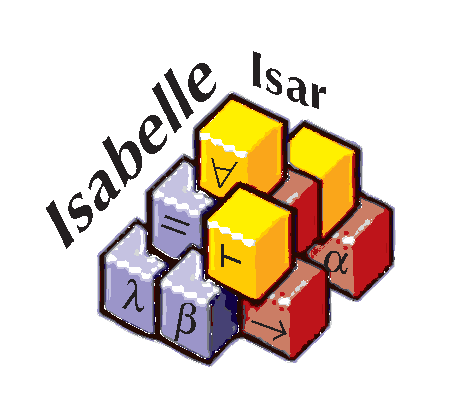
\includegraphics[scale=0.5]{isabelle_isar}
  \\[4ex] The Isabelle/Isar Implementation}
\author{\emph{Makarius Wenzel}  \\[3ex]
  With Contributions by
  Stefan Berghofer, \\
  Florian Haftmann
  and Larry Paulson
}

\makeindex


\begin{document}

\maketitle

\begin{abstract}
  We describe the key concepts underlying the Isabelle/Isar
  implementation, including ML references for the most important
  functions.  The aim is to give some insight into the overall system
  architecture, and provide clues on implementing applications within
  this framework.
\end{abstract}

\vspace*{2.5cm}
\begin{quote}

  {\small\em Isabelle was not designed; it evolved.  Not everyone
    likes this idea.  Specification experts rightly abhor
    trial-and-error programming.  They suggest that no one should
    write a program without first writing a complete formal
    specification. But university departments are not software houses.
    Programs like Isabelle are not products: when they have served
    their purpose, they are discarded.}

  Lawrence C. Paulson, ``Isabelle: The Next 700 Theorem Provers''

  \vspace*{1cm}

  {\small\em As I did 20 years ago, I still fervently believe that the
    only way to make software secure, reliable, and fast is to make it
    small.  Fight features.}

  Andrew S. Tanenbaum

  \vspace*{1cm}

  {\small\em One thing that UNIX does not need is more features. It is
    successful in part because it has a small number of good ideas
    that work well together. Merely adding features does not make it
    easier for users to do things --- it just makes the manual
    thicker. The right solution in the right place is always more
    effective than haphazard hacking.}

  Rob Pike and Brian W. Kernighan

  \vspace*{1cm}

  {\small\em If you look at software today, through the lens of the
    history of engineering, it's certainly engineering of a sort--but
    it's the kind of engineering that people without the concept of
    the arch did. Most software today is very much like an Egyptian
    pyramid with millions of bricks piled on top of each other, with
    no structural integrity, but just done by brute force and
    thousands of slaves.}

  Alan Kay

\end{quote}

\thispagestyle{empty}\clearpage

\pagenumbering{roman}
\tableofcontents
\listoffigures
\clearfirst

\setcounter{chapter}{-1}

%
\begin{isabellebody}%
\def\isabellecontext{ML}%
%
\isadelimtheory
\isanewline
\isanewline
%
\endisadelimtheory
%
\isatagtheory
\isacommand{theory}\isamarkupfalse%
\ {\isachardoublequoteopen}ML{\isachardoublequoteclose}\ \isakeyword{imports}\ base\ \isakeyword{begin}%
\endisatagtheory
{\isafoldtheory}%
%
\isadelimtheory
%
\endisadelimtheory
%
\isamarkupchapter{Aesthetics of ML programming%
}
\isamarkuptrue%
%
\begin{isamarkuptext}%
FIXME%
\end{isamarkuptext}%
\isamarkuptrue%
%
\begin{isamarkuptext}%
This style guide is loosely based on
  \url{http://caml.inria.fr/resources/doc/guides/guidelines.en.html}.
%  FIMXE \url{http://www.cs.cornell.edu/Courses/cs312/2003sp/handouts/style.htm}

  Like any style guide, it should not be interpreted dogmatically.
  Instead, it forms a collection of recommendations which,
  if obeyed, result in code that is not considered to be
  obfuscated.  In certain cases, derivations are encouraged,
  as far as you know what you are doing.

  \begin{description}

    \item[fundamental law of programming]
      Whenever writing code, keep in mind: A program is
      written once, modified ten times, and read
      100 times.  So simplify its writing,
      always keep future modifications in mind,
      and never jeopardize readability.  Every second you hesitate
      to spend on making your code more clear you will
      have to spend ten times understanding what you have
      written later on.

    \item[white space matters]
      Treat white space in your code as if it determines
      the meaning of code.

      \begin{itemize}

        \item The space bar is the easiest key to find on the keyboard,
          press it as often as necessary. {\ttfamily 2 + 2} is better
          than {\ttfamily 2+2}, likewise {\ttfamily f (x, y)}
          better than {\ttfamily f(x,y)}.

        \item Restrict your lines to \emph{at most} 80 characters.
          This will allow you to keep the beginning of a line
          in view while watching its end.

        \item Ban tabs; they are a context-sensitive formatting
          feature and likely to confuse anyone not using your
          favourite editor.

        \item Get rid of trailing whitespace.  Instead, do not
          surpess a trailing newline at the end of your files.

        \item Choose a generally accepted style of indentation,
          then use it systematically throughout the whole
          application.  An indentation of two spaces is appropriate.
          Avoid dangling indentation.

      \end{itemize}

    \item[cut-and-paste succeeds over copy-and-paste]
      \emph{Never} copy-and-paste code when programming.  If you
        need the same piece of code twice, introduce a
        reasonable auxiliary function (if there is no
        such function, very likely you got something wrong).
        Any copy-and-paste will turn out to be painful 
        when something has to be changed or fixed later on.

    \item[comments]
      are a device which requires careful thinking before using
      it.  The best comment for your code should be the code itself.
      Prefer efforts to write clear, understandable code
      over efforts to explain nasty code.

    \item[functional programming is based on functions]
      Avoid ``constructivisms'', e.g. pass a table lookup function,
      rather than an actual table with lookup in body.  Accustom
      your way of codeing to the level of expressiveness
      a functional programming language is giving onto you.

    \item[tuples]
      are often in the way.  When there is no striking argument
      to tuple function arguments, just write your function curried.

    \item[telling names]
      Any name should tell its purpose as exactly as possible,
      while keeping its length to the absolutely neccessary minimum.
      Always give the same name to function arguments which
      have the same meaning. Separate words by underscores
      (``\verb|int_of_string|'', not ``\verb|intOfString|'')

  \end{description}%
\end{isamarkuptext}%
\isamarkuptrue%
%
\isamarkupchapter{Basic library functions%
}
\isamarkuptrue%
%
\begin{isamarkuptext}%
Beyond the proposal of the SML/NJ basis library, Isabelle comes
  with its own library, from which selected parts are given here.
  See further files \emph{Pure/library.ML} and \emph{Pure/General/*.ML}.%
\end{isamarkuptext}%
\isamarkuptrue%
%
\isamarkupsection{Linear transformations%
}
\isamarkuptrue%
%
\isadelimmlref
%
\endisadelimmlref
%
\isatagmlref
%
\begin{isamarkuptext}%
\begin{mldecls}
  \indexml{(op |$>$)}\verb|(op |\verb,|,\verb|>): 'a * ('a -> 'b) -> 'b| \\
  \indexml{fold}\verb|fold: ('a -> 'b -> 'b) -> 'a list -> 'b -> 'b| \\
  \indexml{fold-rev}\verb|fold_rev: ('a -> 'b -> 'b) -> 'a list -> 'b -> 'b| \\
  \end{mldecls}%
\end{isamarkuptext}%
\isamarkuptrue%
%
\endisatagmlref
{\isafoldmlref}%
%
\isadelimmlref
%
\endisadelimmlref
%
\isadelimML
%
\endisadelimML
%
\isatagML
%
\endisatagML
{\isafoldML}%
%
\isadelimML
%
\endisadelimML
%
\begin{isamarkuptext}%
Many problems in functional programming can be thought of
  as linear transformations, i.e.~a caluclation starts with a
  particular value \isa{x\ {\isasymColon}\ foo} which is then transformed
  by application of a function \isa{f\ {\isasymColon}\ foo\ {\isasymRightarrow}\ foo},
  continued by an application of a function \isa{g\ {\isasymColon}\ foo\ {\isasymRightarrow}\ bar},
  and so on.  As a canoncial example, take primitive functions enriching
  theories by constants and definitions:
  \verb|Sign.add_consts_i: (string * typ * mixfix) list -> theory|\isasep\isanewline%
\verb|-> theory|
  and \verb|Theory.add_defs_i: bool -> bool|\isasep\isanewline%
\verb|-> (bstring * term) list -> theory -> theory|.
  Written with naive application, an addition of a constant with
  a corresponding definition would look like:
  \verb|Theory.add_defs_i false false [dummy_def]|\isasep\isanewline%
\verb|  (Sign.add_consts_i [dummy_const] thy)|.
  With increasing numbers of applications, this code gets quite unreadable.
  Using composition, at least the nesting of brackets may be reduced:
  \verb|(Theory.add_defs_i false false [dummy_def] o Sign.add_consts_i|\isasep\isanewline%
\verb|  [dummy_const]) thy|.
  What remains unsatisfactory is that things are written down in the opposite order
  as they actually ``happen''.%
\end{isamarkuptext}%
\isamarkuptrue%
%
\isadelimML
%
\endisadelimML
%
\isatagML
%
\endisatagML
{\isafoldML}%
%
\isadelimML
%
\endisadelimML
%
\begin{isamarkuptext}%
At this stage, Isabelle offers some combinators which allow for more convenient
  notation, most notably reverse application:
  \isasep\isanewline%
\verb|thy|\isasep\isanewline%
\verb||\verb,|,\verb|> Sign.add_consts_i [dummy_const]|\isasep\isanewline%
\verb||\verb,|,\verb|> Theory.add_defs_i false false [dummy_def]|%
\end{isamarkuptext}%
\isamarkuptrue%
%
\begin{isamarkuptext}%
\noindent When iterating over a list of parameters \isa{{\isacharbrackleft}x\isactrlisub {\isadigit{1}}{\isacharcomma}\ x\isactrlisub {\isadigit{2}}{\isacharcomma}\ {\isasymdots}\ x\isactrlisub n{\isacharbrackright}\ {\isasymColon}\ {\isacharprime}a\ list},
  the \verb|fold| combinator lifts a single function \isa{f\ {\isasymColon}\ {\isacharprime}a\ {\isacharminus}{\isachargreater}\ {\isacharprime}b\ {\isacharminus}{\isachargreater}\ {\isacharprime}b}:
  \isa{y\ {\isacharbar}{\isachargreater}\ fold\ f\ {\isacharbrackleft}x\isactrlisub {\isadigit{1}}{\isacharcomma}\ x\isactrlisub {\isadigit{2}}{\isacharcomma}\ {\isasymdots}\ x\isactrlisub n{\isacharbrackright}\ {\isasymequiv}\ y\ {\isacharbar}{\isachargreater}\ f\ x\isactrlisub {\isadigit{1}}\ {\isacharbar}{\isachargreater}\ f\ x\isactrlisub {\isadigit{2}}\ {\isacharbar}{\isachargreater}\ {\isasymdots}\ {\isacharbar}{\isachargreater}\ f\ x\isactrlisub n}%
\end{isamarkuptext}%
\isamarkuptrue%
%
\isadelimmlref
%
\endisadelimmlref
%
\isatagmlref
%
\begin{isamarkuptext}%
\begin{mldecls}
  \indexml{(op |-$>$)}\verb|(op |\verb,|,\verb|->): ('c * 'a) * ('c -> 'a -> 'b) -> 'b| \\
  \indexml{(op |$>$$>$)}\verb|(op |\verb,|,\verb|>>): ('a * 'c) * ('a -> 'b) -> 'b * 'c| \\
  \indexml{(op ||$>$)}\verb|(op |\verb,|,\verb||\verb,|,\verb|>): ('c * 'a) * ('a -> 'b) -> 'c * 'b| \\
  \indexml{(op ||$>$$>$)}\verb|(op |\verb,|,\verb||\verb,|,\verb|>>): ('c * 'a) * ('a -> 'd * 'b) -> ('c * 'd) * 'b| \\
  \indexml{fold-map}\verb|fold_map: ('a -> 'b -> 'c * 'b) -> 'a list -> 'b -> 'c list * 'b| \\
  \end{mldecls}%
\end{isamarkuptext}%
\isamarkuptrue%
%
\endisatagmlref
{\isafoldmlref}%
%
\isadelimmlref
%
\endisadelimmlref
%
\begin{isamarkuptext}%
\noindent FIXME transformations involving side results%
\end{isamarkuptext}%
\isamarkuptrue%
%
\isadelimmlref
%
\endisadelimmlref
%
\isatagmlref
%
\begin{isamarkuptext}%
\begin{mldecls}
  \indexml{(op \#$>$)}\verb|(op #>): ('a -> 'b) * ('b -> 'c) -> 'a -> 'c| \\
  \indexml{(op \#-$>$)}\verb|(op #->): ('a -> 'c * 'b) * ('c -> 'b -> 'd) -> 'a -> 'd| \\
  \indexml{(op \#$>$$>$)}\verb|(op #>>): ('a -> 'c * 'b) * ('c -> 'd) -> 'a -> 'd * 'b| \\
  \indexml{(op \#\#$>$)}\verb|(op ##>): ('a -> 'c * 'b) * ('b -> 'd) -> 'a -> 'c * 'd| \\
  \indexml{(op \#\#$>$$>$)}\verb|(op ##>>): ('a -> 'c * 'b) * ('b -> 'e * 'd) -> 'a -> ('c * 'e) * 'd| \\
  \end{mldecls}%
\end{isamarkuptext}%
\isamarkuptrue%
%
\endisatagmlref
{\isafoldmlref}%
%
\isadelimmlref
%
\endisadelimmlref
%
\begin{isamarkuptext}%
\noindent All those linear combinators also exist in higher-order
  variants which do not expect a value on the left hand side
  but a function.%
\end{isamarkuptext}%
\isamarkuptrue%
%
\isadelimmlref
%
\endisadelimmlref
%
\isatagmlref
%
\begin{isamarkuptext}%
\begin{mldecls}
  \indexml{(op `)}\verb|(op `): ('b -> 'a) -> 'b -> 'a * 'b| \\
  \indexml{tap}\verb|tap: ('b -> 'a) -> 'b -> 'b| \\
  \end{mldecls}%
\end{isamarkuptext}%
\isamarkuptrue%
%
\endisatagmlref
{\isafoldmlref}%
%
\isadelimmlref
%
\endisadelimmlref
%
\begin{isamarkuptext}%
\noindent FIXME%
\end{isamarkuptext}%
\isamarkuptrue%
%
\isamarkupsection{Options and partiality%
}
\isamarkuptrue%
%
\isadelimmlref
%
\endisadelimmlref
%
\isatagmlref
%
\begin{isamarkuptext}%
\begin{mldecls}
  \indexml{is-some}\verb|is_some: 'a option -> bool| \\
  \indexml{is-none}\verb|is_none: 'a option -> bool| \\
  \indexml{the}\verb|the: 'a option -> 'a| \\
  \indexml{these}\verb|these: 'a list option -> 'a list| \\
  \indexml{the-list}\verb|the_list: 'a option -> 'a list| \\
  \indexml{the-default}\verb|the_default: 'a -> 'a option -> 'a| \\
  \indexml{try}\verb|try: ('a -> 'b) -> 'a -> 'b option| \\
  \indexml{can}\verb|can: ('a -> 'b) -> 'a -> bool| \\
  \end{mldecls}%
\end{isamarkuptext}%
\isamarkuptrue%
%
\endisatagmlref
{\isafoldmlref}%
%
\isadelimmlref
%
\endisadelimmlref
%
\begin{isamarkuptext}%
Standard selector functions on \isa{option}s are provided.
  The \verb|try| and \verb|can| functions provide a convenient
  interface for handling exceptions -- both take as arguments
  a function \isa{f} together with a parameter \isa{x}
  and catch any exception during the evaluation of the application
  of \isa{f} to \isa{x}, either return a lifted result
  (\verb|NONE| on failure) or a boolean value (\verb|false| on failure).%
\end{isamarkuptext}%
\isamarkuptrue%
%
\isamarkupsection{Common data structures%
}
\isamarkuptrue%
%
\isamarkupsubsection{Lists (as set-like data structures)%
}
\isamarkuptrue%
%
\begin{isamarkuptext}%
\begin{mldecls}
  \indexml{member}\verb|member: ('b * 'a -> bool) -> 'a list -> 'b -> bool| \\
  \indexml{insert}\verb|insert: ('a * 'a -> bool) -> 'a -> 'a list -> 'a list| \\
  \indexml{remove}\verb|remove: ('b * 'a -> bool) -> 'b -> 'a list -> 'a list| \\
  \indexml{merge}\verb|merge: ('a * 'a -> bool) -> 'a list * 'a list -> 'a list| \\
  \end{mldecls}%
\end{isamarkuptext}%
\isamarkuptrue%
%
\begin{isamarkuptext}%
Lists are often used as set-like data structures -- set-like in
  then sense that they support notion of \verb|member|-ship,
  \verb|insert|-ing and \verb|remove|-ing, but are order-sensitive.
  This is convenient when implementing a history-like mechanism:
  \verb|insert| adds an element \emph{to the front} of a list,
  if not yet present; \verb|remove| removes \emph{all} occurences
  of a particular element.  Correspondingly \verb|merge| implements a 
  a merge on two lists suitable for merges of context data
  (\secref{sec:context-theory}).

  Functions are parametrized by an explicit equality function
  to accomplish overloaded equality;  in most cases of monomorphic
  equality, writing \verb|(op =)| should suffice.%
\end{isamarkuptext}%
\isamarkuptrue%
%
\isamarkupsubsection{Association lists%
}
\isamarkuptrue%
%
\begin{isamarkuptext}%
\begin{mldecls}
  \indexmlexception{AList.DUP}\verb|exception AList.DUP| \\
  \indexml{AList.lookup}\verb|AList.lookup: ('a * 'b -> bool) -> ('b * 'c) list -> 'a -> 'c option| \\
  \indexml{AList.defined}\verb|AList.defined: ('a * 'b -> bool) -> ('b * 'c) list -> 'a -> bool| \\
  \indexml{AList.update}\verb|AList.update: ('a * 'a -> bool) -> ('a * 'b) -> ('a * 'b) list -> ('a * 'b) list| \\
  \indexml{AList.default}\verb|AList.default: ('a * 'a -> bool) -> ('a * 'b) -> ('a * 'b) list -> ('a * 'b) list| \\
  \indexml{AList.delete}\verb|AList.delete: ('a * 'b -> bool) -> 'a -> ('b * 'c) list -> ('b * 'c) list| \\
  \indexml{AList.map-entry}\verb|AList.map_entry: ('a * 'b -> bool) -> 'a|\isasep\isanewline%
\verb|    -> ('c -> 'c) -> ('b * 'c) list -> ('b * 'c) list| \\
  \indexml{AList.map-default}\verb|AList.map_default: ('a * 'a -> bool) -> 'a * 'b -> ('b -> 'b)|\isasep\isanewline%
\verb|    -> ('a * 'b) list -> ('a * 'b) list| \\
  \indexml{AList.join}\verb|AList.join: ('a * 'a -> bool) -> ('a -> 'b * 'b -> 'b) (*exception DUP*)|\isasep\isanewline%
\verb|    -> ('a * 'b) list * ('a * 'b) list -> ('a * 'b) list (*exception AList.DUP*)| \\
  \indexml{AList.merge}\verb|AList.merge: ('a * 'a -> bool) -> ('b * 'b -> bool)|\isasep\isanewline%
\verb|    -> ('a * 'b) list * ('a * 'b) list -> ('a * 'b) list (*exception AList.DUP*)|
  \end{mldecls}%
\end{isamarkuptext}%
\isamarkuptrue%
%
\begin{isamarkuptext}%
Association lists can be seens as an extension of set-like lists:
  on the one hand, they may be used to implement finite mappings,
  on the other hand, they remain order-sensitive and allow for
  multiple key-value-pair with the same key: \verb|AList.lookup|
  returns the \emph{first} value corresponding to a particular
  key, if present.  \verb|AList.update| updates
  the \emph{first} occurence of a particular key; if no such
  key exists yet, the key-value-pair is added \emph{to the front}.
  \verb|AList.delete| only deletes the \emph{first} occurence of a key.
  \verb|AList.merge| provides an operation suitable for merges of context data
  (\secref{sec:context-theory}), where an equality parameter on
  values determines whether a merge should be considered a conflict.
  A slightly generalized operation if implementend by the \verb|AList.join|
  function which allows for explicit conflict resolution.%
\end{isamarkuptext}%
\isamarkuptrue%
%
\isamarkupsubsection{Tables%
}
\isamarkuptrue%
%
\begin{isamarkuptext}%
\begin{mldecls}
  \indexmltype{Symtab.key}\verb|type Symtab.key| \\
  \indexmltype{'a Symtab.table}\verb|type 'a Symtab.table| \\
  \indexmlexception{Symtab.DUP}\verb|exception Symtab.DUP of Symtab.key| \\
  \indexmlexception{Symtab.DUPS}\verb|exception Symtab.DUPS of Symtab.key list| \\
  \indexmlexception{Symtab.SAME}\verb|exception Symtab.SAME| \\
  \indexmlexception{Symtab.UNDEF}\verb|exception Symtab.UNDEF of Symtab.key| \\
  \indexml{Symtab.empty}\verb|Symtab.empty: 'a Symtab.table| \\
  \indexml{Symtab.dest}\verb|Symtab.dest: 'a Symtab.table -> (Symtab.key * 'a) list| \\
  \indexml{Symtab.keys}\verb|Symtab.keys: 'a Symtab.table -> Symtab.key list| \\
  \indexml{Symtab.lookup}\verb|Symtab.lookup: 'a Symtab.table -> Symtab.key -> 'a option| \\
  \indexml{Symtab.defined}\verb|Symtab.defined: 'a Symtab.table -> Symtab.key -> bool| \\
  \indexml{Symtab.update}\verb|Symtab.update: (Symtab.key * 'a) -> 'a Symtab.table -> 'a Symtab.table| \\
  \indexml{Symtab.default}\verb|Symtab.default: Symtab.key * 'a -> 'a Symtab.table -> 'a Symtab.table| \\
  \indexml{Symtab.delete}\verb|Symtab.delete: Symtab.key|\isasep\isanewline%
\verb|    -> 'a Symtab.table -> 'a Symtab.table (*exception Symtab.UNDEF*)| \\
  \indexml{Symtab.map-entry}\verb|Symtab.map_entry: Symtab.key -> ('a -> 'a)|\isasep\isanewline%
\verb|    -> 'a Symtab.table -> 'a Symtab.table| \\
  \indexml{Symtab.map-default}\verb|Symtab.map_default: (Symtab.key * 'a) -> ('a -> 'a)|\isasep\isanewline%
\verb|    -> 'a Symtab.table -> 'a Symtab.table| \\
  \indexml{Symtab.join}\verb|Symtab.join: (Symtab.key -> 'a * 'a -> 'a) (*exception Symtab.DUP/Symtab.SAME*)|\isasep\isanewline%
\verb|    -> 'a Symtab.table * 'a Symtab.table|\isasep\isanewline%
\verb|    -> 'a Symtab.table (*exception Symtab.DUPS*)| \\
  \indexml{Symtab.merge}\verb|Symtab.merge: ('a * 'a -> bool)|\isasep\isanewline%
\verb|    -> 'a Symtab.table * 'a Symtab.table|\isasep\isanewline%
\verb|    -> 'a Symtab.table (*exception Symtab.DUPS*)|
  \end{mldecls}%
\end{isamarkuptext}%
\isamarkuptrue%
%
\begin{isamarkuptext}%
Tables are an efficient representation of finite mappings without
  any notion of order;  due to their efficiency they should be used
  whenever such pure finite mappings are neccessary.

  The key type of tables must be given explicitly by instantiating
  the \verb|TableFun| functor which takes the key type
  together with its \verb|order|; for convience, we restrict
  here to the \verb|Symtab| instance with \verb|string|
  as key type.

  Most table functions correspond to those of association lists.%
\end{isamarkuptext}%
\isamarkuptrue%
%
\isamarkupchapter{Cookbook%
}
\isamarkuptrue%
%
\isamarkupsection{A method that depends on declarations in the context%
}
\isamarkuptrue%
%
\begin{isamarkuptext}%
FIXME%
\end{isamarkuptext}%
\isamarkuptrue%
%
\isadelimtheory
%
\endisadelimtheory
%
\isatagtheory
\isacommand{end}\isamarkupfalse%
%
\endisatagtheory
{\isafoldtheory}%
%
\isadelimtheory
%
\endisadelimtheory
\isanewline
\end{isabellebody}%
%%% Local Variables:
%%% mode: latex
%%% TeX-master: "root"
%%% End:

%
\begin{isabellebody}%
\def\isabellecontext{Prelim}%
%
\isadelimtheory
%
\endisadelimtheory
%
\isatagtheory
\isacommand{theory}\isamarkupfalse%
\ Prelim\isanewline
\isakeyword{imports}\ Base\isanewline
\isakeyword{begin}%
\endisatagtheory
{\isafoldtheory}%
%
\isadelimtheory
%
\endisadelimtheory
%
\isamarkupchapter{Preliminaries%
}
\isamarkuptrue%
%
\isamarkupsection{Contexts \label{sec:context}%
}
\isamarkuptrue%
%
\begin{isamarkuptext}%
A logical context represents the background that is required for
  formulating statements and composing proofs.  It acts as a medium to
  produce formal content, depending on earlier material (declarations,
  results etc.).

  For example, derivations within the Isabelle/Pure logic can be
  described as a judgment \isa{{\isaliteral{5C3C47616D6D613E}{\isasymGamma}}\ {\isaliteral{5C3C7475726E7374696C653E}{\isasymturnstile}}\isaliteral{5C3C5E7375623E}{}\isactrlsub {\isaliteral{5C3C54686574613E}{\isasymTheta}}\ {\isaliteral{5C3C7068693E}{\isasymphi}}}, which means that a
  proposition \isa{{\isaliteral{5C3C7068693E}{\isasymphi}}} is derivable from hypotheses \isa{{\isaliteral{5C3C47616D6D613E}{\isasymGamma}}}
  within the theory \isa{{\isaliteral{5C3C54686574613E}{\isasymTheta}}}.  There are logical reasons for
  keeping \isa{{\isaliteral{5C3C54686574613E}{\isasymTheta}}} and \isa{{\isaliteral{5C3C47616D6D613E}{\isasymGamma}}} separate: theories can be
  liberal about supporting type constructors and schematic
  polymorphism of constants and axioms, while the inner calculus of
  \isa{{\isaliteral{5C3C47616D6D613E}{\isasymGamma}}\ {\isaliteral{5C3C7475726E7374696C653E}{\isasymturnstile}}\ {\isaliteral{5C3C7068693E}{\isasymphi}}} is strictly limited to Simple Type Theory (with
  fixed type variables in the assumptions).

  \medskip Contexts and derivations are linked by the following key
  principles:

  \begin{itemize}

  \item Transfer: monotonicity of derivations admits results to be
  transferred into a \emph{larger} context, i.e.\ \isa{{\isaliteral{5C3C47616D6D613E}{\isasymGamma}}\ {\isaliteral{5C3C7475726E7374696C653E}{\isasymturnstile}}\isaliteral{5C3C5E7375623E}{}\isactrlsub {\isaliteral{5C3C54686574613E}{\isasymTheta}}\ {\isaliteral{5C3C7068693E}{\isasymphi}}} implies \isa{{\isaliteral{5C3C47616D6D613E}{\isasymGamma}}{\isaliteral{27}{\isacharprime}}\ {\isaliteral{5C3C7475726E7374696C653E}{\isasymturnstile}}\isaliteral{5C3C5E7375623E}{}\isactrlsub {\isaliteral{5C3C54686574613E}{\isasymTheta}}\isaliteral{5C3C5E7375623E}{}\isactrlsub {\isaliteral{27}{\isacharprime}}\ {\isaliteral{5C3C7068693E}{\isasymphi}}} for contexts \isa{{\isaliteral{5C3C54686574613E}{\isasymTheta}}{\isaliteral{27}{\isacharprime}}\ {\isaliteral{5C3C73757073657465713E}{\isasymsupseteq}}\ {\isaliteral{5C3C54686574613E}{\isasymTheta}}} and \isa{{\isaliteral{5C3C47616D6D613E}{\isasymGamma}}{\isaliteral{27}{\isacharprime}}\ {\isaliteral{5C3C73757073657465713E}{\isasymsupseteq}}\ {\isaliteral{5C3C47616D6D613E}{\isasymGamma}}}.

  \item Export: discharge of hypotheses admits results to be exported
  into a \emph{smaller} context, i.e.\ \isa{{\isaliteral{5C3C47616D6D613E}{\isasymGamma}}{\isaliteral{27}{\isacharprime}}\ {\isaliteral{5C3C7475726E7374696C653E}{\isasymturnstile}}\isaliteral{5C3C5E7375623E}{}\isactrlsub {\isaliteral{5C3C54686574613E}{\isasymTheta}}\ {\isaliteral{5C3C7068693E}{\isasymphi}}}
  implies \isa{{\isaliteral{5C3C47616D6D613E}{\isasymGamma}}\ {\isaliteral{5C3C7475726E7374696C653E}{\isasymturnstile}}\isaliteral{5C3C5E7375623E}{}\isactrlsub {\isaliteral{5C3C54686574613E}{\isasymTheta}}\ {\isaliteral{5C3C44656C74613E}{\isasymDelta}}\ {\isaliteral{5C3C4C6F6E6772696768746172726F773E}{\isasymLongrightarrow}}\ {\isaliteral{5C3C7068693E}{\isasymphi}}} where \isa{{\isaliteral{5C3C47616D6D613E}{\isasymGamma}}{\isaliteral{27}{\isacharprime}}\ {\isaliteral{5C3C73757073657465713E}{\isasymsupseteq}}\ {\isaliteral{5C3C47616D6D613E}{\isasymGamma}}} and
  \isa{{\isaliteral{5C3C44656C74613E}{\isasymDelta}}\ {\isaliteral{3D}{\isacharequal}}\ {\isaliteral{5C3C47616D6D613E}{\isasymGamma}}{\isaliteral{27}{\isacharprime}}\ {\isaliteral{2D}{\isacharminus}}\ {\isaliteral{5C3C47616D6D613E}{\isasymGamma}}}.  Note that \isa{{\isaliteral{5C3C54686574613E}{\isasymTheta}}} remains unchanged here,
  only the \isa{{\isaliteral{5C3C47616D6D613E}{\isasymGamma}}} part is affected.

  \end{itemize}

  \medskip By modeling the main characteristics of the primitive
  \isa{{\isaliteral{5C3C54686574613E}{\isasymTheta}}} and \isa{{\isaliteral{5C3C47616D6D613E}{\isasymGamma}}} above, and abstracting over any
  particular logical content, we arrive at the fundamental notions of
  \emph{theory context} and \emph{proof context} in Isabelle/Isar.
  These implement a certain policy to manage arbitrary \emph{context
  data}.  There is a strongly-typed mechanism to declare new kinds of
  data at compile time.

  The internal bootstrap process of Isabelle/Pure eventually reaches a
  stage where certain data slots provide the logical content of \isa{{\isaliteral{5C3C54686574613E}{\isasymTheta}}} and \isa{{\isaliteral{5C3C47616D6D613E}{\isasymGamma}}} sketched above, but this does not stop there!
  Various additional data slots support all kinds of mechanisms that
  are not necessarily part of the core logic.

  For example, there would be data for canonical introduction and
  elimination rules for arbitrary operators (depending on the
  object-logic and application), which enables users to perform
  standard proof steps implicitly (cf.\ the \isa{rule} method
  \cite{isabelle-isar-ref}).

  \medskip Thus Isabelle/Isar is able to bring forth more and more
  concepts successively.  In particular, an object-logic like
  Isabelle/HOL continues the Isabelle/Pure setup by adding specific
  components for automated reasoning (classical reasoner, tableau
  prover, structured induction etc.) and derived specification
  mechanisms (inductive predicates, recursive functions etc.).  All of
  this is ultimately based on the generic data management by theory
  and proof contexts introduced here.%
\end{isamarkuptext}%
\isamarkuptrue%
%
\isamarkupsubsection{Theory context \label{sec:context-theory}%
}
\isamarkuptrue%
%
\begin{isamarkuptext}%
A \emph{theory} is a data container with explicit name and
  unique identifier.  Theories are related by a (nominal) sub-theory
  relation, which corresponds to the dependency graph of the original
  construction; each theory is derived from a certain sub-graph of
  ancestor theories.  To this end, the system maintains a set of
  symbolic ``identification stamps'' within each theory.

  In order to avoid the full-scale overhead of explicit sub-theory
  identification of arbitrary intermediate stages, a theory is
  switched into \isa{draft} mode under certain circumstances.  A
  draft theory acts like a linear type, where updates invalidate
  earlier versions.  An invalidated draft is called \emph{stale}.

  The \isa{checkpoint} operation produces a safe stepping stone
  that will survive the next update without becoming stale: both the
  old and the new theory remain valid and are related by the
  sub-theory relation.  Checkpointing essentially recovers purely
  functional theory values, at the expense of some extra internal
  bookkeeping.

  The \isa{copy} operation produces an auxiliary version that has
  the same data content, but is unrelated to the original: updates of
  the copy do not affect the original, neither does the sub-theory
  relation hold.

  The \isa{merge} operation produces the least upper bound of two
  theories, which actually degenerates into absorption of one theory
  into the other (according to the nominal sub-theory relation).

  The \isa{begin} operation starts a new theory by importing
  several parent theories and entering a special mode of nameless
  incremental updates, until the final \isa{end} operation is
  performed.

  \medskip The example in \figref{fig:ex-theory} below shows a theory
  graph derived from \isa{Pure}, with theory \isa{Length}
  importing \isa{Nat} and \isa{List}.  The body of \isa{Length} consists of a sequence of updates, working mostly on
  drafts internally, while transaction boundaries of Isar top-level
  commands (\secref{sec:isar-toplevel}) are guaranteed to be safe
  checkpoints.

  \begin{figure}[htb]
  \begin{center}
  \begin{tabular}{rcccl}
        &            & \isa{Pure} \\
        &            & \isa{{\isaliteral{5C3C646F776E3E}{\isasymdown}}} \\
        &            & \isa{FOL} \\
        & $\swarrow$ &              & $\searrow$ & \\
  \isa{Nat} &    &              &            & \isa{List} \\
        & $\searrow$ &              & $\swarrow$ \\
        &            & \isa{Length} \\
        &            & \multicolumn{3}{l}{~~\hyperlink{keyword.imports}{\mbox{\isa{\isakeyword{imports}}}}} \\
        &            & \multicolumn{3}{l}{~~\hyperlink{keyword.begin}{\mbox{\isa{\isakeyword{begin}}}}} \\
        &            & $\vdots$~~ \\
        &            & \isa{{\isaliteral{5C3C62756C6C65743E}{\isasymbullet}}}~~ \\
        &            & $\vdots$~~ \\
        &            & \isa{{\isaliteral{5C3C62756C6C65743E}{\isasymbullet}}}~~ \\
        &            & $\vdots$~~ \\
        &            & \multicolumn{3}{l}{~~\hyperlink{command.end}{\mbox{\isa{\isacommand{end}}}}} \\
  \end{tabular}
  \caption{A theory definition depending on ancestors}\label{fig:ex-theory}
  \end{center}
  \end{figure}

  \medskip There is a separate notion of \emph{theory reference} for
  maintaining a live link to an evolving theory context: updates on
  drafts are propagated automatically.  Dynamic updating stops when
  the next \isa{checkpoint} is reached.

  Derived entities may store a theory reference in order to indicate
  the formal context from which they are derived.  This implicitly
  assumes monotonic reasoning, because the referenced context may
  become larger without further notice.%
\end{isamarkuptext}%
\isamarkuptrue%
%
\isadelimmlref
%
\endisadelimmlref
%
\isatagmlref
%
\begin{isamarkuptext}%
\begin{mldecls}
  \indexdef{}{ML type}{theory}\verb|type theory| \\
  \indexdef{}{ML}{Theory.eq\_thy}\verb|Theory.eq_thy: theory * theory -> bool| \\
  \indexdef{}{ML}{Theory.subthy}\verb|Theory.subthy: theory * theory -> bool| \\
  \indexdef{}{ML}{Theory.checkpoint}\verb|Theory.checkpoint: theory -> theory| \\
  \indexdef{}{ML}{Theory.copy}\verb|Theory.copy: theory -> theory| \\
  \indexdef{}{ML}{Theory.merge}\verb|Theory.merge: theory * theory -> theory| \\
  \indexdef{}{ML}{Theory.begin\_theory}\verb|Theory.begin_theory: string -> theory list -> theory| \\
  \indexdef{}{ML}{Theory.parents\_of}\verb|Theory.parents_of: theory -> theory list| \\
  \indexdef{}{ML}{Theory.ancestors\_of}\verb|Theory.ancestors_of: theory -> theory list| \\
  \end{mldecls}
  \begin{mldecls}
  \indexdef{}{ML type}{theory\_ref}\verb|type theory_ref| \\
  \indexdef{}{ML}{Theory.deref}\verb|Theory.deref: theory_ref -> theory| \\
  \indexdef{}{ML}{Theory.check\_thy}\verb|Theory.check_thy: theory -> theory_ref| \\
  \end{mldecls}

  \begin{description}

  \item Type \verb|theory| represents theory contexts.  This is
  essentially a linear type, with explicit runtime checking.
  Primitive theory operations destroy the original version, which then
  becomes ``stale''.  This can be prevented by explicit checkpointing,
  which the system does at least at the boundary of toplevel command
  transactions \secref{sec:isar-toplevel}.

  \item \verb|Theory.eq_thy|~\isa{{\isaliteral{28}{\isacharparenleft}}thy\isaliteral{5C3C5E7375623E}{}\isactrlsub {\isadigit{1}}{\isaliteral{2C}{\isacharcomma}}\ thy\isaliteral{5C3C5E7375623E}{}\isactrlsub {\isadigit{2}}{\isaliteral{29}{\isacharparenright}}} check strict
  identity of two theories.

  \item \verb|Theory.subthy|~\isa{{\isaliteral{28}{\isacharparenleft}}thy\isaliteral{5C3C5E7375623E}{}\isactrlsub {\isadigit{1}}{\isaliteral{2C}{\isacharcomma}}\ thy\isaliteral{5C3C5E7375623E}{}\isactrlsub {\isadigit{2}}{\isaliteral{29}{\isacharparenright}}} compares theories
  according to the intrinsic graph structure of the construction.
  This sub-theory relation is a nominal approximation of inclusion
  (\isa{{\isaliteral{5C3C73756273657465713E}{\isasymsubseteq}}}) of the corresponding content (according to the
  semantics of the ML modules that implement the data).

  \item \verb|Theory.checkpoint|~\isa{thy} produces a safe
  stepping stone in the linear development of \isa{thy}.  This
  changes the old theory, but the next update will result in two
  related, valid theories.

  \item \verb|Theory.copy|~\isa{thy} produces a variant of \isa{thy} with the same data.  The copy is not related to the original,
  but the original is unchanged.

  \item \verb|Theory.merge|~\isa{{\isaliteral{28}{\isacharparenleft}}thy\isaliteral{5C3C5E7375623E}{}\isactrlsub {\isadigit{1}}{\isaliteral{2C}{\isacharcomma}}\ thy\isaliteral{5C3C5E7375623E}{}\isactrlsub {\isadigit{2}}{\isaliteral{29}{\isacharparenright}}} absorbs one theory
  into the other, without changing \isa{thy\isaliteral{5C3C5E7375623E}{}\isactrlsub {\isadigit{1}}} or \isa{thy\isaliteral{5C3C5E7375623E}{}\isactrlsub {\isadigit{2}}}.
  This version of ad-hoc theory merge fails for unrelated theories!

  \item \verb|Theory.begin_theory|~\isa{name\ parents} constructs
  a new theory based on the given parents.  This ML function is
  normally not invoked directly.

  \item \verb|Theory.parents_of|~\isa{thy} returns the direct
  ancestors of \isa{thy}.

  \item \verb|Theory.ancestors_of|~\isa{thy} returns all
  ancestors of \isa{thy} (not including \isa{thy} itself).

  \item Type \verb|theory_ref| represents a sliding reference to
  an always valid theory; updates on the original are propagated
  automatically.

  \item \verb|Theory.deref|~\isa{thy{\isaliteral{5F}{\isacharunderscore}}ref} turns a \verb|theory_ref| into an \verb|theory| value.  As the referenced
  theory evolves monotonically over time, later invocations of \verb|Theory.deref| may refer to a larger context.

  \item \verb|Theory.check_thy|~\isa{thy} produces a \verb|theory_ref| from a valid \verb|theory| value.

  \end{description}%
\end{isamarkuptext}%
\isamarkuptrue%
%
\endisatagmlref
{\isafoldmlref}%
%
\isadelimmlref
%
\endisadelimmlref
%
\isadelimmlantiq
%
\endisadelimmlantiq
%
\isatagmlantiq
%
\begin{isamarkuptext}%
\begin{matharray}{rcl}
  \indexdef{}{ML antiquotation}{theory}\hypertarget{ML antiquotation.theory}{\hyperlink{ML antiquotation.theory}{\mbox{\isa{theory}}}} & : & \isa{ML{\isaliteral{5F}{\isacharunderscore}}antiquotation} \\
  \end{matharray}

  \begin{railoutput}
\rail@begin{2}{}
\rail@term{\hyperlink{ML antiquotation.theory}{\mbox{\isa{theory}}}}[]
\rail@bar
\rail@nextbar{1}
\rail@nont{\isa{nameref}}[]
\rail@endbar
\rail@end
\end{railoutput}


  \begin{description}

  \item \isa{{\isaliteral{40}{\isacharat}}{\isaliteral{7B}{\isacharbraceleft}}theory{\isaliteral{7D}{\isacharbraceright}}} refers to the background theory of the
  current context --- as abstract value.

  \item \isa{{\isaliteral{40}{\isacharat}}{\isaliteral{7B}{\isacharbraceleft}}theory\ A{\isaliteral{7D}{\isacharbraceright}}} refers to an explicitly named ancestor
  theory \isa{A} of the background theory of the current context
  --- as abstract value.

  \end{description}%
\end{isamarkuptext}%
\isamarkuptrue%
%
\endisatagmlantiq
{\isafoldmlantiq}%
%
\isadelimmlantiq
%
\endisadelimmlantiq
%
\isamarkupsubsection{Proof context \label{sec:context-proof}%
}
\isamarkuptrue%
%
\begin{isamarkuptext}%
A proof context is a container for pure data with a
  back-reference to the theory from which it is derived.  The \isa{init} operation creates a proof context from a given theory.
  Modifications to draft theories are propagated to the proof context
  as usual, but there is also an explicit \isa{transfer} operation
  to force resynchronization with more substantial updates to the
  underlying theory.

  Entities derived in a proof context need to record logical
  requirements explicitly, since there is no separate context
  identification or symbolic inclusion as for theories.  For example,
  hypotheses used in primitive derivations (cf.\ \secref{sec:thms})
  are recorded separately within the sequent \isa{{\isaliteral{5C3C47616D6D613E}{\isasymGamma}}\ {\isaliteral{5C3C7475726E7374696C653E}{\isasymturnstile}}\ {\isaliteral{5C3C7068693E}{\isasymphi}}}, just to
  make double sure.  Results could still leak into an alien proof
  context due to programming errors, but Isabelle/Isar includes some
  extra validity checks in critical positions, notably at the end of a
  sub-proof.

  Proof contexts may be manipulated arbitrarily, although the common
  discipline is to follow block structure as a mental model: a given
  context is extended consecutively, and results are exported back
  into the original context.  Note that an Isar proof state models
  block-structured reasoning explicitly, using a stack of proof
  contexts internally.  For various technical reasons, the background
  theory of an Isar proof state must not be changed while the proof is
  still under construction!%
\end{isamarkuptext}%
\isamarkuptrue%
%
\isadelimmlref
%
\endisadelimmlref
%
\isatagmlref
%
\begin{isamarkuptext}%
\begin{mldecls}
  \indexdef{}{ML type}{Proof.context}\verb|type Proof.context| \\
  \indexdef{}{ML}{Proof\_Context.init\_global}\verb|Proof_Context.init_global: theory -> Proof.context| \\
  \indexdef{}{ML}{Proof\_Context.theory\_of}\verb|Proof_Context.theory_of: Proof.context -> theory| \\
  \indexdef{}{ML}{Proof\_Context.transfer}\verb|Proof_Context.transfer: theory -> Proof.context -> Proof.context| \\
  \end{mldecls}

  \begin{description}

  \item Type \verb|Proof.context| represents proof contexts.
  Elements of this type are essentially pure values, with a sliding
  reference to the background theory.

  \item \verb|Proof_Context.init_global|~\isa{thy} produces a proof context
  derived from \isa{thy}, initializing all data.

  \item \verb|Proof_Context.theory_of|~\isa{ctxt} selects the
  background theory from \isa{ctxt}, dereferencing its internal
  \verb|theory_ref|.

  \item \verb|Proof_Context.transfer|~\isa{thy\ ctxt} promotes the
  background theory of \isa{ctxt} to the super theory \isa{thy}.

  \end{description}%
\end{isamarkuptext}%
\isamarkuptrue%
%
\endisatagmlref
{\isafoldmlref}%
%
\isadelimmlref
%
\endisadelimmlref
%
\isadelimmlantiq
%
\endisadelimmlantiq
%
\isatagmlantiq
%
\begin{isamarkuptext}%
\begin{matharray}{rcl}
  \indexdef{}{ML antiquotation}{context}\hypertarget{ML antiquotation.context}{\hyperlink{ML antiquotation.context}{\mbox{\isa{context}}}} & : & \isa{ML{\isaliteral{5F}{\isacharunderscore}}antiquotation} \\
  \end{matharray}

  \begin{description}

  \item \isa{{\isaliteral{40}{\isacharat}}{\isaliteral{7B}{\isacharbraceleft}}context{\isaliteral{7D}{\isacharbraceright}}} refers to \emph{the} context at
  compile-time --- as abstract value.  Independently of (local) theory
  or proof mode, this always produces a meaningful result.

  This is probably the most common antiquotation in interactive
  experimentation with ML inside Isar.

  \end{description}%
\end{isamarkuptext}%
\isamarkuptrue%
%
\endisatagmlantiq
{\isafoldmlantiq}%
%
\isadelimmlantiq
%
\endisadelimmlantiq
%
\isamarkupsubsection{Generic contexts \label{sec:generic-context}%
}
\isamarkuptrue%
%
\begin{isamarkuptext}%
A generic context is the disjoint sum of either a theory or proof
  context.  Occasionally, this enables uniform treatment of generic
  context data, typically extra-logical information.  Operations on
  generic contexts include the usual injections, partial selections,
  and combinators for lifting operations on either component of the
  disjoint sum.

  Moreover, there are total operations \isa{theory{\isaliteral{5F}{\isacharunderscore}}of} and \isa{proof{\isaliteral{5F}{\isacharunderscore}}of} to convert a generic context into either kind: a theory
  can always be selected from the sum, while a proof context might
  have to be constructed by an ad-hoc \isa{init} operation, which
  incurs a small runtime overhead.%
\end{isamarkuptext}%
\isamarkuptrue%
%
\isadelimmlref
%
\endisadelimmlref
%
\isatagmlref
%
\begin{isamarkuptext}%
\begin{mldecls}
  \indexdef{}{ML type}{Context.generic}\verb|type Context.generic| \\
  \indexdef{}{ML}{Context.theory\_of}\verb|Context.theory_of: Context.generic -> theory| \\
  \indexdef{}{ML}{Context.proof\_of}\verb|Context.proof_of: Context.generic -> Proof.context| \\
  \end{mldecls}

  \begin{description}

  \item Type \verb|Context.generic| is the direct sum of \verb|theory| and \verb|Proof.context|, with the datatype
  constructors \verb|Context.Theory| and \verb|Context.Proof|.

  \item \verb|Context.theory_of|~\isa{context} always produces a
  theory from the generic \isa{context}, using \verb|Proof_Context.theory_of| as required.

  \item \verb|Context.proof_of|~\isa{context} always produces a
  proof context from the generic \isa{context}, using \verb|Proof_Context.init_global| as required (note that this re-initializes the
  context data with each invocation).

  \end{description}%
\end{isamarkuptext}%
\isamarkuptrue%
%
\endisatagmlref
{\isafoldmlref}%
%
\isadelimmlref
%
\endisadelimmlref
%
\isamarkupsubsection{Context data \label{sec:context-data}%
}
\isamarkuptrue%
%
\begin{isamarkuptext}%
The main purpose of theory and proof contexts is to manage
  arbitrary (pure) data.  New data types can be declared incrementally
  at compile time.  There are separate declaration mechanisms for any
  of the three kinds of contexts: theory, proof, generic.

  \paragraph{Theory data} declarations need to implement the following
  SML signature:

  \medskip
  \begin{tabular}{ll}
  \isa{{\isaliteral{5C3C747970653E}{\isasymtype}}\ T} & representing type \\
  \isa{{\isaliteral{5C3C76616C3E}{\isasymval}}\ empty{\isaliteral{3A}{\isacharcolon}}\ T} & empty default value \\
  \isa{{\isaliteral{5C3C76616C3E}{\isasymval}}\ extend{\isaliteral{3A}{\isacharcolon}}\ T\ {\isaliteral{5C3C72696768746172726F773E}{\isasymrightarrow}}\ T} & re-initialize on import \\
  \isa{{\isaliteral{5C3C76616C3E}{\isasymval}}\ merge{\isaliteral{3A}{\isacharcolon}}\ T\ {\isaliteral{5C3C74696D65733E}{\isasymtimes}}\ T\ {\isaliteral{5C3C72696768746172726F773E}{\isasymrightarrow}}\ T} & join on import \\
  \end{tabular}
  \medskip

  The \isa{empty} value acts as initial default for \emph{any}
  theory that does not declare actual data content; \isa{extend}
  is acts like a unitary version of \isa{merge}.

  Implementing \isa{merge} can be tricky.  The general idea is
  that \isa{merge\ {\isaliteral{28}{\isacharparenleft}}data\isaliteral{5C3C5E7375623E}{}\isactrlsub {\isadigit{1}}{\isaliteral{2C}{\isacharcomma}}\ data\isaliteral{5C3C5E7375623E}{}\isactrlsub {\isadigit{2}}{\isaliteral{29}{\isacharparenright}}} inserts those parts of \isa{data\isaliteral{5C3C5E7375623E}{}\isactrlsub {\isadigit{2}}} into \isa{data\isaliteral{5C3C5E7375623E}{}\isactrlsub {\isadigit{1}}} that are not yet present, while
  keeping the general order of things.  The \verb|Library.merge|
  function on plain lists may serve as canonical template.

  Particularly note that shared parts of the data must not be
  duplicated by naive concatenation, or a theory graph that is like a
  chain of diamonds would cause an exponential blowup!

  \paragraph{Proof context data} declarations need to implement the
  following SML signature:

  \medskip
  \begin{tabular}{ll}
  \isa{{\isaliteral{5C3C747970653E}{\isasymtype}}\ T} & representing type \\
  \isa{{\isaliteral{5C3C76616C3E}{\isasymval}}\ init{\isaliteral{3A}{\isacharcolon}}\ theory\ {\isaliteral{5C3C72696768746172726F773E}{\isasymrightarrow}}\ T} & produce initial value \\
  \end{tabular}
  \medskip

  The \isa{init} operation is supposed to produce a pure value
  from the given background theory and should be somehow
  ``immediate''.  Whenever a proof context is initialized, which
  happens frequently, the the system invokes the \isa{init}
  operation of \emph{all} theory data slots ever declared.  This also
  means that one needs to be economic about the total number of proof
  data declarations in the system, i.e.\ each ML module should declare
  at most one, sometimes two data slots for its internal use.
  Repeated data declarations to simulate a record type should be
  avoided!

  \paragraph{Generic data} provides a hybrid interface for both theory
  and proof data.  The \isa{init} operation for proof contexts is
  predefined to select the current data value from the background
  theory.

  \bigskip Any of the above data declarations over type \isa{T}
  result in an ML structure with the following signature:

  \medskip
  \begin{tabular}{ll}
  \isa{get{\isaliteral{3A}{\isacharcolon}}\ context\ {\isaliteral{5C3C72696768746172726F773E}{\isasymrightarrow}}\ T} \\
  \isa{put{\isaliteral{3A}{\isacharcolon}}\ T\ {\isaliteral{5C3C72696768746172726F773E}{\isasymrightarrow}}\ context\ {\isaliteral{5C3C72696768746172726F773E}{\isasymrightarrow}}\ context} \\
  \isa{map{\isaliteral{3A}{\isacharcolon}}\ {\isaliteral{28}{\isacharparenleft}}T\ {\isaliteral{5C3C72696768746172726F773E}{\isasymrightarrow}}\ T{\isaliteral{29}{\isacharparenright}}\ {\isaliteral{5C3C72696768746172726F773E}{\isasymrightarrow}}\ context\ {\isaliteral{5C3C72696768746172726F773E}{\isasymrightarrow}}\ context} \\
  \end{tabular}
  \medskip

  These other operations provide exclusive access for the particular
  kind of context (theory, proof, or generic context).  This interface
  observes the ML discipline for types and scopes: there is no other
  way to access the corresponding data slot of a context.  By keeping
  these operations private, an Isabelle/ML module may maintain
  abstract values authentically.%
\end{isamarkuptext}%
\isamarkuptrue%
%
\isadelimmlref
%
\endisadelimmlref
%
\isatagmlref
%
\begin{isamarkuptext}%
\begin{mldecls}
  \indexdef{}{ML functor}{Theory\_Data}\verb|functor Theory_Data| \\
  \indexdef{}{ML functor}{Proof\_Data}\verb|functor Proof_Data| \\
  \indexdef{}{ML functor}{Generic\_Data}\verb|functor Generic_Data| \\
  \end{mldecls}

  \begin{description}

  \item \verb|Theory_Data|\isa{{\isaliteral{28}{\isacharparenleft}}spec{\isaliteral{29}{\isacharparenright}}} declares data for
  type \verb|theory| according to the specification provided as
  argument structure.  The resulting structure provides data init and
  access operations as described above.

  \item \verb|Proof_Data|\isa{{\isaliteral{28}{\isacharparenleft}}spec{\isaliteral{29}{\isacharparenright}}} is analogous to
  \verb|Theory_Data| for type \verb|Proof.context|.

  \item \verb|Generic_Data|\isa{{\isaliteral{28}{\isacharparenleft}}spec{\isaliteral{29}{\isacharparenright}}} is analogous to
  \verb|Theory_Data| for type \verb|Context.generic|.

  \end{description}%
\end{isamarkuptext}%
\isamarkuptrue%
%
\endisatagmlref
{\isafoldmlref}%
%
\isadelimmlref
%
\endisadelimmlref
%
\isadelimmlex
%
\endisadelimmlex
%
\isatagmlex
%
\begin{isamarkuptext}%
The following artificial example demonstrates theory
  data: we maintain a set of terms that are supposed to be wellformed
  wrt.\ the enclosing theory.  The public interface is as follows:%
\end{isamarkuptext}%
\isamarkuptrue%
%
\endisatagmlex
{\isafoldmlex}%
%
\isadelimmlex
%
\endisadelimmlex
%
\isadelimML
%
\endisadelimML
%
\isatagML
\isacommand{ML}\isamarkupfalse%
\ {\isaliteral{7B2A}{\isacharverbatimopen}}\isanewline
\ \ signature\ WELLFORMED{\isaliteral{5F}{\isacharunderscore}}TERMS\ {\isaliteral{3D}{\isacharequal}}\isanewline
\ \ sig\isanewline
\ \ \ \ val\ get{\isaliteral{3A}{\isacharcolon}}\ theory\ {\isaliteral{2D}{\isacharminus}}{\isaliteral{3E}{\isachargreater}}\ term\ list\isanewline
\ \ \ \ val\ add{\isaliteral{3A}{\isacharcolon}}\ term\ {\isaliteral{2D}{\isacharminus}}{\isaliteral{3E}{\isachargreater}}\ theory\ {\isaliteral{2D}{\isacharminus}}{\isaliteral{3E}{\isachargreater}}\ theory\isanewline
\ \ end{\isaliteral{3B}{\isacharsemicolon}}\isanewline
{\isaliteral{2A7D}{\isacharverbatimclose}}%
\endisatagML
{\isafoldML}%
%
\isadelimML
%
\endisadelimML
%
\begin{isamarkuptext}%
The implementation uses private theory data internally, and
  only exposes an operation that involves explicit argument checking
  wrt.\ the given theory.%
\end{isamarkuptext}%
\isamarkuptrue%
%
\isadelimML
%
\endisadelimML
%
\isatagML
\isacommand{ML}\isamarkupfalse%
\ {\isaliteral{7B2A}{\isacharverbatimopen}}\isanewline
\ \ structure\ Wellformed{\isaliteral{5F}{\isacharunderscore}}Terms{\isaliteral{3A}{\isacharcolon}}\ WELLFORMED{\isaliteral{5F}{\isacharunderscore}}TERMS\ {\isaliteral{3D}{\isacharequal}}\isanewline
\ \ struct\isanewline
\isanewline
\ \ structure\ Terms\ {\isaliteral{3D}{\isacharequal}}\ Theory{\isaliteral{5F}{\isacharunderscore}}Data\isanewline
\ \ {\isaliteral{28}{\isacharparenleft}}\isanewline
\ \ \ \ type\ T\ {\isaliteral{3D}{\isacharequal}}\ term\ Ord{\isaliteral{5F}{\isacharunderscore}}List{\isaliteral{2E}{\isachardot}}T{\isaliteral{3B}{\isacharsemicolon}}\isanewline
\ \ \ \ val\ empty\ {\isaliteral{3D}{\isacharequal}}\ {\isaliteral{5B}{\isacharbrackleft}}{\isaliteral{5D}{\isacharbrackright}}{\isaliteral{3B}{\isacharsemicolon}}\isanewline
\ \ \ \ val\ extend\ {\isaliteral{3D}{\isacharequal}}\ I{\isaliteral{3B}{\isacharsemicolon}}\isanewline
\ \ \ \ fun\ merge\ {\isaliteral{28}{\isacharparenleft}}ts{\isadigit{1}}{\isaliteral{2C}{\isacharcomma}}\ ts{\isadigit{2}}{\isaliteral{29}{\isacharparenright}}\ {\isaliteral{3D}{\isacharequal}}\isanewline
\ \ \ \ \ \ Ord{\isaliteral{5F}{\isacharunderscore}}List{\isaliteral{2E}{\isachardot}}union\ Term{\isaliteral{5F}{\isacharunderscore}}Ord{\isaliteral{2E}{\isachardot}}fast{\isaliteral{5F}{\isacharunderscore}}term{\isaliteral{5F}{\isacharunderscore}}ord\ ts{\isadigit{1}}\ ts{\isadigit{2}}{\isaliteral{3B}{\isacharsemicolon}}\isanewline
\ \ {\isaliteral{29}{\isacharparenright}}{\isaliteral{3B}{\isacharsemicolon}}\isanewline
\isanewline
\ \ val\ get\ {\isaliteral{3D}{\isacharequal}}\ Terms{\isaliteral{2E}{\isachardot}}get{\isaliteral{3B}{\isacharsemicolon}}\isanewline
\isanewline
\ \ fun\ add\ raw{\isaliteral{5F}{\isacharunderscore}}t\ thy\ {\isaliteral{3D}{\isacharequal}}\isanewline
\ \ \ \ let\isanewline
\ \ \ \ \ \ val\ t\ {\isaliteral{3D}{\isacharequal}}\ Sign{\isaliteral{2E}{\isachardot}}cert{\isaliteral{5F}{\isacharunderscore}}term\ thy\ raw{\isaliteral{5F}{\isacharunderscore}}t{\isaliteral{3B}{\isacharsemicolon}}\isanewline
\ \ \ \ in\isanewline
\ \ \ \ \ \ Terms{\isaliteral{2E}{\isachardot}}map\ {\isaliteral{28}{\isacharparenleft}}Ord{\isaliteral{5F}{\isacharunderscore}}List{\isaliteral{2E}{\isachardot}}insert\ Term{\isaliteral{5F}{\isacharunderscore}}Ord{\isaliteral{2E}{\isachardot}}fast{\isaliteral{5F}{\isacharunderscore}}term{\isaliteral{5F}{\isacharunderscore}}ord\ t{\isaliteral{29}{\isacharparenright}}\ thy\isanewline
\ \ \ \ end{\isaliteral{3B}{\isacharsemicolon}}\isanewline
\isanewline
\ \ end{\isaliteral{3B}{\isacharsemicolon}}\isanewline
{\isaliteral{2A7D}{\isacharverbatimclose}}%
\endisatagML
{\isafoldML}%
%
\isadelimML
%
\endisadelimML
%
\begin{isamarkuptext}%
Type \verb|term Ord_List.T| is used for reasonably
  efficient representation of a set of terms: all operations are
  linear in the number of stored elements.  Here we assume that users
  of this module do not care about the declaration order, since that
  data structure forces its own arrangement of elements.

  Observe how the \verb|merge| operation joins the data slots of
  the two constituents: \verb|Ord_List.union| prevents duplication of
  common data from different branches, thus avoiding the danger of
  exponential blowup.  Plain list append etc.\ must never be used for
  theory data merges!

  \medskip Our intended invariant is achieved as follows:
  \begin{enumerate}

  \item \verb|Wellformed_Terms.add| only admits terms that have passed
  the \verb|Sign.cert_term| check of the given theory at that point.

  \item Wellformedness in the sense of \verb|Sign.cert_term| is
  monotonic wrt.\ the sub-theory relation.  So our data can move
  upwards in the hierarchy (via extension or merges), and maintain
  wellformedness without further checks.

  \end{enumerate}

  Note that all basic operations of the inference kernel (which
  includes \verb|Sign.cert_term|) observe this monotonicity principle,
  but other user-space tools don't.  For example, fully-featured
  type-inference via \verb|Syntax.check_term| (cf.\
  \secref{sec:term-check}) is not necessarily monotonic wrt.\ the
  background theory, since constraints of term constants can be
  modified by later declarations, for example.

  In most cases, user-space context data does not have to take such
  invariants too seriously.  The situation is different in the
  implementation of the inference kernel itself, which uses the very
  same data mechanisms for types, constants, axioms etc.%
\end{isamarkuptext}%
\isamarkuptrue%
%
\isamarkupsubsection{Configuration options \label{sec:config-options}%
}
\isamarkuptrue%
%
\begin{isamarkuptext}%
A \emph{configuration option} is a named optional value of
  some basic type (Boolean, integer, string) that is stored in the
  context.  It is a simple application of general context data
  (\secref{sec:context-data}) that is sufficiently common to justify
  customized setup, which includes some concrete declarations for
  end-users using existing notation for attributes (cf.\
  \secref{sec:attributes}).

  For example, the predefined configuration option \hyperlink{attribute.show-types}{\mbox{\isa{show{\isaliteral{5F}{\isacharunderscore}}types}}} controls output of explicit type constraints for
  variables in printed terms (cf.\ \secref{sec:read-print}).  Its
  value can be modified within Isar text like this:%
\end{isamarkuptext}%
\isamarkuptrue%
\isacommand{declare}\isamarkupfalse%
\ {\isaliteral{5B}{\isacharbrackleft}}{\isaliteral{5B}{\isacharbrackleft}}show{\isaliteral{5F}{\isacharunderscore}}types\ {\isaliteral{3D}{\isacharequal}}\ false{\isaliteral{5D}{\isacharbrackright}}{\isaliteral{5D}{\isacharbrackright}}\isanewline
\ \ %
\isamarkupcmt{declaration within (local) theory context%
}
\isanewline
\isanewline
\isacommand{notepad}\isamarkupfalse%
\isanewline
\isakeyword{begin}\isanewline
%
\isadelimproof
\ \ %
\endisadelimproof
%
\isatagproof
\isacommand{note}\isamarkupfalse%
\ {\isaliteral{5B}{\isacharbrackleft}}{\isaliteral{5B}{\isacharbrackleft}}show{\isaliteral{5F}{\isacharunderscore}}types\ {\isaliteral{3D}{\isacharequal}}\ true{\isaliteral{5D}{\isacharbrackright}}{\isaliteral{5D}{\isacharbrackright}}\isanewline
\ \ \ \ %
\isamarkupcmt{declaration within proof (forward mode)%
}
%
\endisatagproof
{\isafoldproof}%
%
\isadelimproof
\isanewline
%
\endisadelimproof
\ \ \isacommand{term}\isamarkupfalse%
\ x\isanewline
%
\isadelimproof
\isanewline
\ \ %
\endisadelimproof
%
\isatagproof
\isacommand{have}\isamarkupfalse%
\ {\isaliteral{22}{\isachardoublequoteopen}}x\ {\isaliteral{3D}{\isacharequal}}\ x{\isaliteral{22}{\isachardoublequoteclose}}\isanewline
\ \ \ \ \isacommand{using}\isamarkupfalse%
\ {\isaliteral{5B}{\isacharbrackleft}}{\isaliteral{5B}{\isacharbrackleft}}show{\isaliteral{5F}{\isacharunderscore}}types\ {\isaliteral{3D}{\isacharequal}}\ false{\isaliteral{5D}{\isacharbrackright}}{\isaliteral{5D}{\isacharbrackright}}\isanewline
\ \ \ \ \ \ %
\isamarkupcmt{declaration within proof (backward mode)%
}
\isanewline
\ \ \ \ \isacommand{{\isaliteral{2E}{\isachardot}}{\isaliteral{2E}{\isachardot}}}\isamarkupfalse%
%
\endisatagproof
{\isafoldproof}%
%
\isadelimproof
\isanewline
%
\endisadelimproof
\isacommand{end}\isamarkupfalse%
%
\begin{isamarkuptext}%
Configuration options that are not set explicitly hold a
  default value that can depend on the application context.  This
  allows to retrieve the value from another slot within the context,
  or fall back on a global preference mechanism, for example.

  The operations to declare configuration options and get/map their
  values are modeled as direct replacements for historic global
  references, only that the context is made explicit.  This allows
  easy configuration of tools, without relying on the execution order
  as required for old-style mutable references.%
\end{isamarkuptext}%
\isamarkuptrue%
%
\isadelimmlref
%
\endisadelimmlref
%
\isatagmlref
%
\begin{isamarkuptext}%
\begin{mldecls}
  \indexdef{}{ML}{Config.get}\verb|Config.get: Proof.context -> 'a Config.T -> 'a| \\
  \indexdef{}{ML}{Config.map}\verb|Config.map: 'a Config.T -> ('a -> 'a) -> Proof.context -> Proof.context| \\
  \indexdef{}{ML}{Attrib.setup\_config\_bool}\verb|Attrib.setup_config_bool: binding -> (Context.generic -> bool) ->|\isasep\isanewline%
\verb|  bool Config.T| \\
  \indexdef{}{ML}{Attrib.setup\_config\_int}\verb|Attrib.setup_config_int: binding -> (Context.generic -> int) ->|\isasep\isanewline%
\verb|  int Config.T| \\
  \indexdef{}{ML}{Attrib.setup\_config\_real}\verb|Attrib.setup_config_real: binding -> (Context.generic -> real) ->|\isasep\isanewline%
\verb|  real Config.T| \\
  \indexdef{}{ML}{Attrib.setup\_config\_string}\verb|Attrib.setup_config_string: binding -> (Context.generic -> string) ->|\isasep\isanewline%
\verb|  string Config.T| \\
  \end{mldecls}

  \begin{description}

  \item \verb|Config.get|~\isa{ctxt\ config} gets the value of
  \isa{config} in the given context.

  \item \verb|Config.map|~\isa{config\ f\ ctxt} updates the context
  by updating the value of \isa{config}.

  \item \isa{config\ {\isaliteral{3D}{\isacharequal}}}~\verb|Attrib.setup_config_bool|~\isa{name\ default} creates a named configuration option of type \verb|bool|, with the given \isa{default} depending on the application
  context.  The resulting \isa{config} can be used to get/map its
  value in a given context.  There is an implicit update of the
  background theory that registers the option as attribute with some
  concrete syntax.

  \item \verb|Attrib.config_int|, \verb|Attrib.config_real|, and \verb|Attrib.config_string| work like \verb|Attrib.config_bool|, but for
  types \verb|int| and \verb|string|, respectively.

  \end{description}%
\end{isamarkuptext}%
\isamarkuptrue%
%
\endisatagmlref
{\isafoldmlref}%
%
\isadelimmlref
%
\endisadelimmlref
%
\isadelimmlex
%
\endisadelimmlex
%
\isatagmlex
%
\begin{isamarkuptext}%
The following example shows how to declare and use a
  Boolean configuration option called \isa{my{\isaliteral{5F}{\isacharunderscore}}flag} with constant
  default value \verb|false|.%
\end{isamarkuptext}%
\isamarkuptrue%
%
\endisatagmlex
{\isafoldmlex}%
%
\isadelimmlex
%
\endisadelimmlex
%
\isadelimML
%
\endisadelimML
%
\isatagML
\isacommand{ML}\isamarkupfalse%
\ {\isaliteral{7B2A}{\isacharverbatimopen}}\isanewline
\ \ val\ my{\isaliteral{5F}{\isacharunderscore}}flag\ {\isaliteral{3D}{\isacharequal}}\isanewline
\ \ \ \ Attrib{\isaliteral{2E}{\isachardot}}setup{\isaliteral{5F}{\isacharunderscore}}config{\isaliteral{5F}{\isacharunderscore}}bool\ %
\isaantiq
binding\ my{\isaliteral{5F}{\isacharunderscore}}flag{}%
\endisaantiq
\ {\isaliteral{28}{\isacharparenleft}}K\ false{\isaliteral{29}{\isacharparenright}}\isanewline
{\isaliteral{2A7D}{\isacharverbatimclose}}%
\endisatagML
{\isafoldML}%
%
\isadelimML
%
\endisadelimML
%
\begin{isamarkuptext}%
Now the user can refer to \hyperlink{attribute.my-flag}{\mbox{\isa{my{\isaliteral{5F}{\isacharunderscore}}flag}}} in
  declarations, while ML tools can retrieve the current value from the
  context via \verb|Config.get|.%
\end{isamarkuptext}%
\isamarkuptrue%
%
\isadelimML
%
\endisadelimML
%
\isatagML
\isacommand{ML{\isaliteral{5F}{\isacharunderscore}}val}\isamarkupfalse%
\ {\isaliteral{7B2A}{\isacharverbatimopen}}\ %
\isaantiq
assert{}%
\endisaantiq
\ {\isaliteral{28}{\isacharparenleft}}Config{\isaliteral{2E}{\isachardot}}get\ %
\isaantiq
context{}%
\endisaantiq
\ my{\isaliteral{5F}{\isacharunderscore}}flag\ {\isaliteral{3D}{\isacharequal}}\ false{\isaliteral{29}{\isacharparenright}}\ {\isaliteral{2A7D}{\isacharverbatimclose}}%
\endisatagML
{\isafoldML}%
%
\isadelimML
%
\endisadelimML
\isanewline
\isanewline
\isacommand{declare}\isamarkupfalse%
\ {\isaliteral{5B}{\isacharbrackleft}}{\isaliteral{5B}{\isacharbrackleft}}my{\isaliteral{5F}{\isacharunderscore}}flag\ {\isaliteral{3D}{\isacharequal}}\ true{\isaliteral{5D}{\isacharbrackright}}{\isaliteral{5D}{\isacharbrackright}}\isanewline
%
\isadelimML
\isanewline
%
\endisadelimML
%
\isatagML
\isacommand{ML{\isaliteral{5F}{\isacharunderscore}}val}\isamarkupfalse%
\ {\isaliteral{7B2A}{\isacharverbatimopen}}\ %
\isaantiq
assert{}%
\endisaantiq
\ {\isaliteral{28}{\isacharparenleft}}Config{\isaliteral{2E}{\isachardot}}get\ %
\isaantiq
context{}%
\endisaantiq
\ my{\isaliteral{5F}{\isacharunderscore}}flag\ {\isaliteral{3D}{\isacharequal}}\ true{\isaliteral{29}{\isacharparenright}}\ {\isaliteral{2A7D}{\isacharverbatimclose}}%
\endisatagML
{\isafoldML}%
%
\isadelimML
\isanewline
%
\endisadelimML
\isanewline
\isacommand{notepad}\isamarkupfalse%
\isanewline
\isakeyword{begin}\isanewline
%
\isadelimproof
\ \ %
\endisadelimproof
%
\isatagproof
\isacommand{{\isaliteral{7B}{\isacharbraceleft}}}\isamarkupfalse%
\isanewline
\ \ \ \ \isacommand{note}\isamarkupfalse%
\ {\isaliteral{5B}{\isacharbrackleft}}{\isaliteral{5B}{\isacharbrackleft}}my{\isaliteral{5F}{\isacharunderscore}}flag\ {\isaliteral{3D}{\isacharequal}}\ false{\isaliteral{5D}{\isacharbrackright}}{\isaliteral{5D}{\isacharbrackright}}%
\endisatagproof
{\isafoldproof}%
%
\isadelimproof
\isanewline
%
\endisadelimproof
%
\isadelimML
\ \ \ \ %
\endisadelimML
%
\isatagML
\isacommand{ML{\isaliteral{5F}{\isacharunderscore}}val}\isamarkupfalse%
\ {\isaliteral{7B2A}{\isacharverbatimopen}}\ %
\isaantiq
assert{}%
\endisaantiq
\ {\isaliteral{28}{\isacharparenleft}}Config{\isaliteral{2E}{\isachardot}}get\ %
\isaantiq
context{}%
\endisaantiq
\ my{\isaliteral{5F}{\isacharunderscore}}flag\ {\isaliteral{3D}{\isacharequal}}\ false{\isaliteral{29}{\isacharparenright}}\ {\isaliteral{2A7D}{\isacharverbatimclose}}%
\endisatagML
{\isafoldML}%
%
\isadelimML
\isanewline
%
\endisadelimML
%
\isadelimproof
\ \ %
\endisadelimproof
%
\isatagproof
\isacommand{{\isaliteral{7D}{\isacharbraceright}}}\isamarkupfalse%
%
\endisatagproof
{\isafoldproof}%
%
\isadelimproof
\isanewline
%
\endisadelimproof
%
\isadelimML
\ \ %
\endisadelimML
%
\isatagML
\isacommand{ML{\isaliteral{5F}{\isacharunderscore}}val}\isamarkupfalse%
\ {\isaliteral{7B2A}{\isacharverbatimopen}}\ %
\isaantiq
assert{}%
\endisaantiq
\ {\isaliteral{28}{\isacharparenleft}}Config{\isaliteral{2E}{\isachardot}}get\ %
\isaantiq
context{}%
\endisaantiq
\ my{\isaliteral{5F}{\isacharunderscore}}flag\ {\isaliteral{3D}{\isacharequal}}\ true{\isaliteral{29}{\isacharparenright}}\ {\isaliteral{2A7D}{\isacharverbatimclose}}%
\endisatagML
{\isafoldML}%
%
\isadelimML
\isanewline
%
\endisadelimML
\isacommand{end}\isamarkupfalse%
%
\begin{isamarkuptext}%
Here is another example involving ML type \verb|real|
  (floating-point numbers).%
\end{isamarkuptext}%
\isamarkuptrue%
%
\isadelimML
%
\endisadelimML
%
\isatagML
\isacommand{ML}\isamarkupfalse%
\ {\isaliteral{7B2A}{\isacharverbatimopen}}\isanewline
\ \ val\ airspeed{\isaliteral{5F}{\isacharunderscore}}velocity\ {\isaliteral{3D}{\isacharequal}}\isanewline
\ \ \ \ Attrib{\isaliteral{2E}{\isachardot}}setup{\isaliteral{5F}{\isacharunderscore}}config{\isaliteral{5F}{\isacharunderscore}}real\ %
\isaantiq
binding\ airspeed{\isaliteral{5F}{\isacharunderscore}}velocity{}%
\endisaantiq
\ {\isaliteral{28}{\isacharparenleft}}K\ {\isadigit{0}}{\isaliteral{2E}{\isachardot}}{\isadigit{0}}{\isaliteral{29}{\isacharparenright}}\isanewline
{\isaliteral{2A7D}{\isacharverbatimclose}}%
\endisatagML
{\isafoldML}%
%
\isadelimML
%
\endisadelimML
\isanewline
\isanewline
\isacommand{declare}\isamarkupfalse%
\ {\isaliteral{5B}{\isacharbrackleft}}{\isaliteral{5B}{\isacharbrackleft}}airspeed{\isaliteral{5F}{\isacharunderscore}}velocity\ {\isaliteral{3D}{\isacharequal}}\ {\isadigit{1}}{\isadigit{0}}{\isaliteral{5D}{\isacharbrackright}}{\isaliteral{5D}{\isacharbrackright}}\isanewline
\isacommand{declare}\isamarkupfalse%
\ {\isaliteral{5B}{\isacharbrackleft}}{\isaliteral{5B}{\isacharbrackleft}}airspeed{\isaliteral{5F}{\isacharunderscore}}velocity\ {\isaliteral{3D}{\isacharequal}}\ {\isadigit{9}}{\isaliteral{2E}{\isachardot}}{\isadigit{9}}{\isaliteral{5D}{\isacharbrackright}}{\isaliteral{5D}{\isacharbrackright}}%
\isamarkupsection{Names \label{sec:names}%
}
\isamarkuptrue%
%
\begin{isamarkuptext}%
In principle, a name is just a string, but there are various
  conventions for representing additional structure.  For example,
  ``\isa{Foo{\isaliteral{2E}{\isachardot}}bar{\isaliteral{2E}{\isachardot}}baz}'' is considered as a long name consisting of
  qualifier \isa{Foo{\isaliteral{2E}{\isachardot}}bar} and base name \isa{baz}.  The
  individual constituents of a name may have further substructure,
  e.g.\ the string ``\verb,\,\verb,<alpha>,'' encodes as a single
  symbol.

  \medskip Subsequently, we shall introduce specific categories of
  names.  Roughly speaking these correspond to logical entities as
  follows:
  \begin{itemize}

  \item Basic names (\secref{sec:basic-name}): free and bound
  variables.

  \item Indexed names (\secref{sec:indexname}): schematic variables.

  \item Long names (\secref{sec:long-name}): constants of any kind
  (type constructors, term constants, other concepts defined in user
  space).  Such entities are typically managed via name spaces
  (\secref{sec:name-space}).

  \end{itemize}%
\end{isamarkuptext}%
\isamarkuptrue%
%
\isamarkupsubsection{Strings of symbols \label{sec:symbols}%
}
\isamarkuptrue%
%
\begin{isamarkuptext}%
A \emph{symbol} constitutes the smallest textual unit in
  Isabelle --- raw ML characters are normally not encountered at all!
  Isabelle strings consist of a sequence of symbols, represented as a
  packed string or an exploded list of strings.  Each symbol is in
  itself a small string, which has either one of the following forms:

  \begin{enumerate}

  \item a single ASCII character ``\isa{c}'', for example
  ``\verb,a,'',

  \item a codepoint according to UTF8 (non-ASCII byte sequence),

  \item a regular symbol ``\verb,\,\verb,<,\isa{ident}\verb,>,'',
  for example ``\verb,\,\verb,<alpha>,'',

  \item a control symbol ``\verb,\,\verb,<^,\isa{ident}\verb,>,'',
  for example ``\verb,\,\verb,<^bold>,'',

  \item a raw symbol ``\verb,\,\verb,<^raw:,\isa{text}\verb,>,''
  where \isa{text} consists of printable characters excluding
  ``\verb,.,'' and ``\verb,>,'', for example
  ``\verb,\,\verb,<^raw:$\sum_{i = 1}^n$>,'',

  \item a numbered raw control symbol ``\verb,\,\verb,<^raw,\isa{n}\verb,>, where \isa{n} consists of digits, for example
  ``\verb,\,\verb,<^raw42>,''.

  \end{enumerate}

  The \isa{ident} syntax for symbol names is \isa{letter\ {\isaliteral{28}{\isacharparenleft}}letter\ {\isaliteral{7C}{\isacharbar}}\ digit{\isaliteral{29}{\isacharparenright}}\isaliteral{5C3C5E7375703E}{}\isactrlsup {\isaliteral{2A}{\isacharasterisk}}}, where \isa{letter\ {\isaliteral{3D}{\isacharequal}}\ A{\isaliteral{2E}{\isachardot}}{\isaliteral{2E}{\isachardot}}Za{\isaliteral{2E}{\isachardot}}{\isaliteral{2E}{\isachardot}}z} and \isa{digit\ {\isaliteral{3D}{\isacharequal}}\ {\isadigit{0}}{\isaliteral{2E}{\isachardot}}{\isaliteral{2E}{\isachardot}}{\isadigit{9}}}.  There are infinitely many regular symbols and
  control symbols, but a fixed collection of standard symbols is
  treated specifically.  For example, ``\verb,\,\verb,<alpha>,'' is
  classified as a letter, which means it may occur within regular
  Isabelle identifiers.

  The character set underlying Isabelle symbols is 7-bit ASCII, but
  8-bit character sequences are passed-through unchanged.  Unicode/UCS
  data in UTF-8 encoding is processed in a non-strict fashion, such
  that well-formed code sequences are recognized
  accordingly.\footnote{Note that ISO-Latin-1 differs from UTF-8 only
  in some special punctuation characters that even have replacements
  within the standard collection of Isabelle symbols.  Text consisting
  of ASCII plus accented letters can be processed in either encoding.}
  Unicode provides its own collection of mathematical symbols, but
  within the core Isabelle/ML world there is no link to the standard
  collection of Isabelle regular symbols.

  \medskip Output of Isabelle symbols depends on the print mode
  (\secref{print-mode}).  For example, the standard {\LaTeX} setup of
  the Isabelle document preparation system would present
  ``\verb,\,\verb,<alpha>,'' as \isa{{\isaliteral{5C3C616C7068613E}{\isasymalpha}}}, and
  ``\verb,\,\verb,<^bold>,\verb,\,\verb,<alpha>,'' as \isa{\isaliteral{5C3C5E626F6C643E}{}\isactrlbold {\isaliteral{5C3C616C7068613E}{\isasymalpha}}}.  On-screen rendering usually works by mapping a finite
  subset of Isabelle symbols to suitable Unicode characters.%
\end{isamarkuptext}%
\isamarkuptrue%
%
\isadelimmlref
%
\endisadelimmlref
%
\isatagmlref
%
\begin{isamarkuptext}%
\begin{mldecls}
  \indexdef{}{ML type}{Symbol.symbol}\verb|type Symbol.symbol = string| \\
  \indexdef{}{ML}{Symbol.explode}\verb|Symbol.explode: string -> Symbol.symbol list| \\
  \indexdef{}{ML}{Symbol.is\_letter}\verb|Symbol.is_letter: Symbol.symbol -> bool| \\
  \indexdef{}{ML}{Symbol.is\_digit}\verb|Symbol.is_digit: Symbol.symbol -> bool| \\
  \indexdef{}{ML}{Symbol.is\_quasi}\verb|Symbol.is_quasi: Symbol.symbol -> bool| \\
  \indexdef{}{ML}{Symbol.is\_blank}\verb|Symbol.is_blank: Symbol.symbol -> bool| \\
  \end{mldecls}
  \begin{mldecls}
  \indexdef{}{ML type}{Symbol.sym}\verb|type Symbol.sym| \\
  \indexdef{}{ML}{Symbol.decode}\verb|Symbol.decode: Symbol.symbol -> Symbol.sym| \\
  \end{mldecls}

  \begin{description}

  \item Type \verb|Symbol.symbol| represents individual Isabelle
  symbols.

  \item \verb|Symbol.explode|~\isa{str} produces a symbol list
  from the packed form.  This function supersedes \verb|String.explode| for virtually all purposes of manipulating text in
  Isabelle!\footnote{The runtime overhead for exploded strings is
  mainly that of the list structure: individual symbols that happen to
  be a singleton string do not require extra memory in Poly/ML.}

  \item \verb|Symbol.is_letter|, \verb|Symbol.is_digit|, \verb|Symbol.is_quasi|, \verb|Symbol.is_blank| classify standard
  symbols according to fixed syntactic conventions of Isabelle, cf.\
  \cite{isabelle-isar-ref}.

  \item Type \verb|Symbol.sym| is a concrete datatype that
  represents the different kinds of symbols explicitly, with
  constructors \verb|Symbol.Char|, \verb|Symbol.Sym|, \verb|Symbol.UTF8|, \verb|Symbol.Ctrl|, \verb|Symbol.Raw|.

  \item \verb|Symbol.decode| converts the string representation of a
  symbol into the datatype version.

  \end{description}

  \paragraph{Historical note.} In the original SML90 standard the
  primitive ML type \verb|char| did not exists, and the \verb|explode: string -> string list| operation would produce a list of
  singleton strings as does \verb|raw_explode: string -> string list|
  in Isabelle/ML today.  When SML97 came out, Isabelle did not adopt
  its slightly anachronistic 8-bit characters, but the idea of
  exploding a string into a list of small strings was extended to
  ``symbols'' as explained above.  Thus Isabelle sources can refer to
  an infinite store of user-defined symbols, without having to worry
  about the multitude of Unicode encodings.%
\end{isamarkuptext}%
\isamarkuptrue%
%
\endisatagmlref
{\isafoldmlref}%
%
\isadelimmlref
%
\endisadelimmlref
%
\isamarkupsubsection{Basic names \label{sec:basic-name}%
}
\isamarkuptrue%
%
\begin{isamarkuptext}%
A \emph{basic name} essentially consists of a single Isabelle
  identifier.  There are conventions to mark separate classes of basic
  names, by attaching a suffix of underscores: one underscore means
  \emph{internal name}, two underscores means \emph{Skolem name},
  three underscores means \emph{internal Skolem name}.

  For example, the basic name \isa{foo} has the internal version
  \isa{foo{\isaliteral{5F}{\isacharunderscore}}}, with Skolem versions \isa{foo{\isaliteral{5F}{\isacharunderscore}}{\isaliteral{5F}{\isacharunderscore}}} and \isa{foo{\isaliteral{5F}{\isacharunderscore}}{\isaliteral{5F}{\isacharunderscore}}{\isaliteral{5F}{\isacharunderscore}}}, respectively.

  These special versions provide copies of the basic name space, apart
  from anything that normally appears in the user text.  For example,
  system generated variables in Isar proof contexts are usually marked
  as internal, which prevents mysterious names like \isa{xaa} to
  appear in human-readable text.

  \medskip Manipulating binding scopes often requires on-the-fly
  renamings.  A \emph{name context} contains a collection of already
  used names.  The \isa{declare} operation adds names to the
  context.

  The \isa{invents} operation derives a number of fresh names from
  a given starting point.  For example, the first three names derived
  from \isa{a} are \isa{a}, \isa{b}, \isa{c}.

  The \isa{variants} operation produces fresh names by
  incrementing tentative names as base-26 numbers (with digits \isa{a{\isaliteral{2E}{\isachardot}}{\isaliteral{2E}{\isachardot}}z}) until all clashes are resolved.  For example, name \isa{foo} results in variants \isa{fooa}, \isa{foob}, \isa{fooc}, \dots, \isa{fooaa}, \isa{fooab} etc.; each renaming
  step picks the next unused variant from this sequence.%
\end{isamarkuptext}%
\isamarkuptrue%
%
\isadelimmlref
%
\endisadelimmlref
%
\isatagmlref
%
\begin{isamarkuptext}%
\begin{mldecls}
  \indexdef{}{ML}{Name.internal}\verb|Name.internal: string -> string| \\
  \indexdef{}{ML}{Name.skolem}\verb|Name.skolem: string -> string| \\
  \end{mldecls}
  \begin{mldecls}
  \indexdef{}{ML type}{Name.context}\verb|type Name.context| \\
  \indexdef{}{ML}{Name.context}\verb|Name.context: Name.context| \\
  \indexdef{}{ML}{Name.declare}\verb|Name.declare: string -> Name.context -> Name.context| \\
  \indexdef{}{ML}{Name.invent}\verb|Name.invent: Name.context -> string -> int -> string list| \\
  \indexdef{}{ML}{Name.variant}\verb|Name.variant: string -> Name.context -> string * Name.context| \\
  \end{mldecls}
  \begin{mldecls}
  \indexdef{}{ML}{Variable.names\_of}\verb|Variable.names_of: Proof.context -> Name.context| \\
  \end{mldecls}

  \begin{description}

  \item \verb|Name.internal|~\isa{name} produces an internal name
  by adding one underscore.

  \item \verb|Name.skolem|~\isa{name} produces a Skolem name by
  adding two underscores.

  \item Type \verb|Name.context| represents the context of already
  used names; the initial value is \verb|Name.context|.

  \item \verb|Name.declare|~\isa{name} enters a used name into the
  context.

  \item \verb|Name.invent|~\isa{context\ name\ n} produces \isa{n} fresh names derived from \isa{name}.

  \item \verb|Name.variant|~\isa{name\ context} produces a fresh
  variant of \isa{name}; the result is declared to the context.

  \item \verb|Variable.names_of|~\isa{ctxt} retrieves the context
  of declared type and term variable names.  Projecting a proof
  context down to a primitive name context is occasionally useful when
  invoking lower-level operations.  Regular management of ``fresh
  variables'' is done by suitable operations of structure \verb|Variable|, which is also able to provide an official status of
  ``locally fixed variable'' within the logical environment (cf.\
  \secref{sec:variables}).

  \end{description}%
\end{isamarkuptext}%
\isamarkuptrue%
%
\endisatagmlref
{\isafoldmlref}%
%
\isadelimmlref
%
\endisadelimmlref
%
\isadelimmlex
%
\endisadelimmlex
%
\isatagmlex
%
\begin{isamarkuptext}%
The following simple examples demonstrate how to produce
  fresh names from the initial \verb|Name.context|.%
\end{isamarkuptext}%
\isamarkuptrue%
%
\endisatagmlex
{\isafoldmlex}%
%
\isadelimmlex
%
\endisadelimmlex
%
\isadelimML
%
\endisadelimML
%
\isatagML
\isacommand{ML}\isamarkupfalse%
\ {\isaliteral{7B2A}{\isacharverbatimopen}}\isanewline
\ \ val\ list{\isadigit{1}}\ {\isaliteral{3D}{\isacharequal}}\ Name{\isaliteral{2E}{\isachardot}}invent\ Name{\isaliteral{2E}{\isachardot}}context\ {\isaliteral{22}{\isachardoublequote}}a{\isaliteral{22}{\isachardoublequote}}\ {\isadigit{5}}{\isaliteral{3B}{\isacharsemicolon}}\isanewline
\ \ %
\isaantiq
assert{}%
\endisaantiq
\ {\isaliteral{28}{\isacharparenleft}}list{\isadigit{1}}\ {\isaliteral{3D}{\isacharequal}}\ {\isaliteral{5B}{\isacharbrackleft}}{\isaliteral{22}{\isachardoublequote}}a{\isaliteral{22}{\isachardoublequote}}{\isaliteral{2C}{\isacharcomma}}\ {\isaliteral{22}{\isachardoublequote}}b{\isaliteral{22}{\isachardoublequote}}{\isaliteral{2C}{\isacharcomma}}\ {\isaliteral{22}{\isachardoublequote}}c{\isaliteral{22}{\isachardoublequote}}{\isaliteral{2C}{\isacharcomma}}\ {\isaliteral{22}{\isachardoublequote}}d{\isaliteral{22}{\isachardoublequote}}{\isaliteral{2C}{\isacharcomma}}\ {\isaliteral{22}{\isachardoublequote}}e{\isaliteral{22}{\isachardoublequote}}{\isaliteral{5D}{\isacharbrackright}}{\isaliteral{29}{\isacharparenright}}{\isaliteral{3B}{\isacharsemicolon}}\isanewline
\isanewline
\ \ val\ list{\isadigit{2}}\ {\isaliteral{3D}{\isacharequal}}\isanewline
\ \ \ \ {\isaliteral{23}{\isacharhash}}{\isadigit{1}}\ {\isaliteral{28}{\isacharparenleft}}fold{\isaliteral{5F}{\isacharunderscore}}map\ Name{\isaliteral{2E}{\isachardot}}variant\ {\isaliteral{5B}{\isacharbrackleft}}{\isaliteral{22}{\isachardoublequote}}x{\isaliteral{22}{\isachardoublequote}}{\isaliteral{2C}{\isacharcomma}}\ {\isaliteral{22}{\isachardoublequote}}x{\isaliteral{22}{\isachardoublequote}}{\isaliteral{2C}{\isacharcomma}}\ {\isaliteral{22}{\isachardoublequote}}a{\isaliteral{22}{\isachardoublequote}}{\isaliteral{2C}{\isacharcomma}}\ {\isaliteral{22}{\isachardoublequote}}a{\isaliteral{22}{\isachardoublequote}}{\isaliteral{2C}{\isacharcomma}}\ {\isaliteral{22}{\isachardoublequote}}{\isaliteral{27}{\isacharprime}}a{\isaliteral{22}{\isachardoublequote}}{\isaliteral{2C}{\isacharcomma}}\ {\isaliteral{22}{\isachardoublequote}}{\isaliteral{27}{\isacharprime}}a{\isaliteral{22}{\isachardoublequote}}{\isaliteral{5D}{\isacharbrackright}}\ Name{\isaliteral{2E}{\isachardot}}context{\isaliteral{29}{\isacharparenright}}{\isaliteral{3B}{\isacharsemicolon}}\isanewline
\ \ %
\isaantiq
assert{}%
\endisaantiq
\ {\isaliteral{28}{\isacharparenleft}}list{\isadigit{2}}\ {\isaliteral{3D}{\isacharequal}}\ {\isaliteral{5B}{\isacharbrackleft}}{\isaliteral{22}{\isachardoublequote}}x{\isaliteral{22}{\isachardoublequote}}{\isaliteral{2C}{\isacharcomma}}\ {\isaliteral{22}{\isachardoublequote}}xa{\isaliteral{22}{\isachardoublequote}}{\isaliteral{2C}{\isacharcomma}}\ {\isaliteral{22}{\isachardoublequote}}a{\isaliteral{22}{\isachardoublequote}}{\isaliteral{2C}{\isacharcomma}}\ {\isaliteral{22}{\isachardoublequote}}aa{\isaliteral{22}{\isachardoublequote}}{\isaliteral{2C}{\isacharcomma}}\ {\isaliteral{22}{\isachardoublequote}}{\isaliteral{27}{\isacharprime}}a{\isaliteral{22}{\isachardoublequote}}{\isaliteral{2C}{\isacharcomma}}\ {\isaliteral{22}{\isachardoublequote}}{\isaliteral{27}{\isacharprime}}aa{\isaliteral{22}{\isachardoublequote}}{\isaliteral{5D}{\isacharbrackright}}{\isaliteral{29}{\isacharparenright}}{\isaliteral{3B}{\isacharsemicolon}}\isanewline
{\isaliteral{2A7D}{\isacharverbatimclose}}%
\endisatagML
{\isafoldML}%
%
\isadelimML
%
\endisadelimML
%
\begin{isamarkuptext}%
\medskip The same works relatively to the formal context as
  follows.%
\end{isamarkuptext}%
\isamarkuptrue%
\isacommand{locale}\isamarkupfalse%
\ ex\ {\isaliteral{3D}{\isacharequal}}\ \isakeyword{fixes}\ a\ b\ c\ {\isaliteral{3A}{\isacharcolon}}{\isaliteral{3A}{\isacharcolon}}\ {\isaliteral{27}{\isacharprime}}a\isanewline
\isakeyword{begin}\isanewline
%
\isadelimML
\isanewline
%
\endisadelimML
%
\isatagML
\isacommand{ML}\isamarkupfalse%
\ {\isaliteral{7B2A}{\isacharverbatimopen}}\isanewline
\ \ val\ names\ {\isaliteral{3D}{\isacharequal}}\ Variable{\isaliteral{2E}{\isachardot}}names{\isaliteral{5F}{\isacharunderscore}}of\ %
\isaantiq
context{}%
\endisaantiq
{\isaliteral{3B}{\isacharsemicolon}}\isanewline
\isanewline
\ \ val\ list{\isadigit{1}}\ {\isaliteral{3D}{\isacharequal}}\ Name{\isaliteral{2E}{\isachardot}}invent\ names\ {\isaliteral{22}{\isachardoublequote}}a{\isaliteral{22}{\isachardoublequote}}\ {\isadigit{5}}{\isaliteral{3B}{\isacharsemicolon}}\isanewline
\ \ %
\isaantiq
assert{}%
\endisaantiq
\ {\isaliteral{28}{\isacharparenleft}}list{\isadigit{1}}\ {\isaliteral{3D}{\isacharequal}}\ {\isaliteral{5B}{\isacharbrackleft}}{\isaliteral{22}{\isachardoublequote}}d{\isaliteral{22}{\isachardoublequote}}{\isaliteral{2C}{\isacharcomma}}\ {\isaliteral{22}{\isachardoublequote}}e{\isaliteral{22}{\isachardoublequote}}{\isaliteral{2C}{\isacharcomma}}\ {\isaliteral{22}{\isachardoublequote}}f{\isaliteral{22}{\isachardoublequote}}{\isaliteral{2C}{\isacharcomma}}\ {\isaliteral{22}{\isachardoublequote}}g{\isaliteral{22}{\isachardoublequote}}{\isaliteral{2C}{\isacharcomma}}\ {\isaliteral{22}{\isachardoublequote}}h{\isaliteral{22}{\isachardoublequote}}{\isaliteral{5D}{\isacharbrackright}}{\isaliteral{29}{\isacharparenright}}{\isaliteral{3B}{\isacharsemicolon}}\isanewline
\isanewline
\ \ val\ list{\isadigit{2}}\ {\isaliteral{3D}{\isacharequal}}\isanewline
\ \ \ \ {\isaliteral{23}{\isacharhash}}{\isadigit{1}}\ {\isaliteral{28}{\isacharparenleft}}fold{\isaliteral{5F}{\isacharunderscore}}map\ Name{\isaliteral{2E}{\isachardot}}variant\ {\isaliteral{5B}{\isacharbrackleft}}{\isaliteral{22}{\isachardoublequote}}x{\isaliteral{22}{\isachardoublequote}}{\isaliteral{2C}{\isacharcomma}}\ {\isaliteral{22}{\isachardoublequote}}x{\isaliteral{22}{\isachardoublequote}}{\isaliteral{2C}{\isacharcomma}}\ {\isaliteral{22}{\isachardoublequote}}a{\isaliteral{22}{\isachardoublequote}}{\isaliteral{2C}{\isacharcomma}}\ {\isaliteral{22}{\isachardoublequote}}a{\isaliteral{22}{\isachardoublequote}}{\isaliteral{2C}{\isacharcomma}}\ {\isaliteral{22}{\isachardoublequote}}{\isaliteral{27}{\isacharprime}}a{\isaliteral{22}{\isachardoublequote}}{\isaliteral{2C}{\isacharcomma}}\ {\isaliteral{22}{\isachardoublequote}}{\isaliteral{27}{\isacharprime}}a{\isaliteral{22}{\isachardoublequote}}{\isaliteral{5D}{\isacharbrackright}}\ names{\isaliteral{29}{\isacharparenright}}{\isaliteral{3B}{\isacharsemicolon}}\isanewline
\ \ %
\isaantiq
assert{}%
\endisaantiq
\ {\isaliteral{28}{\isacharparenleft}}list{\isadigit{2}}\ {\isaliteral{3D}{\isacharequal}}\ {\isaliteral{5B}{\isacharbrackleft}}{\isaliteral{22}{\isachardoublequote}}x{\isaliteral{22}{\isachardoublequote}}{\isaliteral{2C}{\isacharcomma}}\ {\isaliteral{22}{\isachardoublequote}}xa{\isaliteral{22}{\isachardoublequote}}{\isaliteral{2C}{\isacharcomma}}\ {\isaliteral{22}{\isachardoublequote}}aa{\isaliteral{22}{\isachardoublequote}}{\isaliteral{2C}{\isacharcomma}}\ {\isaliteral{22}{\isachardoublequote}}ab{\isaliteral{22}{\isachardoublequote}}{\isaliteral{2C}{\isacharcomma}}\ {\isaliteral{22}{\isachardoublequote}}{\isaliteral{27}{\isacharprime}}aa{\isaliteral{22}{\isachardoublequote}}{\isaliteral{2C}{\isacharcomma}}\ {\isaliteral{22}{\isachardoublequote}}{\isaliteral{27}{\isacharprime}}ab{\isaliteral{22}{\isachardoublequote}}{\isaliteral{5D}{\isacharbrackright}}{\isaliteral{29}{\isacharparenright}}{\isaliteral{3B}{\isacharsemicolon}}\isanewline
{\isaliteral{2A7D}{\isacharverbatimclose}}%
\endisatagML
{\isafoldML}%
%
\isadelimML
\isanewline
%
\endisadelimML
\isanewline
\isacommand{end}\isamarkupfalse%
%
\isamarkupsubsection{Indexed names \label{sec:indexname}%
}
\isamarkuptrue%
%
\begin{isamarkuptext}%
An \emph{indexed name} (or \isa{indexname}) is a pair of a basic
  name and a natural number.  This representation allows efficient
  renaming by incrementing the second component only.  The canonical
  way to rename two collections of indexnames apart from each other is
  this: determine the maximum index \isa{maxidx} of the first
  collection, then increment all indexes of the second collection by
  \isa{maxidx\ {\isaliteral{2B}{\isacharplus}}\ {\isadigit{1}}}; the maximum index of an empty collection is
  \isa{{\isaliteral{2D}{\isacharminus}}{\isadigit{1}}}.

  Occasionally, basic names are injected into the same pair type of
  indexed names: then \isa{{\isaliteral{28}{\isacharparenleft}}x{\isaliteral{2C}{\isacharcomma}}\ {\isaliteral{2D}{\isacharminus}}{\isadigit{1}}{\isaliteral{29}{\isacharparenright}}} is used to encode the basic
  name \isa{x}.

  \medskip Isabelle syntax observes the following rules for
  representing an indexname \isa{{\isaliteral{28}{\isacharparenleft}}x{\isaliteral{2C}{\isacharcomma}}\ i{\isaliteral{29}{\isacharparenright}}} as a packed string:

  \begin{itemize}

  \item \isa{{\isaliteral{3F}{\isacharquery}}x} if \isa{x} does not end with a digit and \isa{i\ {\isaliteral{3D}{\isacharequal}}\ {\isadigit{0}}},

  \item \isa{{\isaliteral{3F}{\isacharquery}}xi} if \isa{x} does not end with a digit,

  \item \isa{{\isaliteral{3F}{\isacharquery}}x{\isaliteral{2E}{\isachardot}}i} otherwise.

  \end{itemize}

  Indexnames may acquire large index numbers after several maxidx
  shifts have been applied.  Results are usually normalized towards
  \isa{{\isadigit{0}}} at certain checkpoints, notably at the end of a proof.
  This works by producing variants of the corresponding basic name
  components.  For example, the collection \isa{{\isaliteral{3F}{\isacharquery}}x{\isadigit{1}}{\isaliteral{2C}{\isacharcomma}}\ {\isaliteral{3F}{\isacharquery}}x{\isadigit{7}}{\isaliteral{2C}{\isacharcomma}}\ {\isaliteral{3F}{\isacharquery}}x{\isadigit{4}}{\isadigit{2}}}
  becomes \isa{{\isaliteral{3F}{\isacharquery}}x{\isaliteral{2C}{\isacharcomma}}\ {\isaliteral{3F}{\isacharquery}}xa{\isaliteral{2C}{\isacharcomma}}\ {\isaliteral{3F}{\isacharquery}}xb}.%
\end{isamarkuptext}%
\isamarkuptrue%
%
\isadelimmlref
%
\endisadelimmlref
%
\isatagmlref
%
\begin{isamarkuptext}%
\begin{mldecls}
  \indexdef{}{ML type}{indexname}\verb|type indexname = string * int| \\
  \end{mldecls}

  \begin{description}

  \item Type \verb|indexname| represents indexed names.  This is
  an abbreviation for \verb|string * int|.  The second component
  is usually non-negative, except for situations where \isa{{\isaliteral{28}{\isacharparenleft}}x{\isaliteral{2C}{\isacharcomma}}\ {\isaliteral{2D}{\isacharminus}}{\isadigit{1}}{\isaliteral{29}{\isacharparenright}}} is used to inject basic names into this type.  Other negative
  indexes should not be used.

  \end{description}%
\end{isamarkuptext}%
\isamarkuptrue%
%
\endisatagmlref
{\isafoldmlref}%
%
\isadelimmlref
%
\endisadelimmlref
%
\isamarkupsubsection{Long names \label{sec:long-name}%
}
\isamarkuptrue%
%
\begin{isamarkuptext}%
A \emph{long name} consists of a sequence of non-empty name
  components.  The packed representation uses a dot as separator, as
  in ``\isa{A{\isaliteral{2E}{\isachardot}}b{\isaliteral{2E}{\isachardot}}c}''.  The last component is called \emph{base
  name}, the remaining prefix is called \emph{qualifier} (which may be
  empty).  The qualifier can be understood as the access path to the
  named entity while passing through some nested block-structure,
  although our free-form long names do not really enforce any strict
  discipline.

  For example, an item named ``\isa{A{\isaliteral{2E}{\isachardot}}b{\isaliteral{2E}{\isachardot}}c}'' may be understood as
  a local entity \isa{c}, within a local structure \isa{b},
  within a global structure \isa{A}.  In practice, long names
  usually represent 1--3 levels of qualification.  User ML code should
  not make any assumptions about the particular structure of long
  names!

  The empty name is commonly used as an indication of unnamed
  entities, or entities that are not entered into the corresponding
  name space, whenever this makes any sense.  The basic operations on
  long names map empty names again to empty names.%
\end{isamarkuptext}%
\isamarkuptrue%
%
\isadelimmlref
%
\endisadelimmlref
%
\isatagmlref
%
\begin{isamarkuptext}%
\begin{mldecls}
  \indexdef{}{ML}{Long\_Name.base\_name}\verb|Long_Name.base_name: string -> string| \\
  \indexdef{}{ML}{Long\_Name.qualifier}\verb|Long_Name.qualifier: string -> string| \\
  \indexdef{}{ML}{Long\_Name.append}\verb|Long_Name.append: string -> string -> string| \\
  \indexdef{}{ML}{Long\_Name.implode}\verb|Long_Name.implode: string list -> string| \\
  \indexdef{}{ML}{Long\_Name.explode}\verb|Long_Name.explode: string -> string list| \\
  \end{mldecls}

  \begin{description}

  \item \verb|Long_Name.base_name|~\isa{name} returns the base name
  of a long name.

  \item \verb|Long_Name.qualifier|~\isa{name} returns the qualifier
  of a long name.

  \item \verb|Long_Name.append|~\isa{name\isaliteral{5C3C5E697375623E}{}\isactrlisub {\isadigit{1}}\ name\isaliteral{5C3C5E697375623E}{}\isactrlisub {\isadigit{2}}} appends two long
  names.

  \item \verb|Long_Name.implode|~\isa{names} and \verb|Long_Name.explode|~\isa{name} convert between the packed string
  representation and the explicit list form of long names.

  \end{description}%
\end{isamarkuptext}%
\isamarkuptrue%
%
\endisatagmlref
{\isafoldmlref}%
%
\isadelimmlref
%
\endisadelimmlref
%
\isamarkupsubsection{Name spaces \label{sec:name-space}%
}
\isamarkuptrue%
%
\begin{isamarkuptext}%
A \isa{name\ space} manages a collection of long names,
  together with a mapping between partially qualified external names
  and fully qualified internal names (in both directions).  Note that
  the corresponding \isa{intern} and \isa{extern} operations
  are mostly used for parsing and printing only!  The \isa{declare} operation augments a name space according to the accesses
  determined by a given binding, and a naming policy from the context.

  \medskip A \isa{binding} specifies details about the prospective
  long name of a newly introduced formal entity.  It consists of a
  base name, prefixes for qualification (separate ones for system
  infrastructure and user-space mechanisms), a slot for the original
  source position, and some additional flags.

  \medskip A \isa{naming} provides some additional details for
  producing a long name from a binding.  Normally, the naming is
  implicit in the theory or proof context.  The \isa{full}
  operation (and its variants for different context types) produces a
  fully qualified internal name to be entered into a name space.  The
  main equation of this ``chemical reaction'' when binding new
  entities in a context is as follows:

  \medskip
  \begin{tabular}{l}
  \isa{binding\ {\isaliteral{2B}{\isacharplus}}\ naming\ {\isaliteral{5C3C6C6F6E6772696768746172726F773E}{\isasymlongrightarrow}}\ long\ name\ {\isaliteral{2B}{\isacharplus}}\ name\ space\ accesses}
  \end{tabular}

  \bigskip As a general principle, there is a separate name space for
  each kind of formal entity, e.g.\ fact, logical constant, type
  constructor, type class.  It is usually clear from the occurrence in
  concrete syntax (or from the scope) which kind of entity a name
  refers to.  For example, the very same name \isa{c} may be used
  uniformly for a constant, type constructor, and type class.

  There are common schemes to name derived entities systematically
  according to the name of the main logical entity involved, e.g.\
  fact \isa{c{\isaliteral{2E}{\isachardot}}intro} for a canonical introduction rule related to
  constant \isa{c}.  This technique of mapping names from one
  space into another requires some care in order to avoid conflicts.
  In particular, theorem names derived from a type constructor or type
  class should get an additional suffix in addition to the usual
  qualification.  This leads to the following conventions for derived
  names:

  \medskip
  \begin{tabular}{ll}
  logical entity & fact name \\\hline
  constant \isa{c} & \isa{c{\isaliteral{2E}{\isachardot}}intro} \\
  type \isa{c} & \isa{c{\isaliteral{5F}{\isacharunderscore}}type{\isaliteral{2E}{\isachardot}}intro} \\
  class \isa{c} & \isa{c{\isaliteral{5F}{\isacharunderscore}}class{\isaliteral{2E}{\isachardot}}intro} \\
  \end{tabular}%
\end{isamarkuptext}%
\isamarkuptrue%
%
\isadelimmlref
%
\endisadelimmlref
%
\isatagmlref
%
\begin{isamarkuptext}%
\begin{mldecls}
  \indexdef{}{ML type}{binding}\verb|type binding| \\
  \indexdef{}{ML}{Binding.empty}\verb|Binding.empty: binding| \\
  \indexdef{}{ML}{Binding.name}\verb|Binding.name: string -> binding| \\
  \indexdef{}{ML}{Binding.qualify}\verb|Binding.qualify: bool -> string -> binding -> binding| \\
  \indexdef{}{ML}{Binding.prefix}\verb|Binding.prefix: bool -> string -> binding -> binding| \\
  \indexdef{}{ML}{Binding.conceal}\verb|Binding.conceal: binding -> binding| \\
  \indexdef{}{ML}{Binding.str\_of}\verb|Binding.str_of: binding -> string| \\
  \end{mldecls}
  \begin{mldecls}
  \indexdef{}{ML type}{Name\_Space.naming}\verb|type Name_Space.naming| \\
  \indexdef{}{ML}{Name\_Space.default\_naming}\verb|Name_Space.default_naming: Name_Space.naming| \\
  \indexdef{}{ML}{Name\_Space.add\_path}\verb|Name_Space.add_path: string -> Name_Space.naming -> Name_Space.naming| \\
  \indexdef{}{ML}{Name\_Space.full\_name}\verb|Name_Space.full_name: Name_Space.naming -> binding -> string| \\
  \end{mldecls}
  \begin{mldecls}
  \indexdef{}{ML type}{Name\_Space.T}\verb|type Name_Space.T| \\
  \indexdef{}{ML}{Name\_Space.empty}\verb|Name_Space.empty: string -> Name_Space.T| \\
  \indexdef{}{ML}{Name\_Space.merge}\verb|Name_Space.merge: Name_Space.T * Name_Space.T -> Name_Space.T| \\
  \indexdef{}{ML}{Name\_Space.declare}\verb|Name_Space.declare: Proof.context -> bool ->|\isasep\isanewline%
\verb|  Name_Space.naming -> binding -> Name_Space.T -> string * Name_Space.T| \\
  \indexdef{}{ML}{Name\_Space.intern}\verb|Name_Space.intern: Name_Space.T -> string -> string| \\
  \indexdef{}{ML}{Name\_Space.extern}\verb|Name_Space.extern: Proof.context -> Name_Space.T -> string -> string| \\
  \indexdef{}{ML}{Name\_Space.is\_concealed}\verb|Name_Space.is_concealed: Name_Space.T -> string -> bool|
  \end{mldecls}

  \begin{description}

  \item Type \verb|binding| represents the abstract concept of
  name bindings.

  \item \verb|Binding.empty| is the empty binding.

  \item \verb|Binding.name|~\isa{name} produces a binding with base
  name \isa{name}.  Note that this lacks proper source position
  information; see also the ML antiquotation \hyperlink{ML antiquotation.binding}{\mbox{\isa{binding}}}.

  \item \verb|Binding.qualify|~\isa{mandatory\ name\ binding}
  prefixes qualifier \isa{name} to \isa{binding}.  The \isa{mandatory} flag tells if this name component always needs to be
  given in name space accesses --- this is mostly \isa{false} in
  practice.  Note that this part of qualification is typically used in
  derived specification mechanisms.

  \item \verb|Binding.prefix| is similar to \verb|Binding.qualify|, but
  affects the system prefix.  This part of extra qualification is
  typically used in the infrastructure for modular specifications,
  notably ``local theory targets'' (see also \chref{ch:local-theory}).

  \item \verb|Binding.conceal|~\isa{binding} indicates that the
  binding shall refer to an entity that serves foundational purposes
  only.  This flag helps to mark implementation details of
  specification mechanism etc.  Other tools should not depend on the
  particulars of concealed entities (cf.\ \verb|Name_Space.is_concealed|).

  \item \verb|Binding.str_of|~\isa{binding} produces a string
  representation for human-readable output, together with some formal
  markup that might get used in GUI front-ends, for example.

  \item Type \verb|Name_Space.naming| represents the abstract
  concept of a naming policy.

  \item \verb|Name_Space.default_naming| is the default naming policy.
  In a theory context, this is usually augmented by a path prefix
  consisting of the theory name.

  \item \verb|Name_Space.add_path|~\isa{path\ naming} augments the
  naming policy by extending its path component.

  \item \verb|Name_Space.full_name|~\isa{naming\ binding} turns a
  name binding (usually a basic name) into the fully qualified
  internal name, according to the given naming policy.

  \item Type \verb|Name_Space.T| represents name spaces.

  \item \verb|Name_Space.empty|~\isa{kind} and \verb|Name_Space.merge|~\isa{{\isaliteral{28}{\isacharparenleft}}space\isaliteral{5C3C5E697375623E}{}\isactrlisub {\isadigit{1}}{\isaliteral{2C}{\isacharcomma}}\ space\isaliteral{5C3C5E697375623E}{}\isactrlisub {\isadigit{2}}{\isaliteral{29}{\isacharparenright}}} are the canonical operations for
  maintaining name spaces according to theory data management
  (\secref{sec:context-data}); \isa{kind} is a formal comment
  to characterize the purpose of a name space.

  \item \verb|Name_Space.declare|~\isa{ctxt\ strict\ naming\ bindings\ space} enters a name binding as fully qualified internal name into
  the name space, with external accesses determined by the naming
  policy.

  \item \verb|Name_Space.intern|~\isa{space\ name} internalizes a
  (partially qualified) external name.

  This operation is mostly for parsing!  Note that fully qualified
  names stemming from declarations are produced via \verb|Name_Space.full_name| and \verb|Name_Space.declare|
  (or their derivatives for \verb|theory| and
  \verb|Proof.context|).

  \item \verb|Name_Space.extern|~\isa{ctxt\ space\ name} externalizes a
  (fully qualified) internal name.

  This operation is mostly for printing!  User code should not rely on
  the precise result too much.

  \item \verb|Name_Space.is_concealed|~\isa{space\ name} indicates
  whether \isa{name} refers to a strictly private entity that
  other tools are supposed to ignore!

  \end{description}%
\end{isamarkuptext}%
\isamarkuptrue%
%
\endisatagmlref
{\isafoldmlref}%
%
\isadelimmlref
%
\endisadelimmlref
%
\isadelimmlantiq
%
\endisadelimmlantiq
%
\isatagmlantiq
%
\begin{isamarkuptext}%
\begin{matharray}{rcl}
  \indexdef{}{ML antiquotation}{binding}\hypertarget{ML antiquotation.binding}{\hyperlink{ML antiquotation.binding}{\mbox{\isa{binding}}}} & : & \isa{ML{\isaliteral{5F}{\isacharunderscore}}antiquotation} \\
  \end{matharray}

  \begin{railoutput}
\rail@begin{1}{}
\rail@term{\hyperlink{ML antiquotation.binding}{\mbox{\isa{binding}}}}[]
\rail@nont{\isa{name}}[]
\rail@end
\end{railoutput}


  \begin{description}

  \item \isa{{\isaliteral{40}{\isacharat}}{\isaliteral{7B}{\isacharbraceleft}}binding\ name{\isaliteral{7D}{\isacharbraceright}}} produces a binding with base name
  \isa{name} and the source position taken from the concrete
  syntax of this antiquotation.  In many situations this is more
  appropriate than the more basic \verb|Binding.name| function.

  \end{description}%
\end{isamarkuptext}%
\isamarkuptrue%
%
\endisatagmlantiq
{\isafoldmlantiq}%
%
\isadelimmlantiq
%
\endisadelimmlantiq
%
\isadelimmlex
%
\endisadelimmlex
%
\isatagmlex
%
\begin{isamarkuptext}%
The following example yields the source position of some
  concrete binding inlined into the text:%
\end{isamarkuptext}%
\isamarkuptrue%
%
\endisatagmlex
{\isafoldmlex}%
%
\isadelimmlex
%
\endisadelimmlex
%
\isadelimML
%
\endisadelimML
%
\isatagML
\isacommand{ML}\isamarkupfalse%
\ {\isaliteral{7B2A}{\isacharverbatimopen}}\ Binding{\isaliteral{2E}{\isachardot}}pos{\isaliteral{5F}{\isacharunderscore}}of\ %
\isaantiq
binding\ here{}%
\endisaantiq
\ {\isaliteral{2A7D}{\isacharverbatimclose}}%
\endisatagML
{\isafoldML}%
%
\isadelimML
%
\endisadelimML
%
\begin{isamarkuptext}%
\medskip That position can be also printed in a message as
  follows:%
\end{isamarkuptext}%
\isamarkuptrue%
%
\isadelimML
%
\endisadelimML
%
\isatagML
\isacommand{ML{\isaliteral{5F}{\isacharunderscore}}command}\isamarkupfalse%
\ {\isaliteral{7B2A}{\isacharverbatimopen}}\isanewline
\ \ writeln\isanewline
\ \ \ \ {\isaliteral{28}{\isacharparenleft}}{\isaliteral{22}{\isachardoublequote}}Look\ here{\isaliteral{22}{\isachardoublequote}}\ {\isaliteral{5E}{\isacharcircum}}\ Position{\isaliteral{2E}{\isachardot}}str{\isaliteral{5F}{\isacharunderscore}}of\ {\isaliteral{28}{\isacharparenleft}}Binding{\isaliteral{2E}{\isachardot}}pos{\isaliteral{5F}{\isacharunderscore}}of\ %
\isaantiq
binding\ here{}%
\endisaantiq
{\isaliteral{29}{\isacharparenright}}{\isaliteral{29}{\isacharparenright}}\isanewline
{\isaliteral{2A7D}{\isacharverbatimclose}}%
\endisatagML
{\isafoldML}%
%
\isadelimML
%
\endisadelimML
%
\begin{isamarkuptext}%
This illustrates a key virtue of formalized bindings as
  opposed to raw specifications of base names: the system can use this
  additional information for feedback given to the user (error
  messages etc.).%
\end{isamarkuptext}%
\isamarkuptrue%
%
\isadelimtheory
%
\endisadelimtheory
%
\isatagtheory
\isacommand{end}\isamarkupfalse%
%
\endisatagtheory
{\isafoldtheory}%
%
\isadelimtheory
%
\endisadelimtheory
\isanewline
\end{isabellebody}%
%%% Local Variables:
%%% mode: latex
%%% TeX-master: "root"
%%% End:

%
\begin{isabellebody}%
\def\isabellecontext{Logic}%
%
\isadelimtheory
%
\endisadelimtheory
%
\isatagtheory
\isacommand{theory}\isamarkupfalse%
\ Logic\isanewline
\isakeyword{imports}\ Base\isanewline
\isakeyword{begin}%
\endisatagtheory
{\isafoldtheory}%
%
\isadelimtheory
%
\endisadelimtheory
%
\isamarkupchapter{Primitive logic \label{ch:logic}%
}
\isamarkuptrue%
%
\begin{isamarkuptext}%
The logical foundations of Isabelle/Isar are that of the Pure logic,
  which has been introduced as a Natural Deduction framework in
  \cite{paulson700}.  This is essentially the same logic as ``\isa{{\isasymlambda}HOL}'' in the more abstract setting of Pure Type Systems (PTS)
  \cite{Barendregt-Geuvers:2001}, although there are some key
  differences in the specific treatment of simple types in
  Isabelle/Pure.

  Following type-theoretic parlance, the Pure logic consists of three
  levels of \isa{{\isasymlambda}}-calculus with corresponding arrows, \isa{{\isasymRightarrow}} for syntactic function space (terms depending on terms), \isa{{\isasymAnd}} for universal quantification (proofs depending on terms), and
  \isa{{\isasymLongrightarrow}} for implication (proofs depending on proofs).

  Derivations are relative to a logical theory, which declares type
  constructors, constants, and axioms.  Theory declarations support
  schematic polymorphism, which is strictly speaking outside the
  logic.\footnote{This is the deeper logical reason, why the theory
  context \isa{{\isasymTheta}} is separate from the proof context \isa{{\isasymGamma}}
  of the core calculus.}%
\end{isamarkuptext}%
\isamarkuptrue%
%
\isamarkupsection{Types \label{sec:types}%
}
\isamarkuptrue%
%
\begin{isamarkuptext}%
The language of types is an uninterpreted order-sorted first-order
  algebra; types are qualified by ordered type classes.

  \medskip A \emph{type class} is an abstract syntactic entity
  declared in the theory context.  The \emph{subclass relation} \isa{c\isactrlisub {\isadigit{1}}\ {\isasymsubseteq}\ c\isactrlisub {\isadigit{2}}} is specified by stating an acyclic
  generating relation; the transitive closure is maintained
  internally.  The resulting relation is an ordering: reflexive,
  transitive, and antisymmetric.

  A \emph{sort} is a list of type classes written as \isa{s\ {\isacharequal}\ {\isacharbraceleft}c\isactrlisub {\isadigit{1}}{\isacharcomma}\ {\isasymdots}{\isacharcomma}\ c\isactrlisub m{\isacharbraceright}}, which represents symbolic
  intersection.  Notationally, the curly braces are omitted for
  singleton intersections, i.e.\ any class \isa{c} may be read as
  a sort \isa{{\isacharbraceleft}c{\isacharbraceright}}.  The ordering on type classes is extended to
  sorts according to the meaning of intersections: \isa{{\isacharbraceleft}c\isactrlisub {\isadigit{1}}{\isacharcomma}\ {\isasymdots}\ c\isactrlisub m{\isacharbraceright}\ {\isasymsubseteq}\ {\isacharbraceleft}d\isactrlisub {\isadigit{1}}{\isacharcomma}\ {\isasymdots}{\isacharcomma}\ d\isactrlisub n{\isacharbraceright}} iff
  \isa{{\isasymforall}j{\isachardot}\ {\isasymexists}i{\isachardot}\ c\isactrlisub i\ {\isasymsubseteq}\ d\isactrlisub j}.  The empty intersection
  \isa{{\isacharbraceleft}{\isacharbraceright}} refers to the universal sort, which is the largest
  element wrt.\ the sort order.  The intersections of all (finitely
  many) classes declared in the current theory are the minimal
  elements wrt.\ the sort order.

  \medskip A \emph{fixed type variable} is a pair of a basic name
  (starting with a \isa{{\isacharprime}} character) and a sort constraint, e.g.\
  \isa{{\isacharparenleft}{\isacharprime}a{\isacharcomma}\ s{\isacharparenright}} which is usually printed as \isa{{\isasymalpha}\isactrlisub s}.
  A \emph{schematic type variable} is a pair of an indexname and a
  sort constraint, e.g.\ \isa{{\isacharparenleft}{\isacharparenleft}{\isacharprime}a{\isacharcomma}\ {\isadigit{0}}{\isacharparenright}{\isacharcomma}\ s{\isacharparenright}} which is usually
  printed as \isa{{\isacharquery}{\isasymalpha}\isactrlisub s}.

  Note that \emph{all} syntactic components contribute to the identity
  of type variables, including the sort constraint.  The core logic
  handles type variables with the same name but different sorts as
  different, although some outer layers of the system make it hard to
  produce anything like this.

  A \emph{type constructor} \isa{{\isasymkappa}} is a \isa{k}-ary operator
  on types declared in the theory.  Type constructor application is
  written postfix as \isa{{\isacharparenleft}{\isasymalpha}\isactrlisub {\isadigit{1}}{\isacharcomma}\ {\isasymdots}{\isacharcomma}\ {\isasymalpha}\isactrlisub k{\isacharparenright}{\isasymkappa}}.  For
  \isa{k\ {\isacharequal}\ {\isadigit{0}}} the argument tuple is omitted, e.g.\ \isa{prop}
  instead of \isa{{\isacharparenleft}{\isacharparenright}prop}.  For \isa{k\ {\isacharequal}\ {\isadigit{1}}} the parentheses
  are omitted, e.g.\ \isa{{\isasymalpha}\ list} instead of \isa{{\isacharparenleft}{\isasymalpha}{\isacharparenright}list}.
  Further notation is provided for specific constructors, notably the
  right-associative infix \isa{{\isasymalpha}\ {\isasymRightarrow}\ {\isasymbeta}} instead of \isa{{\isacharparenleft}{\isasymalpha}{\isacharcomma}\ {\isasymbeta}{\isacharparenright}fun}.
  
  A \emph{type} is defined inductively over type variables and type
  constructors as follows: \isa{{\isasymtau}\ {\isacharequal}\ {\isasymalpha}\isactrlisub s\ {\isacharbar}\ {\isacharquery}{\isasymalpha}\isactrlisub s\ {\isacharbar}\ {\isacharparenleft}{\isasymtau}\isactrlsub {\isadigit{1}}{\isacharcomma}\ {\isasymdots}{\isacharcomma}\ {\isasymtau}\isactrlsub k{\isacharparenright}{\isasymkappa}}.

  A \emph{type abbreviation} is a syntactic definition \isa{{\isacharparenleft}\isactrlvec {\isasymalpha}{\isacharparenright}{\isasymkappa}\ {\isacharequal}\ {\isasymtau}} of an arbitrary type expression \isa{{\isasymtau}} over
  variables \isa{\isactrlvec {\isasymalpha}}.  Type abbreviations appear as type
  constructors in the syntax, but are expanded before entering the
  logical core.

  A \emph{type arity} declares the image behavior of a type
  constructor wrt.\ the algebra of sorts: \isa{{\isasymkappa}\ {\isacharcolon}{\isacharcolon}\ {\isacharparenleft}s\isactrlisub {\isadigit{1}}{\isacharcomma}\ {\isasymdots}{\isacharcomma}\ s\isactrlisub k{\isacharparenright}s} means that \isa{{\isacharparenleft}{\isasymtau}\isactrlisub {\isadigit{1}}{\isacharcomma}\ {\isasymdots}{\isacharcomma}\ {\isasymtau}\isactrlisub k{\isacharparenright}{\isasymkappa}} is
  of sort \isa{s} if every argument type \isa{{\isasymtau}\isactrlisub i} is
  of sort \isa{s\isactrlisub i}.  Arity declarations are implicitly
  completed, i.e.\ \isa{{\isasymkappa}\ {\isacharcolon}{\isacharcolon}\ {\isacharparenleft}\isactrlvec s{\isacharparenright}c} entails \isa{{\isasymkappa}\ {\isacharcolon}{\isacharcolon}\ {\isacharparenleft}\isactrlvec s{\isacharparenright}c{\isacharprime}} for any \isa{c{\isacharprime}\ {\isasymsupseteq}\ c}.

  \medskip The sort algebra is always maintained as \emph{coregular},
  which means that type arities are consistent with the subclass
  relation: for any type constructor \isa{{\isasymkappa}}, and classes \isa{c\isactrlisub {\isadigit{1}}\ {\isasymsubseteq}\ c\isactrlisub {\isadigit{2}}}, and arities \isa{{\isasymkappa}\ {\isacharcolon}{\isacharcolon}\ {\isacharparenleft}\isactrlvec s\isactrlisub {\isadigit{1}}{\isacharparenright}c\isactrlisub {\isadigit{1}}} and \isa{{\isasymkappa}\ {\isacharcolon}{\isacharcolon}\ {\isacharparenleft}\isactrlvec s\isactrlisub {\isadigit{2}}{\isacharparenright}c\isactrlisub {\isadigit{2}}} holds \isa{\isactrlvec s\isactrlisub {\isadigit{1}}\ {\isasymsubseteq}\ \isactrlvec s\isactrlisub {\isadigit{2}}} component-wise.

  The key property of a coregular order-sorted algebra is that sort
  constraints can be solved in a most general fashion: for each type
  constructor \isa{{\isasymkappa}} and sort \isa{s} there is a most general
  vector of argument sorts \isa{{\isacharparenleft}s\isactrlisub {\isadigit{1}}{\isacharcomma}\ {\isasymdots}{\isacharcomma}\ s\isactrlisub k{\isacharparenright}} such
  that a type scheme \isa{{\isacharparenleft}{\isasymalpha}\isactrlbsub s\isactrlisub {\isadigit{1}}\isactrlesub {\isacharcomma}\ {\isasymdots}{\isacharcomma}\ {\isasymalpha}\isactrlbsub s\isactrlisub k\isactrlesub {\isacharparenright}{\isasymkappa}} is of sort \isa{s}.
  Consequently, type unification has most general solutions (modulo
  equivalence of sorts), so type-inference produces primary types as
  expected \cite{nipkow-prehofer}.%
\end{isamarkuptext}%
\isamarkuptrue%
%
\isadelimmlref
%
\endisadelimmlref
%
\isatagmlref
%
\begin{isamarkuptext}%
\begin{mldecls}
  \indexdef{}{ML type}{class}\verb|type class| \\
  \indexdef{}{ML type}{sort}\verb|type sort| \\
  \indexdef{}{ML type}{arity}\verb|type arity| \\
  \indexdef{}{ML type}{typ}\verb|type typ| \\
  \indexdef{}{ML}{map\_atyps}\verb|map_atyps: (typ -> typ) -> typ -> typ| \\
  \indexdef{}{ML}{fold\_atyps}\verb|fold_atyps: (typ -> 'a -> 'a) -> typ -> 'a -> 'a| \\
  \end{mldecls}
  \begin{mldecls}
  \indexdef{}{ML}{Sign.subsort}\verb|Sign.subsort: theory -> sort * sort -> bool| \\
  \indexdef{}{ML}{Sign.of\_sort}\verb|Sign.of_sort: theory -> typ * sort -> bool| \\
  \indexdef{}{ML}{Sign.add\_types}\verb|Sign.add_types: (binding * int * mixfix) list -> theory -> theory| \\
  \indexdef{}{ML}{Sign.add\_tyabbrs\_i}\verb|Sign.add_tyabbrs_i: |\isasep\isanewline%
\verb|  (binding * string list * typ * mixfix) list -> theory -> theory| \\
  \indexdef{}{ML}{Sign.primitive\_class}\verb|Sign.primitive_class: binding * class list -> theory -> theory| \\
  \indexdef{}{ML}{Sign.primitive\_classrel}\verb|Sign.primitive_classrel: class * class -> theory -> theory| \\
  \indexdef{}{ML}{Sign.primitive\_arity}\verb|Sign.primitive_arity: arity -> theory -> theory| \\
  \end{mldecls}

  \begin{description}

  \item \verb|class| represents type classes; this is an alias for
  \verb|string|.

  \item \verb|sort| represents sorts; this is an alias for
  \verb|class list|.

  \item \verb|arity| represents type arities; this is an alias for
  triples of the form \isa{{\isacharparenleft}{\isasymkappa}{\isacharcomma}\ \isactrlvec s{\isacharcomma}\ s{\isacharparenright}} for \isa{{\isasymkappa}\ {\isacharcolon}{\isacharcolon}\ {\isacharparenleft}\isactrlvec s{\isacharparenright}s} described above.

  \item \verb|typ| represents types; this is a datatype with
  constructors \verb|TFree|, \verb|TVar|, \verb|Type|.

  \item \verb|map_atyps|~\isa{f\ {\isasymtau}} applies the mapping \isa{f}
  to all atomic types (\verb|TFree|, \verb|TVar|) occurring in \isa{{\isasymtau}}.

  \item \verb|fold_atyps|~\isa{f\ {\isasymtau}} iterates the operation \isa{f} over all occurrences of atomic types (\verb|TFree|, \verb|TVar|)
  in \isa{{\isasymtau}}; the type structure is traversed from left to right.

  \item \verb|Sign.subsort|~\isa{thy\ {\isacharparenleft}s\isactrlisub {\isadigit{1}}{\isacharcomma}\ s\isactrlisub {\isadigit{2}}{\isacharparenright}}
  tests the subsort relation \isa{s\isactrlisub {\isadigit{1}}\ {\isasymsubseteq}\ s\isactrlisub {\isadigit{2}}}.

  \item \verb|Sign.of_sort|~\isa{thy\ {\isacharparenleft}{\isasymtau}{\isacharcomma}\ s{\isacharparenright}} tests whether type
  \isa{{\isasymtau}} is of sort \isa{s}.

  \item \verb|Sign.add_types|~\isa{{\isacharbrackleft}{\isacharparenleft}{\isasymkappa}{\isacharcomma}\ k{\isacharcomma}\ mx{\isacharparenright}{\isacharcomma}\ {\isasymdots}{\isacharbrackright}} declares a new
  type constructors \isa{{\isasymkappa}} with \isa{k} arguments and
  optional mixfix syntax.

  \item \verb|Sign.add_tyabbrs_i|~\isa{{\isacharbrackleft}{\isacharparenleft}{\isasymkappa}{\isacharcomma}\ \isactrlvec {\isasymalpha}{\isacharcomma}\ {\isasymtau}{\isacharcomma}\ mx{\isacharparenright}{\isacharcomma}\ {\isasymdots}{\isacharbrackright}}
  defines a new type abbreviation \isa{{\isacharparenleft}\isactrlvec {\isasymalpha}{\isacharparenright}{\isasymkappa}\ {\isacharequal}\ {\isasymtau}} with
  optional mixfix syntax.

  \item \verb|Sign.primitive_class|~\isa{{\isacharparenleft}c{\isacharcomma}\ {\isacharbrackleft}c\isactrlisub {\isadigit{1}}{\isacharcomma}\ {\isasymdots}{\isacharcomma}\ c\isactrlisub n{\isacharbrackright}{\isacharparenright}} declares a new class \isa{c}, together with class
  relations \isa{c\ {\isasymsubseteq}\ c\isactrlisub i}, for \isa{i\ {\isacharequal}\ {\isadigit{1}}{\isacharcomma}\ {\isasymdots}{\isacharcomma}\ n}.

  \item \verb|Sign.primitive_classrel|~\isa{{\isacharparenleft}c\isactrlisub {\isadigit{1}}{\isacharcomma}\ c\isactrlisub {\isadigit{2}}{\isacharparenright}} declares the class relation \isa{c\isactrlisub {\isadigit{1}}\ {\isasymsubseteq}\ c\isactrlisub {\isadigit{2}}}.

  \item \verb|Sign.primitive_arity|~\isa{{\isacharparenleft}{\isasymkappa}{\isacharcomma}\ \isactrlvec s{\isacharcomma}\ s{\isacharparenright}} declares
  the arity \isa{{\isasymkappa}\ {\isacharcolon}{\isacharcolon}\ {\isacharparenleft}\isactrlvec s{\isacharparenright}s}.

  \end{description}%
\end{isamarkuptext}%
\isamarkuptrue%
%
\endisatagmlref
{\isafoldmlref}%
%
\isadelimmlref
%
\endisadelimmlref
%
\isamarkupsection{Terms \label{sec:terms}%
}
\isamarkuptrue%
%
\begin{isamarkuptext}%
The language of terms is that of simply-typed \isa{{\isasymlambda}}-calculus
  with de-Bruijn indices for bound variables (cf.\ \cite{debruijn72}
  or \cite{paulson-ml2}), with the types being determined by the
  corresponding binders.  In contrast, free variables and constants
  are have an explicit name and type in each occurrence.

  \medskip A \emph{bound variable} is a natural number \isa{b},
  which accounts for the number of intermediate binders between the
  variable occurrence in the body and its binding position.  For
  example, the de-Bruijn term \isa{{\isasymlambda}\isactrlbsub nat\isactrlesub {\isachardot}\ {\isasymlambda}\isactrlbsub nat\isactrlesub {\isachardot}\ {\isadigit{1}}\ {\isacharplus}\ {\isadigit{0}}} would
  correspond to \isa{{\isasymlambda}x\isactrlbsub nat\isactrlesub {\isachardot}\ {\isasymlambda}y\isactrlbsub nat\isactrlesub {\isachardot}\ x\ {\isacharplus}\ y} in a named
  representation.  Note that a bound variable may be represented by
  different de-Bruijn indices at different occurrences, depending on
  the nesting of abstractions.

  A \emph{loose variable} is a bound variable that is outside the
  scope of local binders.  The types (and names) for loose variables
  can be managed as a separate context, that is maintained as a stack
  of hypothetical binders.  The core logic operates on closed terms,
  without any loose variables.

  A \emph{fixed variable} is a pair of a basic name and a type, e.g.\
  \isa{{\isacharparenleft}x{\isacharcomma}\ {\isasymtau}{\isacharparenright}} which is usually printed \isa{x\isactrlisub {\isasymtau}}.  A
  \emph{schematic variable} is a pair of an indexname and a type,
  e.g.\ \isa{{\isacharparenleft}{\isacharparenleft}x{\isacharcomma}\ {\isadigit{0}}{\isacharparenright}{\isacharcomma}\ {\isasymtau}{\isacharparenright}} which is usually printed as \isa{{\isacharquery}x\isactrlisub {\isasymtau}}.

  \medskip A \emph{constant} is a pair of a basic name and a type,
  e.g.\ \isa{{\isacharparenleft}c{\isacharcomma}\ {\isasymtau}{\isacharparenright}} which is usually printed as \isa{c\isactrlisub {\isasymtau}}.  Constants are declared in the context as polymorphic
  families \isa{c\ {\isacharcolon}{\isacharcolon}\ {\isasymsigma}}, meaning that all substitution instances
  \isa{c\isactrlisub {\isasymtau}} for \isa{{\isasymtau}\ {\isacharequal}\ {\isasymsigma}{\isasymvartheta}} are valid.

  The vector of \emph{type arguments} of constant \isa{c\isactrlisub {\isasymtau}}
  wrt.\ the declaration \isa{c\ {\isacharcolon}{\isacharcolon}\ {\isasymsigma}} is defined as the codomain of
  the matcher \isa{{\isasymvartheta}\ {\isacharequal}\ {\isacharbraceleft}{\isacharquery}{\isasymalpha}\isactrlisub {\isadigit{1}}\ {\isasymmapsto}\ {\isasymtau}\isactrlisub {\isadigit{1}}{\isacharcomma}\ {\isasymdots}{\isacharcomma}\ {\isacharquery}{\isasymalpha}\isactrlisub n\ {\isasymmapsto}\ {\isasymtau}\isactrlisub n{\isacharbraceright}} presented in canonical order \isa{{\isacharparenleft}{\isasymtau}\isactrlisub {\isadigit{1}}{\isacharcomma}\ {\isasymdots}{\isacharcomma}\ {\isasymtau}\isactrlisub n{\isacharparenright}}.  Within a given theory context,
  there is a one-to-one correspondence between any constant \isa{c\isactrlisub {\isasymtau}} and the application \isa{c{\isacharparenleft}{\isasymtau}\isactrlisub {\isadigit{1}}{\isacharcomma}\ {\isasymdots}{\isacharcomma}\ {\isasymtau}\isactrlisub n{\isacharparenright}} of its type arguments.  For example, with \isa{plus\ {\isacharcolon}{\isacharcolon}\ {\isasymalpha}\ {\isasymRightarrow}\ {\isasymalpha}\ {\isasymRightarrow}\ {\isasymalpha}}, the instance \isa{plus\isactrlbsub nat\ {\isasymRightarrow}\ nat\ {\isasymRightarrow}\ nat\isactrlesub } corresponds to \isa{plus{\isacharparenleft}nat{\isacharparenright}}.

  Constant declarations \isa{c\ {\isacharcolon}{\isacharcolon}\ {\isasymsigma}} may contain sort constraints
  for type variables in \isa{{\isasymsigma}}.  These are observed by
  type-inference as expected, but \emph{ignored} by the core logic.
  This means the primitive logic is able to reason with instances of
  polymorphic constants that the user-level type-checker would reject
  due to violation of type class restrictions.

  \medskip An \emph{atomic} term is either a variable or constant.  A
  \emph{term} is defined inductively over atomic terms, with
  abstraction and application as follows: \isa{t\ {\isacharequal}\ b\ {\isacharbar}\ x\isactrlisub {\isasymtau}\ {\isacharbar}\ {\isacharquery}x\isactrlisub {\isasymtau}\ {\isacharbar}\ c\isactrlisub {\isasymtau}\ {\isacharbar}\ {\isasymlambda}\isactrlisub {\isasymtau}{\isachardot}\ t\ {\isacharbar}\ t\isactrlisub {\isadigit{1}}\ t\isactrlisub {\isadigit{2}}}.
  Parsing and printing takes care of converting between an external
  representation with named bound variables.  Subsequently, we shall
  use the latter notation instead of internal de-Bruijn
  representation.

  The inductive relation \isa{t\ {\isacharcolon}{\isacharcolon}\ {\isasymtau}} assigns a (unique) type to a
  term according to the structure of atomic terms, abstractions, and
  applicatins:
  \[
  \infer{\isa{a\isactrlisub {\isasymtau}\ {\isacharcolon}{\isacharcolon}\ {\isasymtau}}}{}
  \qquad
  \infer{\isa{{\isacharparenleft}{\isasymlambda}x\isactrlsub {\isasymtau}{\isachardot}\ t{\isacharparenright}\ {\isacharcolon}{\isacharcolon}\ {\isasymtau}\ {\isasymRightarrow}\ {\isasymsigma}}}{\isa{t\ {\isacharcolon}{\isacharcolon}\ {\isasymsigma}}}
  \qquad
  \infer{\isa{t\ u\ {\isacharcolon}{\isacharcolon}\ {\isasymsigma}}}{\isa{t\ {\isacharcolon}{\isacharcolon}\ {\isasymtau}\ {\isasymRightarrow}\ {\isasymsigma}} & \isa{u\ {\isacharcolon}{\isacharcolon}\ {\isasymtau}}}
  \]
  A \emph{well-typed term} is a term that can be typed according to these rules.

  Typing information can be omitted: type-inference is able to
  reconstruct the most general type of a raw term, while assigning
  most general types to all of its variables and constants.
  Type-inference depends on a context of type constraints for fixed
  variables, and declarations for polymorphic constants.

  The identity of atomic terms consists both of the name and the type
  component.  This means that different variables \isa{x\isactrlbsub {\isasymtau}\isactrlisub {\isadigit{1}}\isactrlesub } and \isa{x\isactrlbsub {\isasymtau}\isactrlisub {\isadigit{2}}\isactrlesub } may become the same after type
  instantiation.  Some outer layers of the system make it hard to
  produce variables of the same name, but different types.  In
  contrast, mixed instances of polymorphic constants occur frequently.

  \medskip The \emph{hidden polymorphism} of a term \isa{t\ {\isacharcolon}{\isacharcolon}\ {\isasymsigma}}
  is the set of type variables occurring in \isa{t}, but not in
  \isa{{\isasymsigma}}.  This means that the term implicitly depends on type
  arguments that are not accounted in the result type, i.e.\ there are
  different type instances \isa{t{\isasymvartheta}\ {\isacharcolon}{\isacharcolon}\ {\isasymsigma}} and \isa{t{\isasymvartheta}{\isacharprime}\ {\isacharcolon}{\isacharcolon}\ {\isasymsigma}} with the same type.  This slightly
  pathological situation notoriously demands additional care.

  \medskip A \emph{term abbreviation} is a syntactic definition \isa{c\isactrlisub {\isasymsigma}\ {\isasymequiv}\ t} of a closed term \isa{t} of type \isa{{\isasymsigma}},
  without any hidden polymorphism.  A term abbreviation looks like a
  constant in the syntax, but is expanded before entering the logical
  core.  Abbreviations are usually reverted when printing terms, using
  \isa{t\ {\isasymrightarrow}\ c\isactrlisub {\isasymsigma}} as rules for higher-order rewriting.

  \medskip Canonical operations on \isa{{\isasymlambda}}-terms include \isa{{\isasymalpha}{\isasymbeta}{\isasymeta}}-conversion: \isa{{\isasymalpha}}-conversion refers to capture-free
  renaming of bound variables; \isa{{\isasymbeta}}-conversion contracts an
  abstraction applied to an argument term, substituting the argument
  in the body: \isa{{\isacharparenleft}{\isasymlambda}x{\isachardot}\ b{\isacharparenright}a} becomes \isa{b{\isacharbrackleft}a{\isacharslash}x{\isacharbrackright}}; \isa{{\isasymeta}}-conversion contracts vacuous application-abstraction: \isa{{\isasymlambda}x{\isachardot}\ f\ x} becomes \isa{f}, provided that the bound variable
  does not occur in \isa{f}.

  Terms are normally treated modulo \isa{{\isasymalpha}}-conversion, which is
  implicit in the de-Bruijn representation.  Names for bound variables
  in abstractions are maintained separately as (meaningless) comments,
  mostly for parsing and printing.  Full \isa{{\isasymalpha}{\isasymbeta}{\isasymeta}}-conversion is
  commonplace in various standard operations (\secref{sec:obj-rules})
  that are based on higher-order unification and matching.%
\end{isamarkuptext}%
\isamarkuptrue%
%
\isadelimmlref
%
\endisadelimmlref
%
\isatagmlref
%
\begin{isamarkuptext}%
\begin{mldecls}
  \indexdef{}{ML type}{term}\verb|type term| \\
  \indexdef{}{ML}{op aconv}\verb|op aconv: term * term -> bool| \\
  \indexdef{}{ML}{map\_types}\verb|map_types: (typ -> typ) -> term -> term| \\
  \indexdef{}{ML}{fold\_types}\verb|fold_types: (typ -> 'a -> 'a) -> term -> 'a -> 'a| \\
  \indexdef{}{ML}{map\_aterms}\verb|map_aterms: (term -> term) -> term -> term| \\
  \indexdef{}{ML}{fold\_aterms}\verb|fold_aterms: (term -> 'a -> 'a) -> term -> 'a -> 'a| \\
  \end{mldecls}
  \begin{mldecls}
  \indexdef{}{ML}{fastype\_of}\verb|fastype_of: term -> typ| \\
  \indexdef{}{ML}{lambda}\verb|lambda: term -> term -> term| \\
  \indexdef{}{ML}{betapply}\verb|betapply: term * term -> term| \\
  \indexdef{}{ML}{Sign.declare\_const}\verb|Sign.declare_const: (binding * typ) * mixfix ->|\isasep\isanewline%
\verb|  theory -> term * theory| \\
  \indexdef{}{ML}{Sign.add\_abbrev}\verb|Sign.add_abbrev: string -> binding * term ->|\isasep\isanewline%
\verb|  theory -> (term * term) * theory| \\
  \indexdef{}{ML}{Sign.const\_typargs}\verb|Sign.const_typargs: theory -> string * typ -> typ list| \\
  \indexdef{}{ML}{Sign.const\_instance}\verb|Sign.const_instance: theory -> string * typ list -> typ| \\
  \end{mldecls}

  \begin{description}

  \item \verb|term| represents de-Bruijn terms, with comments in
  abstractions, and explicitly named free variables and constants;
  this is a datatype with constructors \verb|Bound|, \verb|Free|, \verb|Var|, \verb|Const|, \verb|Abs|, \verb|op $|.

  \item \isa{t}~\verb|aconv|~\isa{u} checks \isa{{\isasymalpha}}-equivalence of two terms.  This is the basic equality relation
  on type \verb|term|; raw datatype equality should only be used
  for operations related to parsing or printing!

  \item \verb|map_types|~\isa{f\ t} applies the mapping \isa{f} to all types occurring in \isa{t}.

  \item \verb|fold_types|~\isa{f\ t} iterates the operation \isa{f} over all occurrences of types in \isa{t}; the term
  structure is traversed from left to right.

  \item \verb|map_aterms|~\isa{f\ t} applies the mapping \isa{f}
  to all atomic terms (\verb|Bound|, \verb|Free|, \verb|Var|, \verb|Const|) occurring in \isa{t}.

  \item \verb|fold_aterms|~\isa{f\ t} iterates the operation \isa{f} over all occurrences of atomic terms (\verb|Bound|, \verb|Free|,
  \verb|Var|, \verb|Const|) in \isa{t}; the term structure is
  traversed from left to right.

  \item \verb|fastype_of|~\isa{t} determines the type of a
  well-typed term.  This operation is relatively slow, despite the
  omission of any sanity checks.

  \item \verb|lambda|~\isa{a\ b} produces an abstraction \isa{{\isasymlambda}a{\isachardot}\ b}, where occurrences of the atomic term \isa{a} in the
  body \isa{b} are replaced by bound variables.

  \item \verb|betapply|~\isa{{\isacharparenleft}t{\isacharcomma}\ u{\isacharparenright}} produces an application \isa{t\ u}, with topmost \isa{{\isasymbeta}}-conversion if \isa{t} is an
  abstraction.

  \item \verb|Sign.declare_const|~\isa{{\isacharparenleft}{\isacharparenleft}c{\isacharcomma}\ {\isasymsigma}{\isacharparenright}{\isacharcomma}\ mx{\isacharparenright}}
  declares a new constant \isa{c\ {\isacharcolon}{\isacharcolon}\ {\isasymsigma}} with optional mixfix
  syntax.

  \item \verb|Sign.add_abbrev|~\isa{print{\isacharunderscore}mode\ {\isacharparenleft}c{\isacharcomma}\ t{\isacharparenright}}
  introduces a new term abbreviation \isa{c\ {\isasymequiv}\ t}.

  \item \verb|Sign.const_typargs|~\isa{thy\ {\isacharparenleft}c{\isacharcomma}\ {\isasymtau}{\isacharparenright}} and \verb|Sign.const_instance|~\isa{thy\ {\isacharparenleft}c{\isacharcomma}\ {\isacharbrackleft}{\isasymtau}\isactrlisub {\isadigit{1}}{\isacharcomma}\ {\isasymdots}{\isacharcomma}\ {\isasymtau}\isactrlisub n{\isacharbrackright}{\isacharparenright}}
  convert between two representations of polymorphic constants: full
  type instance vs.\ compact type arguments form.

  \end{description}%
\end{isamarkuptext}%
\isamarkuptrue%
%
\endisatagmlref
{\isafoldmlref}%
%
\isadelimmlref
%
\endisadelimmlref
%
\isamarkupsection{Theorems \label{sec:thms}%
}
\isamarkuptrue%
%
\begin{isamarkuptext}%
A \emph{proposition} is a well-typed term of type \isa{prop}, a
  \emph{theorem} is a proven proposition (depending on a context of
  hypotheses and the background theory).  Primitive inferences include
  plain Natural Deduction rules for the primary connectives \isa{{\isasymAnd}} and \isa{{\isasymLongrightarrow}} of the framework.  There is also a builtin
  notion of equality/equivalence \isa{{\isasymequiv}}.%
\end{isamarkuptext}%
\isamarkuptrue%
%
\isamarkupsubsection{Primitive connectives and rules \label{sec:prim-rules}%
}
\isamarkuptrue%
%
\begin{isamarkuptext}%
The theory \isa{Pure} contains constant declarations for the
  primitive connectives \isa{{\isasymAnd}}, \isa{{\isasymLongrightarrow}}, and \isa{{\isasymequiv}} of
  the logical framework, see \figref{fig:pure-connectives}.  The
  derivability judgment \isa{A\isactrlisub {\isadigit{1}}{\isacharcomma}\ {\isasymdots}{\isacharcomma}\ A\isactrlisub n\ {\isasymturnstile}\ B} is
  defined inductively by the primitive inferences given in
  \figref{fig:prim-rules}, with the global restriction that the
  hypotheses must \emph{not} contain any schematic variables.  The
  builtin equality is conceptually axiomatized as shown in
  \figref{fig:pure-equality}, although the implementation works
  directly with derived inferences.

  \begin{figure}[htb]
  \begin{center}
  \begin{tabular}{ll}
  \isa{all\ {\isacharcolon}{\isacharcolon}\ {\isacharparenleft}{\isasymalpha}\ {\isasymRightarrow}\ prop{\isacharparenright}\ {\isasymRightarrow}\ prop} & universal quantification (binder \isa{{\isasymAnd}}) \\
  \isa{{\isasymLongrightarrow}\ {\isacharcolon}{\isacharcolon}\ prop\ {\isasymRightarrow}\ prop\ {\isasymRightarrow}\ prop} & implication (right associative infix) \\
  \isa{{\isasymequiv}\ {\isacharcolon}{\isacharcolon}\ {\isasymalpha}\ {\isasymRightarrow}\ {\isasymalpha}\ {\isasymRightarrow}\ prop} & equality relation (infix) \\
  \end{tabular}
  \caption{Primitive connectives of Pure}\label{fig:pure-connectives}
  \end{center}
  \end{figure}

  \begin{figure}[htb]
  \begin{center}
  \[
  \infer[\isa{{\isacharparenleft}axiom{\isacharparenright}}]{\isa{{\isasymturnstile}\ A}}{\isa{A\ {\isasymin}\ {\isasymTheta}}}
  \qquad
  \infer[\isa{{\isacharparenleft}assume{\isacharparenright}}]{\isa{A\ {\isasymturnstile}\ A}}{}
  \]
  \[
  \infer[\isa{{\isacharparenleft}{\isasymAnd}{\isacharunderscore}intro{\isacharparenright}}]{\isa{{\isasymGamma}\ {\isasymturnstile}\ {\isasymAnd}x{\isachardot}\ b{\isacharbrackleft}x{\isacharbrackright}}}{\isa{{\isasymGamma}\ {\isasymturnstile}\ b{\isacharbrackleft}x{\isacharbrackright}} & \isa{x\ {\isasymnotin}\ {\isasymGamma}}}
  \qquad
  \infer[\isa{{\isacharparenleft}{\isasymAnd}{\isacharunderscore}elim{\isacharparenright}}]{\isa{{\isasymGamma}\ {\isasymturnstile}\ b{\isacharbrackleft}a{\isacharbrackright}}}{\isa{{\isasymGamma}\ {\isasymturnstile}\ {\isasymAnd}x{\isachardot}\ b{\isacharbrackleft}x{\isacharbrackright}}}
  \]
  \[
  \infer[\isa{{\isacharparenleft}{\isasymLongrightarrow}{\isacharunderscore}intro{\isacharparenright}}]{\isa{{\isasymGamma}\ {\isacharminus}\ A\ {\isasymturnstile}\ A\ {\isasymLongrightarrow}\ B}}{\isa{{\isasymGamma}\ {\isasymturnstile}\ B}}
  \qquad
  \infer[\isa{{\isacharparenleft}{\isasymLongrightarrow}{\isacharunderscore}elim{\isacharparenright}}]{\isa{{\isasymGamma}\isactrlsub {\isadigit{1}}\ {\isasymunion}\ {\isasymGamma}\isactrlsub {\isadigit{2}}\ {\isasymturnstile}\ B}}{\isa{{\isasymGamma}\isactrlsub {\isadigit{1}}\ {\isasymturnstile}\ A\ {\isasymLongrightarrow}\ B} & \isa{{\isasymGamma}\isactrlsub {\isadigit{2}}\ {\isasymturnstile}\ A}}
  \]
  \caption{Primitive inferences of Pure}\label{fig:prim-rules}
  \end{center}
  \end{figure}

  \begin{figure}[htb]
  \begin{center}
  \begin{tabular}{ll}
  \isa{{\isasymturnstile}\ {\isacharparenleft}{\isasymlambda}x{\isachardot}\ b{\isacharbrackleft}x{\isacharbrackright}{\isacharparenright}\ a\ {\isasymequiv}\ b{\isacharbrackleft}a{\isacharbrackright}} & \isa{{\isasymbeta}}-conversion \\
  \isa{{\isasymturnstile}\ x\ {\isasymequiv}\ x} & reflexivity \\
  \isa{{\isasymturnstile}\ x\ {\isasymequiv}\ y\ {\isasymLongrightarrow}\ P\ x\ {\isasymLongrightarrow}\ P\ y} & substitution \\
  \isa{{\isasymturnstile}\ {\isacharparenleft}{\isasymAnd}x{\isachardot}\ f\ x\ {\isasymequiv}\ g\ x{\isacharparenright}\ {\isasymLongrightarrow}\ f\ {\isasymequiv}\ g} & extensionality \\
  \isa{{\isasymturnstile}\ {\isacharparenleft}A\ {\isasymLongrightarrow}\ B{\isacharparenright}\ {\isasymLongrightarrow}\ {\isacharparenleft}B\ {\isasymLongrightarrow}\ A{\isacharparenright}\ {\isasymLongrightarrow}\ A\ {\isasymequiv}\ B} & logical equivalence \\
  \end{tabular}
  \caption{Conceptual axiomatization of Pure equality}\label{fig:pure-equality}
  \end{center}
  \end{figure}

  The introduction and elimination rules for \isa{{\isasymAnd}} and \isa{{\isasymLongrightarrow}} are analogous to formation of dependently typed \isa{{\isasymlambda}}-terms representing the underlying proof objects.  Proof terms
  are irrelevant in the Pure logic, though; they cannot occur within
  propositions.  The system provides a runtime option to record
  explicit proof terms for primitive inferences.  Thus all three
  levels of \isa{{\isasymlambda}}-calculus become explicit: \isa{{\isasymRightarrow}} for
  terms, and \isa{{\isasymAnd}{\isacharslash}{\isasymLongrightarrow}} for proofs (cf.\
  \cite{Berghofer-Nipkow:2000:TPHOL}).

  Observe that locally fixed parameters (as in \isa{{\isasymAnd}{\isacharunderscore}intro}) need
  not be recorded in the hypotheses, because the simple syntactic
  types of Pure are always inhabitable.  ``Assumptions'' \isa{x\ {\isacharcolon}{\isacharcolon}\ {\isasymtau}} for type-membership are only present as long as some \isa{x\isactrlisub {\isasymtau}} occurs in the statement body.\footnote{This is the key
  difference to ``\isa{{\isasymlambda}HOL}'' in the PTS framework
  \cite{Barendregt-Geuvers:2001}, where hypotheses \isa{x\ {\isacharcolon}\ A} are
  treated uniformly for propositions and types.}

  \medskip The axiomatization of a theory is implicitly closed by
  forming all instances of type and term variables: \isa{{\isasymturnstile}\ A{\isasymvartheta}} holds for any substitution instance of an axiom
  \isa{{\isasymturnstile}\ A}.  By pushing substitutions through derivations
  inductively, we also get admissible \isa{generalize} and \isa{instance} rules as shown in \figref{fig:subst-rules}.

  \begin{figure}[htb]
  \begin{center}
  \[
  \infer{\isa{{\isasymGamma}\ {\isasymturnstile}\ B{\isacharbrackleft}{\isacharquery}{\isasymalpha}{\isacharbrackright}}}{\isa{{\isasymGamma}\ {\isasymturnstile}\ B{\isacharbrackleft}{\isasymalpha}{\isacharbrackright}} & \isa{{\isasymalpha}\ {\isasymnotin}\ {\isasymGamma}}}
  \quad
  \infer[\quad\isa{{\isacharparenleft}generalize{\isacharparenright}}]{\isa{{\isasymGamma}\ {\isasymturnstile}\ B{\isacharbrackleft}{\isacharquery}x{\isacharbrackright}}}{\isa{{\isasymGamma}\ {\isasymturnstile}\ B{\isacharbrackleft}x{\isacharbrackright}} & \isa{x\ {\isasymnotin}\ {\isasymGamma}}}
  \]
  \[
  \infer{\isa{{\isasymGamma}\ {\isasymturnstile}\ B{\isacharbrackleft}{\isasymtau}{\isacharbrackright}}}{\isa{{\isasymGamma}\ {\isasymturnstile}\ B{\isacharbrackleft}{\isacharquery}{\isasymalpha}{\isacharbrackright}}}
  \quad
  \infer[\quad\isa{{\isacharparenleft}instantiate{\isacharparenright}}]{\isa{{\isasymGamma}\ {\isasymturnstile}\ B{\isacharbrackleft}t{\isacharbrackright}}}{\isa{{\isasymGamma}\ {\isasymturnstile}\ B{\isacharbrackleft}{\isacharquery}x{\isacharbrackright}}}
  \]
  \caption{Admissible substitution rules}\label{fig:subst-rules}
  \end{center}
  \end{figure}

  Note that \isa{instantiate} does not require an explicit
  side-condition, because \isa{{\isasymGamma}} may never contain schematic
  variables.

  In principle, variables could be substituted in hypotheses as well,
  but this would disrupt the monotonicity of reasoning: deriving
  \isa{{\isasymGamma}{\isasymvartheta}\ {\isasymturnstile}\ B{\isasymvartheta}} from \isa{{\isasymGamma}\ {\isasymturnstile}\ B} is
  correct, but \isa{{\isasymGamma}{\isasymvartheta}\ {\isasymsupseteq}\ {\isasymGamma}} does not necessarily hold:
  the result belongs to a different proof context.

  \medskip An \emph{oracle} is a function that produces axioms on the
  fly.  Logically, this is an instance of the \isa{axiom} rule
  (\figref{fig:prim-rules}), but there is an operational difference.
  The system always records oracle invocations within derivations of
  theorems by a unique tag.

  Axiomatizations should be limited to the bare minimum, typically as
  part of the initial logical basis of an object-logic formalization.
  Later on, theories are usually developed in a strictly definitional
  fashion, by stating only certain equalities over new constants.

  A \emph{simple definition} consists of a constant declaration \isa{c\ {\isacharcolon}{\isacharcolon}\ {\isasymsigma}} together with an axiom \isa{{\isasymturnstile}\ c\ {\isasymequiv}\ t}, where \isa{t\ {\isacharcolon}{\isacharcolon}\ {\isasymsigma}} is a closed term without any hidden polymorphism.  The RHS
  may depend on further defined constants, but not \isa{c} itself.
  Definitions of functions may be presented as \isa{c\ \isactrlvec x\ {\isasymequiv}\ t} instead of the puristic \isa{c\ {\isasymequiv}\ {\isasymlambda}\isactrlvec x{\isachardot}\ t}.

  An \emph{overloaded definition} consists of a collection of axioms
  for the same constant, with zero or one equations \isa{c{\isacharparenleft}{\isacharparenleft}\isactrlvec {\isasymalpha}{\isacharparenright}{\isasymkappa}{\isacharparenright}\ {\isasymequiv}\ t} for each type constructor \isa{{\isasymkappa}} (for
  distinct variables \isa{\isactrlvec {\isasymalpha}}).  The RHS may mention
  previously defined constants as above, or arbitrary constants \isa{d{\isacharparenleft}{\isasymalpha}\isactrlisub i{\isacharparenright}} for some \isa{{\isasymalpha}\isactrlisub i} projected from \isa{\isactrlvec {\isasymalpha}}.  Thus overloaded definitions essentially work by
  primitive recursion over the syntactic structure of a single type
  argument.%
\end{isamarkuptext}%
\isamarkuptrue%
%
\isadelimmlref
%
\endisadelimmlref
%
\isatagmlref
%
\begin{isamarkuptext}%
\begin{mldecls}
  \indexdef{}{ML type}{ctyp}\verb|type ctyp| \\
  \indexdef{}{ML type}{cterm}\verb|type cterm| \\
  \indexdef{}{ML}{Thm.ctyp\_of}\verb|Thm.ctyp_of: theory -> typ -> ctyp| \\
  \indexdef{}{ML}{Thm.cterm\_of}\verb|Thm.cterm_of: theory -> term -> cterm| \\
  \end{mldecls}
  \begin{mldecls}
  \indexdef{}{ML type}{thm}\verb|type thm| \\
  \indexdef{}{ML}{proofs}\verb|proofs: int Unsynchronized.ref| \\
  \indexdef{}{ML}{Thm.assume}\verb|Thm.assume: cterm -> thm| \\
  \indexdef{}{ML}{Thm.forall\_intr}\verb|Thm.forall_intr: cterm -> thm -> thm| \\
  \indexdef{}{ML}{Thm.forall\_elim}\verb|Thm.forall_elim: cterm -> thm -> thm| \\
  \indexdef{}{ML}{Thm.implies\_intr}\verb|Thm.implies_intr: cterm -> thm -> thm| \\
  \indexdef{}{ML}{Thm.implies\_elim}\verb|Thm.implies_elim: thm -> thm -> thm| \\
  \indexdef{}{ML}{Thm.generalize}\verb|Thm.generalize: string list * string list -> int -> thm -> thm| \\
  \indexdef{}{ML}{Thm.instantiate}\verb|Thm.instantiate: (ctyp * ctyp) list * (cterm * cterm) list -> thm -> thm| \\
  \indexdef{}{ML}{Thm.axiom}\verb|Thm.axiom: theory -> string -> thm| \\
  \indexdef{}{ML}{Thm.add\_oracle}\verb|Thm.add_oracle: binding * ('a -> cterm) -> theory|\isasep\isanewline%
\verb|  -> (string * ('a -> thm)) * theory| \\
  \end{mldecls}
  \begin{mldecls}
  \indexdef{}{ML}{Theory.add\_axioms\_i}\verb|Theory.add_axioms_i: (binding * term) list -> theory -> theory| \\
  \indexdef{}{ML}{Theory.add\_deps}\verb|Theory.add_deps: string -> string * typ -> (string * typ) list -> theory -> theory| \\
  \indexdef{}{ML}{Theory.add\_defs\_i}\verb|Theory.add_defs_i: bool -> bool -> (binding * term) list -> theory -> theory| \\
  \end{mldecls}

  \begin{description}

  \item \verb|ctyp| and \verb|cterm| represent certified types
  and terms, respectively.  These are abstract datatypes that
  guarantee that its values have passed the full well-formedness (and
  well-typedness) checks, relative to the declarations of type
  constructors, constants etc. in the theory.

  \item \verb|Thm.ctyp_of|~\isa{thy\ {\isasymtau}} and \verb|Thm.cterm_of|~\isa{thy\ t} explicitly checks types and terms,
  respectively.  This also involves some basic normalizations, such
  expansion of type and term abbreviations from the theory context.

  Re-certification is relatively slow and should be avoided in tight
  reasoning loops.  There are separate operations to decompose
  certified entities (including actual theorems).

  \item \verb|thm| represents proven propositions.  This is an
  abstract datatype that guarantees that its values have been
  constructed by basic principles of the \verb|Thm| module.
  Every \verb|thm| value contains a sliding back-reference to the
  enclosing theory, cf.\ \secref{sec:context-theory}.

  \item \verb|proofs| determines the detail of proof recording within
  \verb|thm| values: \verb|0| records only the names of oracles,
  \verb|1| records oracle names and propositions, \verb|2| additionally
  records full proof terms.  Officially named theorems that contribute
  to a result are always recorded.

  \item \verb|Thm.assume|, \verb|Thm.forall_intr|, \verb|Thm.forall_elim|, \verb|Thm.implies_intr|, and \verb|Thm.implies_elim|
  correspond to the primitive inferences of \figref{fig:prim-rules}.

  \item \verb|Thm.generalize|~\isa{{\isacharparenleft}\isactrlvec {\isasymalpha}{\isacharcomma}\ \isactrlvec x{\isacharparenright}}
  corresponds to the \isa{generalize} rules of
  \figref{fig:subst-rules}.  Here collections of type and term
  variables are generalized simultaneously, specified by the given
  basic names.

  \item \verb|Thm.instantiate|~\isa{{\isacharparenleft}\isactrlvec {\isasymalpha}\isactrlisub s{\isacharcomma}\ \isactrlvec x\isactrlisub {\isasymtau}{\isacharparenright}} corresponds to the \isa{instantiate} rules
  of \figref{fig:subst-rules}.  Type variables are substituted before
  term variables.  Note that the types in \isa{\isactrlvec x\isactrlisub {\isasymtau}}
  refer to the instantiated versions.

  \item \verb|Thm.axiom|~\isa{thy\ name} retrieves a named
  axiom, cf.\ \isa{axiom} in \figref{fig:prim-rules}.

  \item \verb|Thm.add_oracle|~\isa{{\isacharparenleft}binding{\isacharcomma}\ oracle{\isacharparenright}} produces a named
  oracle rule, essentially generating arbitrary axioms on the fly,
  cf.\ \isa{axiom} in \figref{fig:prim-rules}.

  \item \verb|Theory.add_axioms_i|~\isa{{\isacharbrackleft}{\isacharparenleft}name{\isacharcomma}\ A{\isacharparenright}{\isacharcomma}\ {\isasymdots}{\isacharbrackright}} declares
  arbitrary propositions as axioms.

  \item \verb|Theory.add_deps|~\isa{name\ c\isactrlisub {\isasymtau}\ \isactrlvec d\isactrlisub {\isasymsigma}} declares dependencies of a named specification
  for constant \isa{c\isactrlisub {\isasymtau}}, relative to existing
  specifications for constants \isa{\isactrlvec d\isactrlisub {\isasymsigma}}.

  \item \verb|Theory.add_defs_i|~\isa{unchecked\ overloaded\ {\isacharbrackleft}{\isacharparenleft}name{\isacharcomma}\ c\ \isactrlvec x\ {\isasymequiv}\ t{\isacharparenright}{\isacharcomma}\ {\isasymdots}{\isacharbrackright}} states a definitional axiom for an existing
  constant \isa{c}.  Dependencies are recorded (cf.\ \verb|Theory.add_deps|), unless the \isa{unchecked} option is set.

  \end{description}%
\end{isamarkuptext}%
\isamarkuptrue%
%
\endisatagmlref
{\isafoldmlref}%
%
\isadelimmlref
%
\endisadelimmlref
%
\isamarkupsubsection{Auxiliary definitions%
}
\isamarkuptrue%
%
\begin{isamarkuptext}%
Theory \isa{Pure} provides a few auxiliary definitions, see
  \figref{fig:pure-aux}.  These special constants are normally not
  exposed to the user, but appear in internal encodings.

  \begin{figure}[htb]
  \begin{center}
  \begin{tabular}{ll}
  \isa{conjunction\ {\isacharcolon}{\isacharcolon}\ prop\ {\isasymRightarrow}\ prop\ {\isasymRightarrow}\ prop} & (infix \isa{{\isacharampersand}}) \\
  \isa{{\isasymturnstile}\ A\ {\isacharampersand}\ B\ {\isasymequiv}\ {\isacharparenleft}{\isasymAnd}C{\isachardot}\ {\isacharparenleft}A\ {\isasymLongrightarrow}\ B\ {\isasymLongrightarrow}\ C{\isacharparenright}\ {\isasymLongrightarrow}\ C{\isacharparenright}} \\[1ex]
  \isa{prop\ {\isacharcolon}{\isacharcolon}\ prop\ {\isasymRightarrow}\ prop} & (prefix \isa{{\isacharhash}}, suppressed) \\
  \isa{{\isacharhash}A\ {\isasymequiv}\ A} \\[1ex]
  \isa{term\ {\isacharcolon}{\isacharcolon}\ {\isasymalpha}\ {\isasymRightarrow}\ prop} & (prefix \isa{TERM}) \\
  \isa{term\ x\ {\isasymequiv}\ {\isacharparenleft}{\isasymAnd}A{\isachardot}\ A\ {\isasymLongrightarrow}\ A{\isacharparenright}} \\[1ex]
  \isa{TYPE\ {\isacharcolon}{\isacharcolon}\ {\isasymalpha}\ itself} & (prefix \isa{TYPE}) \\
  \isa{{\isacharparenleft}unspecified{\isacharparenright}} \\
  \end{tabular}
  \caption{Definitions of auxiliary connectives}\label{fig:pure-aux}
  \end{center}
  \end{figure}

  Derived conjunction rules include introduction \isa{A\ {\isasymLongrightarrow}\ B\ {\isasymLongrightarrow}\ A\ {\isacharampersand}\ B}, and destructions \isa{A\ {\isacharampersand}\ B\ {\isasymLongrightarrow}\ A} and \isa{A\ {\isacharampersand}\ B\ {\isasymLongrightarrow}\ B}.
  Conjunction allows to treat simultaneous assumptions and conclusions
  uniformly.  For example, multiple claims are intermediately
  represented as explicit conjunction, but this is refined into
  separate sub-goals before the user continues the proof; the final
  result is projected into a list of theorems (cf.\
  \secref{sec:tactical-goals}).

  The \isa{prop} marker (\isa{{\isacharhash}}) makes arbitrarily complex
  propositions appear as atomic, without changing the meaning: \isa{{\isasymGamma}\ {\isasymturnstile}\ A} and \isa{{\isasymGamma}\ {\isasymturnstile}\ {\isacharhash}A} are interchangeable.  See
  \secref{sec:tactical-goals} for specific operations.

  The \isa{term} marker turns any well-typed term into a derivable
  proposition: \isa{{\isasymturnstile}\ TERM\ t} holds unconditionally.  Although
  this is logically vacuous, it allows to treat terms and proofs
  uniformly, similar to a type-theoretic framework.

  The \isa{TYPE} constructor is the canonical representative of
  the unspecified type \isa{{\isasymalpha}\ itself}; it essentially injects the
  language of types into that of terms.  There is specific notation
  \isa{TYPE{\isacharparenleft}{\isasymtau}{\isacharparenright}} for \isa{TYPE\isactrlbsub {\isasymtau}\ itself\isactrlesub }.
  Although being devoid of any particular meaning, the \isa{TYPE{\isacharparenleft}{\isasymtau}{\isacharparenright}} accounts for the type \isa{{\isasymtau}} within the term
  language.  In particular, \isa{TYPE{\isacharparenleft}{\isasymalpha}{\isacharparenright}} may be used as formal
  argument in primitive definitions, in order to circumvent hidden
  polymorphism (cf.\ \secref{sec:terms}).  For example, \isa{c\ TYPE{\isacharparenleft}{\isasymalpha}{\isacharparenright}\ {\isasymequiv}\ A{\isacharbrackleft}{\isasymalpha}{\isacharbrackright}} defines \isa{c\ {\isacharcolon}{\isacharcolon}\ {\isasymalpha}\ itself\ {\isasymRightarrow}\ prop} in terms of
  a proposition \isa{A} that depends on an additional type
  argument, which is essentially a predicate on types.%
\end{isamarkuptext}%
\isamarkuptrue%
%
\isadelimmlref
%
\endisadelimmlref
%
\isatagmlref
%
\begin{isamarkuptext}%
\begin{mldecls}
  \indexdef{}{ML}{Conjunction.intr}\verb|Conjunction.intr: thm -> thm -> thm| \\
  \indexdef{}{ML}{Conjunction.elim}\verb|Conjunction.elim: thm -> thm * thm| \\
  \indexdef{}{ML}{Drule.mk\_term}\verb|Drule.mk_term: cterm -> thm| \\
  \indexdef{}{ML}{Drule.dest\_term}\verb|Drule.dest_term: thm -> cterm| \\
  \indexdef{}{ML}{Logic.mk\_type}\verb|Logic.mk_type: typ -> term| \\
  \indexdef{}{ML}{Logic.dest\_type}\verb|Logic.dest_type: term -> typ| \\
  \end{mldecls}

  \begin{description}

  \item \verb|Conjunction.intr| derives \isa{A\ {\isacharampersand}\ B} from \isa{A} and \isa{B}.

  \item \verb|Conjunction.elim| derives \isa{A} and \isa{B}
  from \isa{A\ {\isacharampersand}\ B}.

  \item \verb|Drule.mk_term| derives \isa{TERM\ t}.

  \item \verb|Drule.dest_term| recovers term \isa{t} from \isa{TERM\ t}.

  \item \verb|Logic.mk_type|~\isa{{\isasymtau}} produces the term \isa{TYPE{\isacharparenleft}{\isasymtau}{\isacharparenright}}.

  \item \verb|Logic.dest_type|~\isa{TYPE{\isacharparenleft}{\isasymtau}{\isacharparenright}} recovers the type
  \isa{{\isasymtau}}.

  \end{description}%
\end{isamarkuptext}%
\isamarkuptrue%
%
\endisatagmlref
{\isafoldmlref}%
%
\isadelimmlref
%
\endisadelimmlref
%
\isamarkupsection{Object-level rules \label{sec:obj-rules}%
}
\isamarkuptrue%
%
\begin{isamarkuptext}%
The primitive inferences covered so far mostly serve foundational
  purposes.  User-level reasoning usually works via object-level rules
  that are represented as theorems of Pure.  Composition of rules
  involves \emph{backchaining}, \emph{higher-order unification} modulo
  \isa{{\isasymalpha}{\isasymbeta}{\isasymeta}}-conversion of \isa{{\isasymlambda}}-terms, and so-called
  \emph{lifting} of rules into a context of \isa{{\isasymAnd}} and \isa{{\isasymLongrightarrow}} connectives.  Thus the full power of higher-order Natural
  Deduction in Isabelle/Pure becomes readily available.%
\end{isamarkuptext}%
\isamarkuptrue%
%
\isamarkupsubsection{Hereditary Harrop Formulae%
}
\isamarkuptrue%
%
\begin{isamarkuptext}%
The idea of object-level rules is to model Natural Deduction
  inferences in the style of Gentzen \cite{Gentzen:1935}, but we allow
  arbitrary nesting similar to \cite{extensions91}.  The most basic
  rule format is that of a \emph{Horn Clause}:
  \[
  \infer{\isa{A}}{\isa{A\isactrlsub {\isadigit{1}}} & \isa{{\isasymdots}} & \isa{A\isactrlsub n}}
  \]
  where \isa{A{\isacharcomma}\ A\isactrlsub {\isadigit{1}}{\isacharcomma}\ {\isasymdots}{\isacharcomma}\ A\isactrlsub n} are atomic propositions
  of the framework, usually of the form \isa{Trueprop\ B}, where
  \isa{B} is a (compound) object-level statement.  This
  object-level inference corresponds to an iterated implication in
  Pure like this:
  \[
  \isa{A\isactrlsub {\isadigit{1}}\ {\isasymLongrightarrow}\ {\isasymdots}\ A\isactrlsub n\ {\isasymLongrightarrow}\ A}
  \]
  As an example consider conjunction introduction: \isa{A\ {\isasymLongrightarrow}\ B\ {\isasymLongrightarrow}\ A\ {\isasymand}\ B}.  Any parameters occurring in such rule statements are
  conceptionally treated as arbitrary:
  \[
  \isa{{\isasymAnd}x\isactrlsub {\isadigit{1}}\ {\isasymdots}\ x\isactrlsub m{\isachardot}\ A\isactrlsub {\isadigit{1}}\ x\isactrlsub {\isadigit{1}}\ {\isasymdots}\ x\isactrlsub m\ {\isasymLongrightarrow}\ {\isasymdots}\ A\isactrlsub n\ x\isactrlsub {\isadigit{1}}\ {\isasymdots}\ x\isactrlsub m\ {\isasymLongrightarrow}\ A\ x\isactrlsub {\isadigit{1}}\ {\isasymdots}\ x\isactrlsub m}
  \]

  Nesting of rules means that the positions of \isa{A\isactrlsub i} may
  again hold compound rules, not just atomic propositions.
  Propositions of this format are called \emph{Hereditary Harrop
  Formulae} in the literature \cite{Miller:1991}.  Here we give an
  inductive characterization as follows:

  \medskip
  \begin{tabular}{ll}
  \isa{\isactrlbold x} & set of variables \\
  \isa{\isactrlbold A} & set of atomic propositions \\
  \isa{\isactrlbold H\ \ {\isacharequal}\ \ {\isasymAnd}\isactrlbold x\isactrlsup {\isacharasterisk}{\isachardot}\ \isactrlbold H\isactrlsup {\isacharasterisk}\ {\isasymLongrightarrow}\ \isactrlbold A} & set of Hereditary Harrop Formulas \\
  \end{tabular}
  \medskip

  \noindent Thus we essentially impose nesting levels on propositions
  formed from \isa{{\isasymAnd}} and \isa{{\isasymLongrightarrow}}.  At each level there is a
  prefix of parameters and compound premises, concluding an atomic
  proposition.  Typical examples are \isa{{\isasymlongrightarrow}}-introduction \isa{{\isacharparenleft}A\ {\isasymLongrightarrow}\ B{\isacharparenright}\ {\isasymLongrightarrow}\ A\ {\isasymlongrightarrow}\ B} or mathematical induction \isa{P\ {\isadigit{0}}\ {\isasymLongrightarrow}\ {\isacharparenleft}{\isasymAnd}n{\isachardot}\ P\ n\ {\isasymLongrightarrow}\ P\ {\isacharparenleft}Suc\ n{\isacharparenright}{\isacharparenright}\ {\isasymLongrightarrow}\ P\ n}.  Even deeper nesting occurs in well-founded
  induction \isa{{\isacharparenleft}{\isasymAnd}x{\isachardot}\ {\isacharparenleft}{\isasymAnd}y{\isachardot}\ y\ {\isasymprec}\ x\ {\isasymLongrightarrow}\ P\ y{\isacharparenright}\ {\isasymLongrightarrow}\ P\ x{\isacharparenright}\ {\isasymLongrightarrow}\ P\ x}, but this
  already marks the limit of rule complexity seen in practice.

  \medskip Regular user-level inferences in Isabelle/Pure always
  maintain the following canonical form of results:

  \begin{itemize}

  \item Normalization by \isa{{\isacharparenleft}A\ {\isasymLongrightarrow}\ {\isacharparenleft}{\isasymAnd}x{\isachardot}\ B\ x{\isacharparenright}{\isacharparenright}\ {\isasymequiv}\ {\isacharparenleft}{\isasymAnd}x{\isachardot}\ A\ {\isasymLongrightarrow}\ B\ x{\isacharparenright}},
  which is a theorem of Pure, means that quantifiers are pushed in
  front of implication at each level of nesting.  The normal form is a
  Hereditary Harrop Formula.

  \item The outermost prefix of parameters is represented via
  schematic variables: instead of \isa{{\isasymAnd}\isactrlvec x{\isachardot}\ \isactrlvec H\ \isactrlvec x\ {\isasymLongrightarrow}\ A\ \isactrlvec x} we have \isa{\isactrlvec H\ {\isacharquery}\isactrlvec x\ {\isasymLongrightarrow}\ A\ {\isacharquery}\isactrlvec x}.
  Note that this representation looses information about the order of
  parameters, and vacuous quantifiers vanish automatically.

  \end{itemize}%
\end{isamarkuptext}%
\isamarkuptrue%
%
\isadelimmlref
%
\endisadelimmlref
%
\isatagmlref
%
\begin{isamarkuptext}%
\begin{mldecls}
  \indexdef{}{ML}{Simplifier.norm\_hhf}\verb|Simplifier.norm_hhf: thm -> thm| \\
  \end{mldecls}

  \begin{description}

  \item \verb|Simplifier.norm_hhf|~\isa{thm} normalizes the given
  theorem according to the canonical form specified above.  This is
  occasionally helpful to repair some low-level tools that do not
  handle Hereditary Harrop Formulae properly.

  \end{description}%
\end{isamarkuptext}%
\isamarkuptrue%
%
\endisatagmlref
{\isafoldmlref}%
%
\isadelimmlref
%
\endisadelimmlref
%
\isamarkupsubsection{Rule composition%
}
\isamarkuptrue%
%
\begin{isamarkuptext}%
The rule calculus of Isabelle/Pure provides two main inferences:
  \hyperlink{inference.resolution}{\mbox{\isa{resolution}}} (i.e.\ back-chaining of rules) and
  \hyperlink{inference.assumption}{\mbox{\isa{assumption}}} (i.e.\ closing a branch), both modulo
  higher-order unification.  There are also combined variants, notably
  \hyperlink{inference.elim-resolution}{\mbox{\isa{elim{\isacharunderscore}resolution}}} and \hyperlink{inference.dest-resolution}{\mbox{\isa{dest{\isacharunderscore}resolution}}}.

  To understand the all-important \hyperlink{inference.resolution}{\mbox{\isa{resolution}}} principle,
  we first consider raw \indexdef{}{inference}{composition}\hypertarget{inference.composition}{\hyperlink{inference.composition}{\mbox{\isa{composition}}}} (modulo
  higher-order unification with substitution \isa{{\isasymvartheta}}):
  \[
  \infer[(\indexdef{}{inference}{composition}\hypertarget{inference.composition}{\hyperlink{inference.composition}{\mbox{\isa{composition}}}})]{\isa{\isactrlvec A{\isasymvartheta}\ {\isasymLongrightarrow}\ C{\isasymvartheta}}}
  {\isa{\isactrlvec A\ {\isasymLongrightarrow}\ B} & \isa{B{\isacharprime}\ {\isasymLongrightarrow}\ C} & \isa{B{\isasymvartheta}\ {\isacharequal}\ B{\isacharprime}{\isasymvartheta}}}
  \]
  Here the conclusion of the first rule is unified with the premise of
  the second; the resulting rule instance inherits the premises of the
  first and conclusion of the second.  Note that \isa{C} can again
  consist of iterated implications.  We can also permute the premises
  of the second rule back-and-forth in order to compose with \isa{B{\isacharprime}} in any position (subsequently we shall always refer to
  position 1 w.l.o.g.).

  In \hyperlink{inference.composition}{\mbox{\isa{composition}}} the internal structure of the common
  part \isa{B} and \isa{B{\isacharprime}} is not taken into account.  For
  proper \hyperlink{inference.resolution}{\mbox{\isa{resolution}}} we require \isa{B} to be atomic,
  and explicitly observe the structure \isa{{\isasymAnd}\isactrlvec x{\isachardot}\ \isactrlvec H\ \isactrlvec x\ {\isasymLongrightarrow}\ B{\isacharprime}\ \isactrlvec x} of the premise of the second rule.  The
  idea is to adapt the first rule by ``lifting'' it into this context,
  by means of iterated application of the following inferences:
  \[
  \infer[(\indexdef{}{inference}{imp\_lift}\hypertarget{inference.imp-lift}{\hyperlink{inference.imp-lift}{\mbox{\isa{imp{\isacharunderscore}lift}}}})]{\isa{{\isacharparenleft}\isactrlvec H\ {\isasymLongrightarrow}\ \isactrlvec A{\isacharparenright}\ {\isasymLongrightarrow}\ {\isacharparenleft}\isactrlvec H\ {\isasymLongrightarrow}\ B{\isacharparenright}}}{\isa{\isactrlvec A\ {\isasymLongrightarrow}\ B}}
  \]
  \[
  \infer[(\indexdef{}{inference}{all\_lift}\hypertarget{inference.all-lift}{\hyperlink{inference.all-lift}{\mbox{\isa{all{\isacharunderscore}lift}}}})]{\isa{{\isacharparenleft}{\isasymAnd}\isactrlvec x{\isachardot}\ \isactrlvec A\ {\isacharparenleft}{\isacharquery}\isactrlvec a\ \isactrlvec x{\isacharparenright}{\isacharparenright}\ {\isasymLongrightarrow}\ {\isacharparenleft}{\isasymAnd}\isactrlvec x{\isachardot}\ B\ {\isacharparenleft}{\isacharquery}\isactrlvec a\ \isactrlvec x{\isacharparenright}{\isacharparenright}}}{\isa{\isactrlvec A\ {\isacharquery}\isactrlvec a\ {\isasymLongrightarrow}\ B\ {\isacharquery}\isactrlvec a}}
  \]
  By combining raw composition with lifting, we get full \hyperlink{inference.resolution}{\mbox{\isa{resolution}}} as follows:
  \[
  \infer[(\indexdef{}{inference}{resolution}\hypertarget{inference.resolution}{\hyperlink{inference.resolution}{\mbox{\isa{resolution}}}})]
  {\isa{{\isacharparenleft}{\isasymAnd}\isactrlvec x{\isachardot}\ \isactrlvec H\ \isactrlvec x\ {\isasymLongrightarrow}\ \isactrlvec A\ {\isacharparenleft}{\isacharquery}\isactrlvec a\ \isactrlvec x{\isacharparenright}{\isacharparenright}{\isasymvartheta}\ {\isasymLongrightarrow}\ C{\isasymvartheta}}}
  {\begin{tabular}{l}
    \isa{\isactrlvec A\ {\isacharquery}\isactrlvec a\ {\isasymLongrightarrow}\ B\ {\isacharquery}\isactrlvec a} \\
    \isa{{\isacharparenleft}{\isasymAnd}\isactrlvec x{\isachardot}\ \isactrlvec H\ \isactrlvec x\ {\isasymLongrightarrow}\ B{\isacharprime}\ \isactrlvec x{\isacharparenright}\ {\isasymLongrightarrow}\ C} \\
    \isa{{\isacharparenleft}{\isasymlambda}\isactrlvec x{\isachardot}\ B\ {\isacharparenleft}{\isacharquery}\isactrlvec a\ \isactrlvec x{\isacharparenright}{\isacharparenright}{\isasymvartheta}\ {\isacharequal}\ B{\isacharprime}{\isasymvartheta}} \\
   \end{tabular}}
  \]

  Continued resolution of rules allows to back-chain a problem towards
  more and sub-problems.  Branches are closed either by resolving with
  a rule of 0 premises, or by producing a ``short-circuit'' within a
  solved situation (again modulo unification):
  \[
  \infer[(\indexdef{}{inference}{assumption}\hypertarget{inference.assumption}{\hyperlink{inference.assumption}{\mbox{\isa{assumption}}}})]{\isa{C{\isasymvartheta}}}
  {\isa{{\isacharparenleft}{\isasymAnd}\isactrlvec x{\isachardot}\ \isactrlvec H\ \isactrlvec x\ {\isasymLongrightarrow}\ A\ \isactrlvec x{\isacharparenright}\ {\isasymLongrightarrow}\ C} & \isa{A{\isasymvartheta}\ {\isacharequal}\ H\isactrlsub i{\isasymvartheta}}~~\text{(for some~\isa{i})}}
  \]

  FIXME \indexdef{}{inference}{elim\_resolution}\hypertarget{inference.elim-resolution}{\hyperlink{inference.elim-resolution}{\mbox{\isa{elim{\isacharunderscore}resolution}}}}, \indexdef{}{inference}{dest\_resolution}\hypertarget{inference.dest-resolution}{\hyperlink{inference.dest-resolution}{\mbox{\isa{dest{\isacharunderscore}resolution}}}}%
\end{isamarkuptext}%
\isamarkuptrue%
%
\isadelimmlref
%
\endisadelimmlref
%
\isatagmlref
%
\begin{isamarkuptext}%
\begin{mldecls}
  \indexdef{}{ML}{op RS}\verb|op RS: thm * thm -> thm| \\
  \indexdef{}{ML}{op OF}\verb|op OF: thm * thm list -> thm| \\
  \end{mldecls}

  \begin{description}

  \item \isa{rule\isactrlsub {\isadigit{1}}\ RS\ rule\isactrlsub {\isadigit{2}}} resolves \isa{rule\isactrlsub {\isadigit{1}}} with \isa{rule\isactrlsub {\isadigit{2}}} according to the
  \hyperlink{inference.resolution}{\mbox{\isa{resolution}}} principle explained above.  Note that the
  corresponding attribute in the Isar language is called \hyperlink{attribute.THEN}{\mbox{\isa{THEN}}}.

  \item \isa{rule\ OF\ rules} resolves a list of rules with the
  first rule, addressing its premises \isa{{\isadigit{1}}{\isacharcomma}\ {\isasymdots}{\isacharcomma}\ length\ rules}
  (operating from last to first).  This means the newly emerging
  premises are all concatenated, without interfering.  Also note that
  compared to \isa{RS}, the rule argument order is swapped: \isa{rule\isactrlsub {\isadigit{1}}\ RS\ rule\isactrlsub {\isadigit{2}}\ {\isacharequal}\ rule\isactrlsub {\isadigit{2}}\ OF\ {\isacharbrackleft}rule\isactrlsub {\isadigit{1}}{\isacharbrackright}}.

  \end{description}%
\end{isamarkuptext}%
\isamarkuptrue%
%
\endisatagmlref
{\isafoldmlref}%
%
\isadelimmlref
%
\endisadelimmlref
%
\isadelimtheory
%
\endisadelimtheory
%
\isatagtheory
\isacommand{end}\isamarkupfalse%
%
\endisatagtheory
{\isafoldtheory}%
%
\isadelimtheory
%
\endisadelimtheory
\isanewline
\end{isabellebody}%
%%% Local Variables:
%%% mode: latex
%%% TeX-master: "root"
%%% End:

%
\begin{isabellebody}%
\def\isabellecontext{Syntax}%
%
\isadelimtheory
%
\endisadelimtheory
%
\isatagtheory
\isacommand{theory}\isamarkupfalse%
\ Syntax\isanewline
\isakeyword{imports}\ Base\isanewline
\isakeyword{begin}%
\endisatagtheory
{\isafoldtheory}%
%
\isadelimtheory
%
\endisadelimtheory
%
\isamarkupchapter{Concrete syntax and type-checking%
}
\isamarkuptrue%
%
\begin{isamarkuptext}%
FIXME%
\end{isamarkuptext}%
\isamarkuptrue%
%
\isamarkupsection{Reading and pretty printing \label{sec:read-print}%
}
\isamarkuptrue%
%
\begin{isamarkuptext}%
FIXME%
\end{isamarkuptext}%
\isamarkuptrue%
%
\isadelimmlref
%
\endisadelimmlref
%
\isatagmlref
%
\begin{isamarkuptext}%
\begin{mldecls}
  \indexdef{}{ML}{Syntax.read\_typ}\verb|Syntax.read_typ: Proof.context -> string -> typ| \\
  \indexdef{}{ML}{Syntax.read\_term}\verb|Syntax.read_term: Proof.context -> string -> term| \\
  \indexdef{}{ML}{Syntax.read\_prop}\verb|Syntax.read_prop: Proof.context -> string -> term| \\
  \indexdef{}{ML}{Syntax.pretty\_typ}\verb|Syntax.pretty_typ: Proof.context -> typ -> Pretty.T| \\
  \indexdef{}{ML}{Syntax.pretty\_term}\verb|Syntax.pretty_term: Proof.context -> term -> Pretty.T| \\
  \end{mldecls}

  \begin{description}

  \item FIXME

  \end{description}%
\end{isamarkuptext}%
\isamarkuptrue%
%
\endisatagmlref
{\isafoldmlref}%
%
\isadelimmlref
%
\endisadelimmlref
%
\isamarkupsection{Parsing and unparsing \label{sec:parse-unparse}%
}
\isamarkuptrue%
%
\begin{isamarkuptext}%
FIXME%
\end{isamarkuptext}%
\isamarkuptrue%
%
\isadelimmlref
%
\endisadelimmlref
%
\isatagmlref
%
\begin{isamarkuptext}%
\begin{mldecls}
  \indexdef{}{ML}{Syntax.parse\_typ}\verb|Syntax.parse_typ: Proof.context -> string -> typ| \\
  \indexdef{}{ML}{Syntax.parse\_term}\verb|Syntax.parse_term: Proof.context -> string -> term| \\
  \indexdef{}{ML}{Syntax.parse\_prop}\verb|Syntax.parse_prop: Proof.context -> string -> term| \\
  \indexdef{}{ML}{Syntax.unparse\_typ}\verb|Syntax.unparse_typ: Proof.context -> typ -> Pretty.T| \\
  \indexdef{}{ML}{Syntax.unparse\_term}\verb|Syntax.unparse_term: Proof.context -> term -> Pretty.T| \\
  \end{mldecls}

  \begin{description}

  \item FIXME

  \end{description}%
\end{isamarkuptext}%
\isamarkuptrue%
%
\endisatagmlref
{\isafoldmlref}%
%
\isadelimmlref
%
\endisadelimmlref
%
\isamarkupsection{Checking and unchecking \label{sec:term-check}%
}
\isamarkuptrue%
%
\begin{isamarkuptext}%
FIXME%
\end{isamarkuptext}%
\isamarkuptrue%
%
\isadelimmlref
%
\endisadelimmlref
%
\isatagmlref
%
\begin{isamarkuptext}%
\begin{mldecls}
  \indexdef{}{ML}{Syntax.check\_typs}\verb|Syntax.check_typs: Proof.context -> typ list -> typ list| \\
  \indexdef{}{ML}{Syntax.check\_terms}\verb|Syntax.check_terms: Proof.context -> term list -> term list| \\
  \indexdef{}{ML}{Syntax.check\_props}\verb|Syntax.check_props: Proof.context -> term list -> term list| \\
  \indexdef{}{ML}{Syntax.uncheck\_typs}\verb|Syntax.uncheck_typs: Proof.context -> typ list -> typ list| \\
  \indexdef{}{ML}{Syntax.uncheck\_terms}\verb|Syntax.uncheck_terms: Proof.context -> term list -> term list| \\
  \end{mldecls}

  \begin{description}

  \item FIXME

  \end{description}%
\end{isamarkuptext}%
\isamarkuptrue%
%
\endisatagmlref
{\isafoldmlref}%
%
\isadelimmlref
%
\endisadelimmlref
%
\isamarkupsection{Syntax translations%
}
\isamarkuptrue%
%
\begin{isamarkuptext}%
FIXME%
\end{isamarkuptext}%
\isamarkuptrue%
%
\isadelimmlantiq
%
\endisadelimmlantiq
%
\isatagmlantiq
%
\begin{isamarkuptext}%
\begin{matharray}{rcl}
  \indexdef{}{ML antiquotation}{class\_syntax}\hypertarget{ML antiquotation.class-syntax}{\hyperlink{ML antiquotation.class-syntax}{\mbox{\isa{class{\isaliteral{5F}{\isacharunderscore}}syntax}}}} & : & \isa{ML{\isaliteral{5F}{\isacharunderscore}}antiquotation} \\
  \indexdef{}{ML antiquotation}{type\_syntax}\hypertarget{ML antiquotation.type-syntax}{\hyperlink{ML antiquotation.type-syntax}{\mbox{\isa{type{\isaliteral{5F}{\isacharunderscore}}syntax}}}} & : & \isa{ML{\isaliteral{5F}{\isacharunderscore}}antiquotation} \\
  \indexdef{}{ML antiquotation}{const\_syntax}\hypertarget{ML antiquotation.const-syntax}{\hyperlink{ML antiquotation.const-syntax}{\mbox{\isa{const{\isaliteral{5F}{\isacharunderscore}}syntax}}}} & : & \isa{ML{\isaliteral{5F}{\isacharunderscore}}antiquotation} \\
  \indexdef{}{ML antiquotation}{syntax\_const}\hypertarget{ML antiquotation.syntax-const}{\hyperlink{ML antiquotation.syntax-const}{\mbox{\isa{syntax{\isaliteral{5F}{\isacharunderscore}}const}}}} & : & \isa{ML{\isaliteral{5F}{\isacharunderscore}}antiquotation} \\
  \end{matharray}

  \begin{rail}
  ('class_syntax' | 'type_syntax' | 'const_syntax' | 'syntax_const') name
  ;
  \end{rail}

  \begin{description}

  \item FIXME

  \end{description}%
\end{isamarkuptext}%
\isamarkuptrue%
%
\endisatagmlantiq
{\isafoldmlantiq}%
%
\isadelimmlantiq
%
\endisadelimmlantiq
%
\isadelimtheory
%
\endisadelimtheory
%
\isatagtheory
\isacommand{end}\isamarkupfalse%
%
\endisatagtheory
{\isafoldtheory}%
%
\isadelimtheory
%
\endisadelimtheory
\isanewline
\end{isabellebody}%
%%% Local Variables:
%%% mode: latex
%%% TeX-master: "root"
%%% End:

%
\begin{isabellebody}%
\def\isabellecontext{Tactic}%
%
\isadelimtheory
%
\endisadelimtheory
%
\isatagtheory
\isacommand{theory}\isamarkupfalse%
\ Tactic\isanewline
\isakeyword{imports}\ Base\isanewline
\isakeyword{begin}%
\endisatagtheory
{\isafoldtheory}%
%
\isadelimtheory
%
\endisadelimtheory
%
\isamarkupchapter{Tactical reasoning%
}
\isamarkuptrue%
%
\begin{isamarkuptext}%
Tactical reasoning works by refining an initial claim in a
  backwards fashion, until a solved form is reached.  A \isa{goal}
  consists of several subgoals that need to be solved in order to
  achieve the main statement; zero subgoals means that the proof may
  be finished.  A \isa{tactic} is a refinement operation that maps
  a goal to a lazy sequence of potential successors.  A \isa{tactical} is a combinator for composing tactics.%
\end{isamarkuptext}%
\isamarkuptrue%
%
\isamarkupsection{Goals \label{sec:tactical-goals}%
}
\isamarkuptrue%
%
\begin{isamarkuptext}%
Isabelle/Pure represents a goal as a theorem stating that the
  subgoals imply the main goal: \isa{A\isaliteral{5C3C5E7375623E}{}\isactrlsub {\isadigit{1}}\ {\isaliteral{5C3C4C6F6E6772696768746172726F773E}{\isasymLongrightarrow}}\ {\isaliteral{5C3C646F74733E}{\isasymdots}}\ {\isaliteral{5C3C4C6F6E6772696768746172726F773E}{\isasymLongrightarrow}}\ A\isaliteral{5C3C5E7375623E}{}\isactrlsub n\ {\isaliteral{5C3C4C6F6E6772696768746172726F773E}{\isasymLongrightarrow}}\ C}.  The outermost goal structure is that of a Horn Clause: i.e.\
  an iterated implication without any quantifiers\footnote{Recall that
  outermost \isa{{\isaliteral{5C3C416E643E}{\isasymAnd}}x{\isaliteral{2E}{\isachardot}}\ {\isaliteral{5C3C7068693E}{\isasymphi}}{\isaliteral{5B}{\isacharbrackleft}}x{\isaliteral{5D}{\isacharbrackright}}} is always represented via schematic
  variables in the body: \isa{{\isaliteral{5C3C7068693E}{\isasymphi}}{\isaliteral{5B}{\isacharbrackleft}}{\isaliteral{3F}{\isacharquery}}x{\isaliteral{5D}{\isacharbrackright}}}.  These variables may get
  instantiated during the course of reasoning.}.  For \isa{n\ {\isaliteral{3D}{\isacharequal}}\ {\isadigit{0}}}
  a goal is called ``solved''.

  The structure of each subgoal \isa{A\isaliteral{5C3C5E7375623E}{}\isactrlsub i} is that of a
  general Hereditary Harrop Formula \isa{{\isaliteral{5C3C416E643E}{\isasymAnd}}x\isaliteral{5C3C5E7375623E}{}\isactrlsub {\isadigit{1}}\ {\isaliteral{5C3C646F74733E}{\isasymdots}}\ {\isaliteral{5C3C416E643E}{\isasymAnd}}x\isaliteral{5C3C5E7375623E}{}\isactrlsub k{\isaliteral{2E}{\isachardot}}\ H\isaliteral{5C3C5E7375623E}{}\isactrlsub {\isadigit{1}}\ {\isaliteral{5C3C4C6F6E6772696768746172726F773E}{\isasymLongrightarrow}}\ {\isaliteral{5C3C646F74733E}{\isasymdots}}\ {\isaliteral{5C3C4C6F6E6772696768746172726F773E}{\isasymLongrightarrow}}\ H\isaliteral{5C3C5E7375623E}{}\isactrlsub m\ {\isaliteral{5C3C4C6F6E6772696768746172726F773E}{\isasymLongrightarrow}}\ B}.  Here \isa{x\isaliteral{5C3C5E7375623E}{}\isactrlsub {\isadigit{1}}{\isaliteral{2C}{\isacharcomma}}\ {\isaliteral{5C3C646F74733E}{\isasymdots}}{\isaliteral{2C}{\isacharcomma}}\ x\isaliteral{5C3C5E7375623E}{}\isactrlsub k} are goal parameters, i.e.\
  arbitrary-but-fixed entities of certain types, and \isa{H\isaliteral{5C3C5E7375623E}{}\isactrlsub {\isadigit{1}}{\isaliteral{2C}{\isacharcomma}}\ {\isaliteral{5C3C646F74733E}{\isasymdots}}{\isaliteral{2C}{\isacharcomma}}\ H\isaliteral{5C3C5E7375623E}{}\isactrlsub m} are goal hypotheses, i.e.\ facts that may
  be assumed locally.  Together, this forms the goal context of the
  conclusion \isa{B} to be established.  The goal hypotheses may be
  again arbitrary Hereditary Harrop Formulas, although the level of
  nesting rarely exceeds 1--2 in practice.

  The main conclusion \isa{C} is internally marked as a protected
  proposition, which is represented explicitly by the notation \isa{{\isaliteral{23}{\isacharhash}}C} here.  This ensures that the decomposition into subgoals and
  main conclusion is well-defined for arbitrarily structured claims.

  \medskip Basic goal management is performed via the following
  Isabelle/Pure rules:

  \[
  \infer[\isa{{\isaliteral{28}{\isacharparenleft}}init{\isaliteral{29}{\isacharparenright}}}]{\isa{C\ {\isaliteral{5C3C4C6F6E6772696768746172726F773E}{\isasymLongrightarrow}}\ {\isaliteral{23}{\isacharhash}}C}}{} \qquad
  \infer[\isa{{\isaliteral{28}{\isacharparenleft}}finish{\isaliteral{29}{\isacharparenright}}}]{\isa{C}}{\isa{{\isaliteral{23}{\isacharhash}}C}}
  \]

  \medskip The following low-level variants admit general reasoning
  with protected propositions:

  \[
  \infer[\isa{{\isaliteral{28}{\isacharparenleft}}protect{\isaliteral{29}{\isacharparenright}}}]{\isa{{\isaliteral{23}{\isacharhash}}C}}{\isa{C}} \qquad
  \infer[\isa{{\isaliteral{28}{\isacharparenleft}}conclude{\isaliteral{29}{\isacharparenright}}}]{\isa{A\isaliteral{5C3C5E7375623E}{}\isactrlsub {\isadigit{1}}\ {\isaliteral{5C3C4C6F6E6772696768746172726F773E}{\isasymLongrightarrow}}\ {\isaliteral{5C3C646F74733E}{\isasymdots}}\ {\isaliteral{5C3C4C6F6E6772696768746172726F773E}{\isasymLongrightarrow}}\ A\isaliteral{5C3C5E7375623E}{}\isactrlsub n\ {\isaliteral{5C3C4C6F6E6772696768746172726F773E}{\isasymLongrightarrow}}\ C}}{\isa{A\isaliteral{5C3C5E7375623E}{}\isactrlsub {\isadigit{1}}\ {\isaliteral{5C3C4C6F6E6772696768746172726F773E}{\isasymLongrightarrow}}\ {\isaliteral{5C3C646F74733E}{\isasymdots}}\ {\isaliteral{5C3C4C6F6E6772696768746172726F773E}{\isasymLongrightarrow}}\ A\isaliteral{5C3C5E7375623E}{}\isactrlsub n\ {\isaliteral{5C3C4C6F6E6772696768746172726F773E}{\isasymLongrightarrow}}\ {\isaliteral{23}{\isacharhash}}C}}
  \]%
\end{isamarkuptext}%
\isamarkuptrue%
%
\isadelimmlref
%
\endisadelimmlref
%
\isatagmlref
%
\begin{isamarkuptext}%
\begin{mldecls}
  \indexdef{}{ML}{Goal.init}\verb|Goal.init: cterm -> thm| \\
  \indexdef{}{ML}{Goal.finish}\verb|Goal.finish: Proof.context -> thm -> thm| \\
  \indexdef{}{ML}{Goal.protect}\verb|Goal.protect: thm -> thm| \\
  \indexdef{}{ML}{Goal.conclude}\verb|Goal.conclude: thm -> thm| \\
  \end{mldecls}

  \begin{description}

  \item \verb|Goal.init|~\isa{C} initializes a tactical goal from
  the well-formed proposition \isa{C}.

  \item \verb|Goal.finish|~\isa{ctxt\ thm} checks whether theorem
  \isa{thm} is a solved goal (no subgoals), and concludes the
  result by removing the goal protection.  The context is only
  required for printing error messages.

  \item \verb|Goal.protect|~\isa{thm} protects the full statement
  of theorem \isa{thm}.

  \item \verb|Goal.conclude|~\isa{thm} removes the goal
  protection, even if there are pending subgoals.

  \end{description}%
\end{isamarkuptext}%
\isamarkuptrue%
%
\endisatagmlref
{\isafoldmlref}%
%
\isadelimmlref
%
\endisadelimmlref
%
\isamarkupsection{Tactics\label{sec:tactics}%
}
\isamarkuptrue%
%
\begin{isamarkuptext}%
A \isa{tactic} is a function \isa{goal\ {\isaliteral{5C3C72696768746172726F773E}{\isasymrightarrow}}\ goal\isaliteral{5C3C5E7375703E}{}\isactrlsup {\isaliteral{2A}{\isacharasterisk}}\isaliteral{5C3C5E7375703E}{}\isactrlsup {\isaliteral{2A}{\isacharasterisk}}} that
  maps a given goal state (represented as a theorem, cf.\
  \secref{sec:tactical-goals}) to a lazy sequence of potential
  successor states.  The underlying sequence implementation is lazy
  both in head and tail, and is purely functional in \emph{not}
  supporting memoing.\footnote{The lack of memoing and the strict
  nature of SML requires some care when working with low-level
  sequence operations, to avoid duplicate or premature evaluation of
  results.  It also means that modified runtime behavior, such as
  timeout, is very hard to achieve for general tactics.}

  An \emph{empty result sequence} means that the tactic has failed: in
  a compound tactic expression other tactics might be tried instead,
  or the whole refinement step might fail outright, producing a
  toplevel error message in the end.  When implementing tactics from
  scratch, one should take care to observe the basic protocol of
  mapping regular error conditions to an empty result; only serious
  faults should emerge as exceptions.

  By enumerating \emph{multiple results}, a tactic can easily express
  the potential outcome of an internal search process.  There are also
  combinators for building proof tools that involve search
  systematically, see also \secref{sec:tacticals}.

  \medskip As explained before, a goal state essentially consists of a
  list of subgoals that imply the main goal (conclusion).  Tactics may
  operate on all subgoals or on a particularly specified subgoal, but
  must not change the main conclusion (apart from instantiating
  schematic goal variables).

  Tactics with explicit \emph{subgoal addressing} are of the form
  \isa{int\ {\isaliteral{5C3C72696768746172726F773E}{\isasymrightarrow}}\ tactic} and may be applied to a particular subgoal
  (counting from 1).  If the subgoal number is out of range, the
  tactic should fail with an empty result sequence, but must not raise
  an exception!

  Operating on a particular subgoal means to replace it by an interval
  of zero or more subgoals in the same place; other subgoals must not
  be affected, apart from instantiating schematic variables ranging
  over the whole goal state.

  A common pattern of composing tactics with subgoal addressing is to
  try the first one, and then the second one only if the subgoal has
  not been solved yet.  Special care is required here to avoid bumping
  into unrelated subgoals that happen to come after the original
  subgoal.  Assuming that there is only a single initial subgoal is a
  very common error when implementing tactics!

  Tactics with internal subgoal addressing should expose the subgoal
  index as \isa{int} argument in full generality; a hardwired
  subgoal 1 is not acceptable.
  
  \medskip The main well-formedness conditions for proper tactics are
  summarized as follows.

  \begin{itemize}

  \item General tactic failure is indicated by an empty result, only
  serious faults may produce an exception.

  \item The main conclusion must not be changed, apart from
  instantiating schematic variables.

  \item A tactic operates either uniformly on all subgoals, or
  specifically on a selected subgoal (without bumping into unrelated
  subgoals).

  \item Range errors in subgoal addressing produce an empty result.

  \end{itemize}

  Some of these conditions are checked by higher-level goal
  infrastructure (\secref{sec:struct-goals}); others are not checked
  explicitly, and violating them merely results in ill-behaved tactics
  experienced by the user (e.g.\ tactics that insist in being
  applicable only to singleton goals, or prevent composition via
  standard tacticals such as \verb|REPEAT|).%
\end{isamarkuptext}%
\isamarkuptrue%
%
\isadelimmlref
%
\endisadelimmlref
%
\isatagmlref
%
\begin{isamarkuptext}%
\begin{mldecls}
  \indexdef{}{ML type}{tactic}\verb|type tactic = thm -> thm Seq.seq| \\
  \indexdef{}{ML}{no\_tac}\verb|no_tac: tactic| \\
  \indexdef{}{ML}{all\_tac}\verb|all_tac: tactic| \\
  \indexdef{}{ML}{print\_tac}\verb|print_tac: string -> tactic| \\[1ex]
  \indexdef{}{ML}{PRIMITIVE}\verb|PRIMITIVE: (thm -> thm) -> tactic| \\[1ex]
  \indexdef{}{ML}{SUBGOAL}\verb|SUBGOAL: (term * int -> tactic) -> int -> tactic| \\
  \indexdef{}{ML}{CSUBGOAL}\verb|CSUBGOAL: (cterm * int -> tactic) -> int -> tactic| \\
  \end{mldecls}

  \begin{description}

  \item Type \verb|tactic| represents tactics.  The
  well-formedness conditions described above need to be observed.  See
  also \verb|~~/src/Pure/General/seq.ML| for the underlying
  implementation of lazy sequences.

  \item Type \verb|int -> tactic| represents tactics with
  explicit subgoal addressing, with well-formedness conditions as
  described above.

  \item \verb|no_tac| is a tactic that always fails, returning the
  empty sequence.

  \item \verb|all_tac| is a tactic that always succeeds, returning a
  singleton sequence with unchanged goal state.

  \item \verb|print_tac|~\isa{message} is like \verb|all_tac|, but
  prints a message together with the goal state on the tracing
  channel.

  \item \verb|PRIMITIVE|~\isa{rule} turns a primitive inference rule
  into a tactic with unique result.  Exception \verb|THM| is considered
  a regular tactic failure and produces an empty result; other
  exceptions are passed through.

  \item \verb|SUBGOAL|~\isa{{\isaliteral{28}{\isacharparenleft}}fn\ {\isaliteral{28}{\isacharparenleft}}subgoal{\isaliteral{2C}{\isacharcomma}}\ i{\isaliteral{29}{\isacharparenright}}\ {\isaliteral{3D}{\isacharequal}}{\isaliteral{3E}{\isachargreater}}\ tactic{\isaliteral{29}{\isacharparenright}}} is the
  most basic form to produce a tactic with subgoal addressing.  The
  given abstraction over the subgoal term and subgoal number allows to
  peek at the relevant information of the full goal state.  The
  subgoal range is checked as required above.

  \item \verb|CSUBGOAL| is similar to \verb|SUBGOAL|, but passes the
  subgoal as \verb|cterm| instead of raw \verb|term|.  This
  avoids expensive re-certification in situations where the subgoal is
  used directly for primitive inferences.

  \end{description}%
\end{isamarkuptext}%
\isamarkuptrue%
%
\endisatagmlref
{\isafoldmlref}%
%
\isadelimmlref
%
\endisadelimmlref
%
\isamarkupsubsection{Resolution and assumption tactics \label{sec:resolve-assume-tac}%
}
\isamarkuptrue%
%
\begin{isamarkuptext}%
\emph{Resolution} is the most basic mechanism for refining a
  subgoal using a theorem as object-level rule.
  \emph{Elim-resolution} is particularly suited for elimination rules:
  it resolves with a rule, proves its first premise by assumption, and
  finally deletes that assumption from any new subgoals.
  \emph{Destruct-resolution} is like elim-resolution, but the given
  destruction rules are first turned into canonical elimination
  format.  \emph{Forward-resolution} is like destruct-resolution, but
  without deleting the selected assumption.  The \isa{r{\isaliteral{2F}{\isacharslash}}e{\isaliteral{2F}{\isacharslash}}d{\isaliteral{2F}{\isacharslash}}f}
  naming convention is maintained for several different kinds of
  resolution rules and tactics.

  Assumption tactics close a subgoal by unifying some of its premises
  against its conclusion.

  \medskip All the tactics in this section operate on a subgoal
  designated by a positive integer.  Other subgoals might be affected
  indirectly, due to instantiation of schematic variables.

  There are various sources of non-determinism, the tactic result
  sequence enumerates all possibilities of the following choices (if
  applicable):

  \begin{enumerate}

  \item selecting one of the rules given as argument to the tactic;

  \item selecting a subgoal premise to eliminate, unifying it against
  the first premise of the rule;

  \item unifying the conclusion of the subgoal to the conclusion of
  the rule.

  \end{enumerate}

  Recall that higher-order unification may produce multiple results
  that are enumerated here.%
\end{isamarkuptext}%
\isamarkuptrue%
%
\isadelimmlref
%
\endisadelimmlref
%
\isatagmlref
%
\begin{isamarkuptext}%
\begin{mldecls}
  \indexdef{}{ML}{resolve\_tac}\verb|resolve_tac: thm list -> int -> tactic| \\
  \indexdef{}{ML}{eresolve\_tac}\verb|eresolve_tac: thm list -> int -> tactic| \\
  \indexdef{}{ML}{dresolve\_tac}\verb|dresolve_tac: thm list -> int -> tactic| \\
  \indexdef{}{ML}{forward\_tac}\verb|forward_tac: thm list -> int -> tactic| \\[1ex]
  \indexdef{}{ML}{assume\_tac}\verb|assume_tac: int -> tactic| \\
  \indexdef{}{ML}{eq\_assume\_tac}\verb|eq_assume_tac: int -> tactic| \\[1ex]
  \indexdef{}{ML}{match\_tac}\verb|match_tac: thm list -> int -> tactic| \\
  \indexdef{}{ML}{ematch\_tac}\verb|ematch_tac: thm list -> int -> tactic| \\
  \indexdef{}{ML}{dmatch\_tac}\verb|dmatch_tac: thm list -> int -> tactic| \\
  \end{mldecls}

  \begin{description}

  \item \verb|resolve_tac|~\isa{thms\ i} refines the goal state
  using the given theorems, which should normally be introduction
  rules.  The tactic resolves a rule's conclusion with subgoal \isa{i}, replacing it by the corresponding versions of the rule's
  premises.

  \item \verb|eresolve_tac|~\isa{thms\ i} performs elim-resolution
  with the given theorems, which should normally be elimination rules.

  \item \verb|dresolve_tac|~\isa{thms\ i} performs
  destruct-resolution with the given theorems, which should normally
  be destruction rules.  This replaces an assumption by the result of
  applying one of the rules.

  \item \verb|forward_tac| is like \verb|dresolve_tac| except that the
  selected assumption is not deleted.  It applies a rule to an
  assumption, adding the result as a new assumption.

  \item \verb|assume_tac|~\isa{i} attempts to solve subgoal \isa{i}
  by assumption (modulo higher-order unification).

  \item \verb|eq_assume_tac| is similar to \verb|assume_tac|, but checks
  only for immediate \isa{{\isaliteral{5C3C616C7068613E}{\isasymalpha}}}-convertibility instead of using
  unification.  It succeeds (with a unique next state) if one of the
  assumptions is equal to the subgoal's conclusion.  Since it does not
  instantiate variables, it cannot make other subgoals unprovable.

  \item \verb|match_tac|, \verb|ematch_tac|, and \verb|dmatch_tac| are
  similar to \verb|resolve_tac|, \verb|eresolve_tac|, and \verb|dresolve_tac|, respectively, but do not instantiate schematic
  variables in the goal state.

  Flexible subgoals are not updated at will, but are left alone.
  Strictly speaking, matching means to treat the unknowns in the goal
  state as constants; these tactics merely discard unifiers that would
  update the goal state.

  \end{description}%
\end{isamarkuptext}%
\isamarkuptrue%
%
\endisatagmlref
{\isafoldmlref}%
%
\isadelimmlref
%
\endisadelimmlref
%
\isamarkupsubsection{Explicit instantiation within a subgoal context%
}
\isamarkuptrue%
%
\begin{isamarkuptext}%
The main resolution tactics (\secref{sec:resolve-assume-tac})
  use higher-order unification, which works well in many practical
  situations despite its daunting theoretical properties.
  Nonetheless, there are important problem classes where unguided
  higher-order unification is not so useful.  This typically involves
  rules like universal elimination, existential introduction, or
  equational substitution.  Here the unification problem involves
  fully flexible \isa{{\isaliteral{3F}{\isacharquery}}P\ {\isaliteral{3F}{\isacharquery}}x} schemes, which are hard to manage
  without further hints.

  By providing a (small) rigid term for \isa{{\isaliteral{3F}{\isacharquery}}x} explicitly, the
  remaining unification problem is to assign a (large) term to \isa{{\isaliteral{3F}{\isacharquery}}P}, according to the shape of the given subgoal.  This is
  sufficiently well-behaved in most practical situations.

  \medskip Isabelle provides separate versions of the standard \isa{r{\isaliteral{2F}{\isacharslash}}e{\isaliteral{2F}{\isacharslash}}d{\isaliteral{2F}{\isacharslash}}f} resolution tactics that allow to provide explicit
  instantiations of unknowns of the given rule, wrt.\ terms that refer
  to the implicit context of the selected subgoal.

  An instantiation consists of a list of pairs of the form \isa{{\isaliteral{28}{\isacharparenleft}}{\isaliteral{3F}{\isacharquery}}x{\isaliteral{2C}{\isacharcomma}}\ t{\isaliteral{29}{\isacharparenright}}}, where \isa{{\isaliteral{3F}{\isacharquery}}x} is a schematic variable occurring in
  the given rule, and \isa{t} is a term from the current proof
  context, augmented by the local goal parameters of the selected
  subgoal; cf.\ the \isa{focus} operation described in
  \secref{sec:variables}.

  Entering the syntactic context of a subgoal is a brittle operation,
  because its exact form is somewhat accidental, and the choice of
  bound variable names depends on the presence of other local and
  global names.  Explicit renaming of subgoal parameters prior to
  explicit instantiation might help to achieve a bit more robustness.

  Type instantiations may be given as well, via pairs like \isa{{\isaliteral{28}{\isacharparenleft}}{\isaliteral{3F}{\isacharquery}}{\isaliteral{27}{\isacharprime}}a{\isaliteral{2C}{\isacharcomma}}\ {\isaliteral{5C3C7461753E}{\isasymtau}}{\isaliteral{29}{\isacharparenright}}}.  Type instantiations are distinguished from term
  instantiations by the syntactic form of the schematic variable.
  Types are instantiated before terms are.  Since term instantiation
  already performs simple type-inference, so explicit type
  instantiations are seldom necessary.%
\end{isamarkuptext}%
\isamarkuptrue%
%
\isadelimmlref
%
\endisadelimmlref
%
\isatagmlref
%
\begin{isamarkuptext}%
\begin{mldecls}
  \indexdef{}{ML}{res\_inst\_tac}\verb|res_inst_tac: Proof.context -> (indexname * string) list -> thm -> int -> tactic| \\
  \indexdef{}{ML}{eres\_inst\_tac}\verb|eres_inst_tac: Proof.context -> (indexname * string) list -> thm -> int -> tactic| \\
  \indexdef{}{ML}{dres\_inst\_tac}\verb|dres_inst_tac: Proof.context -> (indexname * string) list -> thm -> int -> tactic| \\
  \indexdef{}{ML}{forw\_inst\_tac}\verb|forw_inst_tac: Proof.context -> (indexname * string) list -> thm -> int -> tactic| \\
  \indexdef{}{ML}{subgoal\_tac}\verb|subgoal_tac: Proof.context -> string -> int -> tactic| \\
  \indexdef{}{ML}{thin\_tac}\verb|thin_tac: Proof.context -> string -> int -> tactic| \\
  \indexdef{}{ML}{rename\_tac}\verb|rename_tac: string list -> int -> tactic| \\
  \end{mldecls}

  \begin{description}

  \item \verb|res_inst_tac|~\isa{ctxt\ insts\ thm\ i} instantiates the
  rule \isa{thm} with the instantiations \isa{insts}, as described
  above, and then performs resolution on subgoal \isa{i}.
  
  \item \verb|eres_inst_tac| is like \verb|res_inst_tac|, but performs
  elim-resolution.

  \item \verb|dres_inst_tac| is like \verb|res_inst_tac|, but performs
  destruct-resolution.

  \item \verb|forw_inst_tac| is like \verb|dres_inst_tac| except that
  the selected assumption is not deleted.

  \item \verb|subgoal_tac|~\isa{ctxt\ {\isaliteral{5C3C7068693E}{\isasymphi}}\ i} adds the proposition
  \isa{{\isaliteral{5C3C7068693E}{\isasymphi}}} as local premise to subgoal \isa{i}, and poses the
  same as a new subgoal \isa{i\ {\isaliteral{2B}{\isacharplus}}\ {\isadigit{1}}} (in the original context).

  \item \verb|thin_tac|~\isa{ctxt\ {\isaliteral{5C3C7068693E}{\isasymphi}}\ i} deletes the specified
  premise from subgoal \isa{i}.  Note that \isa{{\isaliteral{5C3C7068693E}{\isasymphi}}} may contain
  schematic variables, to abbreviate the intended proposition; the
  first matching subgoal premise will be deleted.  Removing useless
  premises from a subgoal increases its readability and can make
  search tactics run faster.

  \item \verb|rename_tac|~\isa{names\ i} renames the innermost
  parameters of subgoal \isa{i} according to the provided \isa{names} (which need to be distinct indentifiers).

  \end{description}

  For historical reasons, the above instantiation tactics take
  unparsed string arguments, which makes them hard to use in general
  ML code.  The slightly more advanced \verb|Subgoal.FOCUS| combinator
  of \secref{sec:struct-goals} allows to refer to internal goal
  structure with explicit context management.%
\end{isamarkuptext}%
\isamarkuptrue%
%
\endisatagmlref
{\isafoldmlref}%
%
\isadelimmlref
%
\endisadelimmlref
%
\isamarkupsubsection{Rearranging goal states%
}
\isamarkuptrue%
%
\begin{isamarkuptext}%
In rare situations there is a need to rearrange goal states:
  either the overall collection of subgoals, or the local structure of
  a subgoal.  Various administrative tactics allow to operate on the
  concrete presentation these conceptual sets of formulae.%
\end{isamarkuptext}%
\isamarkuptrue%
%
\isadelimmlref
%
\endisadelimmlref
%
\isatagmlref
%
\begin{isamarkuptext}%
\begin{mldecls}
  \indexdef{}{ML}{rotate\_tac}\verb|rotate_tac: int -> int -> tactic| \\
  \indexdef{}{ML}{distinct\_subgoals\_tac}\verb|distinct_subgoals_tac: tactic| \\
  \indexdef{}{ML}{flexflex\_tac}\verb|flexflex_tac: tactic| \\
  \end{mldecls}

  \begin{description}

  \item \verb|rotate_tac|~\isa{n\ i} rotates the premises of subgoal
  \isa{i} by \isa{n} positions: from right to left if \isa{n} is
  positive, and from left to right if \isa{n} is negative.

  \item \verb|distinct_subgoals_tac| removes duplicate subgoals from a
  proof state.  This is potentially inefficient.

  \item \verb|flexflex_tac| removes all flex-flex pairs from the proof
  state by applying the trivial unifier.  This drastic step loses
  information.  It is already part of the Isar infrastructure for
  facts resulting from goals, and rarely needs to be invoked manually.

  Flex-flex constraints arise from difficult cases of higher-order
  unification.  To prevent this, use \verb|res_inst_tac| to instantiate
  some variables in a rule.  Normally flex-flex constraints can be
  ignored; they often disappear as unknowns get instantiated.

  \end{description}%
\end{isamarkuptext}%
\isamarkuptrue%
%
\endisatagmlref
{\isafoldmlref}%
%
\isadelimmlref
%
\endisadelimmlref
%
\isamarkupsection{Tacticals \label{sec:tacticals}%
}
\isamarkuptrue%
%
\begin{isamarkuptext}%
A \emph{tactical} is a functional combinator for building up
  complex tactics from simpler ones.  Common tacticals perform
  sequential composition, disjunctive choice, iteration, or goal
  addressing.  Various search strategies may be expressed via
  tacticals.%
\end{isamarkuptext}%
\isamarkuptrue%
%
\isamarkupsubsection{Combining tactics%
}
\isamarkuptrue%
%
\begin{isamarkuptext}%
Sequential composition and alternative choices are the most
  basic ways to combine tactics, similarly to ``\verb|,|'' and
  ``\verb||\verb,|,\verb||'' in Isar method notation.  This corresponds to
  \verb|THEN| and \verb|ORELSE| in ML, but there are further
  possibilities for fine-tuning alternation of tactics such as \verb|APPEND|.  Further details become visible in ML due to explicit
  subgoal addressing.%
\end{isamarkuptext}%
\isamarkuptrue%
%
\isadelimmlref
%
\endisadelimmlref
%
\isatagmlref
%
\begin{isamarkuptext}%
\begin{mldecls}
  \indexdef{}{ML infix}{THEN}\verb|infix THEN: tactic * tactic -> tactic| \\
  \indexdef{}{ML infix}{ORELSE}\verb|infix ORELSE: tactic * tactic -> tactic| \\
  \indexdef{}{ML infix}{APPEND}\verb|infix APPEND: tactic * tactic -> tactic| \\
  \indexdef{}{ML}{EVERY}\verb|EVERY: tactic list -> tactic| \\
  \indexdef{}{ML}{FIRST}\verb|FIRST: tactic list -> tactic| \\[0.5ex]

  \indexdef{}{ML infix}{THEN'}\verb|infix THEN': ('a -> tactic) * ('a -> tactic) -> 'a -> tactic| \\
  \indexdef{}{ML infix}{ORELSE'}\verb|infix ORELSE': ('a -> tactic) * ('a -> tactic) -> 'a -> tactic| \\
  \indexdef{}{ML infix}{APPEND'}\verb|infix APPEND': ('a -> tactic) * ('a -> tactic) -> 'a -> tactic| \\
  \indexdef{}{ML}{EVERY'}\verb|EVERY': ('a -> tactic) list -> 'a -> tactic| \\
  \indexdef{}{ML}{FIRST'}\verb|FIRST': ('a -> tactic) list -> 'a -> tactic| \\
  \end{mldecls}

  \begin{description}

  \item \isa{tac\isaliteral{5C3C5E7375623E}{}\isactrlsub {\isadigit{1}}}~\verb|THEN|~\isa{tac\isaliteral{5C3C5E7375623E}{}\isactrlsub {\isadigit{2}}} is the sequential
  composition of \isa{tac\isaliteral{5C3C5E7375623E}{}\isactrlsub {\isadigit{1}}} and \isa{tac\isaliteral{5C3C5E7375623E}{}\isactrlsub {\isadigit{2}}}.  Applied to a goal
  state, it returns all states reachable in two steps by applying
  \isa{tac\isaliteral{5C3C5E7375623E}{}\isactrlsub {\isadigit{1}}} followed by \isa{tac\isaliteral{5C3C5E7375623E}{}\isactrlsub {\isadigit{2}}}.  First, it applies \isa{tac\isaliteral{5C3C5E7375623E}{}\isactrlsub {\isadigit{1}}} to the goal state, getting a sequence of possible next
  states; then, it applies \isa{tac\isaliteral{5C3C5E7375623E}{}\isactrlsub {\isadigit{2}}} to each of these and
  concatenates the results to produce again one flat sequence of
  states.

  \item \isa{tac\isaliteral{5C3C5E7375623E}{}\isactrlsub {\isadigit{1}}}~\verb|ORELSE|~\isa{tac\isaliteral{5C3C5E7375623E}{}\isactrlsub {\isadigit{2}}} makes a choice
  between \isa{tac\isaliteral{5C3C5E7375623E}{}\isactrlsub {\isadigit{1}}} and \isa{tac\isaliteral{5C3C5E7375623E}{}\isactrlsub {\isadigit{2}}}.  Applied to a state, it
  tries \isa{tac\isaliteral{5C3C5E7375623E}{}\isactrlsub {\isadigit{1}}} and returns the result if non-empty; if \isa{tac\isaliteral{5C3C5E7375623E}{}\isactrlsub {\isadigit{1}}} fails then it uses \isa{tac\isaliteral{5C3C5E7375623E}{}\isactrlsub {\isadigit{2}}}.  This is a deterministic
  choice: if \isa{tac\isaliteral{5C3C5E7375623E}{}\isactrlsub {\isadigit{1}}} succeeds then \isa{tac\isaliteral{5C3C5E7375623E}{}\isactrlsub {\isadigit{2}}} is excluded
  from the result.

  \item \isa{tac\isaliteral{5C3C5E7375623E}{}\isactrlsub {\isadigit{1}}}~\verb|APPEND|~\isa{tac\isaliteral{5C3C5E7375623E}{}\isactrlsub {\isadigit{2}}} concatenates the
  possible results of \isa{tac\isaliteral{5C3C5E7375623E}{}\isactrlsub {\isadigit{1}}} and \isa{tac\isaliteral{5C3C5E7375623E}{}\isactrlsub {\isadigit{2}}}.  Unlike
  \verb|ORELSE| there is \emph{no commitment} to either tactic, so
  \verb|APPEND| helps to avoid incompleteness during search, at
  the cost of potential inefficiencies.

  \item \verb|EVERY|~\isa{{\isaliteral{5B}{\isacharbrackleft}}tac\isaliteral{5C3C5E7375623E}{}\isactrlsub {\isadigit{1}}{\isaliteral{2C}{\isacharcomma}}\ {\isaliteral{5C3C646F74733E}{\isasymdots}}{\isaliteral{2C}{\isacharcomma}}\ tac\isaliteral{5C3C5E7375623E}{}\isactrlsub n{\isaliteral{5D}{\isacharbrackright}}} abbreviates \isa{tac\isaliteral{5C3C5E7375623E}{}\isactrlsub {\isadigit{1}}}~\verb|THEN|~\isa{{\isaliteral{5C3C646F74733E}{\isasymdots}}}~\verb|THEN|~\isa{tac\isaliteral{5C3C5E7375623E}{}\isactrlsub n}.
  Note that \verb|EVERY []| is the same as \verb|all_tac|: it always
  succeeds.

  \item \verb|FIRST|~\isa{{\isaliteral{5B}{\isacharbrackleft}}tac\isaliteral{5C3C5E7375623E}{}\isactrlsub {\isadigit{1}}{\isaliteral{2C}{\isacharcomma}}\ {\isaliteral{5C3C646F74733E}{\isasymdots}}{\isaliteral{2C}{\isacharcomma}}\ tac\isaliteral{5C3C5E7375623E}{}\isactrlsub n{\isaliteral{5D}{\isacharbrackright}}} abbreviates \isa{tac\isaliteral{5C3C5E7375623E}{}\isactrlsub {\isadigit{1}}}~\verb|ORELSE|~\isa{{\isaliteral{5C3C646F74733E}{\isasymdots}}}~\verb|ORELSE|~\isa{tac\isaliteral{5C3C5E7375623E}{}\isactrlsub n}.  Note that \verb|FIRST []| is the same as \verb|no_tac|: it
  always fails.

  \item \verb|THEN'| is the lifted version of \verb|THEN|, for
  tactics with explicit subgoal addressing.  So \isa{{\isaliteral{28}{\isacharparenleft}}tac\isaliteral{5C3C5E7375623E}{}\isactrlsub {\isadigit{1}}}~\verb|THEN'|~\isa{tac\isaliteral{5C3C5E7375623E}{}\isactrlsub {\isadigit{2}}{\isaliteral{29}{\isacharparenright}}\ i} is the same as \isa{{\isaliteral{28}{\isacharparenleft}}tac\isaliteral{5C3C5E7375623E}{}\isactrlsub {\isadigit{1}}\ i}~\verb|THEN|~\isa{tac\isaliteral{5C3C5E7375623E}{}\isactrlsub {\isadigit{2}}\ i{\isaliteral{29}{\isacharparenright}}}.

  The other primed tacticals work analogously.

  \end{description}%
\end{isamarkuptext}%
\isamarkuptrue%
%
\endisatagmlref
{\isafoldmlref}%
%
\isadelimmlref
%
\endisadelimmlref
%
\isamarkupsubsection{Repetition tacticals%
}
\isamarkuptrue%
%
\begin{isamarkuptext}%
These tacticals provide further control over repetition of
  tactics, beyond the stylized forms of ``\verb|?|''  and
  ``\verb|+|'' in Isar method expressions.%
\end{isamarkuptext}%
\isamarkuptrue%
%
\isadelimmlref
%
\endisadelimmlref
%
\isatagmlref
%
\begin{isamarkuptext}%
\begin{mldecls}
  \indexdef{}{ML}{TRY}\verb|TRY: tactic -> tactic| \\
  \indexdef{}{ML}{REPEAT}\verb|REPEAT: tactic -> tactic| \\
  \indexdef{}{ML}{REPEAT1}\verb|REPEAT1: tactic -> tactic| \\
  \indexdef{}{ML}{REPEAT\_DETERM}\verb|REPEAT_DETERM: tactic -> tactic| \\
  \indexdef{}{ML}{REPEAT\_DETERM\_N}\verb|REPEAT_DETERM_N: int -> tactic -> tactic| \\
  \end{mldecls}

  \begin{description}

  \item \verb|TRY|~\isa{tac} applies \isa{tac} to the goal
  state and returns the resulting sequence, if non-empty; otherwise it
  returns the original state.  Thus, it applies \isa{tac} at most
  once.

  Note that for tactics with subgoal addressing, the combinator can be
  applied via functional composition: \verb|TRY|~\verb|o|~\isa{tac}.  There is no need for \verb|TRY'|.

  \item \verb|REPEAT|~\isa{tac} applies \isa{tac} to the goal
  state and, recursively, to each element of the resulting sequence.
  The resulting sequence consists of those states that make \isa{tac} fail.  Thus, it applies \isa{tac} as many times as
  possible (including zero times), and allows backtracking over each
  invocation of \isa{tac}.  \verb|REPEAT| is more general than \verb|REPEAT_DETERM|, but requires more space.

  \item \verb|REPEAT1|~\isa{tac} is like \verb|REPEAT|~\isa{tac}
  but it always applies \isa{tac} at least once, failing if this
  is impossible.

  \item \verb|REPEAT_DETERM|~\isa{tac} applies \isa{tac} to the
  goal state and, recursively, to the head of the resulting sequence.
  It returns the first state to make \isa{tac} fail.  It is
  deterministic, discarding alternative outcomes.

  \item \verb|REPEAT_DETERM_N|~\isa{n\ tac} is like \verb|REPEAT_DETERM|~\isa{tac} but the number of repetitions is bound
  by \isa{n} (where \verb|~1| means \isa{{\isaliteral{5C3C696E66696E6974793E}{\isasyminfinity}}}).

  \end{description}%
\end{isamarkuptext}%
\isamarkuptrue%
%
\endisatagmlref
{\isafoldmlref}%
%
\isadelimmlref
%
\endisadelimmlref
%
\isadelimmlex
%
\endisadelimmlex
%
\isatagmlex
%
\begin{isamarkuptext}%
The basic tactics and tacticals considered above follow
  some algebraic laws:

  \begin{itemize}

  \item \verb|all_tac| is the identity element of the tactical \verb|THEN|.

  \item \verb|no_tac| is the identity element of \verb|ORELSE| and
  \verb|APPEND|.  Also, it is a zero element for \verb|THEN|,
  which means that \isa{tac}~\verb|THEN|~\verb|no_tac| is
  equivalent to \verb|no_tac|.

  \item \verb|TRY| and \verb|REPEAT| can be expressed as (recursive)
  functions over more basic combinators (ignoring some internal
  implementation tricks):

  \end{itemize}%
\end{isamarkuptext}%
\isamarkuptrue%
%
\endisatagmlex
{\isafoldmlex}%
%
\isadelimmlex
%
\endisadelimmlex
%
\isadelimML
%
\endisadelimML
%
\isatagML
\isacommand{ML}\isamarkupfalse%
\ {\isaliteral{7B2A}{\isacharverbatimopen}}\isanewline
\ \ fun\ TRY\ tac\ {\isaliteral{3D}{\isacharequal}}\ tac\ ORELSE\ all{\isaliteral{5F}{\isacharunderscore}}tac{\isaliteral{3B}{\isacharsemicolon}}\isanewline
\ \ fun\ REPEAT\ tac\ st\ {\isaliteral{3D}{\isacharequal}}\ {\isaliteral{28}{\isacharparenleft}}{\isaliteral{28}{\isacharparenleft}}tac\ THEN\ REPEAT\ tac{\isaliteral{29}{\isacharparenright}}\ ORELSE\ all{\isaliteral{5F}{\isacharunderscore}}tac{\isaliteral{29}{\isacharparenright}}\ st{\isaliteral{3B}{\isacharsemicolon}}\isanewline
{\isaliteral{2A7D}{\isacharverbatimclose}}%
\endisatagML
{\isafoldML}%
%
\isadelimML
%
\endisadelimML
%
\begin{isamarkuptext}%
If \isa{tac} can return multiple outcomes then so can \verb|REPEAT|~\isa{tac}.  \verb|REPEAT| uses \verb|ORELSE| and not
  \verb|APPEND|, it applies \isa{tac} as many times as
  possible in each outcome.

  \begin{warn}
  Note the explicit abstraction over the goal state in the ML
  definition of \verb|REPEAT|.  Recursive tacticals must be coded in
  this awkward fashion to avoid infinite recursion of eager functional
  evaluation in Standard ML.  The following attempt would make \verb|REPEAT|~\isa{tac} loop:
  \end{warn}%
\end{isamarkuptext}%
\isamarkuptrue%
%
\isadelimML
%
\endisadelimML
%
\isatagML
\isacommand{ML}\isamarkupfalse%
\ {\isaliteral{7B2A}{\isacharverbatimopen}}\isanewline
\ \ {\isaliteral{28}{\isacharparenleft}}{\isaliteral{2A}{\isacharasterisk}}BAD\ {\isaliteral{2D}{\isacharminus}}{\isaliteral{2D}{\isacharminus}}\ does\ not\ terminate{\isaliteral{21}{\isacharbang}}{\isaliteral{2A}{\isacharasterisk}}{\isaliteral{29}{\isacharparenright}}\isanewline
\ \ fun\ REPEAT\ tac\ {\isaliteral{3D}{\isacharequal}}\ {\isaliteral{28}{\isacharparenleft}}tac\ THEN\ REPEAT\ tac{\isaliteral{29}{\isacharparenright}}\ ORELSE\ all{\isaliteral{5F}{\isacharunderscore}}tac{\isaliteral{3B}{\isacharsemicolon}}\isanewline
{\isaliteral{2A7D}{\isacharverbatimclose}}%
\endisatagML
{\isafoldML}%
%
\isadelimML
%
\endisadelimML
%
\isamarkupsubsection{Applying tactics to subgoal ranges%
}
\isamarkuptrue%
%
\begin{isamarkuptext}%
Tactics with explicit subgoal addressing
  \verb|int -> tactic| can be used together with tacticals that
  act like ``subgoal quantifiers'': guided by success of the body
  tactic a certain range of subgoals is covered.  Thus the body tactic
  is applied to \emph{all} subgoals, \emph{some} subgoal etc.

  Suppose that the goal state has \isa{n\ {\isaliteral{5C3C67653E}{\isasymge}}\ {\isadigit{0}}} subgoals.  Many of
  these tacticals address subgoal ranges counting downwards from
  \isa{n} towards \isa{{\isadigit{1}}}.  This has the fortunate effect that
  newly emerging subgoals are concatenated in the result, without
  interfering each other.  Nonetheless, there might be situations
  where a different order is desired.%
\end{isamarkuptext}%
\isamarkuptrue%
%
\isadelimmlref
%
\endisadelimmlref
%
\isatagmlref
%
\begin{isamarkuptext}%
\begin{mldecls}
  \indexdef{}{ML}{ALLGOALS}\verb|ALLGOALS: (int -> tactic) -> tactic| \\
  \indexdef{}{ML}{SOMEGOAL}\verb|SOMEGOAL: (int -> tactic) -> tactic| \\
  \indexdef{}{ML}{FIRSTGOAL}\verb|FIRSTGOAL: (int -> tactic) -> tactic| \\
  \indexdef{}{ML}{HEADGOAL}\verb|HEADGOAL: (int -> tactic) -> tactic| \\
  \indexdef{}{ML}{REPEAT\_SOME}\verb|REPEAT_SOME: (int -> tactic) -> tactic| \\
  \indexdef{}{ML}{REPEAT\_FIRST}\verb|REPEAT_FIRST: (int -> tactic) -> tactic| \\
  \indexdef{}{ML}{RANGE}\verb|RANGE: (int -> tactic) list -> int -> tactic| \\
  \end{mldecls}

  \begin{description}

  \item \verb|ALLGOALS|~\isa{tac} is equivalent to \isa{tac\ n}~\verb|THEN|~\isa{{\isaliteral{5C3C646F74733E}{\isasymdots}}}~\verb|THEN|~\isa{tac\ {\isadigit{1}}}.  It
  applies the \isa{tac} to all the subgoals, counting downwards.

  \item \verb|SOMEGOAL|~\isa{tac} is equivalent to \isa{tac\ n}~\verb|ORELSE|~\isa{{\isaliteral{5C3C646F74733E}{\isasymdots}}}~\verb|ORELSE|~\isa{tac\ {\isadigit{1}}}.  It
  applies \isa{tac} to one subgoal, counting downwards.

  \item \verb|FIRSTGOAL|~\isa{tac} is equivalent to \isa{tac\ {\isadigit{1}}}~\verb|ORELSE|~\isa{{\isaliteral{5C3C646F74733E}{\isasymdots}}}~\verb|ORELSE|~\isa{tac\ n}.  It
  applies \isa{tac} to one subgoal, counting upwards.

  \item \verb|HEADGOAL|~\isa{tac} is equivalent to \isa{tac\ {\isadigit{1}}}.
  It applies \isa{tac} unconditionally to the first subgoal.

  \item \verb|REPEAT_SOME|~\isa{tac} applies \isa{tac} once or
  more to a subgoal, counting downwards.

  \item \verb|REPEAT_FIRST|~\isa{tac} applies \isa{tac} once or
  more to a subgoal, counting upwards.

  \item \verb|RANGE|~\isa{{\isaliteral{5B}{\isacharbrackleft}}tac\isaliteral{5C3C5E7375623E}{}\isactrlsub {\isadigit{1}}{\isaliteral{2C}{\isacharcomma}}\ {\isaliteral{5C3C646F74733E}{\isasymdots}}{\isaliteral{2C}{\isacharcomma}}\ tac\isaliteral{5C3C5E7375623E}{}\isactrlsub k{\isaliteral{5D}{\isacharbrackright}}\ i} is equivalent to
  \isa{tac\isaliteral{5C3C5E7375623E}{}\isactrlsub k\ {\isaliteral{28}{\isacharparenleft}}i\ {\isaliteral{2B}{\isacharplus}}\ k\ {\isaliteral{2D}{\isacharminus}}\ {\isadigit{1}}{\isaliteral{29}{\isacharparenright}}}~\verb|THEN|~\isa{{\isaliteral{5C3C646F74733E}{\isasymdots}}}~\verb|THEN|~\isa{tac\isaliteral{5C3C5E7375623E}{}\isactrlsub {\isadigit{1}}\ i}.  It applies the given list of tactics to the
  corresponding range of subgoals, counting downwards.

  \end{description}%
\end{isamarkuptext}%
\isamarkuptrue%
%
\endisatagmlref
{\isafoldmlref}%
%
\isadelimmlref
%
\endisadelimmlref
%
\isamarkupsubsection{Control and search tacticals%
}
\isamarkuptrue%
%
\begin{isamarkuptext}%
A predicate on theorems \verb|thm -> bool| can test
  whether a goal state enjoys some desirable property --- such as
  having no subgoals.  Tactics that search for satisfactory goal
  states are easy to express.  The main search procedures,
  depth-first, breadth-first and best-first, are provided as
  tacticals.  They generate the search tree by repeatedly applying a
  given tactic.%
\end{isamarkuptext}%
\isamarkuptrue%
%
\isadelimmlref
%
\endisadelimmlref
%
\isatagmlref
%
\begin{isamarkuptext}%
%
\end{isamarkuptext}%
\isamarkuptrue%
%
\endisatagmlref
{\isafoldmlref}%
%
\isadelimmlref
%
\endisadelimmlref
%
\isamarkupsubsubsection{Filtering a tactic's results%
}
\isamarkuptrue%
%
\begin{isamarkuptext}%
\begin{mldecls}
  \indexdef{}{ML}{FILTER}\verb|FILTER: (thm -> bool) -> tactic -> tactic| \\
  \indexdef{}{ML}{CHANGED}\verb|CHANGED: tactic -> tactic| \\
  \end{mldecls}

  \begin{description}

  \item \verb|FILTER|~\isa{sat\ tac} applies \isa{tac} to the
  goal state and returns a sequence consisting of those result goal
  states that are satisfactory in the sense of \isa{sat}.

  \item \verb|CHANGED|~\isa{tac} applies \isa{tac} to the goal
  state and returns precisely those states that differ from the
  original state (according to \verb|Thm.eq_thm|).  Thus \verb|CHANGED|~\isa{tac} always has some effect on the state.

  \end{description}%
\end{isamarkuptext}%
\isamarkuptrue%
%
\isamarkupsubsubsection{Depth-first search%
}
\isamarkuptrue%
%
\begin{isamarkuptext}%
\begin{mldecls}
  \indexdef{}{ML}{DEPTH\_FIRST}\verb|DEPTH_FIRST: (thm -> bool) -> tactic -> tactic| \\
  \indexdef{}{ML}{DEPTH\_SOLVE}\verb|DEPTH_SOLVE: tactic -> tactic| \\
  \indexdef{}{ML}{DEPTH\_SOLVE\_1}\verb|DEPTH_SOLVE_1: tactic -> tactic| \\
  \end{mldecls}

  \begin{description}

  \item \verb|DEPTH_FIRST|~\isa{sat\ tac} returns the goal state if
  \isa{sat} returns true.  Otherwise it applies \isa{tac},
  then recursively searches from each element of the resulting
  sequence.  The code uses a stack for efficiency, in effect applying
  \isa{tac}~\verb|THEN|~\verb|DEPTH_FIRST|~\isa{sat\ tac} to
  the state.

  \item \verb|DEPTH_SOLVE|\isa{tac} uses \verb|DEPTH_FIRST| to
  search for states having no subgoals.

  \item \verb|DEPTH_SOLVE_1|~\isa{tac} uses \verb|DEPTH_FIRST| to
  search for states having fewer subgoals than the given state.  Thus,
  it insists upon solving at least one subgoal.

  \end{description}%
\end{isamarkuptext}%
\isamarkuptrue%
%
\isamarkupsubsubsection{Other search strategies%
}
\isamarkuptrue%
%
\begin{isamarkuptext}%
\begin{mldecls}
  \indexdef{}{ML}{BREADTH\_FIRST}\verb|BREADTH_FIRST: (thm -> bool) -> tactic -> tactic| \\
  \indexdef{}{ML}{BEST\_FIRST}\verb|BEST_FIRST: (thm -> bool) * (thm -> int) -> tactic -> tactic| \\
  \indexdef{}{ML}{THEN\_BEST\_FIRST}\verb|THEN_BEST_FIRST: tactic -> (thm -> bool) * (thm -> int) -> tactic -> tactic| \\
  \end{mldecls}

  These search strategies will find a solution if one exists.
  However, they do not enumerate all solutions; they terminate after
  the first satisfactory result from \isa{tac}.

  \begin{description}

  \item \verb|BREADTH_FIRST|~\isa{sat\ tac} uses breadth-first
  search to find states for which \isa{sat} is true.  For most
  applications, it is too slow.

  \item \verb|BEST_FIRST|~\isa{{\isaliteral{28}{\isacharparenleft}}sat{\isaliteral{2C}{\isacharcomma}}\ dist{\isaliteral{29}{\isacharparenright}}\ tac} does a heuristic
  search, using \isa{dist} to estimate the distance from a
  satisfactory state (in the sense of \isa{sat}).  It maintains a
  list of states ordered by distance.  It applies \isa{tac} to the
  head of this list; if the result contains any satisfactory states,
  then it returns them.  Otherwise, \verb|BEST_FIRST| adds the new
  states to the list, and continues.

  The distance function is typically \verb|size_of_thm|, which computes
  the size of the state.  The smaller the state, the fewer and simpler
  subgoals it has.

  \item \verb|THEN_BEST_FIRST|~\isa{tac\isaliteral{5C3C5E7375623E}{}\isactrlsub {\isadigit{0}}\ {\isaliteral{28}{\isacharparenleft}}sat{\isaliteral{2C}{\isacharcomma}}\ dist{\isaliteral{29}{\isacharparenright}}\ tac} is like
  \verb|BEST_FIRST|, except that the priority queue initially contains
  the result of applying \isa{tac\isaliteral{5C3C5E7375623E}{}\isactrlsub {\isadigit{0}}} to the goal state.  This
  tactical permits separate tactics for starting the search and
  continuing the search.

  \end{description}%
\end{isamarkuptext}%
\isamarkuptrue%
%
\isamarkupsubsubsection{Auxiliary tacticals for searching%
}
\isamarkuptrue%
%
\begin{isamarkuptext}%
\begin{mldecls}
  \indexdef{}{ML}{COND}\verb|COND: (thm -> bool) -> tactic -> tactic -> tactic| \\
  \indexdef{}{ML}{IF\_UNSOLVED}\verb|IF_UNSOLVED: tactic -> tactic| \\
  \indexdef{}{ML}{SOLVE}\verb|SOLVE: tactic -> tactic| \\
  \indexdef{}{ML}{DETERM}\verb|DETERM: tactic -> tactic| \\
  \end{mldecls}

  \begin{description}

  \item \verb|COND|~\isa{sat\ tac\isaliteral{5C3C5E7375623E}{}\isactrlsub {\isadigit{1}}\ tac\isaliteral{5C3C5E7375623E}{}\isactrlsub {\isadigit{2}}} applies \isa{tac\isaliteral{5C3C5E7375623E}{}\isactrlsub {\isadigit{1}}} to
  the goal state if it satisfies predicate \isa{sat}, and applies
  \isa{tac\isaliteral{5C3C5E7375623E}{}\isactrlsub {\isadigit{2}}}.  It is a conditional tactical in that only one of
  \isa{tac\isaliteral{5C3C5E7375623E}{}\isactrlsub {\isadigit{1}}} and \isa{tac\isaliteral{5C3C5E7375623E}{}\isactrlsub {\isadigit{2}}} is applied to a goal state.
  However, both \isa{tac\isaliteral{5C3C5E7375623E}{}\isactrlsub {\isadigit{1}}} and \isa{tac\isaliteral{5C3C5E7375623E}{}\isactrlsub {\isadigit{2}}} are evaluated
  because ML uses eager evaluation.

  \item \verb|IF_UNSOLVED|~\isa{tac} applies \isa{tac} to the
  goal state if it has any subgoals, and simply returns the goal state
  otherwise.  Many common tactics, such as \verb|resolve_tac|, fail if
  applied to a goal state that has no subgoals.

  \item \verb|SOLVE|~\isa{tac} applies \isa{tac} to the goal
  state and then fails iff there are subgoals left.

  \item \verb|DETERM|~\isa{tac} applies \isa{tac} to the goal
  state and returns the head of the resulting sequence.  \verb|DETERM|
  limits the search space by making its argument deterministic.

  \end{description}%
\end{isamarkuptext}%
\isamarkuptrue%
%
\isamarkupsubsubsection{Predicates and functions useful for searching%
}
\isamarkuptrue%
%
\begin{isamarkuptext}%
\begin{mldecls}
  \indexdef{}{ML}{has\_fewer\_prems}\verb|has_fewer_prems: int -> thm -> bool| \\
  \indexdef{}{ML}{Thm.eq\_thm}\verb|Thm.eq_thm: thm * thm -> bool| \\
  \indexdef{}{ML}{Thm.eq\_thm\_prop}\verb|Thm.eq_thm_prop: thm * thm -> bool| \\
  \indexdef{}{ML}{size\_of\_thm}\verb|size_of_thm: thm -> int| \\
  \end{mldecls}

  \begin{description}

  \item \verb|has_fewer_prems|~\isa{n\ thm} reports whether \isa{thm} has fewer than \isa{n} premises.

  \item \verb|Thm.eq_thm|~\isa{{\isaliteral{28}{\isacharparenleft}}thm\isaliteral{5C3C5E7375623E}{}\isactrlsub {\isadigit{1}}{\isaliteral{2C}{\isacharcomma}}\ thm\isaliteral{5C3C5E7375623E}{}\isactrlsub {\isadigit{2}}{\isaliteral{29}{\isacharparenright}}} reports whether \isa{thm\isaliteral{5C3C5E7375623E}{}\isactrlsub {\isadigit{1}}} and \isa{thm\isaliteral{5C3C5E7375623E}{}\isactrlsub {\isadigit{2}}} are equal.  Both theorems must have
  compatible background theories.  Both theorems must have the same
  conclusions, the same set of hypotheses, and the same set of sort
  hypotheses.  Names of bound variables are ignored as usual.

  \item \verb|Thm.eq_thm_prop|~\isa{{\isaliteral{28}{\isacharparenleft}}thm\isaliteral{5C3C5E7375623E}{}\isactrlsub {\isadigit{1}}{\isaliteral{2C}{\isacharcomma}}\ thm\isaliteral{5C3C5E7375623E}{}\isactrlsub {\isadigit{2}}{\isaliteral{29}{\isacharparenright}}} reports whether
  the propositions of \isa{thm\isaliteral{5C3C5E7375623E}{}\isactrlsub {\isadigit{1}}} and \isa{thm\isaliteral{5C3C5E7375623E}{}\isactrlsub {\isadigit{2}}} are equal.
  Names of bound variables are ignored.

  \item \verb|size_of_thm|~\isa{thm} computes the size of \isa{thm}, namely the number of variables, constants and abstractions
  in its conclusion.  It may serve as a distance function for
  \verb|BEST_FIRST|.

  \end{description}%
\end{isamarkuptext}%
\isamarkuptrue%
%
\isadelimtheory
%
\endisadelimtheory
%
\isatagtheory
\isacommand{end}\isamarkupfalse%
%
\endisatagtheory
{\isafoldtheory}%
%
\isadelimtheory
%
\endisadelimtheory
\isanewline
\end{isabellebody}%
%%% Local Variables:
%%% mode: latex
%%% TeX-master: "root"
%%% End:

%
\begin{isabellebody}%
\def\isabellecontext{Eq}%
%
\isadelimtheory
%
\endisadelimtheory
%
\isatagtheory
\isacommand{theory}\isamarkupfalse%
\ Eq\isanewline
\isakeyword{imports}\ Base\isanewline
\isakeyword{begin}%
\endisatagtheory
{\isafoldtheory}%
%
\isadelimtheory
%
\endisadelimtheory
%
\isamarkupchapter{Equational reasoning%
}
\isamarkuptrue%
%
\begin{isamarkuptext}%
Equality is one of the most fundamental concepts of
  mathematics.  The Isabelle/Pure logic (\chref{ch:logic}) provides a
  builtin relation \isa{{\isaliteral{5C3C65717569763E}{\isasymequiv}}\ {\isaliteral{3A}{\isacharcolon}}{\isaliteral{3A}{\isacharcolon}}\ {\isaliteral{5C3C616C7068613E}{\isasymalpha}}\ {\isaliteral{5C3C52696768746172726F773E}{\isasymRightarrow}}\ {\isaliteral{5C3C616C7068613E}{\isasymalpha}}\ {\isaliteral{5C3C52696768746172726F773E}{\isasymRightarrow}}\ prop} that expresses equality
  of arbitrary terms (or propositions) at the framework level, as
  expressed by certain basic inference rules (\secref{sec:eq-rules}).

  Equational reasoning means to replace equals by equals, using
  reflexivity and transitivity to form chains of replacement steps,
  and congruence rules to access sub-structures.  Conversions
  (\secref{sec:conv}) provide a convenient framework to compose basic
  equational steps to build specific equational reasoning tools.

  Higher-order matching is able to provide suitable instantiations for
  giving equality rules, which leads to the versatile concept of
  \isa{{\isaliteral{5C3C6C616D6264613E}{\isasymlambda}}}-term rewriting (\secref{sec:rewriting}).  Internally
  this is based on the general-purpose Simplifier engine of Isabelle,
  which is more specific and more efficient than plain conversions.

  Object-logics usually introduce specific notions of equality or
  equivalence, and relate it with the Pure equality.  This enables to
  re-use the Pure tools for equational reasoning for particular
  object-logic connectives as well.%
\end{isamarkuptext}%
\isamarkuptrue%
%
\isamarkupsection{Basic equality rules \label{sec:eq-rules}%
}
\isamarkuptrue%
%
\begin{isamarkuptext}%
FIXME%
\end{isamarkuptext}%
\isamarkuptrue%
%
\isamarkupsection{Conversions \label{sec:conv}%
}
\isamarkuptrue%
%
\begin{isamarkuptext}%
FIXME%
\end{isamarkuptext}%
\isamarkuptrue%
%
\isamarkupsection{Rewriting \label{sec:rewriting}%
}
\isamarkuptrue%
%
\begin{isamarkuptext}%
Rewriting normalizes a given term (theorem or goal) by
  replacing instances of given equalities \isa{t\ {\isaliteral{5C3C65717569763E}{\isasymequiv}}\ u} in subterms.
  Rewriting continues until no rewrites are applicable to any subterm.
  This may be used to unfold simple definitions of the form \isa{f\ x\isaliteral{5C3C5E7375623E}{}\isactrlsub {\isadigit{1}}\ {\isaliteral{5C3C646F74733E}{\isasymdots}}\ x\isaliteral{5C3C5E7375623E}{}\isactrlsub n\ {\isaliteral{5C3C65717569763E}{\isasymequiv}}\ u}, but is slightly more general than that.%
\end{isamarkuptext}%
\isamarkuptrue%
%
\isadelimmlref
%
\endisadelimmlref
%
\isatagmlref
%
\begin{isamarkuptext}%
\begin{mldecls}
  \indexdef{}{ML}{rewrite\_rule}\verb|rewrite_rule: thm list -> thm -> thm| \\
  \indexdef{}{ML}{rewrite\_goals\_rule}\verb|rewrite_goals_rule: thm list -> thm -> thm| \\
  \indexdef{}{ML}{rewrite\_goal\_tac}\verb|rewrite_goal_tac: thm list -> int -> tactic| \\
  \indexdef{}{ML}{rewrite\_goals\_tac}\verb|rewrite_goals_tac: thm list -> tactic| \\
  \indexdef{}{ML}{fold\_goals\_tac}\verb|fold_goals_tac: thm list -> tactic| \\
  \end{mldecls}

  \begin{description}

  \item \verb|rewrite_rule|~\isa{rules\ thm} rewrites the whole
  theorem by the given rules.

  \item \verb|rewrite_goals_rule|~\isa{rules\ thm} rewrites the
  outer premises of the given theorem.  Interpreting the same as a
  goal state (\secref{sec:tactical-goals}) it means to rewrite all
  subgoals (in the same manner as \verb|rewrite_goals_tac|).

  \item \verb|rewrite_goal_tac|~\isa{rules\ i} rewrites subgoal
  \isa{i} by the given rewrite rules.

  \item \verb|rewrite_goals_tac|~\isa{rules} rewrites all subgoals
  by the given rewrite rules.

  \item \verb|fold_goals_tac|~\isa{rules} essentially uses \verb|rewrite_goals_tac| with the symmetric form of each member of \isa{rules}, re-ordered to fold longer expression first.  This supports
  to idea to fold primitive definitions that appear in expended form
  in the proof state.

  \end{description}%
\end{isamarkuptext}%
\isamarkuptrue%
%
\endisatagmlref
{\isafoldmlref}%
%
\isadelimmlref
%
\endisadelimmlref
%
\isadelimtheory
%
\endisadelimtheory
%
\isatagtheory
\isacommand{end}\isamarkupfalse%
%
\endisatagtheory
{\isafoldtheory}%
%
\isadelimtheory
%
\endisadelimtheory
\isanewline
\end{isabellebody}%
%%% Local Variables:
%%% mode: latex
%%% TeX-master: "root"
%%% End:

%
\begin{isabellebody}%
\def\isabellecontext{Proof}%
%
\isadelimtheory
%
\endisadelimtheory
%
\isatagtheory
\isacommand{theory}\isamarkupfalse%
\ Proof\isanewline
\isakeyword{imports}\ Base\isanewline
\isakeyword{begin}%
\endisatagtheory
{\isafoldtheory}%
%
\isadelimtheory
%
\endisadelimtheory
%
\isamarkupchapter{Structured proofs%
}
\isamarkuptrue%
%
\isamarkupsection{Variables \label{sec:variables}%
}
\isamarkuptrue%
%
\begin{isamarkuptext}%
Any variable that is not explicitly bound by \isa{{\isasymlambda}}-abstraction
  is considered as ``free''.  Logically, free variables act like
  outermost universal quantification at the sequent level: \isa{A\isactrlisub {\isadigit{1}}{\isacharparenleft}x{\isacharparenright}{\isacharcomma}\ {\isasymdots}{\isacharcomma}\ A\isactrlisub n{\isacharparenleft}x{\isacharparenright}\ {\isasymturnstile}\ B{\isacharparenleft}x{\isacharparenright}} means that the result
  holds \emph{for all} values of \isa{x}.  Free variables for
  terms (not types) can be fully internalized into the logic: \isa{{\isasymturnstile}\ B{\isacharparenleft}x{\isacharparenright}} and \isa{{\isasymturnstile}\ {\isasymAnd}x{\isachardot}\ B{\isacharparenleft}x{\isacharparenright}} are interchangeable, provided
  that \isa{x} does not occur elsewhere in the context.
  Inspecting \isa{{\isasymturnstile}\ {\isasymAnd}x{\isachardot}\ B{\isacharparenleft}x{\isacharparenright}} more closely, we see that inside the
  quantifier, \isa{x} is essentially ``arbitrary, but fixed'',
  while from outside it appears as a place-holder for instantiation
  (thanks to \isa{{\isasymAnd}} elimination).

  The Pure logic represents the idea of variables being either inside
  or outside the current scope by providing separate syntactic
  categories for \emph{fixed variables} (e.g.\ \isa{x}) vs.\
  \emph{schematic variables} (e.g.\ \isa{{\isacharquery}x}).  Incidently, a
  universal result \isa{{\isasymturnstile}\ {\isasymAnd}x{\isachardot}\ B{\isacharparenleft}x{\isacharparenright}} has the HHF normal form \isa{{\isasymturnstile}\ B{\isacharparenleft}{\isacharquery}x{\isacharparenright}}, which represents its generality nicely without requiring
  an explicit quantifier.  The same principle works for type
  variables: \isa{{\isasymturnstile}\ B{\isacharparenleft}{\isacharquery}{\isasymalpha}{\isacharparenright}} represents the idea of ``\isa{{\isasymturnstile}\ {\isasymforall}{\isasymalpha}{\isachardot}\ B{\isacharparenleft}{\isasymalpha}{\isacharparenright}}'' without demanding a truly polymorphic framework.

  \medskip Additional care is required to treat type variables in a
  way that facilitates type-inference.  In principle, term variables
  depend on type variables, which means that type variables would have
  to be declared first.  For example, a raw type-theoretic framework
  would demand the context to be constructed in stages as follows:
  \isa{{\isasymGamma}\ {\isacharequal}\ {\isasymalpha}{\isacharcolon}\ type{\isacharcomma}\ x{\isacharcolon}\ {\isasymalpha}{\isacharcomma}\ a{\isacharcolon}\ A{\isacharparenleft}x\isactrlisub {\isasymalpha}{\isacharparenright}}.

  We allow a slightly less formalistic mode of operation: term
  variables \isa{x} are fixed without specifying a type yet
  (essentially \emph{all} potential occurrences of some instance
  \isa{x\isactrlisub {\isasymtau}} are fixed); the first occurrence of \isa{x}
  within a specific term assigns its most general type, which is then
  maintained consistently in the context.  The above example becomes
  \isa{{\isasymGamma}\ {\isacharequal}\ x{\isacharcolon}\ term{\isacharcomma}\ {\isasymalpha}{\isacharcolon}\ type{\isacharcomma}\ A{\isacharparenleft}x\isactrlisub {\isasymalpha}{\isacharparenright}}, where type \isa{{\isasymalpha}} is fixed \emph{after} term \isa{x}, and the constraint
  \isa{x\ {\isacharcolon}{\isacharcolon}\ {\isasymalpha}} is an implicit consequence of the occurrence of
  \isa{x\isactrlisub {\isasymalpha}} in the subsequent proposition.

  This twist of dependencies is also accommodated by the reverse
  operation of exporting results from a context: a type variable
  \isa{{\isasymalpha}} is considered fixed as long as it occurs in some fixed
  term variable of the context.  For example, exporting \isa{x{\isacharcolon}\ term{\isacharcomma}\ {\isasymalpha}{\isacharcolon}\ type\ {\isasymturnstile}\ x\isactrlisub {\isasymalpha}\ {\isacharequal}\ x\isactrlisub {\isasymalpha}} produces in the first step
  \isa{x{\isacharcolon}\ term\ {\isasymturnstile}\ x\isactrlisub {\isasymalpha}\ {\isacharequal}\ x\isactrlisub {\isasymalpha}} for fixed \isa{{\isasymalpha}},
  and only in the second step \isa{{\isasymturnstile}\ {\isacharquery}x\isactrlisub {\isacharquery}\isactrlisub {\isasymalpha}\ {\isacharequal}\ {\isacharquery}x\isactrlisub {\isacharquery}\isactrlisub {\isasymalpha}} for schematic \isa{{\isacharquery}x} and \isa{{\isacharquery}{\isasymalpha}}.

  \medskip The Isabelle/Isar proof context manages the gory details of
  term vs.\ type variables, with high-level principles for moving the
  frontier between fixed and schematic variables.

  The \isa{add{\isacharunderscore}fixes} operation explictly declares fixed
  variables; the \isa{declare{\isacharunderscore}term} operation absorbs a term into
  a context by fixing new type variables and adding syntactic
  constraints.

  The \isa{export} operation is able to perform the main work of
  generalizing term and type variables as sketched above, assuming
  that fixing variables and terms have been declared properly.

  There \isa{import} operation makes a generalized fact a genuine
  part of the context, by inventing fixed variables for the schematic
  ones.  The effect can be reversed by using \isa{export} later,
  potentially with an extended context; the result is equivalent to
  the original modulo renaming of schematic variables.

  The \isa{focus} operation provides a variant of \isa{import}
  for nested propositions (with explicit quantification): \isa{{\isasymAnd}x\isactrlisub {\isadigit{1}}\ {\isasymdots}\ x\isactrlisub n{\isachardot}\ B{\isacharparenleft}x\isactrlisub {\isadigit{1}}{\isacharcomma}\ {\isasymdots}{\isacharcomma}\ x\isactrlisub n{\isacharparenright}} is
  decomposed by inventing fixed variables \isa{x\isactrlisub {\isadigit{1}}{\isacharcomma}\ {\isasymdots}{\isacharcomma}\ x\isactrlisub n} for the body.%
\end{isamarkuptext}%
\isamarkuptrue%
%
\isadelimmlref
%
\endisadelimmlref
%
\isatagmlref
%
\begin{isamarkuptext}%
\begin{mldecls}
  \indexdef{}{ML}{Variable.add\_fixes}\verb|Variable.add_fixes: |\isasep\isanewline%
\verb|  string list -> Proof.context -> string list * Proof.context| \\
  \indexdef{}{ML}{Variable.variant\_fixes}\verb|Variable.variant_fixes: |\isasep\isanewline%
\verb|  string list -> Proof.context -> string list * Proof.context| \\
  \indexdef{}{ML}{Variable.declare\_term}\verb|Variable.declare_term: term -> Proof.context -> Proof.context| \\
  \indexdef{}{ML}{Variable.declare\_constraints}\verb|Variable.declare_constraints: term -> Proof.context -> Proof.context| \\
  \indexdef{}{ML}{Variable.export}\verb|Variable.export: Proof.context -> Proof.context -> thm list -> thm list| \\
  \indexdef{}{ML}{Variable.polymorphic}\verb|Variable.polymorphic: Proof.context -> term list -> term list| \\
  \indexdef{}{ML}{Variable.import}\verb|Variable.import: bool -> thm list -> Proof.context ->|\isasep\isanewline%
\verb|  ((ctyp list * cterm list) * thm list) * Proof.context| \\
  \indexdef{}{ML}{Variable.focus}\verb|Variable.focus: cterm -> Proof.context -> (cterm list * cterm) * Proof.context| \\
  \end{mldecls}

  \begin{description}

  \item \verb|Variable.add_fixes|~\isa{xs\ ctxt} fixes term
  variables \isa{xs}, returning the resulting internal names.  By
  default, the internal representation coincides with the external
  one, which also means that the given variables must not be fixed
  already.  There is a different policy within a local proof body: the
  given names are just hints for newly invented Skolem variables.

  \item \verb|Variable.variant_fixes| is similar to \verb|Variable.add_fixes|, but always produces fresh variants of the given
  names.

  \item \verb|Variable.declare_term|~\isa{t\ ctxt} declares term
  \isa{t} to belong to the context.  This automatically fixes new
  type variables, but not term variables.  Syntactic constraints for
  type and term variables are declared uniformly, though.

  \item \verb|Variable.declare_constraints|~\isa{t\ ctxt} declares
  syntactic constraints from term \isa{t}, without making it part
  of the context yet.

  \item \verb|Variable.export|~\isa{inner\ outer\ thms} generalizes
  fixed type and term variables in \isa{thms} according to the
  difference of the \isa{inner} and \isa{outer} context,
  following the principles sketched above.

  \item \verb|Variable.polymorphic|~\isa{ctxt\ ts} generalizes type
  variables in \isa{ts} as far as possible, even those occurring
  in fixed term variables.  The default policy of type-inference is to
  fix newly introduced type variables, which is essentially reversed
  with \verb|Variable.polymorphic|: here the given terms are detached
  from the context as far as possible.

  \item \verb|Variable.import|~\isa{open\ thms\ ctxt} invents fixed
  type and term variables for the schematic ones occurring in \isa{thms}.  The \isa{open} flag indicates whether the fixed names
  should be accessible to the user, otherwise newly introduced names
  are marked as ``internal'' (\secref{sec:names}).

  \item \verb|Variable.focus|~\isa{B} decomposes the outermost \isa{{\isasymAnd}} prefix of proposition \isa{B}.

  \end{description}%
\end{isamarkuptext}%
\isamarkuptrue%
%
\endisatagmlref
{\isafoldmlref}%
%
\isadelimmlref
%
\endisadelimmlref
%
\isamarkupsection{Assumptions \label{sec:assumptions}%
}
\isamarkuptrue%
%
\begin{isamarkuptext}%
An \emph{assumption} is a proposition that it is postulated in the
  current context.  Local conclusions may use assumptions as
  additional facts, but this imposes implicit hypotheses that weaken
  the overall statement.

  Assumptions are restricted to fixed non-schematic statements, i.e.\
  all generality needs to be expressed by explicit quantifiers.
  Nevertheless, the result will be in HHF normal form with outermost
  quantifiers stripped.  For example, by assuming \isa{{\isasymAnd}x\ {\isacharcolon}{\isacharcolon}\ {\isasymalpha}{\isachardot}\ P\ x} we get \isa{{\isasymAnd}x\ {\isacharcolon}{\isacharcolon}\ {\isasymalpha}{\isachardot}\ P\ x\ {\isasymturnstile}\ P\ {\isacharquery}x} for schematic \isa{{\isacharquery}x}
  of fixed type \isa{{\isasymalpha}}.  Local derivations accumulate more and
  more explicit references to hypotheses: \isa{A\isactrlisub {\isadigit{1}}{\isacharcomma}\ {\isasymdots}{\isacharcomma}\ A\isactrlisub n\ {\isasymturnstile}\ B} where \isa{A\isactrlisub {\isadigit{1}}{\isacharcomma}\ {\isasymdots}{\isacharcomma}\ A\isactrlisub n} needs to
  be covered by the assumptions of the current context.

  \medskip The \isa{add{\isacharunderscore}assms} operation augments the context by
  local assumptions, which are parameterized by an arbitrary \isa{export} rule (see below).

  The \isa{export} operation moves facts from a (larger) inner
  context into a (smaller) outer context, by discharging the
  difference of the assumptions as specified by the associated export
  rules.  Note that the discharged portion is determined by the
  difference contexts, not the facts being exported!  There is a
  separate flag to indicate a goal context, where the result is meant
  to refine an enclosing sub-goal of a structured proof state.

  \medskip The most basic export rule discharges assumptions directly
  by means of the \isa{{\isasymLongrightarrow}} introduction rule:
  \[
  \infer[(\isa{{\isasymLongrightarrow}{\isacharunderscore}intro})]{\isa{{\isasymGamma}\ {\isacharbackslash}\ A\ {\isasymturnstile}\ A\ {\isasymLongrightarrow}\ B}}{\isa{{\isasymGamma}\ {\isasymturnstile}\ B}}
  \]

  The variant for goal refinements marks the newly introduced
  premises, which causes the canonical Isar goal refinement scheme to
  enforce unification with local premises within the goal:
  \[
  \infer[(\isa{{\isacharhash}{\isasymLongrightarrow}{\isacharunderscore}intro})]{\isa{{\isasymGamma}\ {\isacharbackslash}\ A\ {\isasymturnstile}\ {\isacharhash}A\ {\isasymLongrightarrow}\ B}}{\isa{{\isasymGamma}\ {\isasymturnstile}\ B}}
  \]

  \medskip Alternative versions of assumptions may perform arbitrary
  transformations on export, as long as the corresponding portion of
  hypotheses is removed from the given facts.  For example, a local
  definition works by fixing \isa{x} and assuming \isa{x\ {\isasymequiv}\ t},
  with the following export rule to reverse the effect:
  \[
  \infer[(\isa{{\isasymequiv}{\isacharminus}expand})]{\isa{{\isasymGamma}\ {\isacharbackslash}\ x\ {\isasymequiv}\ t\ {\isasymturnstile}\ B\ t}}{\isa{{\isasymGamma}\ {\isasymturnstile}\ B\ x}}
  \]
  This works, because the assumption \isa{x\ {\isasymequiv}\ t} was introduced in
  a context with \isa{x} being fresh, so \isa{x} does not
  occur in \isa{{\isasymGamma}} here.%
\end{isamarkuptext}%
\isamarkuptrue%
%
\isadelimmlref
%
\endisadelimmlref
%
\isatagmlref
%
\begin{isamarkuptext}%
\begin{mldecls}
  \indexdef{}{ML type}{Assumption.export}\verb|type Assumption.export| \\
  \indexdef{}{ML}{Assumption.assume}\verb|Assumption.assume: cterm -> thm| \\
  \indexdef{}{ML}{Assumption.add\_assms}\verb|Assumption.add_assms: Assumption.export ->|\isasep\isanewline%
\verb|  cterm list -> Proof.context -> thm list * Proof.context| \\
  \indexdef{}{ML}{Assumption.add\_assumes}\verb|Assumption.add_assumes: |\isasep\isanewline%
\verb|  cterm list -> Proof.context -> thm list * Proof.context| \\
  \indexdef{}{ML}{Assumption.export}\verb|Assumption.export: bool -> Proof.context -> Proof.context -> thm -> thm| \\
  \end{mldecls}

  \begin{description}

  \item \verb|Assumption.export| represents arbitrary export
  rules, which is any function of type \verb|bool -> cterm list -> thm -> thm|,
  where the \verb|bool| indicates goal mode, and the \verb|cterm list| the collection of assumptions to be discharged
  simultaneously.

  \item \verb|Assumption.assume|~\isa{A} turns proposition \isa{A} into a raw assumption \isa{A\ {\isasymturnstile}\ A{\isacharprime}}, where the conclusion
  \isa{A{\isacharprime}} is in HHF normal form.

  \item \verb|Assumption.add_assms|~\isa{r\ As} augments the context
  by assumptions \isa{As} with export rule \isa{r}.  The
  resulting facts are hypothetical theorems as produced by the raw
  \verb|Assumption.assume|.

  \item \verb|Assumption.add_assumes|~\isa{As} is a special case of
  \verb|Assumption.add_assms| where the export rule performs \isa{{\isasymLongrightarrow}{\isacharunderscore}intro} or \isa{{\isacharhash}{\isasymLongrightarrow}{\isacharunderscore}intro}, depending on goal mode.

  \item \verb|Assumption.export|~\isa{is{\isacharunderscore}goal\ inner\ outer\ thm}
  exports result \isa{thm} from the the \isa{inner} context
  back into the \isa{outer} one; \isa{is{\isacharunderscore}goal\ {\isacharequal}\ true} means
  this is a goal context.  The result is in HHF normal form.  Note
  that \verb|ProofContext.export| combines \verb|Variable.export|
  and \verb|Assumption.export| in the canonical way.

  \end{description}%
\end{isamarkuptext}%
\isamarkuptrue%
%
\endisatagmlref
{\isafoldmlref}%
%
\isadelimmlref
%
\endisadelimmlref
%
\isamarkupsection{Results \label{sec:results}%
}
\isamarkuptrue%
%
\begin{isamarkuptext}%
Local results are established by monotonic reasoning from facts
  within a context.  This allows common combinations of theorems,
  e.g.\ via \isa{{\isasymAnd}{\isacharslash}{\isasymLongrightarrow}} elimination, resolution rules, or equational
  reasoning, see \secref{sec:thms}.  Unaccounted context manipulations
  should be avoided, notably raw \isa{{\isasymAnd}{\isacharslash}{\isasymLongrightarrow}} introduction or ad-hoc
  references to free variables or assumptions not present in the proof
  context.

  \medskip The \isa{SUBPROOF} combinator allows to structure a
  tactical proof recursively by decomposing a selected sub-goal:
  \isa{{\isacharparenleft}{\isasymAnd}x{\isachardot}\ A{\isacharparenleft}x{\isacharparenright}\ {\isasymLongrightarrow}\ B{\isacharparenleft}x{\isacharparenright}{\isacharparenright}\ {\isasymLongrightarrow}\ {\isasymdots}} is turned into \isa{B{\isacharparenleft}x{\isacharparenright}\ {\isasymLongrightarrow}\ {\isasymdots}}
  after fixing \isa{x} and assuming \isa{A{\isacharparenleft}x{\isacharparenright}}.  This means
  the tactic needs to solve the conclusion, but may use the premise as
  a local fact, for locally fixed variables.

  The \isa{prove} operation provides an interface for structured
  backwards reasoning under program control, with some explicit sanity
  checks of the result.  The goal context can be augmented by
  additional fixed variables (cf.\ \secref{sec:variables}) and
  assumptions (cf.\ \secref{sec:assumptions}), which will be available
  as local facts during the proof and discharged into implications in
  the result.  Type and term variables are generalized as usual,
  according to the context.

  The \isa{obtain} operation produces results by eliminating
  existing facts by means of a given tactic.  This acts like a dual
  conclusion: the proof demonstrates that the context may be augmented
  by certain fixed variables and assumptions.  See also
  \cite{isabelle-isar-ref} for the user-level \isa{{\isasymOBTAIN}} and
  \isa{{\isasymGUESS}} elements.  Final results, which may not refer to
  the parameters in the conclusion, need to exported explicitly into
  the original context.%
\end{isamarkuptext}%
\isamarkuptrue%
%
\isadelimmlref
%
\endisadelimmlref
%
\isatagmlref
%
\begin{isamarkuptext}%
\begin{mldecls}
  \indexdef{}{ML}{SUBPROOF}\verb|SUBPROOF: ({context: Proof.context, schematics: ctyp list * cterm list,|\isasep\isanewline%
\verb|    params: cterm list, asms: cterm list, concl: cterm,|\isasep\isanewline%
\verb|    prems: thm list} -> tactic) -> Proof.context -> int -> tactic| \\
  \end{mldecls}
  \begin{mldecls}
  \indexdef{}{ML}{Goal.prove}\verb|Goal.prove: Proof.context -> string list -> term list -> term ->|\isasep\isanewline%
\verb|  ({prems: thm list, context: Proof.context} -> tactic) -> thm| \\
  \indexdef{}{ML}{Goal.prove\_multi}\verb|Goal.prove_multi: Proof.context -> string list -> term list -> term list ->|\isasep\isanewline%
\verb|  ({prems: thm list, context: Proof.context} -> tactic) -> thm list| \\
  \end{mldecls}
  \begin{mldecls}
  \indexdef{}{ML}{Obtain.result}\verb|Obtain.result: (Proof.context -> tactic) ->|\isasep\isanewline%
\verb|  thm list -> Proof.context -> (cterm list * thm list) * Proof.context| \\
  \end{mldecls}

  \begin{description}

  \item \verb|SUBPROOF|~\isa{tac\ ctxt\ i} decomposes the structure
  of the specified sub-goal, producing an extended context and a
  reduced goal, which needs to be solved by the given tactic.  All
  schematic parameters of the goal are imported into the context as
  fixed ones, which may not be instantiated in the sub-proof.

  \item \verb|Goal.prove|~\isa{ctxt\ xs\ As\ C\ tac} states goal \isa{C} in the context augmented by fixed variables \isa{xs} and
  assumptions \isa{As}, and applies tactic \isa{tac} to solve
  it.  The latter may depend on the local assumptions being presented
  as facts.  The result is in HHF normal form.

  \item \verb|Goal.prove_multi| is simular to \verb|Goal.prove|, but
  states several conclusions simultaneously.  The goal is encoded by
  means of Pure conjunction; \verb|Goal.conjunction_tac| will turn this
  into a collection of individual subgoals.

  \item \verb|Obtain.result|~\isa{tac\ thms\ ctxt} eliminates the
  given facts using a tactic, which results in additional fixed
  variables and assumptions in the context.  Final results need to be
  exported explicitly.

  \end{description}%
\end{isamarkuptext}%
\isamarkuptrue%
%
\endisatagmlref
{\isafoldmlref}%
%
\isadelimmlref
%
\endisadelimmlref
%
\isadelimtheory
%
\endisadelimtheory
%
\isatagtheory
\isacommand{end}\isamarkupfalse%
%
\endisatagtheory
{\isafoldtheory}%
%
\isadelimtheory
%
\endisadelimtheory
\isanewline
\end{isabellebody}%
%%% Local Variables:
%%% mode: latex
%%% TeX-master: "root"
%%% End:

%
\begin{isabellebody}%
\def\isabellecontext{Isar}%
%
\isadelimtheory
%
\endisadelimtheory
%
\isatagtheory
%
\endisatagtheory
{\isafoldtheory}%
%
\isadelimtheory
%
\endisadelimtheory
%
\isadelimML
%
\endisadelimML
%
\isatagML
%
\endisatagML
{\isafoldML}%
%
\isadelimML
%
\endisadelimML
%
\begin{isamarkuptext}%
Apply-scripts are unreadable and hard to maintain. The language of choice
for larger proofs is \concept{Isar}. The two key features of Isar are:
\begin{itemize}
\item It is structured, not linear.
\item It is readable without running it because
you need to state what you are proving at any given point.
\end{itemize}
Whereas apply-scripts are like assembly language programs, Isar proofs
are like structured programs with comments. A typical Isar proof looks like this:%
\end{isamarkuptext}%
\isamarkuptrue%
%
\begin{isamarkuptext}%
\begin{tabular}{@ {}l}
\isacom{proof}\\
\quad\isacom{assume} \isa{{\isaliteral{22}{\isachardoublequote}}}$\mathit{formula}_0$\isa{{\isaliteral{22}{\isachardoublequote}}}\\
\quad\isacom{have} \isa{{\isaliteral{22}{\isachardoublequote}}}$\mathit{formula}_1$\isa{{\isaliteral{22}{\isachardoublequote}}} \quad\isacom{by} \isa{simp}\\
\quad\vdots\\
\quad\isacom{have} \isa{{\isaliteral{22}{\isachardoublequote}}}$\mathit{formula}_n$\isa{{\isaliteral{22}{\isachardoublequote}}} \quad\isacom{by} \isa{blast}\\
\quad\isacom{show} \isa{{\isaliteral{22}{\isachardoublequote}}}$\mathit{formula}_{n+1}$\isa{{\isaliteral{22}{\isachardoublequote}}} \quad\isacom{by} \isa{{\isaliteral{5C3C646F74733E}{\isasymdots}}}\\
\isacom{qed}
\end{tabular}%
\end{isamarkuptext}%
\isamarkuptrue%
%
\begin{isamarkuptext}%
It proves $\mathit{formula}_0 \Longrightarrow \mathit{formula}_{n+1}$
(provided each proof step succeeds).
The intermediate \isacom{have} statements are merely stepping stones
on the way towards the \isacom{show} statement that proves the actual
goal. In more detail, this is the Isar core syntax:
\medskip

\begin{tabular}{@ {}lcl@ {}}
\textit{proof} &=& \isacom{by} \textit{method}\\
      &$\mid$& \isacom{proof} [\textit{method}] \ \textit{step}$^*$ \ \isacom{qed}
\end{tabular}
\medskip

\begin{tabular}{@ {}lcl@ {}}
\textit{step} &=& \isacom{fix} \textit{variables} \\
      &$\mid$& \isacom{assume} \textit{proposition} \\
      &$\mid$& [\isacom{from} \textit{fact}$^+$] (\isacom{have} $\mid$ \isacom{show}) \ \textit{proposition} \ \textit{proof}
\end{tabular}
\medskip

\begin{tabular}{@ {}lcl@ {}}
\textit{proposition} &=& [\textit{name}:] \isa{{\isaliteral{22}{\isachardoublequote}}}\textit{formula}\isa{{\isaliteral{22}{\isachardoublequote}}}
\end{tabular}
\medskip

\begin{tabular}{@ {}lcl@ {}}
\textit{fact} &=& \textit{name} \ $\mid$ \ \dots
\end{tabular}
\medskip

\noindent A proof can either be an atomic \isacom{by} with a single proof
method which must finish off the statement being proved, for example \isa{auto}.  Or it can be a \isacom{proof}--\isacom{qed} block of multiple
steps. Such a block can optionally begin with a proof method that indicates
how to start off the proof, e.g.\ \mbox{\isa{{\isaliteral{28}{\isacharparenleft}}induction\ xs{\isaliteral{29}{\isacharparenright}}}}.

A step either assumes a proposition or states a proposition
together with its proof. The optional \isacom{from} clause
indicates which facts are to be used in the proof.
Intermediate propositions are stated with \isacom{have}, the overall goal
with \isacom{show}. A step can also introduce new local variables with
\isacom{fix}. Logically, \isacom{fix} introduces \isa{{\isaliteral{5C3C416E643E}{\isasymAnd}}}-quantified
variables, \isacom{assume} introduces the assumption of an implication
(\isa{{\isaliteral{5C3C4C6F6E6772696768746172726F773E}{\isasymLongrightarrow}}}) and \isacom{have}/\isacom{show} the conclusion.

Propositions are optionally named formulas. These names can be referred to in
later \isacom{from} clauses. In the simplest case, a fact is such a name.
But facts can also be composed with \isa{OF} and \isa{of} as shown in
\S\ref{sec:forward-proof}---hence the \dots\ in the above grammar.  Note
that assumptions, intermediate \isacom{have} statements and global lemmas all
have the same status and are thus collectively referred to as
\concept{facts}.

Fact names can stand for whole lists of facts. For example, if \isa{f} is
defined by command \isacom{fun}, \isa{f{\isaliteral{2E}{\isachardot}}simps} refers to the whole list of
recursion equations defining \isa{f}. Individual facts can be selected by
writing \isa{f{\isaliteral{2E}{\isachardot}}simps{\isaliteral{28}{\isacharparenleft}}{\isadigit{2}}{\isaliteral{29}{\isacharparenright}}}, whole sublists by \isa{f{\isaliteral{2E}{\isachardot}}simps{\isaliteral{28}{\isacharparenleft}}{\isadigit{2}}{\isaliteral{2D}{\isacharminus}}{\isadigit{4}}{\isaliteral{29}{\isacharparenright}}}.


\section{Isar by example}

We show a number of proofs of Cantor's theorem that a function from a set to
its powerset cannot be surjective, illustrating various features of Isar. The
constant \isa{surj} is predefined.%
\end{isamarkuptext}%
\isamarkuptrue%
\isacommand{lemma}\isamarkupfalse%
\ {\isaliteral{22}{\isachardoublequoteopen}}{\isaliteral{5C3C6E6F743E}{\isasymnot}}\ surj{\isaliteral{28}{\isacharparenleft}}f\ {\isaliteral{3A}{\isacharcolon}}{\isaliteral{3A}{\isacharcolon}}\ {\isaliteral{27}{\isacharprime}}a\ {\isaliteral{5C3C52696768746172726F773E}{\isasymRightarrow}}\ {\isaliteral{27}{\isacharprime}}a\ set{\isaliteral{29}{\isacharparenright}}{\isaliteral{22}{\isachardoublequoteclose}}\isanewline
%
\isadelimproof
%
\endisadelimproof
%
\isatagproof
\isacommand{proof}\isamarkupfalse%
\isanewline
\ \ \isacommand{assume}\isamarkupfalse%
\ {\isadigit{0}}{\isaliteral{3A}{\isacharcolon}}\ {\isaliteral{22}{\isachardoublequoteopen}}surj\ f{\isaliteral{22}{\isachardoublequoteclose}}\isanewline
\ \ \isacommand{from}\isamarkupfalse%
\ {\isadigit{0}}\ \isacommand{have}\isamarkupfalse%
\ {\isadigit{1}}{\isaliteral{3A}{\isacharcolon}}\ {\isaliteral{22}{\isachardoublequoteopen}}{\isaliteral{5C3C666F72616C6C3E}{\isasymforall}}A{\isaliteral{2E}{\isachardot}}\ {\isaliteral{5C3C6578697374733E}{\isasymexists}}a{\isaliteral{2E}{\isachardot}}\ A\ {\isaliteral{3D}{\isacharequal}}\ f\ a{\isaliteral{22}{\isachardoublequoteclose}}\ \isacommand{by}\isamarkupfalse%
{\isaliteral{28}{\isacharparenleft}}simp\ add{\isaliteral{3A}{\isacharcolon}}\ surj{\isaliteral{5F}{\isacharunderscore}}def{\isaliteral{29}{\isacharparenright}}\isanewline
\ \ \isacommand{from}\isamarkupfalse%
\ {\isadigit{1}}\ \isacommand{have}\isamarkupfalse%
\ {\isadigit{2}}{\isaliteral{3A}{\isacharcolon}}\ {\isaliteral{22}{\isachardoublequoteopen}}{\isaliteral{5C3C6578697374733E}{\isasymexists}}a{\isaliteral{2E}{\isachardot}}\ {\isaliteral{7B}{\isacharbraceleft}}x{\isaliteral{2E}{\isachardot}}\ x\ {\isaliteral{5C3C6E6F74696E3E}{\isasymnotin}}\ f\ x{\isaliteral{7D}{\isacharbraceright}}\ {\isaliteral{3D}{\isacharequal}}\ f\ a{\isaliteral{22}{\isachardoublequoteclose}}\ \isacommand{by}\isamarkupfalse%
\ blast\isanewline
\ \ \isacommand{from}\isamarkupfalse%
\ {\isadigit{2}}\ \isacommand{show}\isamarkupfalse%
\ {\isaliteral{22}{\isachardoublequoteopen}}False{\isaliteral{22}{\isachardoublequoteclose}}\ \isacommand{by}\isamarkupfalse%
\ blast\isanewline
\isacommand{qed}\isamarkupfalse%
%
\endisatagproof
{\isafoldproof}%
%
\isadelimproof
%
\endisadelimproof
%
\begin{isamarkuptext}%
The \isacom{proof} command lacks an explicit method how to perform
the proof. In such cases Isabelle tries to use some standard introduction
rule, in the above case for \isa{{\isaliteral{5C3C6E6F743E}{\isasymnot}}}:
\[
\inferrule{
\mbox{\isa{P\ {\isaliteral{5C3C4C6F6E6772696768746172726F773E}{\isasymLongrightarrow}}\ False}}}
{\mbox{\isa{{\isaliteral{5C3C6E6F743E}{\isasymnot}}\ P}}}
\]
In order to prove \isa{{\isaliteral{5C3C6E6F743E}{\isasymnot}}\ P}, assume \isa{P} and show \isa{False}.
Thus we may assume \isa{surj\ f}. The proof shows that names of propositions
may be (single!) digits---meaningful names are hard to invent and are often
not necessary. Both \isacom{have} steps are obvious. The second one introduces
the diagonal set \isa{{\isaliteral{7B}{\isacharbraceleft}}x{\isaliteral{2E}{\isachardot}}\ x\ {\isaliteral{5C3C6E6F74696E3E}{\isasymnotin}}\ f\ x{\isaliteral{7D}{\isacharbraceright}}}, the key idea in the proof.
If you wonder why \isa{{\isadigit{2}}} directly implies \isa{False}: from \isa{{\isadigit{2}}}
it follows that \isa{{\isaliteral{28}{\isacharparenleft}}a\ {\isaliteral{5C3C6E6F74696E3E}{\isasymnotin}}\ f\ a{\isaliteral{29}{\isacharparenright}}\ {\isaliteral{3D}{\isacharequal}}\ {\isaliteral{28}{\isacharparenleft}}a\ {\isaliteral{5C3C696E3E}{\isasymin}}\ f\ a{\isaliteral{29}{\isacharparenright}}}.

\subsection{\isa{this}, \isa{then}, \isa{hence} and \isa{thus}}

Labels should be avoided. They interrupt the flow of the reader who has to
scan the context for the point where the label was introduced. Ideally, the
proof is a linear flow, where the output of one step becomes the input of the
next step, piping the previously proved fact into the next proof, just like
in a UNIX pipe. In such cases the predefined name \isa{this} can be used
to refer to the proposition proved in the previous step. This allows us to
eliminate all labels from our proof (we suppress the \isacom{lemma} statement):%
\end{isamarkuptext}%
\isamarkuptrue%
%
\isadelimproof
%
\endisadelimproof
%
\isatagproof
\isacommand{proof}\isamarkupfalse%
\isanewline
\ \ \isacommand{assume}\isamarkupfalse%
\ {\isaliteral{22}{\isachardoublequoteopen}}surj\ f{\isaliteral{22}{\isachardoublequoteclose}}\isanewline
\ \ \isacommand{from}\isamarkupfalse%
\ this\ \isacommand{have}\isamarkupfalse%
\ {\isaliteral{22}{\isachardoublequoteopen}}{\isaliteral{5C3C6578697374733E}{\isasymexists}}a{\isaliteral{2E}{\isachardot}}\ {\isaliteral{7B}{\isacharbraceleft}}x{\isaliteral{2E}{\isachardot}}\ x\ {\isaliteral{5C3C6E6F74696E3E}{\isasymnotin}}\ f\ x{\isaliteral{7D}{\isacharbraceright}}\ {\isaliteral{3D}{\isacharequal}}\ f\ a{\isaliteral{22}{\isachardoublequoteclose}}\ \isacommand{by}\isamarkupfalse%
{\isaliteral{28}{\isacharparenleft}}auto\ simp{\isaliteral{3A}{\isacharcolon}}\ surj{\isaliteral{5F}{\isacharunderscore}}def{\isaliteral{29}{\isacharparenright}}\isanewline
\ \ \isacommand{from}\isamarkupfalse%
\ this\ \isacommand{show}\isamarkupfalse%
\ {\isaliteral{22}{\isachardoublequoteopen}}False{\isaliteral{22}{\isachardoublequoteclose}}\ \isacommand{by}\isamarkupfalse%
\ blast\isanewline
\isacommand{qed}\isamarkupfalse%
%
\endisatagproof
{\isafoldproof}%
%
\isadelimproof
%
\endisadelimproof
%
\begin{isamarkuptext}%
We have also taken the opportunity to compress the two \isacom{have}
steps into one.

To compact the text further, Isar has a few convenient abbreviations:
\medskip

\begin{tabular}{rcl}
\isacom{then} &=& \isacom{from} \isa{this}\\
\isacom{thus} &=& \isacom{then} \isacom{show}\\
\isacom{hence} &=& \isacom{then} \isacom{have}
\end{tabular}
\medskip

\noindent
With the help of these abbreviations the proof becomes%
\end{isamarkuptext}%
\isamarkuptrue%
%
\isadelimproof
%
\endisadelimproof
%
\isatagproof
\isacommand{proof}\isamarkupfalse%
\isanewline
\ \ \isacommand{assume}\isamarkupfalse%
\ {\isaliteral{22}{\isachardoublequoteopen}}surj\ f{\isaliteral{22}{\isachardoublequoteclose}}\isanewline
\ \ \isacommand{hence}\isamarkupfalse%
\ {\isaliteral{22}{\isachardoublequoteopen}}{\isaliteral{5C3C6578697374733E}{\isasymexists}}a{\isaliteral{2E}{\isachardot}}\ {\isaliteral{7B}{\isacharbraceleft}}x{\isaliteral{2E}{\isachardot}}\ x\ {\isaliteral{5C3C6E6F74696E3E}{\isasymnotin}}\ f\ x{\isaliteral{7D}{\isacharbraceright}}\ {\isaliteral{3D}{\isacharequal}}\ f\ a{\isaliteral{22}{\isachardoublequoteclose}}\ \isacommand{by}\isamarkupfalse%
{\isaliteral{28}{\isacharparenleft}}auto\ simp{\isaliteral{3A}{\isacharcolon}}\ surj{\isaliteral{5F}{\isacharunderscore}}def{\isaliteral{29}{\isacharparenright}}\isanewline
\ \ \isacommand{thus}\isamarkupfalse%
\ {\isaliteral{22}{\isachardoublequoteopen}}False{\isaliteral{22}{\isachardoublequoteclose}}\ \isacommand{by}\isamarkupfalse%
\ blast\isanewline
\isacommand{qed}\isamarkupfalse%
%
\endisatagproof
{\isafoldproof}%
%
\isadelimproof
%
\endisadelimproof
%
\begin{isamarkuptext}%
There are two further linguistic variations:
\medskip

\begin{tabular}{rcl}
(\isacom{have}$\mid$\isacom{show}) \ \textit{prop} \ \isacom{using} \ \textit{facts}
&=&
\isacom{from} \ \textit{facts} \ (\isacom{have}$\mid$\isacom{show}) \ \textit{prop}\\
\isacom{with} \ \textit{facts} &=& \isacom{from} \ \textit{facts} \isa{this}
\end{tabular}
\medskip

\noindent The \isacom{using} idiom de-emphasises the used facts by moving them
behind the proposition.

\subsection{Structured lemma statements: \isacom{fixes}, \isacom{assumes}, \isacom{shows}}

Lemmas can also be stated in a more structured fashion. To demonstrate this
feature with Cantor's theorem, we rephrase \isa{{\isaliteral{5C3C6E6F743E}{\isasymnot}}\ surj\ f}
a little:%
\end{isamarkuptext}%
\isamarkuptrue%
\isacommand{lemma}\isamarkupfalse%
\isanewline
\ \ \isakeyword{fixes}\ f\ {\isaliteral{3A}{\isacharcolon}}{\isaliteral{3A}{\isacharcolon}}\ {\isaliteral{22}{\isachardoublequoteopen}}{\isaliteral{27}{\isacharprime}}a\ {\isaliteral{5C3C52696768746172726F773E}{\isasymRightarrow}}\ {\isaliteral{27}{\isacharprime}}a\ set{\isaliteral{22}{\isachardoublequoteclose}}\isanewline
\ \ \isakeyword{assumes}\ s{\isaliteral{3A}{\isacharcolon}}\ {\isaliteral{22}{\isachardoublequoteopen}}surj\ f{\isaliteral{22}{\isachardoublequoteclose}}\isanewline
\ \ \isakeyword{shows}\ {\isaliteral{22}{\isachardoublequoteopen}}False{\isaliteral{22}{\isachardoublequoteclose}}%
\isadelimproof
%
\endisadelimproof
%
\isatagproof
%
\begin{isamarkuptxt}%
The optional \isacom{fixes} part allows you to state the types of
variables up front rather than by decorating one of their occurrences in the
formula with a type constraint. The key advantage of the structured format is
the \isacom{assumes} part that allows you to name each assumption; multiple
assumptions can be separated by \isacom{and}. The
\isacom{shows} part gives the goal. The actual theorem that will come out of
the proof is \isa{surj\ f\ {\isaliteral{5C3C4C6F6E6772696768746172726F773E}{\isasymLongrightarrow}}\ False}, but during the proof the assumption
\isa{surj\ f} is available under the name \isa{s} like any other fact.%
\end{isamarkuptxt}%
\isamarkuptrue%
\isacommand{proof}\isamarkupfalse%
\ {\isaliteral{2D}{\isacharminus}}\isanewline
\ \ \isacommand{have}\isamarkupfalse%
\ {\isaliteral{22}{\isachardoublequoteopen}}{\isaliteral{5C3C6578697374733E}{\isasymexists}}\ a{\isaliteral{2E}{\isachardot}}\ {\isaliteral{7B}{\isacharbraceleft}}x{\isaliteral{2E}{\isachardot}}\ x\ {\isaliteral{5C3C6E6F74696E3E}{\isasymnotin}}\ f\ x{\isaliteral{7D}{\isacharbraceright}}\ {\isaliteral{3D}{\isacharequal}}\ f\ a{\isaliteral{22}{\isachardoublequoteclose}}\ \isacommand{using}\isamarkupfalse%
\ s\isanewline
\ \ \ \ \isacommand{by}\isamarkupfalse%
{\isaliteral{28}{\isacharparenleft}}auto\ simp{\isaliteral{3A}{\isacharcolon}}\ surj{\isaliteral{5F}{\isacharunderscore}}def{\isaliteral{29}{\isacharparenright}}\isanewline
\ \ \isacommand{thus}\isamarkupfalse%
\ {\isaliteral{22}{\isachardoublequoteopen}}False{\isaliteral{22}{\isachardoublequoteclose}}\ \isacommand{by}\isamarkupfalse%
\ blast\isanewline
\isacommand{qed}\isamarkupfalse%
%
\endisatagproof
{\isafoldproof}%
%
\isadelimproof
%
\endisadelimproof
%
\begin{isamarkuptext}%
In the \isacom{have} step the assumption \isa{surj\ f} is now
referenced by its name \isa{s}. The duplication of \isa{surj\ f} in the
above proofs (once in the statement of the lemma, once in its proof) has been
eliminated.

\begin{warn}
Note the dash after the \isacom{proof}
command.  It is the null method that does nothing to the goal. Leaving it out
would ask Isabelle to try some suitable introduction rule on the goal \isa{False}---but there is no suitable introduction rule and \isacom{proof}
would fail.
\end{warn}

Stating a lemma with \isacom{assumes}-\isacom{shows} implicitly introduces the
name \isa{assms} that stands for the list of all assumptions. You can refer
to individual assumptions by \isa{assms{\isaliteral{28}{\isacharparenleft}}{\isadigit{1}}{\isaliteral{29}{\isacharparenright}}}, \isa{assms{\isaliteral{28}{\isacharparenleft}}{\isadigit{2}}{\isaliteral{29}{\isacharparenright}}} etc,
thus obviating the need to name them individually.

\section{Proof patterns}

We show a number of important basic proof patterns. Many of them arise from
the rules of natural deduction that are applied by \isacom{proof} by
default. The patterns are phrased in terms of \isacom{show} but work for
\isacom{have} and \isacom{lemma}, too.

We start with two forms of \concept{case distinction}:
starting from a formula \isa{P} we have the two cases \isa{P} and
\isa{{\isaliteral{5C3C6E6F743E}{\isasymnot}}\ P}, and starting from a fact \isa{P\ {\isaliteral{5C3C6F723E}{\isasymor}}\ Q}
we have the two cases \isa{P} and \isa{Q}:%
\end{isamarkuptext}%
\isamarkuptrue%
%
\begin{tabular}{@ {}ll@ {}}
\begin{minipage}[t]{.4\textwidth}
\isa{%
%
\isadelimproof
%
\endisadelimproof
%
\isatagproof
\isacommand{show}\isamarkupfalse%
\ {\isaliteral{22}{\isachardoublequoteopen}}R{\isaliteral{22}{\isachardoublequoteclose}}\isanewline
\isacommand{proof}\isamarkupfalse%
\ cases\isanewline
\ \ \isacommand{assume}\isamarkupfalse%
\ {\isaliteral{22}{\isachardoublequoteopen}}P{\isaliteral{22}{\isachardoublequoteclose}}%
\\\mbox{}\quad$\vdots$\\\mbox{}\hspace{-1.4ex}
\ \ \isacommand{show}\isamarkupfalse%
\ {\isaliteral{22}{\isachardoublequoteopen}}R{\isaliteral{22}{\isachardoublequoteclose}}\ %
\ $\dots$\\
\isacommand{next}\isamarkupfalse%
\isanewline
\ \ \isacommand{assume}\isamarkupfalse%
\ {\isaliteral{22}{\isachardoublequoteopen}}{\isaliteral{5C3C6E6F743E}{\isasymnot}}\ P{\isaliteral{22}{\isachardoublequoteclose}}%
\\\mbox{}\quad$\vdots$\\\mbox{}\hspace{-1.4ex}
\ \ \isacommand{show}\isamarkupfalse%
\ {\isaliteral{22}{\isachardoublequoteopen}}R{\isaliteral{22}{\isachardoublequoteclose}}\ %
\ $\dots$\\
\isacommand{qed}\isamarkupfalse%
%
\endisatagproof
{\isafoldproof}%
%
\isadelimproof
%
\endisadelimproof
%
}
\end{minipage}
&
\begin{minipage}[t]{.4\textwidth}
\isa{%
%
\isadelimproof
%
\endisadelimproof
%
\isatagproof
\isacommand{have}\isamarkupfalse%
\ {\isaliteral{22}{\isachardoublequoteopen}}P\ {\isaliteral{5C3C6F723E}{\isasymor}}\ Q{\isaliteral{22}{\isachardoublequoteclose}}\ %
\ $\dots$\\
\isacommand{then}\isamarkupfalse%
\ \isacommand{show}\isamarkupfalse%
\ {\isaliteral{22}{\isachardoublequoteopen}}R{\isaliteral{22}{\isachardoublequoteclose}}\isanewline
\isacommand{proof}\isamarkupfalse%
\isanewline
\ \ \isacommand{assume}\isamarkupfalse%
\ {\isaliteral{22}{\isachardoublequoteopen}}P{\isaliteral{22}{\isachardoublequoteclose}}%
\\\mbox{}\quad$\vdots$\\\mbox{}\hspace{-1.4ex}
\ \ \isacommand{show}\isamarkupfalse%
\ {\isaliteral{22}{\isachardoublequoteopen}}R{\isaliteral{22}{\isachardoublequoteclose}}\ %
\ $\dots$\\
\isacommand{next}\isamarkupfalse%
\isanewline
\ \ \isacommand{assume}\isamarkupfalse%
\ {\isaliteral{22}{\isachardoublequoteopen}}Q{\isaliteral{22}{\isachardoublequoteclose}}%
\\\mbox{}\quad$\vdots$\\\mbox{}\hspace{-1.4ex}
\ \ \isacommand{show}\isamarkupfalse%
\ {\isaliteral{22}{\isachardoublequoteopen}}R{\isaliteral{22}{\isachardoublequoteclose}}\ %
\ $\dots$\\
\isacommand{qed}\isamarkupfalse%
%
\endisatagproof
{\isafoldproof}%
%
\isadelimproof
%
\endisadelimproof
%
}
\end{minipage}
\end{tabular}
\medskip
\begin{isamarkuptext}%
How to prove a logical equivalence:
\end{isamarkuptext}%
\isa{%
%
\isadelimproof
%
\endisadelimproof
%
\isatagproof
\isacommand{show}\isamarkupfalse%
\ {\isaliteral{22}{\isachardoublequoteopen}}P\ {\isaliteral{5C3C6C6F6E676C65667472696768746172726F773E}{\isasymlongleftrightarrow}}\ Q{\isaliteral{22}{\isachardoublequoteclose}}\isanewline
\isacommand{proof}\isamarkupfalse%
\isanewline
\ \ \isacommand{assume}\isamarkupfalse%
\ {\isaliteral{22}{\isachardoublequoteopen}}P{\isaliteral{22}{\isachardoublequoteclose}}%
\\\mbox{}\quad$\vdots$\\\mbox{}\hspace{-1.4ex}
\ \ \isacommand{show}\isamarkupfalse%
\ {\isaliteral{22}{\isachardoublequoteopen}}Q{\isaliteral{22}{\isachardoublequoteclose}}\ %
\ $\dots$\\
\isacommand{next}\isamarkupfalse%
\isanewline
\ \ \isacommand{assume}\isamarkupfalse%
\ {\isaliteral{22}{\isachardoublequoteopen}}Q{\isaliteral{22}{\isachardoublequoteclose}}%
\\\mbox{}\quad$\vdots$\\\mbox{}\hspace{-1.4ex}
\ \ \isacommand{show}\isamarkupfalse%
\ {\isaliteral{22}{\isachardoublequoteopen}}P{\isaliteral{22}{\isachardoublequoteclose}}\ %
\ $\dots$\\
\isacommand{qed}\isamarkupfalse%
%
\endisatagproof
{\isafoldproof}%
%
\isadelimproof
%
\endisadelimproof
%
}
\medskip
\begin{isamarkuptext}%
Proofs by contradiction:
\end{isamarkuptext}%
\begin{tabular}{@ {}ll@ {}}
\begin{minipage}[t]{.4\textwidth}
\isa{%
%
\isadelimproof
%
\endisadelimproof
%
\isatagproof
\isacommand{show}\isamarkupfalse%
\ {\isaliteral{22}{\isachardoublequoteopen}}{\isaliteral{5C3C6E6F743E}{\isasymnot}}\ P{\isaliteral{22}{\isachardoublequoteclose}}\isanewline
\isacommand{proof}\isamarkupfalse%
\isanewline
\ \ \isacommand{assume}\isamarkupfalse%
\ {\isaliteral{22}{\isachardoublequoteopen}}P{\isaliteral{22}{\isachardoublequoteclose}}%
\\\mbox{}\quad$\vdots$\\\mbox{}\hspace{-1.4ex}
\ \ \isacommand{show}\isamarkupfalse%
\ {\isaliteral{22}{\isachardoublequoteopen}}False{\isaliteral{22}{\isachardoublequoteclose}}\ %
\ $\dots$\\
\isacommand{qed}\isamarkupfalse%
%
\endisatagproof
{\isafoldproof}%
%
\isadelimproof
%
\endisadelimproof
%
}
\end{minipage}
&
\begin{minipage}[t]{.4\textwidth}
\isa{%
%
\isadelimproof
%
\endisadelimproof
%
\isatagproof
\isacommand{show}\isamarkupfalse%
\ {\isaliteral{22}{\isachardoublequoteopen}}P{\isaliteral{22}{\isachardoublequoteclose}}\isanewline
\isacommand{proof}\isamarkupfalse%
\ {\isaliteral{28}{\isacharparenleft}}rule\ ccontr{\isaliteral{29}{\isacharparenright}}\isanewline
\ \ \isacommand{assume}\isamarkupfalse%
\ {\isaliteral{22}{\isachardoublequoteopen}}{\isaliteral{5C3C6E6F743E}{\isasymnot}}P{\isaliteral{22}{\isachardoublequoteclose}}%
\\\mbox{}\quad$\vdots$\\\mbox{}\hspace{-1.4ex}
\ \ \isacommand{show}\isamarkupfalse%
\ {\isaliteral{22}{\isachardoublequoteopen}}False{\isaliteral{22}{\isachardoublequoteclose}}\ %
\ $\dots$\\
\isacommand{qed}\isamarkupfalse%
%
\endisatagproof
{\isafoldproof}%
%
\isadelimproof
%
\endisadelimproof
%
}
\end{minipage}
\end{tabular}
\medskip
\begin{isamarkuptext}%
The name \isa{ccontr} stands for ``classical contradiction''.

How to prove quantified formulas:
\end{isamarkuptext}%
\begin{tabular}{@ {}ll@ {}}
\begin{minipage}[t]{.4\textwidth}
\isa{%
%
\isadelimproof
%
\endisadelimproof
%
\isatagproof
\isacommand{show}\isamarkupfalse%
\ {\isaliteral{22}{\isachardoublequoteopen}}{\isaliteral{5C3C666F72616C6C3E}{\isasymforall}}x{\isaliteral{2E}{\isachardot}}\ P{\isaliteral{28}{\isacharparenleft}}x{\isaliteral{29}{\isacharparenright}}{\isaliteral{22}{\isachardoublequoteclose}}\isanewline
\isacommand{proof}\isamarkupfalse%
\isanewline
\ \ \isacommand{fix}\isamarkupfalse%
\ x%
\\\mbox{}\quad$\vdots$\\\mbox{}\hspace{-1.4ex}
\ \ \isacommand{show}\isamarkupfalse%
\ {\isaliteral{22}{\isachardoublequoteopen}}P{\isaliteral{28}{\isacharparenleft}}x{\isaliteral{29}{\isacharparenright}}{\isaliteral{22}{\isachardoublequoteclose}}\ %
\ $\dots$\\
\isacommand{qed}\isamarkupfalse%
%
\endisatagproof
{\isafoldproof}%
%
\isadelimproof
%
\endisadelimproof
%
}
\end{minipage}
&
\begin{minipage}[t]{.4\textwidth}
\isa{%
%
\isadelimproof
%
\endisadelimproof
%
\isatagproof
\isacommand{show}\isamarkupfalse%
\ {\isaliteral{22}{\isachardoublequoteopen}}{\isaliteral{5C3C6578697374733E}{\isasymexists}}x{\isaliteral{2E}{\isachardot}}\ P{\isaliteral{28}{\isacharparenleft}}x{\isaliteral{29}{\isacharparenright}}{\isaliteral{22}{\isachardoublequoteclose}}\isanewline
\isacommand{proof}\isamarkupfalse%
%
\\\mbox{}\quad$\vdots$\\\mbox{}\hspace{-1.4ex}
\ \ \isacommand{show}\isamarkupfalse%
\ {\isaliteral{22}{\isachardoublequoteopen}}P{\isaliteral{28}{\isacharparenleft}}witness{\isaliteral{29}{\isacharparenright}}{\isaliteral{22}{\isachardoublequoteclose}}\ %
\ $\dots$\\
\isacommand{qed}\isamarkupfalse%
%
\endisatagproof
{\isafoldproof}%
%
\isadelimproof
%
\endisadelimproof
%
}
\end{minipage}
\end{tabular}
\medskip
\begin{isamarkuptext}%
In the proof of \noquotes{\isa{{\isaliteral{22}{\isachardoublequote}}{\isaliteral{5C3C666F72616C6C3E}{\isasymforall}}x{\isaliteral{2E}{\isachardot}}\ P{\isaliteral{28}{\isacharparenleft}}x{\isaliteral{29}{\isacharparenright}}{\isaliteral{22}{\isachardoublequote}}}},
the step \isacom{fix}~\isa{x} introduces a locally fixed variable \isa{x}
into the subproof, the proverbial ``arbitrary but fixed value''.
Instead of \isa{x} we could have chosen any name in the subproof.
In the proof of \noquotes{\isa{{\isaliteral{22}{\isachardoublequote}}{\isaliteral{5C3C6578697374733E}{\isasymexists}}x{\isaliteral{2E}{\isachardot}}\ P{\isaliteral{28}{\isacharparenleft}}x{\isaliteral{29}{\isacharparenright}}{\isaliteral{22}{\isachardoublequote}}}},
\isa{witness} is some arbitrary
term for which we can prove that it satisfies \isa{P}.

How to reason forward from \noquotes{\isa{{\isaliteral{22}{\isachardoublequote}}{\isaliteral{5C3C6578697374733E}{\isasymexists}}x{\isaliteral{2E}{\isachardot}}\ P{\isaliteral{28}{\isacharparenleft}}x{\isaliteral{29}{\isacharparenright}}{\isaliteral{22}{\isachardoublequote}}}}:
\end{isamarkuptext}%
%
\isadelimproof
%
\endisadelimproof
%
\isatagproof
\isacommand{have}\isamarkupfalse%
\ {\isaliteral{22}{\isachardoublequoteopen}}{\isaliteral{5C3C6578697374733E}{\isasymexists}}x{\isaliteral{2E}{\isachardot}}\ P{\isaliteral{28}{\isacharparenleft}}x{\isaliteral{29}{\isacharparenright}}{\isaliteral{22}{\isachardoublequoteclose}}\ %
\ $\dots$\\
\isacommand{then}\isamarkupfalse%
\ \isacommand{obtain}\isamarkupfalse%
\ x\ \isakeyword{where}\ p{\isaliteral{3A}{\isacharcolon}}\ {\isaliteral{22}{\isachardoublequoteopen}}P{\isaliteral{28}{\isacharparenleft}}x{\isaliteral{29}{\isacharparenright}}{\isaliteral{22}{\isachardoublequoteclose}}\ \isacommand{by}\isamarkupfalse%
\ blast%
\endisatagproof
{\isafoldproof}%
%
\isadelimproof
%
\endisadelimproof
%
\begin{isamarkuptext}%
After the \isacom{obtain} step, \isa{x} (we could have chosen any name)
is a fixed local
variable, and \isa{p} is the name of the fact
\noquotes{\isa{{\isaliteral{22}{\isachardoublequote}}P{\isaliteral{28}{\isacharparenleft}}x{\isaliteral{29}{\isacharparenright}}{\isaliteral{22}{\isachardoublequote}}}}.
This pattern works for one or more \isa{x}.
As an example of the \isacom{obtain} command, here is the proof of
Cantor's theorem in more detail:%
\end{isamarkuptext}%
\isamarkuptrue%
\isacommand{lemma}\isamarkupfalse%
\ {\isaliteral{22}{\isachardoublequoteopen}}{\isaliteral{5C3C6E6F743E}{\isasymnot}}\ surj{\isaliteral{28}{\isacharparenleft}}f\ {\isaliteral{3A}{\isacharcolon}}{\isaliteral{3A}{\isacharcolon}}\ {\isaliteral{27}{\isacharprime}}a\ {\isaliteral{5C3C52696768746172726F773E}{\isasymRightarrow}}\ {\isaliteral{27}{\isacharprime}}a\ set{\isaliteral{29}{\isacharparenright}}{\isaliteral{22}{\isachardoublequoteclose}}\isanewline
%
\isadelimproof
%
\endisadelimproof
%
\isatagproof
\isacommand{proof}\isamarkupfalse%
\isanewline
\ \ \isacommand{assume}\isamarkupfalse%
\ {\isaliteral{22}{\isachardoublequoteopen}}surj\ f{\isaliteral{22}{\isachardoublequoteclose}}\isanewline
\ \ \isacommand{hence}\isamarkupfalse%
\ \ {\isaliteral{22}{\isachardoublequoteopen}}{\isaliteral{5C3C6578697374733E}{\isasymexists}}a{\isaliteral{2E}{\isachardot}}\ {\isaliteral{7B}{\isacharbraceleft}}x{\isaliteral{2E}{\isachardot}}\ x\ {\isaliteral{5C3C6E6F74696E3E}{\isasymnotin}}\ f\ x{\isaliteral{7D}{\isacharbraceright}}\ {\isaliteral{3D}{\isacharequal}}\ f\ a{\isaliteral{22}{\isachardoublequoteclose}}\ \isacommand{by}\isamarkupfalse%
{\isaliteral{28}{\isacharparenleft}}auto\ simp{\isaliteral{3A}{\isacharcolon}}\ surj{\isaliteral{5F}{\isacharunderscore}}def{\isaliteral{29}{\isacharparenright}}\isanewline
\ \ \isacommand{then}\isamarkupfalse%
\ \isacommand{obtain}\isamarkupfalse%
\ a\ \isakeyword{where}\ \ {\isaliteral{22}{\isachardoublequoteopen}}{\isaliteral{7B}{\isacharbraceleft}}x{\isaliteral{2E}{\isachardot}}\ x\ {\isaliteral{5C3C6E6F74696E3E}{\isasymnotin}}\ f\ x{\isaliteral{7D}{\isacharbraceright}}\ {\isaliteral{3D}{\isacharequal}}\ f\ a{\isaliteral{22}{\isachardoublequoteclose}}\ \ \isacommand{by}\isamarkupfalse%
\ blast\isanewline
\ \ \isacommand{hence}\isamarkupfalse%
\ \ {\isaliteral{22}{\isachardoublequoteopen}}a\ {\isaliteral{5C3C6E6F74696E3E}{\isasymnotin}}\ f\ a\ {\isaliteral{5C3C6C6F6E676C65667472696768746172726F773E}{\isasymlongleftrightarrow}}\ a\ {\isaliteral{5C3C696E3E}{\isasymin}}\ f\ a{\isaliteral{22}{\isachardoublequoteclose}}\ \ \isacommand{by}\isamarkupfalse%
\ blast\isanewline
\ \ \isacommand{thus}\isamarkupfalse%
\ {\isaliteral{22}{\isachardoublequoteopen}}False{\isaliteral{22}{\isachardoublequoteclose}}\ \isacommand{by}\isamarkupfalse%
\ blast\isanewline
\isacommand{qed}\isamarkupfalse%
%
\endisatagproof
{\isafoldproof}%
%
\isadelimproof
%
\endisadelimproof
%
\begin{isamarkuptext}%

Finally, how to prove set equality and subset relationship:
\end{isamarkuptext}%
\begin{tabular}{@ {}ll@ {}}
\begin{minipage}[t]{.4\textwidth}
\isa{%
%
\isadelimproof
%
\endisadelimproof
%
\isatagproof
\isacommand{show}\isamarkupfalse%
\ {\isaliteral{22}{\isachardoublequoteopen}}A\ {\isaliteral{3D}{\isacharequal}}\ B{\isaliteral{22}{\isachardoublequoteclose}}\isanewline
\isacommand{proof}\isamarkupfalse%
\isanewline
\ \ \isacommand{show}\isamarkupfalse%
\ {\isaliteral{22}{\isachardoublequoteopen}}A\ {\isaliteral{5C3C73756273657465713E}{\isasymsubseteq}}\ B{\isaliteral{22}{\isachardoublequoteclose}}\ %
\ $\dots$\\
\isacommand{next}\isamarkupfalse%
\isanewline
\ \ \isacommand{show}\isamarkupfalse%
\ {\isaliteral{22}{\isachardoublequoteopen}}B\ {\isaliteral{5C3C73756273657465713E}{\isasymsubseteq}}\ A{\isaliteral{22}{\isachardoublequoteclose}}\ %
\ $\dots$\\
\isacommand{qed}\isamarkupfalse%
%
\endisatagproof
{\isafoldproof}%
%
\isadelimproof
%
\endisadelimproof
%
}
\end{minipage}
&
\begin{minipage}[t]{.4\textwidth}
\isa{%
%
\isadelimproof
%
\endisadelimproof
%
\isatagproof
\isacommand{show}\isamarkupfalse%
\ {\isaliteral{22}{\isachardoublequoteopen}}A\ {\isaliteral{5C3C73756273657465713E}{\isasymsubseteq}}\ B{\isaliteral{22}{\isachardoublequoteclose}}\isanewline
\isacommand{proof}\isamarkupfalse%
\isanewline
\ \ \isacommand{fix}\isamarkupfalse%
\ x\isanewline
\ \ \isacommand{assume}\isamarkupfalse%
\ {\isaliteral{22}{\isachardoublequoteopen}}x\ {\isaliteral{5C3C696E3E}{\isasymin}}\ A{\isaliteral{22}{\isachardoublequoteclose}}%
\\\mbox{}\quad$\vdots$\\\mbox{}\hspace{-1.4ex}
\ \ \isacommand{show}\isamarkupfalse%
\ {\isaliteral{22}{\isachardoublequoteopen}}x\ {\isaliteral{5C3C696E3E}{\isasymin}}\ B{\isaliteral{22}{\isachardoublequoteclose}}\ %
\ $\dots$\\
\isacommand{qed}\isamarkupfalse%
%
\endisatagproof
{\isafoldproof}%
%
\isadelimproof
%
\endisadelimproof
%
}
\end{minipage}
\end{tabular}
\begin{isamarkuptext}%
\section{Streamlining proofs}

\subsection{Pattern matching and quotations}

In the proof patterns shown above, formulas are often duplicated.
This can make the text harder to read, write and maintain. Pattern matching
is an abbreviation mechanism to avoid such duplication. Writing
\begin{quote}
\isacom{show} \ \textit{formula} \isa{{\isaliteral{28}{\isacharparenleft}}}\isacom{is} \textit{pattern}\isa{{\isaliteral{29}{\isacharparenright}}}
\end{quote}
matches the pattern against the formula, thus instantiating the unknowns in
the pattern for later use. As an example, consider the proof pattern for
\isa{{\isaliteral{5C3C6C6F6E676C65667472696768746172726F773E}{\isasymlongleftrightarrow}}}:
\end{isamarkuptext}%
%
\isadelimproof
%
\endisadelimproof
%
\isatagproof
\isacommand{show}\isamarkupfalse%
\ {\isaliteral{22}{\isachardoublequoteopen}}formula\isaliteral{5C3C5E697375623E}{}\isactrlisub {\isadigit{1}}\ {\isaliteral{5C3C6C6F6E676C65667472696768746172726F773E}{\isasymlongleftrightarrow}}\ formula\isaliteral{5C3C5E697375623E}{}\isactrlisub {\isadigit{2}}{\isaliteral{22}{\isachardoublequoteclose}}\ {\isaliteral{28}{\isacharparenleft}}\isakeyword{is}\ {\isaliteral{22}{\isachardoublequoteopen}}{\isaliteral{3F}{\isacharquery}}L\ {\isaliteral{5C3C6C6F6E676C65667472696768746172726F773E}{\isasymlongleftrightarrow}}\ {\isaliteral{3F}{\isacharquery}}R{\isaliteral{22}{\isachardoublequoteclose}}{\isaliteral{29}{\isacharparenright}}\isanewline
\isacommand{proof}\isamarkupfalse%
\isanewline
\ \ \isacommand{assume}\isamarkupfalse%
\ {\isaliteral{22}{\isachardoublequoteopen}}{\isaliteral{3F}{\isacharquery}}L{\isaliteral{22}{\isachardoublequoteclose}}%
\\\mbox{}\quad$\vdots$\\\mbox{}\hspace{-1.4ex}
\ \ \isacommand{show}\isamarkupfalse%
\ {\isaliteral{22}{\isachardoublequoteopen}}{\isaliteral{3F}{\isacharquery}}R{\isaliteral{22}{\isachardoublequoteclose}}\ %
\ $\dots$\\
\isacommand{next}\isamarkupfalse%
\isanewline
\ \ \isacommand{assume}\isamarkupfalse%
\ {\isaliteral{22}{\isachardoublequoteopen}}{\isaliteral{3F}{\isacharquery}}R{\isaliteral{22}{\isachardoublequoteclose}}%
\\\mbox{}\quad$\vdots$\\\mbox{}\hspace{-1.4ex}
\ \ \isacommand{show}\isamarkupfalse%
\ {\isaliteral{22}{\isachardoublequoteopen}}{\isaliteral{3F}{\isacharquery}}L{\isaliteral{22}{\isachardoublequoteclose}}\ %
\ $\dots$\\
\isacommand{qed}\isamarkupfalse%
%
\endisatagproof
{\isafoldproof}%
%
\isadelimproof
%
\endisadelimproof
%
\begin{isamarkuptext}%
Instead of duplicating \isa{formula\isaliteral{5C3C5E697375623E}{}\isactrlisub i} in the text, we introduce
the two abbreviations \isa{{\isaliteral{3F}{\isacharquery}}L} and \isa{{\isaliteral{3F}{\isacharquery}}R} by pattern matching.
Pattern matching works wherever a formula is stated, in particular
with \isacom{have} and \isacom{lemma}.

The unknown \isa{{\isaliteral{3F}{\isacharquery}}thesis} is implicitly matched against any goal stated by
\isacom{lemma} or \isacom{show}. Here is a typical example:%
\end{isamarkuptext}%
\isamarkuptrue%
\isacommand{lemma}\isamarkupfalse%
\ {\isaliteral{22}{\isachardoublequoteopen}}formula{\isaliteral{22}{\isachardoublequoteclose}}\isanewline
%
\isadelimproof
%
\endisadelimproof
%
\isatagproof
\isacommand{proof}\isamarkupfalse%
\ {\isaliteral{2D}{\isacharminus}}%
\\\mbox{}\quad$\vdots$\\\mbox{}\hspace{-1.4ex}
\ \ \isacommand{show}\isamarkupfalse%
\ {\isaliteral{3F}{\isacharquery}}thesis\ %
\ $\dots$\\
\isacommand{qed}\isamarkupfalse%
%
\endisatagproof
{\isafoldproof}%
%
\isadelimproof
%
\endisadelimproof
%
\begin{isamarkuptext}%
Unknowns can also be instantiated with \isacom{let} commands
\begin{quote}
\isacom{let} \isa{{\isaliteral{3F}{\isacharquery}}t} = \isa{{\isaliteral{22}{\isachardoublequote}}}\textit{some-big-term}\isa{{\isaliteral{22}{\isachardoublequote}}}
\end{quote}
Later proof steps can refer to \isa{{\isaliteral{3F}{\isacharquery}}t}:
\begin{quote}
\isacom{have} \isa{{\isaliteral{22}{\isachardoublequote}}}\dots \isa{{\isaliteral{3F}{\isacharquery}}t} \dots\isa{{\isaliteral{22}{\isachardoublequote}}}
\end{quote}
\begin{warn}
Names of facts are introduced with \isa{name{\isaliteral{3A}{\isacharcolon}}} and refer to proved
theorems. Unknowns \isa{{\isaliteral{3F}{\isacharquery}}X} refer to terms or formulas.
\end{warn}

Although abbreviations shorten the text, the reader needs to remember what
they stand for. Similarly for names of facts. Names like \isa{{\isadigit{1}}}, \isa{{\isadigit{2}}}
and \isa{{\isadigit{3}}} are not helpful and should only be used in short proofs. For
longer proofs, descriptive names are better. But look at this example:
\begin{quote}
\isacom{have} \ \isa{x{\isaliteral{5F}{\isacharunderscore}}gr{\isaliteral{5F}{\isacharunderscore}}{\isadigit{0}}{\isaliteral{3A}{\isacharcolon}}\ {\isaliteral{22}{\isachardoublequote}}x\ {\isaliteral{3E}{\isachargreater}}\ {\isadigit{0}}{\isaliteral{22}{\isachardoublequote}}}\\
$\vdots$\\
\isacom{from} \isa{x{\isaliteral{5F}{\isacharunderscore}}gr{\isaliteral{5F}{\isacharunderscore}}{\isadigit{0}}} \dots
\end{quote}
The name is longer than the fact it stands for! Short facts do not need names,
one can refer to them easily by quoting them:
\begin{quote}
\isacom{have} \ \isa{{\isaliteral{22}{\isachardoublequote}}x\ {\isaliteral{3E}{\isachargreater}}\ {\isadigit{0}}{\isaliteral{22}{\isachardoublequote}}}\\
$\vdots$\\
\isacom{from} \isa{{\isaliteral{60}{\isacharbackquote}}x{\isaliteral{3E}{\isachargreater}}{\isadigit{0}}{\isaliteral{60}{\isacharbackquote}}} \dots
\end{quote}
Note that the quotes around \isa{x{\isaliteral{3E}{\isachargreater}}{\isadigit{0}}} are \concept{back quotes}.
They refer to the fact not by name but by value.

\subsection{\isacom{moreover}}

Sometimes one needs a number of facts to enable some deduction. Of course
one can name these facts individually, as shown on the right,
but one can also combine them with \isacom{moreover}, as shown on the left:%
\end{isamarkuptext}%
\isamarkuptrue%
%
\begin{tabular}{@ {}ll@ {}}
\begin{minipage}[t]{.4\textwidth}
\isa{%
%
\isadelimproof
%
\endisadelimproof
%
\isatagproof
\isacommand{have}\isamarkupfalse%
\ {\isaliteral{22}{\isachardoublequoteopen}}P\isaliteral{5C3C5E697375623E}{}\isactrlisub {\isadigit{1}}{\isaliteral{22}{\isachardoublequoteclose}}\ %
\ $\dots$\\
\isacommand{moreover}\isamarkupfalse%
\ \isacommand{have}\isamarkupfalse%
\ {\isaliteral{22}{\isachardoublequoteopen}}P\isaliteral{5C3C5E697375623E}{}\isactrlisub {\isadigit{2}}{\isaliteral{22}{\isachardoublequoteclose}}\ %
\ $\dots$\\
\isacommand{moreover}\isamarkupfalse%
%
\\$\vdots$\\\hspace{-1.4ex}
\isacommand{moreover}\isamarkupfalse%
\ \isacommand{have}\isamarkupfalse%
\ {\isaliteral{22}{\isachardoublequoteopen}}P\isaliteral{5C3C5E697375623E}{}\isactrlisub n{\isaliteral{22}{\isachardoublequoteclose}}\ %
\ $\dots$\\
\isacommand{ultimately}\isamarkupfalse%
\ \isacommand{have}\isamarkupfalse%
\ {\isaliteral{22}{\isachardoublequoteopen}}P{\isaliteral{22}{\isachardoublequoteclose}}\ \ %
\ $\dots$\\
%
\endisatagproof
{\isafoldproof}%
%
\isadelimproof
%
\endisadelimproof
%
}
\end{minipage}
&
\qquad
\begin{minipage}[t]{.4\textwidth}
\isa{%
%
\isadelimproof
%
\endisadelimproof
%
\isatagproof
\isacommand{have}\isamarkupfalse%
\ lab\isaliteral{5C3C5E697375623E}{}\isactrlisub {\isadigit{1}}{\isaliteral{3A}{\isacharcolon}}\ {\isaliteral{22}{\isachardoublequoteopen}}P\isaliteral{5C3C5E697375623E}{}\isactrlisub {\isadigit{1}}{\isaliteral{22}{\isachardoublequoteclose}}\ %
\ $\dots$\\
\isacommand{have}\isamarkupfalse%
\ lab\isaliteral{5C3C5E697375623E}{}\isactrlisub {\isadigit{2}}{\isaliteral{3A}{\isacharcolon}}\ {\isaliteral{22}{\isachardoublequoteopen}}P\isaliteral{5C3C5E697375623E}{}\isactrlisub {\isadigit{2}}{\isaliteral{22}{\isachardoublequoteclose}}\ %
\ $\dots$
%
\\$\vdots$\\\hspace{-1.4ex}
\isacommand{have}\isamarkupfalse%
\ lab\isaliteral{5C3C5E697375623E}{}\isactrlisub n{\isaliteral{3A}{\isacharcolon}}\ {\isaliteral{22}{\isachardoublequoteopen}}P\isaliteral{5C3C5E697375623E}{}\isactrlisub n{\isaliteral{22}{\isachardoublequoteclose}}\ %
\ $\dots$\\
\isacommand{from}\isamarkupfalse%
\ lab\isaliteral{5C3C5E697375623E}{}\isactrlisub {\isadigit{1}}\ lab\isaliteral{5C3C5E697375623E}{}\isactrlisub {\isadigit{2}}%
\ $\dots$\\
\isacommand{have}\isamarkupfalse%
\ {\isaliteral{22}{\isachardoublequoteopen}}P{\isaliteral{22}{\isachardoublequoteclose}}\ \ %
\ $\dots$\\
%
\endisatagproof
{\isafoldproof}%
%
\isadelimproof
%
\endisadelimproof
%
}
\end{minipage}
\end{tabular}
\begin{isamarkuptext}%
The \isacom{moreover} version is no shorter but expresses the structure more
clearly and avoids new names.

\subsection{Raw proof blocks}

Sometimes one would like to prove some lemma locally within a proof.
A lemma that shares the current context of assumptions but that
has its own assumptions and is generalised over its locally fixed
variables at the end. This is what a \concept{raw proof block} does:
\begin{quote}
\isa{{\isaliteral{7B}{\isacharbraceleft}}} \isacom{fix} \isa{x\isaliteral{5C3C5E697375623E}{}\isactrlisub {\isadigit{1}}\ {\isaliteral{5C3C646F74733E}{\isasymdots}}\ x\isaliteral{5C3C5E697375623E}{}\isactrlisub n}\\
\mbox{}\ \ \ \isacom{assume} \isa{A\isaliteral{5C3C5E697375623E}{}\isactrlisub {\isadigit{1}}\ {\isaliteral{5C3C646F74733E}{\isasymdots}}\ A\isaliteral{5C3C5E697375623E}{}\isactrlisub m}\\
\mbox{}\ \ \ $\vdots$\\
\mbox{}\ \ \ \isacom{have} \isa{B}\\
\isa{{\isaliteral{7D}{\isacharbraceright}}}
\end{quote}
proves \isa{{\isaliteral{5C3C6C6272616B6B3E}{\isasymlbrakk}}\ A\isaliteral{5C3C5E697375623E}{}\isactrlisub {\isadigit{1}}{\isaliteral{3B}{\isacharsemicolon}}\ {\isaliteral{5C3C646F74733E}{\isasymdots}}\ {\isaliteral{3B}{\isacharsemicolon}}\ A\isaliteral{5C3C5E697375623E}{}\isactrlisub m\ {\isaliteral{5C3C726272616B6B3E}{\isasymrbrakk}}\ {\isaliteral{5C3C4C6F6E6772696768746172726F773E}{\isasymLongrightarrow}}\ B}
where all \isa{x\isaliteral{5C3C5E697375623E}{}\isactrlisub i} have been replaced by unknowns \isa{{\isaliteral{3F}{\isacharquery}}x\isaliteral{5C3C5E697375623E}{}\isactrlisub i}.
\begin{warn}
The conclusion of a raw proof block is \emph{not} indicated by \isacom{show}
but is simply the final \isacom{have}.
\end{warn}

As an example we prove a simple fact about divisibility on integers.
The definition of \isa{dvd} is \isa{{\isaliteral{28}{\isacharparenleft}}b\ dvd\ a{\isaliteral{29}{\isacharparenright}}\ {\isaliteral{3D}{\isacharequal}}\ {\isaliteral{28}{\isacharparenleft}}{\isaliteral{5C3C6578697374733E}{\isasymexists}}k{\isaliteral{2E}{\isachardot}}\ a\ {\isaliteral{3D}{\isacharequal}}\ b\ {\isaliteral{2A}{\isacharasterisk}}\ k{\isaliteral{29}{\isacharparenright}}}.
\end{isamarkuptext}%
\isacommand{lemma}\isamarkupfalse%
\ \isakeyword{fixes}\ a\ b\ {\isaliteral{3A}{\isacharcolon}}{\isaliteral{3A}{\isacharcolon}}\ int\ \isakeyword{assumes}\ {\isaliteral{22}{\isachardoublequoteopen}}b\ dvd\ {\isaliteral{28}{\isacharparenleft}}a{\isaliteral{2B}{\isacharplus}}b{\isaliteral{29}{\isacharparenright}}{\isaliteral{22}{\isachardoublequoteclose}}\ \isakeyword{shows}\ {\isaliteral{22}{\isachardoublequoteopen}}b\ dvd\ a{\isaliteral{22}{\isachardoublequoteclose}}\isanewline
%
\isadelimproof
%
\endisadelimproof
%
\isatagproof
\isacommand{proof}\isamarkupfalse%
\ {\isaliteral{2D}{\isacharminus}}\isanewline
\ \ \isacommand{{\isaliteral{7B}{\isacharbraceleft}}}\isamarkupfalse%
\ \isacommand{fix}\isamarkupfalse%
\ k\ \isacommand{assume}\isamarkupfalse%
\ k{\isaliteral{3A}{\isacharcolon}}\ {\isaliteral{22}{\isachardoublequoteopen}}a{\isaliteral{2B}{\isacharplus}}b\ {\isaliteral{3D}{\isacharequal}}\ b{\isaliteral{2A}{\isacharasterisk}}k{\isaliteral{22}{\isachardoublequoteclose}}\isanewline
\ \ \ \ \isacommand{have}\isamarkupfalse%
\ {\isaliteral{22}{\isachardoublequoteopen}}{\isaliteral{5C3C6578697374733E}{\isasymexists}}k{\isaliteral{27}{\isacharprime}}{\isaliteral{2E}{\isachardot}}\ a\ {\isaliteral{3D}{\isacharequal}}\ b{\isaliteral{2A}{\isacharasterisk}}k{\isaliteral{27}{\isacharprime}}{\isaliteral{22}{\isachardoublequoteclose}}\isanewline
\ \ \ \ \isacommand{proof}\isamarkupfalse%
\isanewline
\ \ \ \ \ \ \isacommand{show}\isamarkupfalse%
\ {\isaliteral{22}{\isachardoublequoteopen}}a\ {\isaliteral{3D}{\isacharequal}}\ b{\isaliteral{2A}{\isacharasterisk}}{\isaliteral{28}{\isacharparenleft}}k\ {\isaliteral{2D}{\isacharminus}}\ {\isadigit{1}}{\isaliteral{29}{\isacharparenright}}{\isaliteral{22}{\isachardoublequoteclose}}\ \isacommand{using}\isamarkupfalse%
\ k\ \isacommand{by}\isamarkupfalse%
{\isaliteral{28}{\isacharparenleft}}simp\ add{\isaliteral{3A}{\isacharcolon}}\ algebra{\isaliteral{5F}{\isacharunderscore}}simps{\isaliteral{29}{\isacharparenright}}\isanewline
\ \ \ \ \isacommand{qed}\isamarkupfalse%
\ \isacommand{{\isaliteral{7D}{\isacharbraceright}}}\isamarkupfalse%
\isanewline
\ \ \isacommand{then}\isamarkupfalse%
\ \isacommand{show}\isamarkupfalse%
\ {\isaliteral{3F}{\isacharquery}}thesis\ \isacommand{using}\isamarkupfalse%
\ assms\ \isacommand{by}\isamarkupfalse%
{\isaliteral{28}{\isacharparenleft}}auto\ simp\ add{\isaliteral{3A}{\isacharcolon}}\ dvd{\isaliteral{5F}{\isacharunderscore}}def{\isaliteral{29}{\isacharparenright}}\isanewline
\isacommand{qed}\isamarkupfalse%
%
\endisatagproof
{\isafoldproof}%
%
\isadelimproof
%
\endisadelimproof
%
\begin{isamarkuptext}%
Note that the result of a raw proof block has no name. In this example
it was directly piped (via \isacom{then}) into the final proof, but it can
also be named for later reference: you simply follow the block directly by a
\isacom{note} command:
\begin{quote}
\isacom{note} \ \isa{name\ {\isaliteral{3D}{\isacharequal}}\ this}
\end{quote}
This introduces a new name \isa{name} that refers to \isa{this},
the fact just proved, in this case the preceding block. In general,
\isacom{note} introduces a new name for one or more facts.

\section{Case distinction and induction}

\subsection{Datatype case distinction}

We have seen case distinction on formulas. Now we want to distinguish
which form some term takes: is it \isa{{\isadigit{0}}} or of the form \isa{Suc\ n},
is it \isa{{\isaliteral{5B}{\isacharbrackleft}}{\isaliteral{5D}{\isacharbrackright}}} or of the form \isa{x\ {\isaliteral{23}{\isacharhash}}\ xs}, etc. Here is a typical example
proof by case distinction on the form of \isa{xs}:%
\end{isamarkuptext}%
\isamarkuptrue%
\isacommand{lemma}\isamarkupfalse%
\ {\isaliteral{22}{\isachardoublequoteopen}}length{\isaliteral{28}{\isacharparenleft}}tl\ xs{\isaliteral{29}{\isacharparenright}}\ {\isaliteral{3D}{\isacharequal}}\ length\ xs\ {\isaliteral{2D}{\isacharminus}}\ {\isadigit{1}}{\isaliteral{22}{\isachardoublequoteclose}}\isanewline
%
\isadelimproof
%
\endisadelimproof
%
\isatagproof
\isacommand{proof}\isamarkupfalse%
\ {\isaliteral{28}{\isacharparenleft}}cases\ xs{\isaliteral{29}{\isacharparenright}}\isanewline
\ \ \isacommand{assume}\isamarkupfalse%
\ {\isaliteral{22}{\isachardoublequoteopen}}xs\ {\isaliteral{3D}{\isacharequal}}\ {\isaliteral{5B}{\isacharbrackleft}}{\isaliteral{5D}{\isacharbrackright}}{\isaliteral{22}{\isachardoublequoteclose}}\isanewline
\ \ \isacommand{thus}\isamarkupfalse%
\ {\isaliteral{3F}{\isacharquery}}thesis\ \isacommand{by}\isamarkupfalse%
\ simp\isanewline
\isacommand{next}\isamarkupfalse%
\isanewline
\ \ \isacommand{fix}\isamarkupfalse%
\ y\ ys\ \isacommand{assume}\isamarkupfalse%
\ {\isaliteral{22}{\isachardoublequoteopen}}xs\ {\isaliteral{3D}{\isacharequal}}\ y{\isaliteral{23}{\isacharhash}}ys{\isaliteral{22}{\isachardoublequoteclose}}\isanewline
\ \ \isacommand{thus}\isamarkupfalse%
\ {\isaliteral{3F}{\isacharquery}}thesis\ \isacommand{by}\isamarkupfalse%
\ simp\isanewline
\isacommand{qed}\isamarkupfalse%
%
\endisatagproof
{\isafoldproof}%
%
\isadelimproof
%
\endisadelimproof
%
\begin{isamarkuptext}%
Function \isa{tl} (''tail'') is defined by \isa{tl\ {\isaliteral{5B}{\isacharbrackleft}}{\isaliteral{5D}{\isacharbrackright}}\ {\isaliteral{3D}{\isacharequal}}\ {\isaliteral{5B}{\isacharbrackleft}}{\isaliteral{5D}{\isacharbrackright}}} and
\isa{tl\ {\isaliteral{28}{\isacharparenleft}}x\ {\isaliteral{23}{\isacharhash}}\ xs{\isaliteral{29}{\isacharparenright}}\ {\isaliteral{3D}{\isacharequal}}\ xs}. Note that the result type of \isa{length} is \isa{nat}
and \isa{{\isadigit{0}}\ {\isaliteral{2D}{\isacharminus}}\ {\isadigit{1}}\ {\isaliteral{3D}{\isacharequal}}\ {\isadigit{0}}}.

This proof pattern works for any term \isa{t} whose type is a datatype.
The goal has to be proved for each constructor \isa{C}:
\begin{quote}
\isacom{fix} \ \isa{x\isaliteral{5C3C5E697375623E}{}\isactrlisub {\isadigit{1}}\ {\isaliteral{5C3C646F74733E}{\isasymdots}}\ x\isaliteral{5C3C5E697375623E}{}\isactrlisub n} \isacom{assume} \isa{{\isaliteral{22}{\isachardoublequote}}t\ {\isaliteral{3D}{\isacharequal}}\ C\ x\isaliteral{5C3C5E697375623E}{}\isactrlisub {\isadigit{1}}\ {\isaliteral{5C3C646F74733E}{\isasymdots}}\ x\isaliteral{5C3C5E697375623E}{}\isactrlisub n{\isaliteral{22}{\isachardoublequote}}}
\end{quote}
Each case can be written in a more compact form by means of the \isacom{case}
command:
\begin{quote}
\isacom{case} \isa{{\isaliteral{28}{\isacharparenleft}}C\ x\isaliteral{5C3C5E697375623E}{}\isactrlisub {\isadigit{1}}\ {\isaliteral{5C3C646F74733E}{\isasymdots}}\ x\isaliteral{5C3C5E697375623E}{}\isactrlisub n{\isaliteral{29}{\isacharparenright}}}
\end{quote}
This is equivalent to the explicit \isacom{fix}-\isacom{assume} line
but also gives the assumption \isa{{\isaliteral{22}{\isachardoublequote}}t\ {\isaliteral{3D}{\isacharequal}}\ C\ x\isaliteral{5C3C5E697375623E}{}\isactrlisub {\isadigit{1}}\ {\isaliteral{5C3C646F74733E}{\isasymdots}}\ x\isaliteral{5C3C5E697375623E}{}\isactrlisub n{\isaliteral{22}{\isachardoublequote}}} a name: \isa{C},
like the constructor.
Here is the \isacom{case} version of the proof above:%
\end{isamarkuptext}%
\isamarkuptrue%
%
\isadelimproof
%
\endisadelimproof
%
\isatagproof
\isacommand{proof}\isamarkupfalse%
\ {\isaliteral{28}{\isacharparenleft}}cases\ xs{\isaliteral{29}{\isacharparenright}}\isanewline
\ \ \isacommand{case}\isamarkupfalse%
\ Nil\isanewline
\ \ \isacommand{thus}\isamarkupfalse%
\ {\isaliteral{3F}{\isacharquery}}thesis\ \isacommand{by}\isamarkupfalse%
\ simp\isanewline
\isacommand{next}\isamarkupfalse%
\isanewline
\ \ \isacommand{case}\isamarkupfalse%
\ {\isaliteral{28}{\isacharparenleft}}Cons\ y\ ys{\isaliteral{29}{\isacharparenright}}\isanewline
\ \ \isacommand{thus}\isamarkupfalse%
\ {\isaliteral{3F}{\isacharquery}}thesis\ \isacommand{by}\isamarkupfalse%
\ simp\isanewline
\isacommand{qed}\isamarkupfalse%
%
\endisatagproof
{\isafoldproof}%
%
\isadelimproof
%
\endisadelimproof
%
\begin{isamarkuptext}%
Remember that \isa{Nil} and \isa{Cons} are the alphanumeric names
for \isa{{\isaliteral{5B}{\isacharbrackleft}}{\isaliteral{5D}{\isacharbrackright}}} and \isa{{\isaliteral{23}{\isacharhash}}}. The names of the assumptions
are not used because they are directly piped (via \isacom{thus})
into the proof of the claim.

\subsection{Structural induction}

We illustrate structural induction with an example based on natural numbers:
the sum (\isa{{\isaliteral{5C3C53756D3E}{\isasymSum}}}) of the first \isa{n} natural numbers
(\isa{{\isaliteral{7B}{\isacharbraceleft}}{\isadigit{0}}{\isaliteral{2E}{\isachardot}}{\isaliteral{2E}{\isachardot}}n{\isaliteral{3A}{\isacharcolon}}{\isaliteral{3A}{\isacharcolon}}nat{\isaliteral{7D}{\isacharbraceright}}}) is equal to \mbox{\isa{n\ {\isaliteral{2A}{\isacharasterisk}}\ {\isaliteral{28}{\isacharparenleft}}n\ {\isaliteral{2B}{\isacharplus}}\ {\isadigit{1}}{\isaliteral{29}{\isacharparenright}}\ div\ {\isadigit{2}}}}.
Never mind the details, just focus on the pattern:%
\end{isamarkuptext}%
\isamarkuptrue%
\isacommand{lemma}\isamarkupfalse%
\ {\isaliteral{22}{\isachardoublequoteopen}}{\isaliteral{5C3C53756D3E}{\isasymSum}}{\isaliteral{7B}{\isacharbraceleft}}{\isadigit{0}}{\isaliteral{2E}{\isachardot}}{\isaliteral{2E}{\isachardot}}n{\isaliteral{3A}{\isacharcolon}}{\isaliteral{3A}{\isacharcolon}}nat{\isaliteral{7D}{\isacharbraceright}}\ {\isaliteral{3D}{\isacharequal}}\ n{\isaliteral{2A}{\isacharasterisk}}{\isaliteral{28}{\isacharparenleft}}n{\isaliteral{2B}{\isacharplus}}{\isadigit{1}}{\isaliteral{29}{\isacharparenright}}\ div\ {\isadigit{2}}{\isaliteral{22}{\isachardoublequoteclose}}\ {\isaliteral{28}{\isacharparenleft}}\isakeyword{is}\ {\isaliteral{22}{\isachardoublequoteopen}}{\isaliteral{3F}{\isacharquery}}P\ n{\isaliteral{22}{\isachardoublequoteclose}}{\isaliteral{29}{\isacharparenright}}\isanewline
%
\isadelimproof
%
\endisadelimproof
%
\isatagproof
\isacommand{proof}\isamarkupfalse%
\ {\isaliteral{28}{\isacharparenleft}}induction\ n{\isaliteral{29}{\isacharparenright}}\isanewline
\ \ \isacommand{show}\isamarkupfalse%
\ {\isaliteral{22}{\isachardoublequoteopen}}{\isaliteral{5C3C53756D3E}{\isasymSum}}{\isaliteral{7B}{\isacharbraceleft}}{\isadigit{0}}{\isaliteral{2E}{\isachardot}}{\isaliteral{2E}{\isachardot}}{\isadigit{0}}{\isaliteral{3A}{\isacharcolon}}{\isaliteral{3A}{\isacharcolon}}nat{\isaliteral{7D}{\isacharbraceright}}\ {\isaliteral{3D}{\isacharequal}}\ {\isadigit{0}}{\isaliteral{2A}{\isacharasterisk}}{\isaliteral{28}{\isacharparenleft}}{\isadigit{0}}{\isaliteral{2B}{\isacharplus}}{\isadigit{1}}{\isaliteral{29}{\isacharparenright}}\ div\ {\isadigit{2}}{\isaliteral{22}{\isachardoublequoteclose}}\ \isacommand{by}\isamarkupfalse%
\ simp\isanewline
\isacommand{next}\isamarkupfalse%
\isanewline
\ \ \isacommand{fix}\isamarkupfalse%
\ n\ \isacommand{assume}\isamarkupfalse%
\ {\isaliteral{22}{\isachardoublequoteopen}}{\isaliteral{5C3C53756D3E}{\isasymSum}}{\isaliteral{7B}{\isacharbraceleft}}{\isadigit{0}}{\isaliteral{2E}{\isachardot}}{\isaliteral{2E}{\isachardot}}n{\isaliteral{3A}{\isacharcolon}}{\isaliteral{3A}{\isacharcolon}}nat{\isaliteral{7D}{\isacharbraceright}}\ {\isaliteral{3D}{\isacharequal}}\ n{\isaliteral{2A}{\isacharasterisk}}{\isaliteral{28}{\isacharparenleft}}n{\isaliteral{2B}{\isacharplus}}{\isadigit{1}}{\isaliteral{29}{\isacharparenright}}\ div\ {\isadigit{2}}{\isaliteral{22}{\isachardoublequoteclose}}\isanewline
\ \ \isacommand{thus}\isamarkupfalse%
\ {\isaliteral{22}{\isachardoublequoteopen}}{\isaliteral{5C3C53756D3E}{\isasymSum}}{\isaliteral{7B}{\isacharbraceleft}}{\isadigit{0}}{\isaliteral{2E}{\isachardot}}{\isaliteral{2E}{\isachardot}}Suc\ n{\isaliteral{3A}{\isacharcolon}}{\isaliteral{3A}{\isacharcolon}}nat{\isaliteral{7D}{\isacharbraceright}}\ {\isaliteral{3D}{\isacharequal}}\ Suc\ n{\isaliteral{2A}{\isacharasterisk}}{\isaliteral{28}{\isacharparenleft}}Suc\ n{\isaliteral{2B}{\isacharplus}}{\isadigit{1}}{\isaliteral{29}{\isacharparenright}}\ div\ {\isadigit{2}}{\isaliteral{22}{\isachardoublequoteclose}}\ \isacommand{by}\isamarkupfalse%
\ simp\isanewline
\isacommand{qed}\isamarkupfalse%
%
\endisatagproof
{\isafoldproof}%
%
\isadelimproof
%
\endisadelimproof
%
\begin{isamarkuptext}%
Except for the rewrite steps, everything is explicitly given. This
makes the proof easily readable, but the duplication means it is tedious to
write and maintain. Here is how pattern
matching can completely avoid any duplication:%
\end{isamarkuptext}%
\isamarkuptrue%
\isacommand{lemma}\isamarkupfalse%
\ {\isaliteral{22}{\isachardoublequoteopen}}{\isaliteral{5C3C53756D3E}{\isasymSum}}{\isaliteral{7B}{\isacharbraceleft}}{\isadigit{0}}{\isaliteral{2E}{\isachardot}}{\isaliteral{2E}{\isachardot}}n{\isaliteral{3A}{\isacharcolon}}{\isaliteral{3A}{\isacharcolon}}nat{\isaliteral{7D}{\isacharbraceright}}\ {\isaliteral{3D}{\isacharequal}}\ n{\isaliteral{2A}{\isacharasterisk}}{\isaliteral{28}{\isacharparenleft}}n{\isaliteral{2B}{\isacharplus}}{\isadigit{1}}{\isaliteral{29}{\isacharparenright}}\ div\ {\isadigit{2}}{\isaliteral{22}{\isachardoublequoteclose}}\ {\isaliteral{28}{\isacharparenleft}}\isakeyword{is}\ {\isaliteral{22}{\isachardoublequoteopen}}{\isaliteral{3F}{\isacharquery}}P\ n{\isaliteral{22}{\isachardoublequoteclose}}{\isaliteral{29}{\isacharparenright}}\isanewline
%
\isadelimproof
%
\endisadelimproof
%
\isatagproof
\isacommand{proof}\isamarkupfalse%
\ {\isaliteral{28}{\isacharparenleft}}induction\ n{\isaliteral{29}{\isacharparenright}}\isanewline
\ \ \isacommand{show}\isamarkupfalse%
\ {\isaliteral{22}{\isachardoublequoteopen}}{\isaliteral{3F}{\isacharquery}}P\ {\isadigit{0}}{\isaliteral{22}{\isachardoublequoteclose}}\ \isacommand{by}\isamarkupfalse%
\ simp\isanewline
\isacommand{next}\isamarkupfalse%
\isanewline
\ \ \isacommand{fix}\isamarkupfalse%
\ n\ \isacommand{assume}\isamarkupfalse%
\ {\isaliteral{22}{\isachardoublequoteopen}}{\isaliteral{3F}{\isacharquery}}P\ n{\isaliteral{22}{\isachardoublequoteclose}}\isanewline
\ \ \isacommand{thus}\isamarkupfalse%
\ {\isaliteral{22}{\isachardoublequoteopen}}{\isaliteral{3F}{\isacharquery}}P{\isaliteral{28}{\isacharparenleft}}Suc\ n{\isaliteral{29}{\isacharparenright}}{\isaliteral{22}{\isachardoublequoteclose}}\ \isacommand{by}\isamarkupfalse%
\ simp\isanewline
\isacommand{qed}\isamarkupfalse%
%
\endisatagproof
{\isafoldproof}%
%
\isadelimproof
%
\endisadelimproof
%
\begin{isamarkuptext}%
The first line introduces an abbreviation \isa{{\isaliteral{3F}{\isacharquery}}P\ n} for the goal.
Pattern matching \isa{{\isaliteral{3F}{\isacharquery}}P\ n} with the goal instantiates \isa{{\isaliteral{3F}{\isacharquery}}P} to the
function \isa{{\isaliteral{5C3C6C616D6264613E}{\isasymlambda}}n{\isaliteral{2E}{\isachardot}}\ {\isaliteral{5C3C53756D3E}{\isasymSum}}{\isaliteral{7B}{\isacharbraceleft}}{\isadigit{0}}{\isaliteral{2E}{\isachardot}}{\isaliteral{2E}{\isachardot}}n{\isaliteral{7D}{\isacharbraceright}}\ {\isaliteral{3D}{\isacharequal}}\ n\ {\isaliteral{2A}{\isacharasterisk}}\ {\isaliteral{28}{\isacharparenleft}}n\ {\isaliteral{2B}{\isacharplus}}\ {\isadigit{1}}{\isaliteral{29}{\isacharparenright}}\ div\ {\isadigit{2}}}.  Now the proposition to
be proved in the base case can be written as \isa{{\isaliteral{3F}{\isacharquery}}P\ {\isadigit{0}}}, the induction
hypothesis as \isa{{\isaliteral{3F}{\isacharquery}}P\ n}, and the conclusion of the induction step as
\isa{{\isaliteral{3F}{\isacharquery}}P{\isaliteral{28}{\isacharparenleft}}Suc\ n{\isaliteral{29}{\isacharparenright}}}.

Induction also provides the \isacom{case} idiom that abbreviates
the \isacom{fix}-\isacom{assume} step. The above proof becomes%
\end{isamarkuptext}%
\isamarkuptrue%
%
\isadelimproof
%
\endisadelimproof
%
\isatagproof
\isacommand{proof}\isamarkupfalse%
\ {\isaliteral{28}{\isacharparenleft}}induction\ n{\isaliteral{29}{\isacharparenright}}\isanewline
\ \ \isacommand{case}\isamarkupfalse%
\ {\isadigit{0}}\isanewline
\ \ \isacommand{show}\isamarkupfalse%
\ {\isaliteral{3F}{\isacharquery}}case\ \isacommand{by}\isamarkupfalse%
\ simp\isanewline
\isacommand{next}\isamarkupfalse%
\isanewline
\ \ \isacommand{case}\isamarkupfalse%
\ {\isaliteral{28}{\isacharparenleft}}Suc\ n{\isaliteral{29}{\isacharparenright}}\isanewline
\ \ \isacommand{thus}\isamarkupfalse%
\ {\isaliteral{3F}{\isacharquery}}case\ \isacommand{by}\isamarkupfalse%
\ simp\isanewline
\isacommand{qed}\isamarkupfalse%
%
\endisatagproof
{\isafoldproof}%
%
\isadelimproof
%
\endisadelimproof
%
\begin{isamarkuptext}%
The unknown \isa{{\isaliteral{3F}{\isacharquery}}case} is set in each case to the required
claim, i.e.\ \isa{{\isaliteral{3F}{\isacharquery}}P\ {\isadigit{0}}} and \mbox{\isa{{\isaliteral{3F}{\isacharquery}}P{\isaliteral{28}{\isacharparenleft}}Suc\ n{\isaliteral{29}{\isacharparenright}}}} in the above proof,
without requiring the user to define a \isa{{\isaliteral{3F}{\isacharquery}}P}. The general
pattern for induction over \isa{nat} is shown on the left-hand side:%
\end{isamarkuptext}%
\isamarkuptrue%
%
\begin{tabular}{@ {}ll@ {}}
\begin{minipage}[t]{.4\textwidth}
\isa{%
%
\isadelimproof
%
\endisadelimproof
%
\isatagproof
\isacommand{show}\isamarkupfalse%
\ {\isaliteral{22}{\isachardoublequoteopen}}P{\isaliteral{28}{\isacharparenleft}}n{\isaliteral{29}{\isacharparenright}}{\isaliteral{22}{\isachardoublequoteclose}}\isanewline
\isacommand{proof}\isamarkupfalse%
\ {\isaliteral{28}{\isacharparenleft}}induction\ n{\isaliteral{29}{\isacharparenright}}\isanewline
\ \ \isacommand{case}\isamarkupfalse%
\ {\isadigit{0}}%
\\\mbox{}\ \ $\vdots$\\\mbox{}\hspace{-1ex}
\ \ \isacommand{show}\isamarkupfalse%
\ {\isaliteral{3F}{\isacharquery}}case\ %
\ $\dots$\\
\isacommand{next}\isamarkupfalse%
\isanewline
\ \ \isacommand{case}\isamarkupfalse%
\ {\isaliteral{28}{\isacharparenleft}}Suc\ n{\isaliteral{29}{\isacharparenright}}%
\\\mbox{}\ \ $\vdots$\\\mbox{}\hspace{-1ex}
\ \ \isacommand{show}\isamarkupfalse%
\ {\isaliteral{3F}{\isacharquery}}case\ %
\ $\dots$\\
\isacommand{qed}\isamarkupfalse%
%
\endisatagproof
{\isafoldproof}%
%
\isadelimproof
%
\endisadelimproof
%
}
\end{minipage}
&
\begin{minipage}[t]{.4\textwidth}
~\\
~\\
\isacom{let} \isa{{\isaliteral{3F}{\isacharquery}}case\ {\isaliteral{3D}{\isacharequal}}\ {\isaliteral{22}{\isachardoublequote}}P{\isaliteral{28}{\isacharparenleft}}{\isadigit{0}}{\isaliteral{29}{\isacharparenright}}{\isaliteral{22}{\isachardoublequote}}}\\
~\\
~\\
~\\[1ex]
\isacom{fix} \isa{n} \isacom{assume} \isa{Suc{\isaliteral{3A}{\isacharcolon}}\ {\isaliteral{22}{\isachardoublequote}}P{\isaliteral{28}{\isacharparenleft}}n{\isaliteral{29}{\isacharparenright}}{\isaliteral{22}{\isachardoublequote}}}\\
\isacom{let} \isa{{\isaliteral{3F}{\isacharquery}}case\ {\isaliteral{3D}{\isacharequal}}\ {\isaliteral{22}{\isachardoublequote}}P{\isaliteral{28}{\isacharparenleft}}Suc\ n{\isaliteral{29}{\isacharparenright}}{\isaliteral{22}{\isachardoublequote}}}\\
\end{minipage}
\end{tabular}
\medskip
%
\begin{isamarkuptext}%
On the right side you can see what the \isacom{case} command
on the left stands for.

In case the goal is an implication, induction does one more thing: the
proposition to be proved in each case is not the whole implication but only
its conclusion; the premises of the implication are immediately made
assumptions of that case. That is, if in the above proof we replace
\isacom{show}~\isa{P{\isaliteral{28}{\isacharparenleft}}n{\isaliteral{29}{\isacharparenright}}} by
\mbox{\isacom{show}~\isa{A{\isaliteral{28}{\isacharparenleft}}n{\isaliteral{29}{\isacharparenright}}\ {\isaliteral{5C3C4C6F6E6772696768746172726F773E}{\isasymLongrightarrow}}\ P{\isaliteral{28}{\isacharparenleft}}n{\isaliteral{29}{\isacharparenright}}}}
then \isacom{case}~\isa{{\isadigit{0}}} stands for
\begin{quote}
\isacom{assume} \ \isa{{\isadigit{0}}{\isaliteral{3A}{\isacharcolon}}\ {\isaliteral{22}{\isachardoublequote}}A{\isaliteral{28}{\isacharparenleft}}{\isadigit{0}}{\isaliteral{29}{\isacharparenright}}{\isaliteral{22}{\isachardoublequote}}}\\
\isacom{let} \isa{{\isaliteral{3F}{\isacharquery}}case\ {\isaliteral{3D}{\isacharequal}}\ {\isaliteral{22}{\isachardoublequote}}P{\isaliteral{28}{\isacharparenleft}}{\isadigit{0}}{\isaliteral{29}{\isacharparenright}}{\isaliteral{22}{\isachardoublequote}}}
\end{quote}
and \isacom{case}~\isa{{\isaliteral{28}{\isacharparenleft}}Suc\ n{\isaliteral{29}{\isacharparenright}}} stands for
\begin{quote}
\isacom{fix} \isa{n}\\
\isacom{assume} \isa{Suc{\isaliteral{3A}{\isacharcolon}}}
  \begin{tabular}[t]{l}\isa{{\isaliteral{22}{\isachardoublequote}}A{\isaliteral{28}{\isacharparenleft}}n{\isaliteral{29}{\isacharparenright}}\ {\isaliteral{5C3C4C6F6E6772696768746172726F773E}{\isasymLongrightarrow}}\ P{\isaliteral{28}{\isacharparenleft}}n{\isaliteral{29}{\isacharparenright}}{\isaliteral{22}{\isachardoublequote}}}\\\isa{{\isaliteral{22}{\isachardoublequote}}A{\isaliteral{28}{\isacharparenleft}}Suc\ n{\isaliteral{29}{\isacharparenright}}{\isaliteral{22}{\isachardoublequote}}}\end{tabular}\\
\isacom{let} \isa{{\isaliteral{3F}{\isacharquery}}case\ {\isaliteral{3D}{\isacharequal}}\ {\isaliteral{22}{\isachardoublequote}}P{\isaliteral{28}{\isacharparenleft}}Suc\ n{\isaliteral{29}{\isacharparenright}}{\isaliteral{22}{\isachardoublequote}}}
\end{quote}
The list of assumptions \isa{Suc} is actually subdivided
into \isa{Suc{\isaliteral{2E}{\isachardot}}IH}, the induction hypotheses (here \isa{A{\isaliteral{28}{\isacharparenleft}}n{\isaliteral{29}{\isacharparenright}}\ {\isaliteral{5C3C4C6F6E6772696768746172726F773E}{\isasymLongrightarrow}}\ P{\isaliteral{28}{\isacharparenleft}}n{\isaliteral{29}{\isacharparenright}}})
and \isa{Suc{\isaliteral{2E}{\isachardot}}prems}, the premises of the goal being proved
(here \isa{A{\isaliteral{28}{\isacharparenleft}}Suc\ n{\isaliteral{29}{\isacharparenright}}}).

Induction works for any datatype.
Proving a goal \isa{{\isaliteral{5C3C6C6272616B6B3E}{\isasymlbrakk}}\ A\isaliteral{5C3C5E697375623E}{}\isactrlisub {\isadigit{1}}{\isaliteral{28}{\isacharparenleft}}x{\isaliteral{29}{\isacharparenright}}{\isaliteral{3B}{\isacharsemicolon}}\ {\isaliteral{5C3C646F74733E}{\isasymdots}}{\isaliteral{3B}{\isacharsemicolon}}\ A\isaliteral{5C3C5E697375623E}{}\isactrlisub k{\isaliteral{28}{\isacharparenleft}}x{\isaliteral{29}{\isacharparenright}}\ {\isaliteral{5C3C726272616B6B3E}{\isasymrbrakk}}\ {\isaliteral{5C3C4C6F6E6772696768746172726F773E}{\isasymLongrightarrow}}\ P{\isaliteral{28}{\isacharparenleft}}x{\isaliteral{29}{\isacharparenright}}}
by induction on \isa{x} generates a proof obligation for each constructor
\isa{C} of the datatype. The command \isa{case\ {\isaliteral{28}{\isacharparenleft}}C\ x\isaliteral{5C3C5E697375623E}{}\isactrlisub {\isadigit{1}}\ {\isaliteral{5C3C646F74733E}{\isasymdots}}\ x\isaliteral{5C3C5E697375623E}{}\isactrlisub n{\isaliteral{29}{\isacharparenright}}}
performs the following steps:
\begin{enumerate}
\item \isacom{fix} \isa{x\isaliteral{5C3C5E697375623E}{}\isactrlisub {\isadigit{1}}\ {\isaliteral{5C3C646F74733E}{\isasymdots}}\ x\isaliteral{5C3C5E697375623E}{}\isactrlisub n}
\item \isacom{assume} the induction hypotheses (calling them \isa{C{\isaliteral{2E}{\isachardot}}IH})
 and the premises \mbox{\isa{A\isaliteral{5C3C5E697375623E}{}\isactrlisub i{\isaliteral{28}{\isacharparenleft}}C\ x\isaliteral{5C3C5E697375623E}{}\isactrlisub {\isadigit{1}}\ {\isaliteral{5C3C646F74733E}{\isasymdots}}\ x\isaliteral{5C3C5E697375623E}{}\isactrlisub n{\isaliteral{29}{\isacharparenright}}}} (calling them \isa{C{\isaliteral{2E}{\isachardot}}prems})
 and calling the whole list \isa{C}
\item \isacom{let} \isa{{\isaliteral{3F}{\isacharquery}}case\ {\isaliteral{3D}{\isacharequal}}\ {\isaliteral{22}{\isachardoublequote}}P{\isaliteral{28}{\isacharparenleft}}C\ x\isaliteral{5C3C5E697375623E}{}\isactrlisub {\isadigit{1}}\ {\isaliteral{5C3C646F74733E}{\isasymdots}}\ x\isaliteral{5C3C5E697375623E}{}\isactrlisub n{\isaliteral{29}{\isacharparenright}}{\isaliteral{22}{\isachardoublequote}}}
\end{enumerate}

\subsection{Rule induction}

Recall the inductive and recursive definitions of even numbers in
\autoref{sec:inductive-defs}:%
\end{isamarkuptext}%
\isamarkuptrue%
\isacommand{inductive}\isamarkupfalse%
\ ev\ {\isaliteral{3A}{\isacharcolon}}{\isaliteral{3A}{\isacharcolon}}\ {\isaliteral{22}{\isachardoublequoteopen}}nat\ {\isaliteral{5C3C52696768746172726F773E}{\isasymRightarrow}}\ bool{\isaliteral{22}{\isachardoublequoteclose}}\ \isakeyword{where}\isanewline
ev{\isadigit{0}}{\isaliteral{3A}{\isacharcolon}}\ {\isaliteral{22}{\isachardoublequoteopen}}ev\ {\isadigit{0}}{\isaliteral{22}{\isachardoublequoteclose}}\ {\isaliteral{7C}{\isacharbar}}\isanewline
evSS{\isaliteral{3A}{\isacharcolon}}\ {\isaliteral{22}{\isachardoublequoteopen}}ev\ n\ {\isaliteral{5C3C4C6F6E6772696768746172726F773E}{\isasymLongrightarrow}}\ ev{\isaliteral{28}{\isacharparenleft}}Suc{\isaliteral{28}{\isacharparenleft}}Suc\ n{\isaliteral{29}{\isacharparenright}}{\isaliteral{29}{\isacharparenright}}{\isaliteral{22}{\isachardoublequoteclose}}\isanewline
\isanewline
\isacommand{fun}\isamarkupfalse%
\ even\ {\isaliteral{3A}{\isacharcolon}}{\isaliteral{3A}{\isacharcolon}}\ {\isaliteral{22}{\isachardoublequoteopen}}nat\ {\isaliteral{5C3C52696768746172726F773E}{\isasymRightarrow}}\ bool{\isaliteral{22}{\isachardoublequoteclose}}\ \isakeyword{where}\isanewline
{\isaliteral{22}{\isachardoublequoteopen}}even\ {\isadigit{0}}\ {\isaliteral{3D}{\isacharequal}}\ True{\isaliteral{22}{\isachardoublequoteclose}}\ {\isaliteral{7C}{\isacharbar}}\isanewline
{\isaliteral{22}{\isachardoublequoteopen}}even\ {\isaliteral{28}{\isacharparenleft}}Suc\ {\isadigit{0}}{\isaliteral{29}{\isacharparenright}}\ {\isaliteral{3D}{\isacharequal}}\ False{\isaliteral{22}{\isachardoublequoteclose}}\ {\isaliteral{7C}{\isacharbar}}\isanewline
{\isaliteral{22}{\isachardoublequoteopen}}even\ {\isaliteral{28}{\isacharparenleft}}Suc{\isaliteral{28}{\isacharparenleft}}Suc\ n{\isaliteral{29}{\isacharparenright}}{\isaliteral{29}{\isacharparenright}}\ {\isaliteral{3D}{\isacharequal}}\ even\ n{\isaliteral{22}{\isachardoublequoteclose}}%
\begin{isamarkuptext}%
We recast the proof of \isa{ev\ n\ {\isaliteral{5C3C4C6F6E6772696768746172726F773E}{\isasymLongrightarrow}}\ even\ n} in Isar. The
left column shows the actual proof text, the right column shows
the implicit effect of the two \isacom{case} commands:%
\end{isamarkuptext}%
\isamarkuptrue%
%
\begin{tabular}{@ {}l@ {\qquad}l@ {}}
\begin{minipage}[t]{.5\textwidth}
\isa{%
\isacommand{lemma}\isamarkupfalse%
\ {\isaliteral{22}{\isachardoublequoteopen}}ev\ n\ {\isaliteral{5C3C4C6F6E6772696768746172726F773E}{\isasymLongrightarrow}}\ even\ n{\isaliteral{22}{\isachardoublequoteclose}}\isanewline
%
\isadelimproof
%
\endisadelimproof
%
\isatagproof
\isacommand{proof}\isamarkupfalse%
{\isaliteral{28}{\isacharparenleft}}induction\ rule{\isaliteral{3A}{\isacharcolon}}\ ev{\isaliteral{2E}{\isachardot}}induct{\isaliteral{29}{\isacharparenright}}\isanewline
\ \ \isacommand{case}\isamarkupfalse%
\ ev{\isadigit{0}}\isanewline
\ \ \isacommand{show}\isamarkupfalse%
\ {\isaliteral{3F}{\isacharquery}}case\ \isacommand{by}\isamarkupfalse%
\ simp\isanewline
\isacommand{next}\isamarkupfalse%
\isanewline
\ \ \isacommand{case}\isamarkupfalse%
\ evSS\isanewline
\isanewline
\isanewline
\isanewline
\ \ \isacommand{thus}\isamarkupfalse%
\ {\isaliteral{3F}{\isacharquery}}case\ \isacommand{by}\isamarkupfalse%
\ simp\isanewline
\isacommand{qed}\isamarkupfalse%
%
\endisatagproof
{\isafoldproof}%
%
\isadelimproof
%
\endisadelimproof
%
}
\end{minipage}
&
\begin{minipage}[t]{.5\textwidth}
~\\
~\\
\isacom{let} \isa{{\isaliteral{3F}{\isacharquery}}case\ {\isaliteral{3D}{\isacharequal}}\ {\isaliteral{22}{\isachardoublequote}}even\ {\isadigit{0}}{\isaliteral{22}{\isachardoublequote}}}\\
~\\
~\\
\isacom{fix} \isa{n}\\
\isacom{assume} \isa{evSS{\isaliteral{3A}{\isacharcolon}}}
  \begin{tabular}[t]{l} \isa{{\isaliteral{22}{\isachardoublequote}}ev\ n{\isaliteral{22}{\isachardoublequote}}}\\\isa{{\isaliteral{22}{\isachardoublequote}}even\ n{\isaliteral{22}{\isachardoublequote}}}\end{tabular}\\
\isacom{let} \isa{{\isaliteral{3F}{\isacharquery}}case\ {\isaliteral{3D}{\isacharequal}}\ {\isaliteral{22}{\isachardoublequote}}even{\isaliteral{28}{\isacharparenleft}}Suc{\isaliteral{28}{\isacharparenleft}}Suc\ n{\isaliteral{29}{\isacharparenright}}{\isaliteral{29}{\isacharparenright}}{\isaliteral{22}{\isachardoublequote}}}\\
\end{minipage}
\end{tabular}
\medskip
%
\begin{isamarkuptext}%
The proof resembles structural induction, but the induction rule is given
explicitly and the names of the cases are the names of the rules in the
inductive definition.
Let us examine the two assumptions named \isa{evSS}:
\isa{ev\ n} is the premise of rule \isa{evSS}, which we may assume
because we are in the case where that rule was used; \isa{even\ n}
is the induction hypothesis.
\begin{warn}
Because each \isacom{case} command introduces a list of assumptions
named like the case name, which is the name of a rule of the inductive
definition, those rules now need to be accessed with a qualified name, here
\isa{ev{\isaliteral{2E}{\isachardot}}ev{\isadigit{0}}} and \isa{ev{\isaliteral{2E}{\isachardot}}evSS}
\end{warn}

In the case \isa{evSS} of the proof above we have pretended that the
system fixes a variable \isa{n}.  But unless the user provides the name
\isa{n}, the system will just invent its own name that cannot be referred
to.  In the above proof, we do not need to refer to it, hence we do not give
it a specific name. In case one needs to refer to it one writes
\begin{quote}
\isacom{case} \isa{{\isaliteral{28}{\isacharparenleft}}evSS\ m{\isaliteral{29}{\isacharparenright}}}
\end{quote}
just like \isacom{case}~\isa{{\isaliteral{28}{\isacharparenleft}}Suc\ n{\isaliteral{29}{\isacharparenright}}} in earlier structural inductions.
The name \isa{m} is an arbitrary choice. As a result,
case \isa{evSS} is derived from a renamed version of
rule \isa{evSS}: \isa{ev\ m\ {\isaliteral{5C3C4C6F6E6772696768746172726F773E}{\isasymLongrightarrow}}\ ev{\isaliteral{28}{\isacharparenleft}}Suc{\isaliteral{28}{\isacharparenleft}}Suc\ m{\isaliteral{29}{\isacharparenright}}{\isaliteral{29}{\isacharparenright}}}.
Here is an example with a (contrived) intermediate step that refers to \isa{m}:%
\end{isamarkuptext}%
\isamarkuptrue%
\isacommand{lemma}\isamarkupfalse%
\ {\isaliteral{22}{\isachardoublequoteopen}}ev\ n\ {\isaliteral{5C3C4C6F6E6772696768746172726F773E}{\isasymLongrightarrow}}\ even\ n{\isaliteral{22}{\isachardoublequoteclose}}\isanewline
%
\isadelimproof
%
\endisadelimproof
%
\isatagproof
\isacommand{proof}\isamarkupfalse%
{\isaliteral{28}{\isacharparenleft}}induction\ rule{\isaliteral{3A}{\isacharcolon}}\ ev{\isaliteral{2E}{\isachardot}}induct{\isaliteral{29}{\isacharparenright}}\isanewline
\ \ \isacommand{case}\isamarkupfalse%
\ ev{\isadigit{0}}\ \isacommand{show}\isamarkupfalse%
\ {\isaliteral{3F}{\isacharquery}}case\ \isacommand{by}\isamarkupfalse%
\ simp\isanewline
\isacommand{next}\isamarkupfalse%
\isanewline
\ \ \isacommand{case}\isamarkupfalse%
\ {\isaliteral{28}{\isacharparenleft}}evSS\ m{\isaliteral{29}{\isacharparenright}}\isanewline
\ \ \isacommand{have}\isamarkupfalse%
\ {\isaliteral{22}{\isachardoublequoteopen}}even{\isaliteral{28}{\isacharparenleft}}Suc{\isaliteral{28}{\isacharparenleft}}Suc\ m{\isaliteral{29}{\isacharparenright}}{\isaliteral{29}{\isacharparenright}}\ {\isaliteral{3D}{\isacharequal}}\ even\ m{\isaliteral{22}{\isachardoublequoteclose}}\ \isacommand{by}\isamarkupfalse%
\ simp\isanewline
\ \ \isacommand{thus}\isamarkupfalse%
\ {\isaliteral{3F}{\isacharquery}}case\ \isacommand{using}\isamarkupfalse%
\ {\isaliteral{60}{\isacharbackquoteopen}}even\ m{\isaliteral{60}{\isacharbackquoteclose}}\ \isacommand{by}\isamarkupfalse%
\ blast\isanewline
\isacommand{qed}\isamarkupfalse%
%
\endisatagproof
{\isafoldproof}%
%
\isadelimproof
%
\endisadelimproof
%
\begin{isamarkuptext}%
\indent
In general, let \isa{I} be a (for simplicity unary) inductively defined
predicate and let the rules in the definition of \isa{I}
be called \isa{rule\isaliteral{5C3C5E697375623E}{}\isactrlisub {\isadigit{1}}}, \dots, \isa{rule\isaliteral{5C3C5E697375623E}{}\isactrlisub n}. A proof by rule
induction follows this pattern:%
\end{isamarkuptext}%
\isamarkuptrue%
%
\isadelimproof
%
\endisadelimproof
%
\isatagproof
\isacommand{show}\isamarkupfalse%
\ {\isaliteral{22}{\isachardoublequoteopen}}I\ x\ {\isaliteral{5C3C4C6F6E6772696768746172726F773E}{\isasymLongrightarrow}}\ P\ x{\isaliteral{22}{\isachardoublequoteclose}}\isanewline
\isacommand{proof}\isamarkupfalse%
{\isaliteral{28}{\isacharparenleft}}induction\ rule{\isaliteral{3A}{\isacharcolon}}\ I{\isaliteral{2E}{\isachardot}}induct{\isaliteral{29}{\isacharparenright}}\isanewline
\ \ \isacommand{case}\isamarkupfalse%
\ rule\isaliteral{5C3C5E697375623E}{}\isactrlisub {\isadigit{1}}%
\\[-.4ex]\mbox{}\ \ $\vdots$\\[-.4ex]\mbox{}\hspace{-1ex}
\ \ \isacommand{show}\isamarkupfalse%
\ {\isaliteral{3F}{\isacharquery}}case\ %
\ $\dots$\\
\isacommand{next}\isamarkupfalse%
%
\\[-.4ex]$\vdots$\\[-.4ex]\mbox{}\hspace{-1ex}
\isacommand{next}\isamarkupfalse%
\isanewline
\ \ \isacommand{case}\isamarkupfalse%
\ rule\isaliteral{5C3C5E697375623E}{}\isactrlisub n%
\\[-.4ex]\mbox{}\ \ $\vdots$\\[-.4ex]\mbox{}\hspace{-1ex}
\ \ \isacommand{show}\isamarkupfalse%
\ {\isaliteral{3F}{\isacharquery}}case\ %
\ $\dots$\\
\isacommand{qed}\isamarkupfalse%
%
\endisatagproof
{\isafoldproof}%
%
\isadelimproof
%
\endisadelimproof
%
\begin{isamarkuptext}%
One can provide explicit variable names by writing
\isacom{case}~\isa{{\isaliteral{28}{\isacharparenleft}}rule\isaliteral{5C3C5E697375623E}{}\isactrlisub i\ x\isaliteral{5C3C5E697375623E}{}\isactrlisub {\isadigit{1}}\ {\isaliteral{5C3C646F74733E}{\isasymdots}}\ x\isaliteral{5C3C5E697375623E}{}\isactrlisub k{\isaliteral{29}{\isacharparenright}}}, thus renaming the first \isa{k}
free variables in rule \isa{i} to \isa{x\isaliteral{5C3C5E697375623E}{}\isactrlisub {\isadigit{1}}\ {\isaliteral{5C3C646F74733E}{\isasymdots}}\ x\isaliteral{5C3C5E697375623E}{}\isactrlisub k},
going through rule \isa{i} from left to right.

\subsection{Assumption naming}

In any induction, \isacom{case}~\isa{name} sets up a list of assumptions
also called \isa{name}, which is subdivided into three parts:
\begin{description}
\item[\isa{name{\isaliteral{2E}{\isachardot}}IH}] contains the induction hypotheses.
\item[\isa{name{\isaliteral{2E}{\isachardot}}hyps}] contains all the other hypotheses of this case in the
induction rule. For rule inductions these are the hypotheses of rule
\isa{name}, for structural inductions these are empty.
\item[\isa{name{\isaliteral{2E}{\isachardot}}prems}] contains the (suitably instantiated) premises
of the statement being proved, i.e. the \isa{A\isaliteral{5C3C5E697375623E}{}\isactrlisub i} when
proving \isa{{\isaliteral{5C3C6C6272616B6B3E}{\isasymlbrakk}}\ A\isaliteral{5C3C5E697375623E}{}\isactrlisub {\isadigit{1}}{\isaliteral{3B}{\isacharsemicolon}}\ {\isaliteral{5C3C646F74733E}{\isasymdots}}{\isaliteral{3B}{\isacharsemicolon}}\ A\isaliteral{5C3C5E697375623E}{}\isactrlisub n\ {\isaliteral{5C3C726272616B6B3E}{\isasymrbrakk}}\ {\isaliteral{5C3C4C6F6E6772696768746172726F773E}{\isasymLongrightarrow}}\ A}.
\end{description}
\begin{warn}
Proof method \isa{induct} differs from \isa{induction}
only in this naming policy: \isa{induct} does not distinguish
\isa{IH} from \isa{hyps} but subsumes \isa{IH} under \isa{hyps}.
\end{warn}

More complicated inductive proofs than the ones we have seen so far
often need to refer to specific assumptions---just \isa{name} or even
\isa{name{\isaliteral{2E}{\isachardot}}prems} and \isa{name{\isaliteral{2E}{\isachardot}}IH} can be too unspecific.
This is where the indexing of fact lists comes in handy, e.g.\
\isa{name{\isaliteral{2E}{\isachardot}}IH{\isaliteral{28}{\isacharparenleft}}{\isadigit{2}}{\isaliteral{29}{\isacharparenright}}} or \isa{name{\isaliteral{2E}{\isachardot}}prems{\isaliteral{28}{\isacharparenleft}}{\isadigit{1}}{\isaliteral{2D}{\isacharminus}}{\isadigit{2}}{\isaliteral{29}{\isacharparenright}}}.

\subsection{Rule inversion}

Rule inversion is case distinction on which rule could have been used to
derive some fact. The name \concept{rule inversion} emphasizes that we are
reasoning backwards: by which rules could some given fact have been proved?
For the inductive definition of \isa{ev}, rule inversion can be summarized
like this:
\begin{isabelle}%
ev\ n\ {\isaliteral{5C3C4C6F6E6772696768746172726F773E}{\isasymLongrightarrow}}\ n\ {\isaliteral{3D}{\isacharequal}}\ {\isadigit{0}}\ {\isaliteral{5C3C6F723E}{\isasymor}}\ {\isaliteral{28}{\isacharparenleft}}{\isaliteral{5C3C6578697374733E}{\isasymexists}}k{\isaliteral{2E}{\isachardot}}\ n\ {\isaliteral{3D}{\isacharequal}}\ Suc\ {\isaliteral{28}{\isacharparenleft}}Suc\ k{\isaliteral{29}{\isacharparenright}}\ {\isaliteral{5C3C616E643E}{\isasymand}}\ ev\ k{\isaliteral{29}{\isacharparenright}}%
\end{isabelle}
The realisation in Isabelle is a case distinction.
A simple example is the proof that \isa{ev\ n\ {\isaliteral{5C3C4C6F6E6772696768746172726F773E}{\isasymLongrightarrow}}\ ev\ {\isaliteral{28}{\isacharparenleft}}n\ {\isaliteral{2D}{\isacharminus}}\ {\isadigit{2}}{\isaliteral{29}{\isacharparenright}}}. We
already went through the details informally in \autoref{sec:Logic:even}. This
is the Isar proof:%
\end{isamarkuptext}%
\isamarkuptrue%
%
\isadelimproof
%
\endisadelimproof
%
\isatagproof
\ \ \isacommand{assume}\isamarkupfalse%
\ {\isaliteral{22}{\isachardoublequoteopen}}ev\ n{\isaliteral{22}{\isachardoublequoteclose}}\isanewline
\ \ \isacommand{from}\isamarkupfalse%
\ this\ \isacommand{have}\isamarkupfalse%
\ {\isaliteral{22}{\isachardoublequoteopen}}ev{\isaliteral{28}{\isacharparenleft}}n\ {\isaliteral{2D}{\isacharminus}}\ {\isadigit{2}}{\isaliteral{29}{\isacharparenright}}{\isaliteral{22}{\isachardoublequoteclose}}\isanewline
\ \ \isacommand{proof}\isamarkupfalse%
\ cases\isanewline
\ \ \ \ \isacommand{case}\isamarkupfalse%
\ ev{\isadigit{0}}\ \isacommand{thus}\isamarkupfalse%
\ {\isaliteral{22}{\isachardoublequoteopen}}ev{\isaliteral{28}{\isacharparenleft}}n\ {\isaliteral{2D}{\isacharminus}}\ {\isadigit{2}}{\isaliteral{29}{\isacharparenright}}{\isaliteral{22}{\isachardoublequoteclose}}\ \isacommand{by}\isamarkupfalse%
\ {\isaliteral{28}{\isacharparenleft}}simp\ add{\isaliteral{3A}{\isacharcolon}}\ ev{\isaliteral{2E}{\isachardot}}ev{\isadigit{0}}{\isaliteral{29}{\isacharparenright}}\isanewline
\ \ \isacommand{next}\isamarkupfalse%
\isanewline
\ \ \ \ \isacommand{case}\isamarkupfalse%
\ {\isaliteral{28}{\isacharparenleft}}evSS\ k{\isaliteral{29}{\isacharparenright}}\ \isacommand{thus}\isamarkupfalse%
\ {\isaliteral{22}{\isachardoublequoteopen}}ev{\isaliteral{28}{\isacharparenleft}}n\ {\isaliteral{2D}{\isacharminus}}\ {\isadigit{2}}{\isaliteral{29}{\isacharparenright}}{\isaliteral{22}{\isachardoublequoteclose}}\ \isacommand{by}\isamarkupfalse%
\ {\isaliteral{28}{\isacharparenleft}}simp\ add{\isaliteral{3A}{\isacharcolon}}\ ev{\isaliteral{2E}{\isachardot}}evSS{\isaliteral{29}{\isacharparenright}}\isanewline
\ \ \isacommand{qed}\isamarkupfalse%
%
\endisatagproof
{\isafoldproof}%
%
\isadelimproof
%
\endisadelimproof
%
\begin{isamarkuptext}%
The key point here is that a case distinction over some inductively
defined predicate is triggered by piping the given fact
(here: \isacom{from}~\isa{this}) into a proof by \isa{cases}.
Let us examine the assumptions available in each case. In case \isa{ev{\isadigit{0}}}
we have \isa{n\ {\isaliteral{3D}{\isacharequal}}\ {\isadigit{0}}} and in case \isa{evSS} we have \isa{n\ {\isaliteral{3D}{\isacharequal}}\ Suc\ {\isaliteral{28}{\isacharparenleft}}Suc\ k{\isaliteral{29}{\isacharparenright}}}
and \isa{ev\ k}. In each case the assumptions are available under the name
of the case; there is no fine grained naming schema like for induction.

Sometimes some rules could not have been used to derive the given fact
because constructors clash. As an extreme example consider
rule inversion applied to \isa{ev\ {\isaliteral{28}{\isacharparenleft}}Suc\ {\isadigit{0}}{\isaliteral{29}{\isacharparenright}}}: neither rule \isa{ev{\isadigit{0}}} nor
rule \isa{evSS} can yield \isa{ev\ {\isaliteral{28}{\isacharparenleft}}Suc\ {\isadigit{0}}{\isaliteral{29}{\isacharparenright}}} because \isa{Suc\ {\isadigit{0}}} unifies
neither with \isa{{\isadigit{0}}} nor with \isa{Suc\ {\isaliteral{28}{\isacharparenleft}}Suc\ n{\isaliteral{29}{\isacharparenright}}}. Impossible cases do not
have to be proved. Hence we can prove anything from \isa{ev\ {\isaliteral{28}{\isacharparenleft}}Suc\ {\isadigit{0}}{\isaliteral{29}{\isacharparenright}}}:%
\end{isamarkuptext}%
\isamarkuptrue%
%
\isadelimproof
%
\endisadelimproof
%
\isatagproof
\ \ \isacommand{assume}\isamarkupfalse%
\ {\isaliteral{22}{\isachardoublequoteopen}}ev{\isaliteral{28}{\isacharparenleft}}Suc\ {\isadigit{0}}{\isaliteral{29}{\isacharparenright}}{\isaliteral{22}{\isachardoublequoteclose}}\ \isacommand{then}\isamarkupfalse%
\ \isacommand{have}\isamarkupfalse%
\ P\ \isacommand{by}\isamarkupfalse%
\ cases%
\endisatagproof
{\isafoldproof}%
%
\isadelimproof
%
\endisadelimproof
%
\begin{isamarkuptext}%
That is, \isa{ev\ {\isaliteral{28}{\isacharparenleft}}Suc\ {\isadigit{0}}{\isaliteral{29}{\isacharparenright}}} is simply not provable:%
\end{isamarkuptext}%
\isamarkuptrue%
\isacommand{lemma}\isamarkupfalse%
\ {\isaliteral{22}{\isachardoublequoteopen}}{\isaliteral{5C3C6E6F743E}{\isasymnot}}\ ev{\isaliteral{28}{\isacharparenleft}}Suc\ {\isadigit{0}}{\isaliteral{29}{\isacharparenright}}{\isaliteral{22}{\isachardoublequoteclose}}\isanewline
%
\isadelimproof
%
\endisadelimproof
%
\isatagproof
\isacommand{proof}\isamarkupfalse%
\isanewline
\ \ \isacommand{assume}\isamarkupfalse%
\ {\isaliteral{22}{\isachardoublequoteopen}}ev{\isaliteral{28}{\isacharparenleft}}Suc\ {\isadigit{0}}{\isaliteral{29}{\isacharparenright}}{\isaliteral{22}{\isachardoublequoteclose}}\ \isacommand{then}\isamarkupfalse%
\ \isacommand{show}\isamarkupfalse%
\ False\ \isacommand{by}\isamarkupfalse%
\ cases\isanewline
\isacommand{qed}\isamarkupfalse%
%
\endisatagproof
{\isafoldproof}%
%
\isadelimproof
%
\endisadelimproof
%
\begin{isamarkuptext}%
Normally not all cases will be impossible. As a simple exercise,
prove that \mbox{\isa{{\isaliteral{5C3C6E6F743E}{\isasymnot}}\ ev\ {\isaliteral{28}{\isacharparenleft}}Suc\ {\isaliteral{28}{\isacharparenleft}}Suc\ {\isaliteral{28}{\isacharparenleft}}Suc\ {\isadigit{0}}{\isaliteral{29}{\isacharparenright}}{\isaliteral{29}{\isacharparenright}}{\isaliteral{29}{\isacharparenright}}}.}%
\end{isamarkuptext}%
\isamarkuptrue%
%
\isadelimtheory
%
\endisadelimtheory
%
\isatagtheory
%
\endisatagtheory
{\isafoldtheory}%
%
\isadelimtheory
%
\endisadelimtheory
\end{isabellebody}%
%%% Local Variables:
%%% mode: latex
%%% TeX-master: "root"
%%% End:

%
\begin{isabellebody}%
\def\isabellecontext{Local{\isacharunderscore}Theory}%
%
\isadelimtheory
%
\endisadelimtheory
%
\isatagtheory
\isacommand{theory}\isamarkupfalse%
\ Local{\isacharunderscore}Theory\isanewline
\isakeyword{imports}\ Base\isanewline
\isakeyword{begin}%
\endisatagtheory
{\isafoldtheory}%
%
\isadelimtheory
%
\endisadelimtheory
%
\isamarkupchapter{Local theory specifications \label{ch:local-theory}%
}
\isamarkuptrue%
%
\begin{isamarkuptext}%
A \emph{local theory} combines aspects of both theory and proof
  context (cf.\ \secref{sec:context}), such that definitional
  specifications may be given relatively to parameters and
  assumptions.  A local theory is represented as a regular proof
  context, augmented by administrative data about the \emph{target
  context}.

  The target is usually derived from the background theory by adding
  local \isa{{\isasymFIX}} and \isa{{\isasymASSUME}} elements, plus
  suitable modifications of non-logical context data (e.g.\ a special
  type-checking discipline).  Once initialized, the target is ready to
  absorb definitional primitives: \isa{{\isasymDEFINE}} for terms and
  \isa{{\isasymNOTE}} for theorems.  Such definitions may get
  transformed in a target-specific way, but the programming interface
  hides such details.

  Isabelle/Pure provides target mechanisms for locales, type-classes,
  type-class instantiations, and general overloading.  In principle,
  users can implement new targets as well, but this rather arcane
  discipline is beyond the scope of this manual.  In contrast,
  implementing derived definitional packages to be used within a local
  theory context is quite easy: the interfaces are even simpler and
  more abstract than the underlying primitives for raw theories.

  Many definitional packages for local theories are available in
  Isabelle.  Although a few old packages only work for global
  theories, the local theory interface is already the standard way of
  implementing definitional packages in Isabelle.%
\end{isamarkuptext}%
\isamarkuptrue%
%
\isamarkupsection{Definitional elements%
}
\isamarkuptrue%
%
\begin{isamarkuptext}%
There are separate elements \isa{{\isasymDEFINE}\ c\ {\isasymequiv}\ t} for terms, and
  \isa{{\isasymNOTE}\ b\ {\isacharequal}\ thm} for theorems.  Types are treated
  implicitly, according to Hindley-Milner discipline (cf.\
  \secref{sec:variables}).  These definitional primitives essentially
  act like \isa{let}-bindings within a local context that may
  already contain earlier \isa{let}-bindings and some initial
  \isa{{\isasymlambda}}-bindings.  Thus we gain \emph{dependent definitions}
  that are relative to an initial axiomatic context.  The following
  diagram illustrates this idea of axiomatic elements versus
  definitional elements:

  \begin{center}
  \begin{tabular}{|l|l|l|}
  \hline
  & \isa{{\isasymlambda}}-binding & \isa{let}-binding \\
  \hline
  types & fixed \isa{{\isasymalpha}} & arbitrary \isa{{\isasymbeta}} \\
  terms & \isa{{\isasymFIX}\ x\ {\isacharcolon}{\isacharcolon}\ {\isasymtau}} & \isa{{\isasymDEFINE}\ c\ {\isasymequiv}\ t} \\
  theorems & \isa{{\isasymASSUME}\ a{\isacharcolon}\ A} & \isa{{\isasymNOTE}\ b\ {\isacharequal}\ \isactrlBG B\isactrlEN } \\
  \hline
  \end{tabular}
  \end{center}

  A user package merely needs to produce suitable \isa{{\isasymDEFINE}}
  and \isa{{\isasymNOTE}} elements according to the application.  For
  example, a package for inductive definitions might first \isa{{\isasymDEFINE}} a certain predicate as some fixed-point construction,
  then \isa{{\isasymNOTE}} a proven result about monotonicity of the
  functor involved here, and then produce further derived concepts via
  additional \isa{{\isasymDEFINE}} and \isa{{\isasymNOTE}} elements.

  The cumulative sequence of \isa{{\isasymDEFINE}} and \isa{{\isasymNOTE}}
  produced at package runtime is managed by the local theory
  infrastructure by means of an \emph{auxiliary context}.  Thus the
  system holds up the impression of working within a fully abstract
  situation with hypothetical entities: \isa{{\isasymDEFINE}\ c\ {\isasymequiv}\ t}
  always results in a literal fact \isa{\isactrlBG c\ {\isasymequiv}\ t\isactrlEN }, where
  \isa{c} is a fixed variable \isa{c}.  The details about
  global constants, name spaces etc. are handled internally.

  So the general structure of a local theory is a sandwich of three
  layers:

  \begin{center}
  \framebox{\quad auxiliary context \quad\framebox{\quad target context \quad\framebox{\quad background theory\quad}}}
  \end{center}

  \noindent When a definitional package is finished, the auxiliary
  context is reset to the target context.  The target now holds
  definitions for terms and theorems that stem from the hypothetical
  \isa{{\isasymDEFINE}} and \isa{{\isasymNOTE}} elements, transformed by
  the particular target policy (see
  \cite[\S4--5]{Haftmann-Wenzel:2009} for details).%
\end{isamarkuptext}%
\isamarkuptrue%
%
\isadelimmlref
%
\endisadelimmlref
%
\isatagmlref
%
\begin{isamarkuptext}%
\begin{mldecls}
  \indexdef{}{ML type}{local\_theory}\verb|type local_theory = Proof.context| \\
  \indexdef{}{ML}{Named\_Target.init}\verb|Named_Target.init: string option -> theory -> local_theory| \\[1ex]
  \indexdef{}{ML}{Local\_Theory.define}\verb|Local_Theory.define: (binding * mixfix) * (Attrib.binding * term) ->|\isasep\isanewline%
\verb|    local_theory -> (term * (string * thm)) * local_theory| \\
  \indexdef{}{ML}{Local\_Theory.note}\verb|Local_Theory.note: Attrib.binding * thm list ->|\isasep\isanewline%
\verb|    local_theory -> (string * thm list) * local_theory| \\
  \end{mldecls}

  \begin{description}

  \item \verb|local_theory| represents local theories.  Although
  this is merely an alias for \verb|Proof.context|, it is
  semantically a subtype of the same: a \verb|local_theory| holds
  target information as special context data.  Subtyping means that
  any value \isa{lthy{\isacharcolon}}~\verb|local_theory| can be also used
  with operations on expecting a regular \isa{ctxt{\isacharcolon}}~\verb|Proof.context|.

  \item \verb|Named_Target.init|~\isa{NONE\ thy} initializes a
  trivial local theory from the given background theory.
  Alternatively, \isa{SOME\ name} may be given to initialize a
  \hyperlink{command.locale}{\mbox{\isa{\isacommand{locale}}}} or \hyperlink{command.class}{\mbox{\isa{\isacommand{class}}}} context (a fully-qualified
  internal name is expected here).  This is useful for experimentation
  --- normally the Isar toplevel already takes care to initialize the
  local theory context.

  \item \verb|Local_Theory.define|~\isa{{\isacharparenleft}{\isacharparenleft}b{\isacharcomma}\ mx{\isacharparenright}{\isacharcomma}\ {\isacharparenleft}a{\isacharcomma}\ rhs{\isacharparenright}{\isacharparenright}\ lthy} defines a local entity according to the specification that is
  given relatively to the current \isa{lthy} context.  In
  particular the term of the RHS may refer to earlier local entities
  from the auxiliary context, or hypothetical parameters from the
  target context.  The result is the newly defined term (which is
  always a fixed variable with exactly the same name as specified for
  the LHS), together with an equational theorem that states the
  definition as a hypothetical fact.

  Unless an explicit name binding is given for the RHS, the resulting
  fact will be called \isa{b{\isacharunderscore}def}.  Any given attributes are
  applied to that same fact --- immediately in the auxiliary context
  \emph{and} in any transformed versions stemming from target-specific
  policies or any later interpretations of results from the target
  context (think of \hyperlink{command.locale}{\mbox{\isa{\isacommand{locale}}}} and \hyperlink{command.interpretation}{\mbox{\isa{\isacommand{interpretation}}}},
  for example).  This means that attributes should be usually plain
  declarations such as \hyperlink{attribute.simp}{\mbox{\isa{simp}}}, while non-trivial rules like
  \hyperlink{attribute.simplified}{\mbox{\isa{simplified}}} are better avoided.

  \item \verb|Local_Theory.note|~\isa{{\isacharparenleft}a{\isacharcomma}\ ths{\isacharparenright}\ lthy} is
  analogous to \verb|Local_Theory.define|, but defines facts instead of
  terms.  There is also a slightly more general variant \verb|Local_Theory.notes| that defines several facts (with attribute
  expressions) simultaneously.

  This is essentially the internal version of the \hyperlink{command.lemmas}{\mbox{\isa{\isacommand{lemmas}}}}
  command, or \hyperlink{command.declare}{\mbox{\isa{\isacommand{declare}}}} if an empty name binding is given.

  \end{description}%
\end{isamarkuptext}%
\isamarkuptrue%
%
\endisatagmlref
{\isafoldmlref}%
%
\isadelimmlref
%
\endisadelimmlref
%
\isamarkupsection{Morphisms and declarations%
}
\isamarkuptrue%
%
\begin{isamarkuptext}%
FIXME%
\end{isamarkuptext}%
\isamarkuptrue%
%
\isadelimtheory
%
\endisadelimtheory
%
\isatagtheory
\isacommand{end}\isamarkupfalse%
%
\endisatagtheory
{\isafoldtheory}%
%
\isadelimtheory
%
\endisadelimtheory
\isanewline
\end{isabellebody}%
%%% Local Variables:
%%% mode: latex
%%% TeX-master: "root"
%%% End:

%
\begin{isabellebody}%
\def\isabellecontext{Integration}%
%
\isadelimtheory
%
\endisadelimtheory
%
\isatagtheory
\isacommand{theory}\isamarkupfalse%
\ Integration\isanewline
\isakeyword{imports}\ Base\isanewline
\isakeyword{begin}%
\endisatagtheory
{\isafoldtheory}%
%
\isadelimtheory
%
\endisadelimtheory
%
\isamarkupchapter{System integration%
}
\isamarkuptrue%
%
\isamarkupsection{Isar toplevel \label{sec:isar-toplevel}%
}
\isamarkuptrue%
%
\begin{isamarkuptext}%
The Isar toplevel may be considered the centeral hub of the
  Isabelle/Isar system, where all key components and sub-systems are
  integrated into a single read-eval-print loop of Isar commands.  We
  shall even incorporate the existing {\ML} toplevel of the compiler
  and run-time system (cf.\ \secref{sec:ML-toplevel}).

  Isabelle/Isar departs from the original ``LCF system architecture''
  where {\ML} was really The Meta Language for defining theories and
  conducting proofs.  Instead, {\ML} now only serves as the
  implementation language for the system (and user extensions), while
  the specific Isar toplevel supports the concepts of theory and proof
  development natively.  This includes the graph structure of theories
  and the block structure of proofs, support for unlimited undo,
  facilities for tracing, debugging, timing, profiling etc.

  \medskip The toplevel maintains an implicit state, which is
  transformed by a sequence of transitions -- either interactively or
  in batch-mode.  In interactive mode, Isar state transitions are
  encapsulated as safe transactions, such that both failure and undo
  are handled conveniently without destroying the underlying draft
  theory (cf.~\secref{sec:context-theory}).  In batch mode,
  transitions operate in a linear (destructive) fashion, such that
  error conditions abort the present attempt to construct a theory or
  proof altogether.

  The toplevel state is a disjoint sum of empty \isa{toplevel}, or
  \isa{theory}, or \isa{proof}.  On entering the main Isar loop we
  start with an empty toplevel.  A theory is commenced by giving a
  \isa{{\isasymTHEORY}} header; within a theory we may issue theory
  commands such as \isa{{\isasymDEFINITION}}, or state a \isa{{\isasymTHEOREM}} to be proven.  Now we are within a proof state, with a
  rich collection of Isar proof commands for structured proof
  composition, or unstructured proof scripts.  When the proof is
  concluded we get back to the theory, which is then updated by
  storing the resulting fact.  Further theory declarations or theorem
  statements with proofs may follow, until we eventually conclude the
  theory development by issuing \isa{{\isasymEND}}.  The resulting theory
  is then stored within the theory database and we are back to the
  empty toplevel.

  In addition to these proper state transformations, there are also
  some diagnostic commands for peeking at the toplevel state without
  modifying it (e.g.\ \isakeyword{thm}, \isakeyword{term},
  \isakeyword{print-cases}).%
\end{isamarkuptext}%
\isamarkuptrue%
%
\isadelimmlref
%
\endisadelimmlref
%
\isatagmlref
%
\begin{isamarkuptext}%
\begin{mldecls}
  \indexdef{}{ML type}{Toplevel.state}\verb|type Toplevel.state| \\
  \indexdef{}{ML}{Toplevel.UNDEF}\verb|Toplevel.UNDEF: exn| \\
  \indexdef{}{ML}{Toplevel.is\_toplevel}\verb|Toplevel.is_toplevel: Toplevel.state -> bool| \\
  \indexdef{}{ML}{Toplevel.theory\_of}\verb|Toplevel.theory_of: Toplevel.state -> theory| \\
  \indexdef{}{ML}{Toplevel.proof\_of}\verb|Toplevel.proof_of: Toplevel.state -> Proof.state| \\
  \indexdef{}{ML}{Toplevel.debug}\verb|Toplevel.debug: bool Unsynchronized.ref| \\
  \indexdef{}{ML}{Toplevel.timing}\verb|Toplevel.timing: bool Unsynchronized.ref| \\
  \indexdef{}{ML}{Toplevel.profiling}\verb|Toplevel.profiling: int Unsynchronized.ref| \\
  \end{mldecls}

  \begin{description}

  \item \verb|Toplevel.state| represents Isar toplevel states,
  which are normally manipulated through the concept of toplevel
  transitions only (\secref{sec:toplevel-transition}).  Also note that
  a raw toplevel state is subject to the same linearity restrictions
  as a theory context (cf.~\secref{sec:context-theory}).

  \item \verb|Toplevel.UNDEF| is raised for undefined toplevel
  operations.  Many operations work only partially for certain cases,
  since \verb|Toplevel.state| is a sum type.

  \item \verb|Toplevel.is_toplevel|~\isa{state} checks for an empty
  toplevel state.

  \item \verb|Toplevel.theory_of|~\isa{state} selects the
  background theory of \isa{state}, raises \verb|Toplevel.UNDEF|
  for an empty toplevel state.

  \item \verb|Toplevel.proof_of|~\isa{state} selects the Isar proof
  state if available, otherwise raises \verb|Toplevel.UNDEF|.

  \item \verb|Toplevel.debug := true| makes the toplevel print further
  details about internal error conditions, exceptions being raised
  etc.

  \item \verb|Toplevel.timing := true| makes the toplevel print timing
  information for each Isar command being executed.

  \item \verb|Toplevel.profiling|~\verb|:=|~\isa{n} controls
  low-level profiling of the underlying {\ML} runtime system.  For
  Poly/ML, \isa{n\ {\isacharequal}\ {\isadigit{1}}} means time and \isa{n\ {\isacharequal}\ {\isadigit{2}}} space
  profiling.

  \end{description}%
\end{isamarkuptext}%
\isamarkuptrue%
%
\endisatagmlref
{\isafoldmlref}%
%
\isadelimmlref
%
\endisadelimmlref
%
\isamarkupsubsection{Toplevel transitions \label{sec:toplevel-transition}%
}
\isamarkuptrue%
%
\begin{isamarkuptext}%
An Isar toplevel transition consists of a partial function on the
  toplevel state, with additional information for diagnostics and
  error reporting: there are fields for command name, source position,
  optional source text, as well as flags for interactive-only commands
  (which issue a warning in batch-mode), printing of result state,
  etc.

  The operational part is represented as the sequential union of a
  list of partial functions, which are tried in turn until the first
  one succeeds.  This acts like an outer case-expression for various
  alternative state transitions.  For example, \isakeyword{qed} works
  differently for a local proofs vs.\ the global ending of the main
  proof.

  Toplevel transitions are composed via transition transformers.
  Internally, Isar commands are put together from an empty transition
  extended by name and source position.  It is then left to the
  individual command parser to turn the given concrete syntax into a
  suitable transition transformer that adjoins actual operations on a
  theory or proof state etc.%
\end{isamarkuptext}%
\isamarkuptrue%
%
\isadelimmlref
%
\endisadelimmlref
%
\isatagmlref
%
\begin{isamarkuptext}%
\begin{mldecls}
  \indexdef{}{ML}{Toplevel.print}\verb|Toplevel.print: Toplevel.transition -> Toplevel.transition| \\
  \indexdef{}{ML}{Toplevel.no\_timing}\verb|Toplevel.no_timing: Toplevel.transition -> Toplevel.transition| \\
  \indexdef{}{ML}{Toplevel.keep}\verb|Toplevel.keep: (Toplevel.state -> unit) ->|\isasep\isanewline%
\verb|  Toplevel.transition -> Toplevel.transition| \\
  \indexdef{}{ML}{Toplevel.theory}\verb|Toplevel.theory: (theory -> theory) ->|\isasep\isanewline%
\verb|  Toplevel.transition -> Toplevel.transition| \\
  \indexdef{}{ML}{Toplevel.theory\_to\_proof}\verb|Toplevel.theory_to_proof: (theory -> Proof.state) ->|\isasep\isanewline%
\verb|  Toplevel.transition -> Toplevel.transition| \\
  \indexdef{}{ML}{Toplevel.proof}\verb|Toplevel.proof: (Proof.state -> Proof.state) ->|\isasep\isanewline%
\verb|  Toplevel.transition -> Toplevel.transition| \\
  \indexdef{}{ML}{Toplevel.proofs}\verb|Toplevel.proofs: (Proof.state -> Proof.state Seq.seq) ->|\isasep\isanewline%
\verb|  Toplevel.transition -> Toplevel.transition| \\
  \indexdef{}{ML}{Toplevel.end\_proof}\verb|Toplevel.end_proof: (bool -> Proof.state -> Proof.context) ->|\isasep\isanewline%
\verb|  Toplevel.transition -> Toplevel.transition| \\
  \end{mldecls}

  \begin{description}

  \item \verb|Toplevel.print|~\isa{tr} sets the print flag, which
  causes the toplevel loop to echo the result state (in interactive
  mode).

  \item \verb|Toplevel.no_timing|~\isa{tr} indicates that the
  transition should never show timing information, e.g.\ because it is
  a diagnostic command.

  \item \verb|Toplevel.keep|~\isa{tr} adjoins a diagnostic
  function.

  \item \verb|Toplevel.theory|~\isa{tr} adjoins a theory
  transformer.

  \item \verb|Toplevel.theory_to_proof|~\isa{tr} adjoins a global
  goal function, which turns a theory into a proof state.  The theory
  may be changed before entering the proof; the generic Isar goal
  setup includes an argument that specifies how to apply the proven
  result to the theory, when the proof is finished.

  \item \verb|Toplevel.proof|~\isa{tr} adjoins a deterministic
  proof command, with a singleton result.

  \item \verb|Toplevel.proofs|~\isa{tr} adjoins a general proof
  command, with zero or more result states (represented as a lazy
  list).

  \item \verb|Toplevel.end_proof|~\isa{tr} adjoins a concluding
  proof command, that returns the resulting theory, after storing the
  resulting facts in the context etc.

  \end{description}%
\end{isamarkuptext}%
\isamarkuptrue%
%
\endisatagmlref
{\isafoldmlref}%
%
\isadelimmlref
%
\endisadelimmlref
%
\isamarkupsubsection{Toplevel control%
}
\isamarkuptrue%
%
\begin{isamarkuptext}%
There are a few special control commands that modify the behavior
  the toplevel itself, and only make sense in interactive mode.  Under
  normal circumstances, the user encounters these only implicitly as
  part of the protocol between the Isabelle/Isar system and a
  user-interface such as Proof~General.

  \begin{description}

  \item \isacommand{undo} follows the three-level hierarchy of empty
  toplevel vs.\ theory vs.\ proof: undo within a proof reverts to the
  previous proof context, undo after a proof reverts to the theory
  before the initial goal statement, undo of a theory command reverts
  to the previous theory value, undo of a theory header discontinues
  the current theory development and removes it from the theory
  database (\secref{sec:theory-database}).

  \item \isacommand{kill} aborts the current level of development:
  kill in a proof context reverts to the theory before the initial
  goal statement, kill in a theory context aborts the current theory
  development, removing it from the database.

  \item \isacommand{exit} drops out of the Isar toplevel into the
  underlying {\ML} toplevel (\secref{sec:ML-toplevel}).  The Isar
  toplevel state is preserved and may be continued later.

  \item \isacommand{quit} terminates the Isabelle/Isar process without
  saving.

  \end{description}%
\end{isamarkuptext}%
\isamarkuptrue%
%
\isamarkupsection{ML toplevel \label{sec:ML-toplevel}%
}
\isamarkuptrue%
%
\begin{isamarkuptext}%
The {\ML} toplevel provides a read-compile-eval-print loop for {\ML}
  values, types, structures, and functors.  {\ML} declarations operate
  on the global system state, which consists of the compiler
  environment plus the values of {\ML} reference variables.  There is
  no clean way to undo {\ML} declarations, except for reverting to a
  previously saved state of the whole Isabelle process.  {\ML} input
  is either read interactively from a TTY, or from a string (usually
  within a theory text), or from a source file (usually loaded from a
  theory).

  Whenever the {\ML} toplevel is active, the current Isabelle theory
  context is passed as an internal reference variable.  Thus {\ML}
  code may access the theory context during compilation, it may even
  change the value of a theory being under construction --- while
  observing the usual linearity restrictions
  (cf.~\secref{sec:context-theory}).%
\end{isamarkuptext}%
\isamarkuptrue%
%
\isadelimmlref
%
\endisadelimmlref
%
\isatagmlref
%
\begin{isamarkuptext}%
\begin{mldecls}
  \indexdef{}{ML}{ML\_Context.the\_generic\_context}\verb|ML_Context.the_generic_context: unit -> Context.generic| \\
  \indexdef{}{ML}{Context.$>$$>$ }\verb|Context.>> : (Context.generic -> Context.generic) -> unit| \\
  \end{mldecls}

  \begin{description}

  \item \verb|ML_Context.the_generic_context ()| refers to the theory
  context of the {\ML} toplevel --- at compile time!  {\ML} code needs
  to take care to refer to \verb|ML_Context.the_generic_context ()|
  correctly.  Recall that evaluation of a function body is delayed
  until actual runtime.  Moreover, persistent {\ML} toplevel bindings
  to an unfinished theory should be avoided: code should either
  project out the desired information immediately, or produce an
  explicit \verb|theory_ref| (cf.\ \secref{sec:context-theory}).

  \item \verb|Context.>>|~\isa{f} applies context transformation
  \isa{f} to the implicit context of the {\ML} toplevel.

  \end{description}

  It is very important to note that the above functions are really
  restricted to the compile time, even though the {\ML} compiler is
  invoked at runtime!  The majority of {\ML} code uses explicit
  functional arguments of a theory or proof context instead.  Thus it
  may be invoked for an arbitrary context later on, without having to
  worry about any operational details.

  \bigskip

  \begin{mldecls}
  \indexdef{}{ML}{Isar.main}\verb|Isar.main: unit -> unit| \\
  \indexdef{}{ML}{Isar.loop}\verb|Isar.loop: unit -> unit| \\
  \indexdef{}{ML}{Isar.state}\verb|Isar.state: unit -> Toplevel.state| \\
  \indexdef{}{ML}{Isar.exn}\verb|Isar.exn: unit -> (exn * string) option| \\
  \indexdef{}{ML}{Isar.context}\verb|Isar.context: unit -> Proof.context| \\
  \indexdef{}{ML}{Isar.goal}\verb|Isar.goal: unit ->|\isasep\isanewline%
\verb|  {context: Proof.context, facts: thm list, goal: thm}| \\
  \end{mldecls}

  \begin{description}

  \item \verb|Isar.main ()| invokes the Isar toplevel from {\ML},
  initializing an empty toplevel state.

  \item \verb|Isar.loop ()| continues the Isar toplevel with the
  current state, after having dropped out of the Isar toplevel loop.

  \item \verb|Isar.state ()| and \verb|Isar.exn ()| get current
  toplevel state and error condition, respectively.  This only works
  after having dropped out of the Isar toplevel loop.

  \item \verb|Isar.context ()| produces the proof context from \verb|Isar.state ()|, analogous to \verb|Context.proof_of|
  (\secref{sec:generic-context}).

  \item \verb|Isar.goal ()| produces the full Isar goal state,
  consisting of proof context, facts that have been indicated for
  immediate use, and the tactical goal according to
  \secref{sec:tactical-goals}.

  \end{description}%
\end{isamarkuptext}%
\isamarkuptrue%
%
\endisatagmlref
{\isafoldmlref}%
%
\isadelimmlref
%
\endisadelimmlref
%
\isamarkupsection{Theory database \label{sec:theory-database}%
}
\isamarkuptrue%
%
\begin{isamarkuptext}%
The theory database maintains a collection of theories, together
  with some administrative information about their original sources,
  which are held in an external store (i.e.\ some directory within the
  regular file system).

  The theory database is organized as a directed acyclic graph;
  entries are referenced by theory name.  Although some additional
  interfaces allow to include a directory specification as well, this
  is only a hint to the underlying theory loader.  The internal theory
  name space is flat!

  Theory \isa{A} is associated with the main theory file \isa{A}\verb,.thy,, which needs to be accessible through the theory
  loader path.  Any number of additional {\ML} source files may be
  associated with each theory, by declaring these dependencies in the
  theory header as \isa{{\isasymUSES}}, and loading them consecutively
  within the theory context.  The system keeps track of incoming {\ML}
  sources and associates them with the current theory.

  The basic internal actions of the theory database are \isa{update}, \isa{outdate}, and \isa{remove}:

  \begin{itemize}

  \item \isa{update\ A} introduces a link of \isa{A} with a
  \isa{theory} value of the same name; it asserts that the theory
  sources are now consistent with that value;

  \item \isa{outdate\ A} invalidates the link of a theory database
  entry to its sources, but retains the present theory value;

  \item \isa{remove\ A} deletes entry \isa{A} from the theory
  database.
  
  \end{itemize}

  These actions are propagated to sub- or super-graphs of a theory
  entry as expected, in order to preserve global consistency of the
  state of all loaded theories with the sources of the external store.
  This implies certain causalities between actions: \isa{update}
  or \isa{outdate} of an entry will \isa{outdate} all
  descendants; \isa{remove} will \isa{remove} all descendants.

  \medskip There are separate user-level interfaces to operate on the
  theory database directly or indirectly.  The primitive actions then
  just happen automatically while working with the system.  In
  particular, processing a theory header \isa{{\isasymTHEORY}\ A\ {\isasymIMPORTS}\ B\isactrlsub {\isadigit{1}}\ {\isasymdots}\ B\isactrlsub n\ {\isasymBEGIN}} ensures that the
  sub-graph of the collective imports \isa{B\isactrlsub {\isadigit{1}}\ {\isasymdots}\ B\isactrlsub n}
  is up-to-date, too.  Earlier theories are reloaded as required, with
  \isa{update} actions proceeding in topological order according to
  theory dependencies.  There may be also a wave of implied \isa{outdate} actions for derived theory nodes until a stable situation
  is achieved eventually.%
\end{isamarkuptext}%
\isamarkuptrue%
%
\isadelimmlref
%
\endisadelimmlref
%
\isatagmlref
%
\begin{isamarkuptext}%
\begin{mldecls}
  \indexdef{}{ML}{theory}\verb|theory: string -> theory| \\
  \indexdef{}{ML}{use\_thy}\verb|use_thy: string -> unit| \\
  \indexdef{}{ML}{use\_thys}\verb|use_thys: string list -> unit| \\
  \indexdef{}{ML}{Thy\_Info.touch\_thy}\verb|Thy_Info.touch_thy: string -> unit| \\
  \indexdef{}{ML}{Thy\_Info.remove\_thy}\verb|Thy_Info.remove_thy: string -> unit| \\[1ex]
  \indexdef{}{ML}{Thy\_Info.begin\_theory}\verb|Thy_Info.begin_theory|\verb|: ... -> bool -> theory| \\
  \indexdef{}{ML}{Thy\_Info.end\_theory}\verb|Thy_Info.end_theory: theory -> unit| \\
  \indexdef{}{ML}{Thy\_Info.register\_theory}\verb|Thy_Info.register_theory: theory -> unit| \\[1ex]
  \verb|datatype action = Update |\verb,|,\verb| Outdate |\verb,|,\verb| Remove| \\
  \indexdef{}{ML}{Thy\_Info.add\_hook}\verb|Thy_Info.add_hook: (Thy_Info.action -> string -> unit) -> unit| \\
  \end{mldecls}

  \begin{description}

  \item \verb|theory|~\isa{A} retrieves the theory value presently
  associated with name \isa{A}.  Note that the result might be
  outdated.

  \item \verb|use_thy|~\isa{A} ensures that theory \isa{A} is fully
  up-to-date wrt.\ the external file store, reloading outdated
  ancestors as required.  In batch mode, the simultaneous \verb|use_thys| should be used exclusively.

  \item \verb|use_thys| is similar to \verb|use_thy|, but handles
  several theories simultaneously.  Thus it acts like processing the
  import header of a theory, without performing the merge of the
  result.  By loading a whole sub-graph of theories like that, the
  intrinsic parallelism can be exploited by the system, to speedup
  loading.

  \item \verb|Thy_Info.touch_thy|~\isa{A} performs and \isa{outdate} action
  on theory \isa{A} and all descendants.

  \item \verb|Thy_Info.remove_thy|~\isa{A} deletes theory \isa{A} and all
  descendants from the theory database.

  \item \verb|Thy_Info.begin_theory| is the basic operation behind a
  \isa{{\isasymTHEORY}} header declaration.  This {\ML} function is
  normally not invoked directly.

  \item \verb|Thy_Info.end_theory| concludes the loading of a theory
  proper and stores the result in the theory database.

  \item \verb|Thy_Info.register_theory|~\isa{text\ thy} registers an
  existing theory value with the theory loader database.  There is no
  management of associated sources.

  \item \verb|Thy_Info.add_hook|~\isa{f} registers function \isa{f} as a hook for theory database actions.  The function will be
  invoked with the action and theory name being involved; thus derived
  actions may be performed in associated system components, e.g.\
  maintaining the state of an editor for the theory sources.

  The kind and order of actions occurring in practice depends both on
  user interactions and the internal process of resolving theory
  imports.  Hooks should not rely on a particular policy here!  Any
  exceptions raised by the hook are ignored.

  \end{description}%
\end{isamarkuptext}%
\isamarkuptrue%
%
\endisatagmlref
{\isafoldmlref}%
%
\isadelimmlref
%
\endisadelimmlref
%
\isadelimtheory
%
\endisadelimtheory
%
\isatagtheory
\isacommand{end}\isamarkupfalse%
%
\endisatagtheory
{\isafoldtheory}%
%
\isadelimtheory
%
\endisadelimtheory
\isanewline
\end{isabellebody}%
%%% Local Variables:
%%% mode: latex
%%% TeX-master: "root"
%%% End:


\begingroup
\tocentry{\bibname}
\bibliographystyle{abbrv} \small\raggedright\frenchspacing
\bibliography{manual}
\endgroup

\tocentry{\indexname}
\printindex

\end{document}


%%% Local Variables:
%%% mode: latex
%%% TeX-master: t
%%% End:
